\documentclass[letterpaper,12pt]{report}
\usepackage{psu-thesis}
\usepackage{hyperref}
\usepackage{amsmath,amssymb,amsthm}
\usepackage{stmaryrd}
\usepackage{url}
\usepackage{tikz}
\usepackage{mathpartir}
\usepackage{haskell}
\usepackage{listings}
\usepackage{alltt}
\usepackage{fancyvrb}
\usepackage[T1]{fontenc}
\usepackage{lmodern}
\usepackage{caption, subcaption}
\usepackage{mdwlist} % for compact list environments enumerate*, itemize*
\usepackage[split]{splitidx}

% No outline boxes for links
\hypersetup{colorlinks, citecolor=black, filecolor=black, linkcolor=black, urlcolor=black}

% pdf info
\hypersetup{
  pdftitle = {HOLCF '11: A Definitional Domain Theory for Verifying Functional Programs},
  pdfsubject = {PhD dissertation, Portland State University},
  pdfauthor = {Brian Charles Huffman},
  pdfkeywords = {theorem proving, domain theory, functional language, denotational semantics, verification}
}

% Index of lemmas
\makeindex
\newindex[Index of Isabelle definitions]{def}
\newindex[Index of Isabelle theorems]{thm}
\newcommand{\indexdef}[1]{\sindex[def]{\isa{#1}}}
\newcommand{\indexthm}[1]{\sindex[thm]{\isa{#1}}}
% For index entries of entities not in HOLCF
\newcommand{\indexdefx}[1]{\sindex[def]{\isa{#1}*}}
\newcommand{\indexthmx}[1]{\sindex[thm]{\isa{#1}*}}

% Use chapter heading for indexes (adapted from report.cls)
% replaced makeschapterhead with makechapterhead
\makeatletter
\renewenvironment{theindex}
               {\if@twocolumn
                  \@restonecolfalse
                \else
                  \@restonecoltrue
                \fi
                \twocolumn[\@makechapterhead{\indexname} Note: Entries marked with an asterisk (*) are specific to this document; all other entries can also be found in the Isabelle/HOLCF 2011 sources.\bigskip]%
                \@mkboth{\MakeUppercase\indexname}%
                        {\MakeUppercase\indexname}%
                \thispagestyle{plain}\parindent\z@
                \parskip\z@ \@plus .3\p@\relax
                \columnseprule \z@
                \columnsep 35\p@
                \let\item\@idxitem}
               {\if@restonecol\onecolumn\else\clearpage\fi}
\makeatother

% Print a horizontal rule between each figure float and text
\newcommand{\topfigrule}{\vspace*{8pt}\hrule\vspace*{-8.4pt}}
\newcommand{\botfigrule}{\vspace*{-8pt}\hrule\vspace*{8.4pt}}

% Allow larger floats combined with smaller amount of text
\renewcommand{\topfraction}{0.9}
\renewcommand{\textfraction}{0.1}

\newtheorem{theorem}{Theorem}[section]
\newtheorem{lemma}[theorem]{Lemma}
\newtheorem{proposition}[theorem]{Proposition}
\newtheorem{corollary}[theorem]{Corollary}

\newcommand{\defeq}{\overset{\textrm{\tiny{def}}}{=}}

%\newenvironment{proof}[1][Proof]{\begin{trivlist}
%\item[\hskip \labelsep {\bfseries #1}]}{\end{trivlist}}
\newenvironment{definition}[1][Definition]{\begin{trivlist}
\item[\hskip \labelsep {\bfseries #1}]}{\end{trivlist}}

% \texths{foo} works for single identifiers, but screws up spaces.
\newcommand{\texths}[1]{\<#1\>}

\newenvironment{lyxcode}
  {\par\begin{list}{}{
    \setlength{\rightmargin}{\leftmargin}
    \setlength{\listparindent}{0pt}% needed for AMS classes
    \raggedright
    \setlength{\itemsep}{0pt}
    \setlength{\parsep}{0pt}
    \normalfont\ttfamily}%
   \def\{{\char`\{}
   \def\}{\char`\}}
   \def\textasciitilde{\char`\~}
   \item[]}
  {\end{list}}

% So we can turn on showspaces=true
\renewcommand{\textvisiblespace}{\ }

% Pretty printing for Isabelle syntax
\lstdefinelanguage{Isabelle}{%
  morekeywords={abbreviation,and,apply,assumes,axioms,begin,by,class,consts,cpodef,datatype,defines,definition,domain,domaindef,done,end,fixes,fixrec,from,fun,have,imports,in,infix,instance,instantiation,interpretation,lazy,lemma,locale,next,obtains,open,pcpodef,primrec,proof,qed,show,shows,theorem,theory,thus,typedef,types,unchecked,unfolding,using,where},
  sensitive=true,
  morecomment=[s]{(*}{*)},
  columns=fullflexible,
  basicstyle=\sffamily,
  showspaces=true,
  literate=
    {_}{{$\mathunderscore$}}1
    {`}{{$\cdot$}}1
    {&}{{$\wedge$}}1
    {~}{{$\neg$}}1
    {~~}{{$\sim$}}1
    {\%}{{$\lambda$}}1
    {!!}{{$\bigwedge$}}1
    {-->}{{$\longrightarrow$}}1
    {->}{{$\rightarrow$}}1
    {=>}{{$\Rightarrow$}}1
    {<<}{{$\sqsubseteq$}}1
    {<<|}{{$<\!<\!\!|$}}1
    {~=}{{$\neq$}}1
    {/=}{{$\neq$}}1
    {==}{{$\equiv$}}1
    {==>}{{$\Longrightarrow$}}1
    {<->}{{$\longleftrightarrow$}}1
    {[|}{{$\llbracket$}}1
    {|]}{{$\rrbracket$}}1
    {ALL}{{$\forall$}}1
    {UU}{{$\bot$}}1
    {++}{{$\oplus$}}1
    {**}{{$\otimes$}}1
    {\\<And>}{{$\bigwedge$}}1
    {\\<Lambda>}{{$\Lambda$}}1
    {\\<Longrightarrow>}{{$\Longrightarrow$}}1
    {\\<Rightarrow>}{{$\Rightarrow$}}1
    {\\<Squnion>}{{$\bigsqcup$}}1
    {\\<Turnstile>}{{$\models$}}1
    {\\<U>}{{$\mathcal{U}$}}1
    {\\<Union>}{{$\bigcup$}}1
    {\\<and>}{{$\wedge$}}1
    {\\<bigcirc>}{{$\bigcirc$}}1
    {\\<bottom>}{{$\bot$}}1
    {\\<case>}{{case}}1
    {\\<cdot>}{{$\cdot$}}1
    {\\<cong>}{{$\cong$}}1
    {\\<curlyvee>}{{$\curlyvee$}}1
    {\\<curlywedge>}{{$\curlywedge$}}1
    {\\<diamond>}{{$\diamond$}}1
    {\\<equiv>}{{$\equiv$}}1
    {\\<exists>}{{$\exists$}}1
    {\\<fatbar>}{{$+\!\!+\!\!+$}}1
    {\\<flat>}{{${}^{\flat}$}}1
    {\\<forall>}{{$\forall$}}1
    {\\<in>}{{$\in$}}1
    {\\<lambda>}{{$\lambda$}}1
    {\\<lbrakk>}{{$\llbracket$}}1
    {\\<le>}{{$\le$}}1
    {\\<^sub>\\<bottom>}{{${}_{\bot}$}}1
    {\\<lifted>}{{${}_{\bot}$}}1
    {\\<longleftrightarrow>}{{$\longleftrightarrow$}}1
    {\\<longrightarrow>}{{$\longrightarrow$}}1
    {\\<natural>}{{${}^{\natural}$}}1
    {\\<not>}{{$\neg$}}1
    {\\<noteq>}{{$\neq$}}1
    {\\<notsqsubseteq>}{{$\not\sqsubseteq$}}1
    {\\<oplus>}{{$\oplus$}}1
    {\\<or>}{{$\vee$}}1
    {\\<otimes>}{{$\otimes$}}1
    {\\<preceq>}{{$\preceq$}}1
    {\\<rbrakk>}{{$\rrbracket$}}1
    {\\<rightarrow>}{{$\rightarrow$}}1
    {\\<sharp>}{{${}^{\sharp}$}}1
    {\\<sim>}{{$\sim$}}1
    {\\<sqsubseteq>}{{$\sqsubseteq$}}1
    {\\<subseteq>}{{$\subseteq$}}1
    {\\<times>}{{$\times$}}1
    {\\<top>}{{$\top$}}1
    {\\<union>}{{$\cup$}}1
    {\\<lbrace>}{{\{}}1
    {\\<rbrace>}{{\}}}1
    {\\<^sub>\\<bottom>}{{${}_{\bot}$}}1
    {"fun"}{{fun}}1
    {"domain"}{{domain}}1
    {domainn}{{domain}}1
    {_apply}{{$\mathunderscore$apply}}1
    {_case}{{$\mathunderscore$case}}1
    {_class}{{$\mathunderscore$class}}1
    {_datatype}{{$\mathunderscore$datatype}}1
    {_definition}{{$\mathunderscore$definition}}1
    {_fixes}{{$\mathunderscore$fixes}}1
    {_fun}{{$\mathunderscore$fun}}1
    {_in}{{$\mathunderscore$in}}1
    {_lemma}{{$\mathunderscore$lemma}}1
    {_theorem}{{$\mathunderscore$theorem}}1
    {::domain}{{::domain}}1
    {CASE}{{\textbf{case}}}1
    {domain_}{{domain$\mathunderscore$}}1
    {domain_class}{{domain$\mathunderscore$class}}1
    {fixrec_}{{fixrec$\mathunderscore$}}1
    {from_}{{from$\mathunderscore$}}1
    {fun_}{{fun$\mathunderscore$}}1
    {type_synonym}{{\textbf{type$\mathunderscore$synonym}}}1
    {typedef_}{{typedef$\mathunderscore$}}1
    {typedef_domain}{{typedef$\mathunderscore$domain}}1
}
\lstnewenvironment{isabelle}{\lstset{language=Isabelle}}{}
\lstnewenvironment{isacode}{\singlespace\lstset{language=Isabelle, xleftmargin=\parindent}}{\endsinglespace}
\lstnewenvironment{isacodes}{\lstset{language=Isabelle, xleftmargin=\parindent}}{}
\lstset{language=Isabelle}
\newcommand{\isa}{\lstinline}

% for use between adjacent isacode environments
\newcommand{\unmedskip}{\vspace{-7pt}}

\newenvironment{code}{\begin{alltt}}{\end{alltt}}
\newenvironment{codesingle}{\def\baselinestretch{1.1}\begin{alltt}}{\end{alltt}}
% use 5pt fudge-factor to cancel problems with baselinestretch
\DefineVerbatimEnvironment{hscode}{Verbatim}{baselinestretch=1.1, samepage=true, xleftmargin=\parindent, formatcom=\vspace{5pt}}
\newcommand{\hs}[1]{\text{\tt\frenchspacing#1}}

\hsmargin0pt

\newcommand{\fixrec}{\textsc{Fixrec}}
\newcommand{\domain}{\textsc{Domain}}
\newcommand{\pcpodef}{\textsc{Pcpodef}}
\newcommand{\recdef}{\textsc{Recdef}}
\newcommand{\HOLCF}[1]{HOLCF '#1}


%%%%%%%%%%%%%%%%%%%%%%%%%%%%%%%%%%%%%%%%%%%%%%%%%%%%%%%%%%%%%%%%%%%%%%

\begin{document}

\title{\HOLCF{11}: A Definitional Domain Theory for Verifying Functional Programs}
%\title{How to Write Theses \\ With Two Line Titles}
%\titleline{How to Write Theses With Two Line Titles}
\author{Brian Charles Huffman}
\principaladviser{James Hook}{\ }
\firstreader{John Matthews}
\secondreader{Mark Jones}
\thirdreader{Tim Sheard}
\graduaterepresentative{Gerardo Lafferriere}
%\departmenthead{Aragorn}
\grantdate{July}{13}{2011}
\copyrightyear{2012}

\tablespagefalse % No tables used

\pdfbookmark[0]{Title}{title} % Sets a PDF bookmark for the title page

\titlep

% Creative Commons License page
\cleardoublepage
\begin{center}
\begin{minipage}{0.75\linewidth}
This work is licensed under the Creative Commons Attribution 3.0 Unported License. To view a copy of this license, visit \url{http://creativecommons.org/licenses/by/3.0/} or send a letter to Creative Commons, 444 Castro Street, Suite 900, Mountain View, California, 94041, USA.
\end{minipage}
\end{center}

\prefatory

\prefacesection{Abstract}

HOLCF is an interactive theorem proving system that uses the mathematics of domain theory to reason about programs written in functional programming languages. This thesis introduces \HOLCF{11}, a thoroughly revised and extended version of HOLCF that advances the state of the art in program verification: \HOLCF{11} can reason about many program definitions that are beyond the scope of other formal proof tools, while providing a high degree of proof automation. The soundness of the system is ensured by adhering to a definitional approach: New constants and types are defined in terms of previous concepts, without introducing new axioms.

Major features of \HOLCF{11} include two high-level definition packages: the \textsc{Fixrec} package for defining recursive functions, and the \textsc{Domain} package for defining recursive datatypes. Each of these uses the domain-theoretic concept of least fixed points to translate user-supplied recursive specifications into safe low-level definitions. Together, these tools make it easy for users to translate a wide variety of functional programs into the formalism of HOLCF. Theorems generated by the tools also make it easy for users to reason about their programs, with a very high level of confidence in the soundness of the results.

As a case study, we present a fully mechanized verification of a model of concurrency based on powerdomains. The formalization depends on many features unique to \HOLCF{11}, and is the first verification of such a model in a formal proof tool.

%\prefacesection{Dedication} I dedicate this thesis to...
\prefacesection{Acknowledgments} I would like to thank my advisor, John Matthews, for having continued to devote so much time to working with me, even as a part-time professor; and for motivating me to keep studying domain theory (and enjoying it!) these past years.

\afterpreface

\body

\chapter{Introduction}
\label{ch:intro}

This is a thesis about program verification---how to make sure that your computer programs do exactly what they are supposed to do. In other words, our goal is to be able to specify a computer program, state properties about it, and then construct proofs of those properties.

To approach this problem, we must start by deciding how to specify our computer programs; that is, we must choose a programming language. For reasons described below, this dissertation focuses on a common subset of a family of languages known as \emph{pure functional programming languages}.

%Program verification is a large field, however, so it will be necessary to narrow the focus a bit. This thesis concentrates specifically on a certain kind of program (those written in a pure functional programming language), and a certain style of verification (interactive theorem proving).

What is a pure functional programming language? Most programming languages include some notion of ``functions'', although what that means can vary significantly from one programming language to another. Generally a ``function'' is a piece of code that takes some number of \emph{arguments} as input, and then computes a \emph{result} that is passed back to the code that called it. How well this coincides with the mathematical definition of ``function'' depends on the programming language.

Many commonly-used programming languages, including C and Java, are \emph{imperative} languages. Functions in imperative languages consist of sequences of \emph{statements}, which are the basic building blocks of algorithms. A simple statement might involve evaluating a mathematical expression that depends on the function arguments. Other statements might have effects beyond just computing a result: They might modify a value stored in memory, or get a character from user input or from a file. So if the same function is called twice with the same arguments, then it might return a different result each time---we would say that such a function is not \emph{pure}.

%Focus on \emph{expressions} rather than statements.
In contrast, pure functional programming languages like Haskell \cite{HaskellReport, Bird1998Introduction} have a focus on \emph{expressions}---which are evaluated without side-effects---rather than statements. In Haskell, all functions are pure: The result of a function depends only on the values of its arguments, and evaluating a function has no observable effect other than just computing the result value. In a pure functional programming language, it makes sense to think of functions as real functions in the mathematical sense: A mathematical relation between argument and result values is sufficient to specify the behavior of a Haskell function.

Using a pure functional language makes a big difference when it comes to reasoning about equivalence of programs. In a C program, we might have a particular function call \texttt{add(3,5)} that returns the value \texttt{8}. Does this mean that the program expression ``\texttt{add(3,5)}'' is equivalent to the expression ``\texttt{8}''? Not necessarily---the function \texttt{add} might have other side-effects, such as writing to a global variable, printing output to the screen, or writing to a file. So replacing one expression with the other could change the meaning of the surrounding program---we would say that such a function call is not \emph{referentially transparent}. In contrast, every Haskell function call is referentially transparent: Replacing a function call with its return value always yields an equivalent Haskell program---just as in arithmetic, replacing an occurrence of $(3 + 5)$ with $8$ always yields an equivalent mathematical expression. 
Thus we can reason about Haskell programs just as we might reason about mathematical formulas: Within a Haskell program, we are free to replace function calls with their values, unfold function definitions, or rewrite expressions using algebraic laws satisfied by the relevant functions.

In the sense that they permit equational reasoning, pure functional languages like Haskell are the easiest to work with. But in another sense, the verification problem for Haskell is the most challenging verification problem of all, because it is the most general. Haskell-like languages have several core features that make them useful for embedding other languages, such as higher-order functions (i.e., functions that take other functions as arguments), algebraic datatypes, polymorphism, and recursion \cite{Hudak98}. Historically, many of these language features originate with the \textsc{Iswim} language, from Landin's seminal 1966 paper ``The Next 700 Programming Languages'' \cite{Landin66}. \textsc{Iswim} was designed specifically to be expressive enough to unify a large class of existing programming languages. The expressiveness of Haskell makes it a worthwhile language to study, because if you know how to reason about Haskell, then you know how to reason about many other languages as well.

%The remainder of this chapter is organized as follows. Section~\ref{sec:intro-haskell} shows examples of informal reasoning with Haskell programs, and demonstrates why there is a need to formalize such reasoning in a proof assistant. Section~\ref{sec:intro-history} gives some of the historical background of interactive theorem proving, and highlights some of the trends over the last few decades in logics and the provers used to reason about them. Finally, once the historical context has been established, a thesis statement will be formulated in Section~\ref{sec:intro-thesis}.

\section{Informal reasoning with Haskell}
\label{sec:intro-haskell}

%In this section we present a 

\subsection{Haskell terms and types}

Haskell \cite{HaskellReport, Bird1998Introduction} is a general-purpose programming language based on a typed lambda calculus. The full language includes many features (such as type classes) that will not be relevant for most of this dissertation. Accordingly, this section will focus on just a few basic features: functions, the type system, algebraic datatypes, and recursive definitions.

As it is based on the lambda calculus, Haskell has syntax for function application, written ``\hs{f x}''; and function abstraction, written ``\hs{\textbackslash x -> t}''.\footnote{``\hs{\textbackslash}'' is Haskell's ASCII approximation of ``$\lambda$'', the usual symbol for function abstraction in the lambda calculus.} Function application associates to the left, so ``\hs{f x y}'' means ``\hs{(f x) y}''. In Haskell, functions with symbol names like ``\hs{(+)}'' use infix syntax, so that ``\hs{f x + y}'' means ``\hs{(+) (f x) y}''. Nested abstractions also have special syntax: ``\hs{\textbackslash x y -> t}'' is shorthand for ``\hs{\textbackslash x -> \textbackslash y -> t}''.

As a typed language, every expression in a Haskell program belongs to a \emph{type}; we write \hs{x :: T} to assert that expression \hs{x} has type \hs{T}. Haskell types include base types like \hs{Integer}, function types like \hs{Integer -> Integer}, and datatypes like \hs{[Integer]} (read as ``list of integer''). (The function arrow is right-associative, so the two-argument function type \hs{A -> B -> C} really means \hs{A -> (B -> C)}, a function that returns a function.) Haskell also includes \emph{polymorphic} types like \hs{a -> a}, which mention type variables like ``\hs{a}'' (type variables are distinguished from other Haskell types by being in lower-case). A polymorphic type can be \emph{instantiated} by uniformly substituting types for type variables; for example, \hs{Integer -> Integer} is an instance of the polymorphic type \hs{a -> a}. Some examples of Haskell expressions with their types are shown in Figure~\ref{fig:haskell}.

\begin{figure}
\begin{hscode}
                                  3 :: Integer
                                (+) :: Integer -> Integer -> Integer
                      (\x -> x + 3) :: Integer -> Integer
                        (\f -> f 3) :: (Integer -> a) -> a
                  (\f x -> f (f x)) :: (a -> a) -> a -> a
                             [3, 5] :: [Integer]
                     (\x -> [x, x]) :: a -> [a]
                    (\xs -> 3 : xs) :: [Integer] -> [Integer]
(\xs -> case xs of [] -> 3; y : ys -> 4) :: [a] -> Integer
\end{hscode}
\caption{Haskell expressions with types}
\label{fig:haskell}
\end{figure}

Haskell programmers can define new types using \emph{datatype declarations}. For example, the standard Haskell library contains the declaration \hs{data Bool = False |} \hs{True}, which introduces a new type \hs{Bool}, with constructors \hs{False :: Bool} and \hs{True :: Bool}.

A slightly more complicated example is the following binary tree datatype. Note that the type being defined also occurs on the right-hand side, making this a \emph{recursive} datatype.
%
\begin{hscode}
data Tree = Leaf Integer | Node Tree Tree
\end{hscode}
%
This introduces a new datatype \hs{Tree}, with constructor functions \hs{Leaf :: Integer} \hs{-> Tree} and \hs{Node :: Tree -> Tree -> Tree}. Inhabitants of type \hs{Tree} include expressions like \hs{Leaf 3} or \hs{Node (Leaf 2) (Node (Leaf 3) (Leaf 4))}.

Datatypes may also have type parameters. Below is a variation of the \hs{Tree} datatype that is parameterized by the type of values contained in the leaves:
%
\begin{hscode}
data Tree' a = Leaf' a | Node (Tree' a) (Tree' a)
\end{hscode}
%
With this new \hs{Tree'} datatype, the constructor functions now have polymorphic types. This means we can use the same constructor functions to build different trees with elements of different types. For example, we have \hs{Leaf' 5 :: Tree' Integer} and \hs{Leaf' True :: Tree' Bool}.

Haskell's list type is an ordinary datatype, but with some special syntax. It could be defined by the declaration \hs{data [a] = [] | a : [a]}. It has two polymorphic constructors, \hs{[] :: [a]} (called ``nil'') and \hs{(:) :: a -> [a] -> [a]} (called ``cons'', which is short for ``constructor''). Cons is written infix, and associates to the right. The list syntax ``\hs{[x, y, z]}'' stands for ``\hs{x : y : z : []}''. Using pluralized names like ``\hs{xs}'' or ``\hs{ys}'' for list variables is a common convention among Haskell programmers; this convention is also followed in this document.

\subsection{Equational reasoning}

The simplest kind of proofs about programs are done by equational reasoning: unfolding definitions, performing reduction steps---in general, just replacing equals by equals. Many properties about programs can be proven correct using equational reasoning alone. For example, by unfolding and refolding the definitions, we can show that the function composition operator \hs{(.)} is associative:

\begin{hscode}
(.) :: (b -> c) -> (a -> b) -> a -> c
(f . g) x = f (g x)
\end{hscode}

\begin{theorem}
For all \hs{f}, \hs{g}, \hs{h}, and \hs{x}, \hs{((f . g) . h) x = (f . (g . h)) x}.
\end{theorem}

\begin{proof}
We proceed by equational reasoning, using the definition of \hs{(.)}.

\medskip
\begin{minipage}[b]{0.4\textwidth}
\begin{hscode}
((f . g) . h) x
  = (f . g) (h x)
  = f (g (h x))
  = f ((g . h) x)
  = (f . (g . h)) x
\end{hscode}
\end{minipage}
\hfill
\qedhere
\end{proof}

Properties proved by equational reasoning are easy to trust, because in a pure language like Haskell, replacing equals by equals is universally valid. There are no subtle side conditions or restrictions on when and where you are allowed to perform an equational rewriting step. This means that we can achieve a high level of assurance even for informal pencil-and-paper proofs by equational reasoning.
%If all types of reasoning about functional programs were so straightforward, then there would not be much of a need for formal, computer-checked proofs.

\subsection{Proofs by induction}

Equational rewriting is not sufficient to prove all properties we might be interested in. Many properties, especially those related to recursive functions, also require the use of induction. For example, we can define a recursive function \hs{map} that applies the given function \hs{f} to every element of a list. Then we can prove that mapping the composition of two functions over a list is the same as mapping one, then mapping the other.

\begin{hscode}
map :: (a -> b) -> [a] -> [b]
map f []       = []
map f (x : xs) = (f x) : (map f xs)
\end{hscode}

\begin{theorem}
\label{thm:map-compose}
For any \hs{f}, \hs{g}, and \hs{xs}, \hs{map (f . g) xs = map f (map g xs)}.
\end{theorem}
%\begin{proof}
\noindent
We proceed by induction over \hs{xs}. For the base case, we show that the proposition holds for \hs{xs = []}, using the definition of \hs{map}:
%
\begin{hscode}
map (f . g) [] = [] = map f [] = map f (map g [])
\end{hscode}
%
For the induction step, we assume that the proposition holds for an arbitrary \hs{xs}, and then show that the proposition must also hold for \hs{x : xs}.
%
\begin{hscode}
map (f . g) (x : xs)
  = ((f . g) x) : (map (f . g) xs)   (Unfolding map)
  = (f (g x)) : (map (f . g) xs)     (Unfolding (.))
  = (f (g x)) : (map f (map g xs))   (Inductive hypothesis)
  = map f ((g x) : (map g xs))       (Folding map)
  = map f (map g (x : xs))           (Folding map)
\end{hscode}
%\end{proof}

This may look like a thorough proof, and in some functional languages it would indeed be a valid proof. But in Haskell, there are some extra side conditions that we must check, due to a certain language feature of Haskell---\emph{laziness}. Lazy functional programming languages are pure functional languages that implement a particular evaluation order. Arguments to functions are not necessarily evaluated before a function is called; instead, the evaluation of each argument is deferred until the point where its value is actually needed. (Conversely, \emph{strict} functional languages evaluate arguments before every function call.) In a lazy language, we must consider non-termination in more contexts than we would in a strict language.

\subsection{Bottoms and partial values}

The presence of laziness and non-termination makes reasoning a bit more complicated. In particular, we will need to extend our induction rule for Haskell lists to explicitly consider non-termination.

\begin{equation}
\inferrule
{ P(\hs{[]}) \\ \forall\,\hs{x}\;\hs{xs}.\;P(\hs{xs}) \longrightarrow P(\hs{x : xs}) \\ \ldots? }
{ \forall\,\hs{xs}.\;P(\hs{xs}) }
\end{equation}

To illustrate this, we will consider a property of a function that reverses the elements of a list. The implementation of \hs{rev} also uses a helper function \hs{snoc} (``cons'' spelled backwards) which adds a single element to the \emph{end} of a list.

\begin{hscode}
rev :: [a] -> [a]
rev []       = []
rev (x : xs) = snoc (rev xs) x

snoc :: [a] -> a -> [a]
snoc []       y = y : []
snoc (x : xs) y = x : snoc xs y
\end{hscode}

We might like to prove, for example, that reversing a list twice will give back the original list. Since \hs{rev} is defined in terms of \hs{snoc}, we might start by attempting to prove the following proposition as a lemma:

\begin{proposition}
For all \hs{xs} and \hs{y}, \hs{rev (snoc xs y) = y : rev xs}.
\end{proposition}

\noindent
We proceed by induction over \hs{xs}. For the base case, it is straightforward to show that the proposition holds for \hs{xs = []} (both sides evaluate to \hs{[y]}). The \hs{x : xs} case also goes through just fine. However, the property does not hold in general in Haskell, because it does not hold in the case where the evaluation of \hs{xs} fails to terminate.

We say that a Haskell expression is \emph{undefined} if its evaluation leads to non-termination. Any undefined Haskell expression can be treated as equivalent to the canonical Haskell function \hs{undefined}, which goes into an infinite loop if we ever try to evaluate it. In mathematical notation, the value denoted by \hs{undefined} is written $\bot$ (pronounced ``bottom'').

\begin{hscode}
undefined :: a
undefined = undefined
\end{hscode}

To cover the possibility of non-termination, we can add a third case to our inductive proof of Theorem~\ref{thm:map-compose}, where \hs{xs = undefined}. The proof of this case relies on the fact that \hs{map} is strict in its second argument, i.e.\ \hs{map f undefined =} \hs{undefined}. This follows from the fact that evaluating \hs{map f xs} immediately requires \hs{xs} to be evaluated.

\begin{hscode}
map (f . g) undefined
  = undefined
  = map f undefined
  = map f (map g undefined)
\end{hscode}

Even after proving the undefined case, we are still not quite done with the proof. There is another, more subtle ``admissibility'' condition we must verify.

\subsection{Infinite values and admissibility conditions}

In addition to undefined values, laziness also introduces the possibility of infinite values. For example, in Haskell we can define an infinite list of booleans:
%
\begin{hscode}
trues :: [Bool]
trues = True : trues
\end{hscode}
%
In a strict functional language, this definition would yield \hs{trues = undefined}. However, since the constructor function \hs{(:)} is not strict in Haskell, the circular definition of \hs{trues} is only evaluated as far as required by other functions that examine the list---it does not immediately go into an infinite loop. (Of course, other functions taking \hs{trues} as input might still loop, for example if they try to find the end of the list!)

The presence of infinite lists means that our induction principle for lists will need another side condition. We can demonstrate this need by considering an erroneous proof by induction.
%
\begin{hscode}
take :: Integer -> [a] -> [a]
take n []       = []
take n (x : xs) = if n > 0 then take (n - 1) xs else []
\end{hscode}
%
Using \hs{take} we can define a finiteness predicate for lists, where \hs{xs} is finite if there exists an integer \hs{n} such that \hs{xs = take n xs}. Now we can write down an inductive ``proof'' that all lists are finite: All three cases (\hs{undefined}, \hs{[]}, and \hs{x : xs}) are provable. However, the list \hs{trues} does not satisfy the finiteness property; where did the proof go wrong?

It turns out that in lazy functional languages like Haskell, where datatypes may contain infinite values, the induction scheme for lists is only valid for the so-called ``admissible'' predicates. The map-compose property in Theorem~\ref{thm:map-compose} is admissible, while the finiteness predicate is not. (The definition and properties of admissibility will be covered in depth in Chapter~\ref{ch:holcf}.)

Already, we have noticed that proofs involving induction are much more subtle and error-prone than proofs using only equational reasoning. And these are not complicated examples---lists are a simple recursive datatype, and \hs{map} and \hs{(.)} have short definitions. As we move toward larger, more complex definitions that use more interesting forms of recursion, it becomes apparent that pencil-and-paper proofs will no longer be sufficient. To get a reasonable level of confidence, we will need completely formal, machine-checked proofs.

\section{A preview of formal reasoning with \HOLCF{11}}

Traditionally, most mathematics is done with \emph{informal} reasoning: People write proofs, which are checked by having other people read and understand them. Many details may be omitted, as long as enough are included to convey an understanding of the proof. In contrast, \emph{formal} proofs are completely rigorous, and omit nothing. Checking a formal proof does not rely on understanding; rather, it consists of mindlessly checking that every logical inference in the proof is valid. Working with formal proofs by hand is generally impractical; however, computers are perfectly suited to the repetitive tasks of constructing and checking formal proofs.

\HOLCF{11} (usually pronounced ``hol-cee-eff'') is a system for doing formal reasoning about functional programs. It is implemented as an extension of Isabelle \cite{isabelle-tutorial}, which is a generic interactive theorem prover, or \emph{proof assistant}. A proof assistant is a piece of software that lets users state definitions and theorems (expressed in a suitable logical formalism) and create formal proofs. The proof assistant facilitates this task by checking logical inferences, keeping track of assumptions and proof obligations, and automating easy or repetitive subproofs.

Users interact with \HOLCF{11} by composing and stepping through a \emph{theory file}. Figure \ref{fig:intro-lazy-list-thy} shows an example theory file with a formalized version of the map-compose theorem from the previous section. The file starts with a theory name and an \isa{imports} declaration specifying the standard HOLCF theory library. \HOLCF{11} provides commands that simulate Haskell-style definitions: \isa{domain} for recursive datatypes and \isa{fixrec} for recursive functions. Users state theorems with the \isa{lemma} command, and prove them by writing proof scripts consisting of one or more \emph{proof tactics}. Isabelle lets users step individually through each \isa{apply} command in a proof script, displaying in a separate output window the remaining subgoals that still need to be proved. When all subgoals have been discharged, Isabelle prints the message, ``No subgoals!'' At this point the \isa{done} command completes the proof.

\HOLCF{11} provides automation so that users can prove many theorems in just one or two steps. In the informal proof of the previous section, the strictness of \hs{map} was established by an appeal to intuition about evaluation order; in \HOLCF{11} the corresponding lemma \isa{map_strict} is rigorously proved in one step with the help of the \isa{fixrec_simp} tactic (documented in Chapter~\ref{ch:fixrec}). The informal inductive proof of the map-compose property required a moderate amount of equational reasoning, but the automation in \HOLCF{11} lets us prove it in just two steps: First, the \isa{induct xs} tactic applies the induction rule for the lazy list type, yielding separate subgoals for \isa{Nil}, \isa{Cons}, \isa{\<bottom>}, and the admissibility check. The \isa{simp_all} tactic then uses Isabelle's simplifier to discharge all remaining subgoals by equational rewriting. Because it is declared with the \isa{[simp]} attribute, the simplifier uses the previous lemma \isa{map_strict} as a rewrite rule in this proof.

In summary, we can see that using \HOLCF{11} has some advantages over informal reasoning. First, note that \HOLCF{11} is sufficiently expressive to reason about functional programs: Users can directly specify functional programs and theorems about them, using a notation that is similar to a Haskell-like functional programming language. Second, \HOLCF{11} has automation: With its proof tactics, users can write concise proof scripts without having to devote attention to routine proof details. Finally, \HOLCF{11} provides confidence: It is built within a completely formal and rigorous theorem proving system, preventing errors and guaranteeing the soundness of the results.

%Interactive theorem proving may be contrasted with various styles of fully-automatic proving. With an automatic theorem prover, the user supplies a proposition to check; the program then attempts to either prove or disprove it, using a decision procedure. Fully-automatic theorem proving gains automation at the expense of expressiveness: Automatic provers can only deal with propositions expressed in certain decidable theories, such as linear arithmetic or satisfiability of boolean formulas. On the other hand, interactive proof assistants require user guidance to build proofs, but users are free to reason about any properties expressible in the language of mathematics and logic.

%This thesis describes \HOLCF{11}, a collection of libraries and tools for the Isabelle proof assistant \cite{isabelle-tutorial} that is designed to facilitate formal reasoning about programs written in pure functional programming languages. \HOLCF{11} (usually pronounced ``hol-cee-eff'') represents the latest developments in a line of work spanning decades: It grew out of earlier versions of the Isabelle/HOLCF system developed in the 1990s \cite{regensburger95holcf, hol+lcf}, which in turn derived from LCF, the seminal proof assistant developed throughout the 1970s and 1980s \cite{GMW79, paulson87lcf}.

%HOLCF is an interactive theorem proving system that uses the mathematics of domain theory to reason about programs written in functional programming languages. This thesis introduces \HOLCF{11}, a thoroughly revised and extended version of HOLCF that advances the state of the art in program verification: Compared to other formal proof tools, \HOLCF{11} can reason about a larger class of program definitions, while providing a higher degree of proof automation. The soundness of the system is ensured by adhering to a definitional approach: New constants and types are defined in terms of previous concepts, without introducing new axioms.

%TODO: talk about how this proof is done in HOLCF
%[Fig.~\ref{fig:intro-lazy-list-thy} shows how this proof is formalized in HOLCF.]


\begin{figure}
\begin{isacode}
theory LazyList imports HOLCF begin

  domain 'a List = Nil | Cons (lazy "'a") (lazy "'a List")

  fixrec map :: "('a \<rightarrow> 'b) \<rightarrow> 'a List \<rightarrow> 'b List"
    where "map\<cdot>f\<cdot>Nil = Nil"
    | "map\<cdot>f\<cdot>(Cons\<cdot>x\<cdot>xs) = Cons\<cdot>(f\<cdot>x)\<cdot>(map\<cdot>f\<cdot>xs)"

  lemma map_strict [simp]: "map\<cdot>f\<cdot>\<bottom> = \<bottom>"
    apply fixrec_simp
    done

  lemma map_map: "map\<cdot>f\<cdot>(map\<cdot>g\<cdot>xs) = map\<cdot>(\<Lambda> x. f\<cdot>(g\<cdot>x))\<cdot>xs"
    apply (induct xs)
    apply simp_all
    done

end
\end{isacode}
\caption{A \HOLCF{11} theory file containing a formalization of lazy lists}
\label{fig:intro-lazy-list-thy}
\end{figure}

\section{Historical background}
\label{sec:intro-history}

\HOLCF{11} represents the latest step in a long line of research, starting with the work of Dana Scott and Robin Milner in the late 1960s and early 70s. Their research program started with Scott's logic of computable functions (LCF), which formed the basis for Milner's original LCF theorem prover. Since the first version of the LCF system, there have been some notable long-term trends in interactive theorem proving: Proof assistants have gradually become more powerful and more automated; at the same time there has been a continued effort to minimize the amount of code and the number of axioms that must be trusted. For a more in-depth account, see the excellent historical overview by Mike Gordon \cite{Gordon2000}.

\subsection{Logic of computable functions}

The logic of computable functions was designed by Dana Scott in 1969 for reasoning about functional programs \cite{Scott1993lcf}. The logic comprises two syntactic classes of entities: \emph{terms} and \emph{formulae}. The language of terms is a typed lambda calculus, similar to Haskell---terms are built from variables, constants, lambda abstraction and function application. In addition to function types, LCF also has types $o$ and $\iota$ of truth values and numbers, corresponding to the Haskell types \hs{Bool} and \hs{Integer}. (It is straightforward to extend LCF with additional base types, if desired.) Constants in LCF include the truth values $\mathbf{T} : o$ and $\mathbf{F} : o$, a bottom value $\bot_\alpha : \alpha$ for every type $\alpha$, a conditional (if-then-else) operator $\mathbf{C}_\alpha : o \to \alpha \to \alpha \to \alpha$, and a fixed point combinator $\mathbf{Y}_\alpha : (\alpha \to \alpha) \to \alpha$ for expressing recursive functions.

The language of LCF formulae includes connectives of first-order logic ($\wedge$, $\longrightarrow$, $\forall$), and also (in)equalities between terms, written $t \sqsubseteq u$ and $t = u$. The logical inference rules for LCF include the usual rules of first-order logic, plus a few axioms about inequalities: ($\sqsubseteq$) is reflexive, antisymmetric, transitive, has $\bot_\alpha$ as a minimal value, and also satisfies the following monotonicity property.
%
\begin{equation}
\inferrule
{ f \sqsubseteq g \\ x \sqsubseteq y }
{ f(x) \sqsubseteq g(y) }
\end{equation}
%
LCF also axiomatizes a rule for proofs by cases on type $o$, and defining equations for the conditional operator. For the fixed point operator applied to a function $f : \alpha \to \alpha$, LCF gives us an unfolding rule $f(\mathbf{Y}_\alpha(f)) = \mathbf{Y}_\alpha(f)$ and a fixed-point induction principle:
%
\begin{equation}
\inferrule
{ \Phi[\bot_\alpha] \\ \forall{x}.\ \Phi[x] \longrightarrow \Phi[f(x)] }
{ \Phi[\mathbf{Y}_\alpha(f)] }
\end{equation}
%
Fixed-point induction is valid for any formula $\Phi[x]$ that satisfies a syntactic admissibility test for the variable $x$.

The axioms of LCF were not really invented, but rather discovered: The logic was designed with a particular model in mind, and the various LCF axioms came from properties that could be proven about the model \cite{Scott1993lcf}. The model of LCF is based on \emph{domain theory}, a field of mathematics also pioneered by Dana Scott \cite{gunter90semantic}. Each LCF type is modeled as a \emph{domain} (a kind of complete partial order) and LCF functions are modeled as continuous functions between domains. Domain theory also provides a least fixed-point combinator, used to model $\mathbf{Y}_\alpha$. Keep in mind, however, that while domain theory justifies the rules, it is not part of the formal system; LCF is really just a collection of abstract syntactic rules for manipulating formulae.

\subsection{LCF style theorem provers}

In the early 1970s, a few years after LCF was introduced, a proof assistant was developed for it by Robin Milner at Stanford; this first version was known as Stanford LCF. The prover implemented all the formal rules of the LCF logic, providing a programmable interface with which users could interactively prove theorems.

A few years later while at Edinburgh, Milner created a new version called Edinburgh LCF \cite{GMW79}, which was the first proof assistant to be implemented in what became known as the ``LCF style''. In an LCF style prover, all the code for the logical inference rules is collected in a \emph{proof kernel}, which implements an abstract type \hs{thm} of theorems. For example, one of the kernel functions in Edinburgh LCF implements the modus ponens rule: Given a theorem $P \longrightarrow Q$ and a theorem $P'$, after checking that $P$ and $P'$ are the same formula, it creates a theorem $Q$. As an abstract type, the representation of a \hs{thm} is not visible to any code outside the kernel; only the kernel can create values of type \hs{thm}. Other code cannot forge theorems, but can only create them via the operations exported by the kernel.

The LCF style requires an implementation language that enforces abstract types. Such languages were not commonplace in the 1970s: In order to build Edinburgh LCF, Milner simultaneously developed the functional language ML for this purpose \cite{GMW79}. ML eventually became a widely-used general purpose programming language, and influenced many later functional programming languages, including Haskell.

In an LCF style theorem prover, users can freely extend the system by adding more code outside the kernel, without risking the soundness of the system. Even if the new user code contains bugs, the worst that can happen is that proofs relying on that code might fail; bugs in non-kernel code cannot be exploited to produce invalid theorems.

The LCF architecture makes it possible to write proof assistants that include very large, sophisticated tools for constructing proofs, yet require only a small amount of trusted code. For example, all versions of LCF have included a simplifier for doing proofs by rewriting with conditional rewrite rules. While the simplifier of Edinburgh LCF was still coded into its proof kernel, its successor Cambridge LCF (developed primarily by Paulson in the early 1980s) took advantage of the LCF architecture by implementing the simplifier outside the kernel. This yielded a system that was just as powerful and more flexible, yet with a significantly smaller trusted code base \cite{paulson87lcf}.

\subsection{Higher order logic and the definitional approach}

The proof assistants that succeeded Cambridge LCF switched from LCF to a new logic---higher order logic, also known as HOL---primarily due to a new focus on hardware-related verification tasks that did not require features of LCF like general recursion or fixed point induction. Multiple lines of provers for HOL have been developed since the late 1980s, including Gordon's HOL series (starting with HOL88 and HOL90, leading up to the modern HOL4) and Paulson's Isabelle/HOL theorem prover.

The syntax and type system of HOL are similar to LCF, but instead of interpreting types as domains, HOL types are modeled as ordinary sets. Accordingly, HOL drops some of LCF's features: There is no special bottom value ($\bot$) at every type, nor is there a generic fixed point combinator. However, HOL has an advantage in expressiveness over LCF, because it is higher order: That is, it can express quantification over formulas and predicates (which in HOL are simply terms with types like \isa{bool} and \isa{'a \<Rightarrow> bool}).

As new proof assistants started using higher order logic, they also began to shift from an \emph{axiomatic} to a \emph{definitional} approach to building theories. ``The HOL system, unlike LCF, emphasises definition rather than axiom postulation as the primary method of developing theories. Higher order logic makes possible a purely definitional development of many mathematical objects (numbers, lists, trees etc.) and this is supported and encouraged.'' \cite[\S5.2]{Gordon2000}

The obvious problem with axioms is that the whole set of them, taken together, must be trusted to be consistent. When users are adding new arbitrary axioms all the time, it is hard to maintain a high level of confidence in the soundness of the system. On the other hand, the definitional approach prescribes certain forms of ``safe'' axioms for introducing new constants and types, which are known to preserve soundness---users can freely add such definitional axioms without worry.

For defining constants, it is safe to introduce axioms of the form $\mathsf{c} = t$, where \isa{c} is a new constant and $t$ is a closed term that does not mention \isa{c}. For example, in Isabelle/HOL, the existential quantifier \isa{Ex :: ('a \<Rightarrow> bool) \<Rightarrow> bool} is defined by declaring the definition axiom \isa{Ex = (\<lambda>P. \<forall>Q. (\<forall>x. P x \<longrightarrow> Q) \<longrightarrow> Q))}. The standard rules for reasoning about existentials can be derived from this definition. Contrast this with Cambridge LCF, where existential quantification is hard-coded into the formula language, and all the rules about it are axioms. (Note that this definition of \isa{Ex} could not even be expressed in the first-order LCF, since it has a higher-order type and involves quantification over formulae.)

The safe way to introduce a new type in HOL is to identify values of the new type with some subset of the values of a pre-existing type. (This kind of type definition is discussed further in Chapter~\ref{ch:holcf}.) For example, in Isabelle/HOL, the product type \isa{'a \<times> 'b} is not primitive; it is defined in terms of a subset of type \isa{'a \<Rightarrow> 'b \<Rightarrow> bool}. Each pair \isa{(x, y)} corresponds to the binary predicate that is true only when applied to \isa{x} and \isa{y}, and nowhere else. Compare this with the treatment of pairs in LCF: The properties of the LCF product type and \hs{PAIR} constructor are all given by axioms.

Using these low-level definitional principles for constants and types, it is possible to build high-level derived definition packages. Generally, a definition package takes a user-supplied specification of a type or constant, internally translates it into a low-level definition, and then derives high-level theorems about it. For example, Melham extended HOL88 with a definitional datatype package: Given a (possibly recursive) datatype specification, it would define the type, along with constructor functions and a recursion combinator, and derive an induction rule and other theorems \cite{melham89automating}. A similar package was developed for Isabelle/HOL soon afterwards \cite{bw99inductivedatatypes}. Another classic example is the \textsc{Recdef} package, which defines functions using well-founded recursion \cite{Slind96recdef}. Here the user supplies a set of recursive function equations and a proof of termination; the package internally creates a non-recursive low-level definition, and then proves the given equations as theorems. Packages like these provide a lot of power and automation to users, yet because they adhere to the definitional approach, they guarantee soundness without users having to trust any new code.

\subsection{Isabelle/HOLCF}
\label{sec:intro-holcf}

The previous section showed some of the benefits of higher order logic over LCF, particularly the definitional approach for building trustworthy theorem proving systems. But HOL still has one drawback compared to LCF: HOL does not have a general fixed point combinator, so it does not work as well as LCF for reasoning about functional programs with general recursion. Isabelle/HOLCF is the result of an attempt to augment HOL with some features of LCF, so that users can do LCF-style reasoning about LCF terms in Isabelle/HOL.

What exactly is HOLCF? It is not actually a separate logic from HOL, in the sense that LCF and HOL are separate logics. Rather, it is a \emph{model} of the LCF logic, embedded in Isabelle/HOL. To show exactly what it means for one logic to be embedded in another, it may be helpful to consider a much simpler example.

\paragraph{Example: Embedding LTL in HOL.}

Linear temporal logic (LTL) is a formalism for expressing and reasoning about propositions that depend on time, where time progresses in discrete steps. LTL includes standard logical connectives ($\neg$, $\wedge$, $\vee$) and also some \emph{modal operators}:  $\bigcirc P$ means that predicate $P$ holds at the next time step, and $P\,\mathcal{U}\,Q$ means that $P$ holds at every time step until $Q$ becomes true at some point in the future.

In order to reason about LTL propositions, one possibility would be to write an interactive theorem prover that directly implements the LTL logic. The basic logical connectives and modal operators could be implemented as primitives, and each of the logical inference rules for LTL could be coded into the proof kernel. Another alternative is to \emph{embed} LTL inside a more expressive system, such as Isabelle/HOL. To implement the embedding, we fix a model of LTL, and then \emph{define} the LTL connectives in Isabelle/HOL in terms of their meanings in the model.

The usual model for LTL interprets propositions as infinite sequences of truth values, i.e.\ functions of type \isa{nat \<Rightarrow> bool}. In this model, an LTL proposition is ``true'' if it is true \emph{now}, i.e.\ at time zero. Logical connectives of LTL are modeled by combining sequences pointwise; the \emph{next} operator shifts sequences by one.

\begin{isacode}
type_synonym ltl_prop = "nat \<Rightarrow> bool"
\end{isacode}
\unmedskip
\begin{isacode}
definition TrueLTL :: "ltl_prop \<Rightarrow> bool" ("\<Turnstile>")
  where "\<Turnstile> P = P 0"
\end{isacode}
\unmedskip
\begin{isacode}
definition AND :: "ltl_prop \<Rightarrow> ltl_prop \<Rightarrow> ltl_prop" (infixr "\<curlywedge>" 55)
  where "(P \<curlywedge> Q) = (\<lambda>n. P n \<and> Q n)"
\end{isacode}
\unmedskip
\begin{isacode}
definition NEXT :: "ltl_prop \<Rightarrow> ltl_prop" ("\<bigcirc>")
  where "\<bigcirc>P = (\<lambda>n. P (n + 1))"
\end{isacode}

Similarly implementing all of the LTL connectives as definitions makes it possible to express any LTL proposition as a formula in Isabelle/HOL. To support LTL proofs, we can go on to prove each LTL inference rule as a theorem about the model of LTL. For example:
%
\begin{isacode}
lemma AND_intro:
  assumes "\<Turnstile> P" and "\<Turnstile> Q" shows "\<Turnstile> (P \<curlywedge> Q)"
\end{isacode}
\unmedskip
\begin{isacode}
lemma NEXT_AND:
  assumes "\<Turnstile> (\<bigcirc>P \<curlywedge> \<bigcirc>Q)" shows "\<Turnstile> (\<bigcirc>(P \<curlywedge> Q))"
\end{isacode}
%
A theory file could be created with proof scripts for both of these lemmas. LTL proofs could then be replayed in the Isabelle/HOL model of LTL using these rules.

\paragraph{Embedding LCF in HOL.}

HOLCF is an embedding of LCF in Isabelle/HOL---essentially a formalization of a model of LCF. Each of the base types and type constructors in LCF's type system corresponds to a type definition in Isabelle/HOLCF. Each primitive constant ($\mathbf{T}$, $\mathbf{F}$, $\bot_\alpha$, $\mathbf{C}_\alpha$, $\mathbf{Y}_\alpha$) and term constructor (application and abstraction) in LCF's term language is defined as a constant in Isabelle/HOLCF, allowing any LCF term to be encoded as an Isabelle term. The formula language of LCF is similarly mapped onto Isabelle terms of type \isa{bool}, so that any LCF formula can be expressed in Isabelle.

As mentioned earlier, the standard model of LCF uses domain theory: LCF types are modeled as complete partial orders (cpos); the function space of LCF is modeled as the continuous function space. Formulae are modeled in the Isabelle/HOL type \isa{bool}. LCF terms are modeled using domain theory: Each LCF type is modeled in HOL as a type with a cpo structure. The LCF function type constructor is modeled in HOLCF as a new continuous function type constructor, which is separate from the existing Isabelle/HOL function type. Things like admissibility (which is a primitive concept hard-wired into the kernel of the original LCF provers) are defined as predicates in HOLCF.

\paragraph{Versions of HOLCF.}

The first version of HOLCF (which we will call \HOLCF{95}) was created in Munich by Regensburger \cite{regensburger94thesis, regensburger95holcf} in the mid 1990s. In terms of features, \HOLCF{95} attempted to precisely replicate the implementation details of Cambridge LCF: In particular it defines all of the same type constructors and operations that were provided by Cambridge LCF.

Over the next few years, HOLCF was extended by various members of the Munich group \cite{hol+lcf}, resulting in a version we will call \HOLCF{99}. This version included one new feature in particular that brought big gains in expressiveness and automation, greatly expanding the set of programs that HOLCF could reason about: the \textsc{Domain} package \cite{Oheimb97}, which provides a high-level datatype definition command for recursive datatypes. It is similar to the datatype packages in Gordon HOL and Isabelle/HOL, except that it defines cpos with bottom values. It automates the same process by which Edinburgh and Cambridge LCF users would axiomatize new datatypes. Unfortunately, the \HOLCF{99} \textsc{Domain} package takes a step backward in terms of the trusted code base: Since it is axiomatic rather than definitional, the soundness of \HOLCF{99} depends on the correctness of much of the \textsc{Domain} package code.

In the late 2000s, HOLCF was thoroughly revised and extended by the present author. \HOLCF{11} is the latest version of HOLCF; it is included as part of the 2011 release of the Isabelle theorem prover.

\section{Thesis statement}
\label{sec:intro-thesis}

The original \HOLCF{95} consisted of a domain-theoretic model of the basic LCF logic in Isabelle/HOL. \HOLCF{99} essentially marked a move from plain LCF to a more expressive logic of LCF+datatypes. However, \HOLCF{99} still uses the same domain-theoretic model as \HOLCF{95}, which does not actually provide meanings for recursive datatypes---axioms are used to fill the gap.

The aim of \HOLCF{11} is to take advantage of further developments in domain theory to build a more complete model of LCF, including recursive datatypes. The claim of this thesis is that with the help of some new concepts from domain theory, \HOLCF{11} advances the state of the art in formal program verification by offering an unprecedented combination of expressiveness, automation, and confidence.

\begin{description*}

\item[Expressiveness.] \HOLCF{11} provides definition packages that allow users to directly formalize a wide variety of functional programs. Compared to earlier versions of HOLCF, the tools in \HOLCF{11} have more capabilities, including support for new kinds of function and datatype definitions. The new tools also offer better scalability for larger, more complex datatypes and programs.

\item[Automation.] With \HOLCF{11}, users can verify simple programs in a direct, highly-automated way. Programs that previous systems like \HOLCF{99} could verify are now more straightforward to define, and have shorter, more automatic proofs. The improvements in automation also make it possible to complete complicated proofs of theorems for which other reasoning techniques would be impractical.

\item[Confidence.] \HOLCF{11} provides a strong argument for correctness, because its implementation is \emph{purely definitional}. Our motto: ``No new axioms!'' \HOLCF{11} is a conservative extension of Isabelle/HOL, not requiring a single new line of trusted code.

\end{description*}

\section{Outline}

The remainder of this dissertation is organized as follows.

\begin{description*}

\item[Chapter \ref{ch:holcf}] This covers the formalization of the core parts of \HOLCF{11}. It includes all of the domain-theoretic concepts and type constructors that were already present in earlier versions of HOLCF. It also describes the \textsc{Cpodef} package that is used to help define types in \HOLCF{11}, and how automation works for proofs of continuity and admissibility.

\item[Chapter \ref{ch:fixrec}] This chapter describes the \textsc{Fixrec} package, which lets users define recursive functions with pattern matching. It covers both usage and implementation.

\item[Chapter \ref{ch:domain}] This chapter covers the usage and implementation of the \textsc{Domain} package, which is used to define recursive datatypes.

\item[Chapter \ref{ch:powerdomain}] This documents the \HOLCF{11} powerdomain libraries, which are used for reasoning about nondeterministic programs. This chapter also describes the new infrastructure for ideal completion, a general domain-theoretic method for constructing types in \HOLCF{11}.

\item[Chapter \ref{ch:universal}] This chapter explains the additions to the \HOLCF{11} \textsc{Domain} package that allow it to be purely definitional. The centerpiece of this chapter is the construction of a universal domain---a single cpo with a structure rich enough to encode any recursive datatype.

\item[Chapter \ref{ch:case-domain}] The final chapter provides evidence for the claims in the thesis statement, by demonstrating the capabilities of \HOLCF{11} on some real examples and making comparisons to related work.

\end{description*}

Readers who want to learn to use \HOLCF{11}, but are not interested so much in the implementation, may want to focus on certain parts of this document. \HOLCF{11} users should be able to safely skip the section about \textsc{Cpodef} in Chapter~\ref{ch:holcf}, the implementation sections of Chapters \ref{ch:fixrec} and \ref{ch:domain}, and the second half of Chapter~\ref{ch:powerdomain} (from ideal completion onwards). Most of Chapter~\ref{ch:universal} can be skipped, although \HOLCF{11} users should at least know about the existence of the \isa{"domain"} and \isa{predomain} type classes (Sections \ref{sec:universal-representable} and \ref{sec:universal-predomain}).

The proof methods used in the case studies of Chapter~\ref{ch:case-domain} may be of interest, not just to practitioners of formal reasoning in \HOLCF{11}, but to anyone interested in verification of functional programs in general, formal or otherwise.

\chapter{Basic Domain Theory in HOLCF}
\label{ch:holcf}

%%%%%%%%%%%%%%%%%%%%%%%%%%%%%%%%%%%%%%%%%%%%%%%%%%%%%%%%%%%%%%%%%%%%%%

\section{Introduction}

Isabelle/HOLCF is a library of domain theory, formalized within the logic of Isabelle/HOL. It is specifically intended to support denotational-style reasoning about recursive functional programs. It is specifically \emph{not} about doing abstract mathematics for its own sake; HOLCF only includes those parts of domain theory that are useful for reasoning about computation.

As was described in the first chapter, HOLCF has undergone various revisions during its history: The original version (\HOLCF{95}) was created by Regensburger \cite{regensburger94thesis, regensburger95holcf} as a way to reason about the LCF logic \cite{paulson87lcf} within Isabelle/HOL. The version from a few years later (\HOLCF{99}) was the next important milestone, representing the work of several contributors \cite{hol+lcf}. \HOLCF{99} offered improvements to the ``core'' of HOLCF---i.e., the parts that implemented the basic LCF functionality---and also introduced completely new functionality with the \textsc{Domain} package. The most recent version (\HOLCF{11}) includes many new improvements and extensions by the present author, covering both the LCF core and the various definition packages. This chapter will describe the new implementation of the core parts of \HOLCF{11}.

\paragraph{Contributions.} Although much of the core of \HOLCF{11} is quite similar to \HOLCF{99}, there are some significant recent improvements as well. The primary original contributions described in this chapter are mostly concerned with proof automation:
\begin{itemize*}
\item Using \emph{compactness}, admissibility can now be proven automatically for a larger set of predicates.
\item The new \textsc{Cpodef} package greatly reduces the burden of constructing new cpo types.
\item New tactics for continuity proofs make interactive reasoning faster and feasible for larger programs.
\end{itemize*}

\paragraph{Overview.} The remainder of this chapter starts by formalizing abstract concepts from domain theory, such as complete partial orders, continuity and admissibility (\S\ref{sec:holcf-abstract}). The following two sections are devoted to the concrete instantiations of these concepts: After introducing a new type definition package for cpos (\S\ref{sec:holcf-cpodef}), we define several type constructors, along with related operations for each (\S\ref{sec:holcf-types}). Next is a discussion of proof automation for continuity (\S\ref{sec:holcf-automation}), followed by an evaluation and comparison with related work (\S\ref{sec:holcf-evaluation}).

\paragraph{Notation.} Many definitions and theorems in this document are presented using Isabelle syntax, which is typeset in a \textsf{sans-serif font}. Isabelle generally uses standard mathematical notation for operators and logical connectives. However, due to Isabelle's distinction between object-logic and meta-logic, there are two ways to write some propositions: \isa{P --> Q} or \isa{P ==> Q} for implication, \isa{\<forall>x. t} or \isa{\<And>x. t} for universal quantification, and \isa{x = y} or \isa{x == y} for equality. In general, readers can safely ignore the distinction between object- and meta-logic connectives. The syntax \isa{[|P; Q|] ==> R} represents the nested implication \isa{P ==> Q ==> R} (logical implication associates to the right). The bi-implication \isa{P <-> Q} is alternative syntax for \isa{P = Q} on booleans.

Function application in Isabelle uses the syntax \isa{f x}, like in Haskell or ML; application associates to the left, so \isa{f x y} denotes \isa{(f x) y}. Function abstraction uses lambda notation \isa{(\<lambda>x. t)} and may be nested: \isa{(\<lambda>x y. t)} is shorthand for \isa{(\<lambda>x. \<lambda>y. t)}. Function abstraction is the only form of variable binding in Isabelle: Other binding constructs like \isa{(\<forall>x. t)} are really abbreviations for terms like \isa{All (\<lambda>x. t)}, where \isa{All} is a higher-order function of type \isa{('a => bool) => bool}.

Type constructors are generally written postfix, as in \isa{int list}, although some type constructors have infix syntax, like \isa{int \<times> int} for the product type or \isa{int => int} for the function space (both type constructors group to the right). Type variables are distinguished by a leading tick mark, as in \isa{'a}.

For introducing new types, the \isa{type_synonym} command introduces type abbreviations, and \isa{datatype} defines inductive datatypes, much like in Haskell or ML. Non-recursive constant definitions may be introduced with \isa{definition}; the \isa{primrec} command defines primitive-recursive functions over datatypes.

In Isabelle theory files, theorems to be proved are stated using the \isa{lemma} command. The command is followed by a theorem name, an optional list of theorem attributes (for example, the \isa{[simp]} attribute adds the theorem to the simplifier), and a quoted proposition.

\begin{isacode}
lemma example_theorem [simp]:
  "0 < y ==> (x::int) < x + y"
\end{isacode}

\noindent
Isabelle also supports an alternative form with explicit fixed variables and named assumptions:

\begin{isacode}
lemma example_theorem [simp]:
  fixes x :: "int" assumes pos: "0 < y" shows "x < x + y"
\end{isacode}

In Isabelle, \isa{theorem} is a synonym for \isa{lemma}. In this document, we use \isa{lemma} only to refer to theorems proved in the \HOLCF{11} library of theory files; \isa{theorem} is reserved for theorems that are generated by a definition package. Isabelle also provides the \isa{have} command for stating sub-lemmas within larger proof scripts; this notation indicates intermediate theorems that packages or tools prove internally but do not export to the user.

In this document, \HOLCF{11} library lemmas (presented with the \isa{lemma} keyword) are typically shown without the accompanying formal proof scripts, although informal proof sketches are given for selected lemmas. Complete formal proof scripts for all such lemmas can be found in theory files in the \texttt{HOLCF} directory of the Isabelle 2011 distribution.

%%%%%%%%%%%%%%%%%%%%%%%%%%%%%%%%%%%%%%%%%%%%%%%%%%%%%%%%%%%%%%%%%%%%%%

\section{Abstract domain theory}
\label{sec:holcf-abstract}

This section describes the HOLCF formalizations of various abstract concepts from domain theory. (The \HOLCF{11} definitions shown in this section are virtually unchanged since \HOLCF{99}, and most date back to \HOLCF{95}.) We start with partial orders, chains, and completeness, working toward the final goal of this section: the fixed point combinator and fixed point induction.

\subsection{Type class hierarchy for cpos}
\label{sec:holcf-classes}

Every version of HOLCF defines various classes of orders using Isabelle's type class mechanism~\cite{isabelle-classes}. A type class is a way to formalize an algebraic structure, which consists of some number of operations on a type together with axioms or laws that the operations must satisfy. For example, a class for groups might fix a binary operation, a unary inverse operation, and a zero element, and assume a class axiom for each of the usual laws for groups. Type classes are defined in Isabelle with the \isa{class} command, which works much like the type class mechanism in Haskell. Each new class can derive from any number of superclasses, overloaded constants are specified with the \isa{fixes} option, and class axioms are specified with the \isa{assumes} option.

All of the \HOLCF{11} class definitions, along with the definitions of related constants, are shown in Fig.~\ref{fig:holcf-classes}. We start with a class \isa{below} that fixes an ordering relation, but assumes nothing about it. Class \isa{po} adds the usual axioms of a partial order. The \isa{is_ub} and \isa{is_lub} relations, defined for class \isa{po}, are the usual notions of upper bound and least upper bound of a set. In partial orders, least upper bounds are unique (if they exist), which justifies defining the \isa{lub} function using the unique choice operator. HOLCF also defines syntax \isa{(\<Squnion>i. Y i)} to represent \isa{lub (range (\<lambda>i. Y i))}.

Next we define ascending countable chains, and define class \isa{cpo} with the assumption that every chain has a least upper bound. Note that HOLCF differs from some presentations of domain theory by using countable chains rather than directed sets. This is a reasonable choice for HOLCF, because directed-completeness is actually stronger than what is needed to construct least fixed points; also, being more concrete, chains are often easier to work with. (See \cite[\S2.2.4]{abramsky94domain} for more discussion related to this design choice.)

We define class \isa{pcpo} as a cpo where there exists a minimal element; the constant \isa{\<bottom>} is then defined by unique choice.\footnote{Making \isa{\\<bottom>} a parameter of class \isa{pcpo} (using \isa{fixes}) would also be a reasonable design---similarly for the \isa{lub} constant in the \isa{cpo} class. The reason for using unique choice is historical: At the time of \HOLCF{95} and \HOLCF{99}, the class mechanism did not support introducing constants and adding axioms about them simultaneously. Using unique choice was necessary for the \isa{\\<bottom>} and \isa{lub} constants to have the right type class constraints.}

\HOLCF{11} also defines three other classes of cpos. The chain-finite types (class \isa{chfin}) are partial orders where every chain is eventually constant. Chain-finite types were already present in Edinburgh LCF~\cite{GMW79} (known there as ``easy'' types) and in \HOLCF{95}; they are important for reasoning about admissibility (see Sec.~\ref{sec:holcf-fix}). \HOLCF{99} introduced class \isa{flat} for pointed cpos with a flat ordering, where every non-bottom value is maximal. Types in the new \HOLCF{11} class \isa{discrete_cpo} have a discrete ordering.

%%%%%%%%%%%%%%%%%%%%%%%%%%%%%%%%%%%%%%%%%%%%%%%%%%%%%%%%%%%%%%%%%%%%%%
\begin{figure}
\indexdef{class below}
\indexdef{below}
\sindex[def]{\isa{\<sqsubseteq>}|see{\isa{below}}}
\begin{isacode}
class below =
  fixes below :: "'a => 'a => bool" (infix "\<sqsubseteq>" 50)
\end{isacode}
\unmedskip
\indexdef{class po}
\begin{isacode}
class po = below +
  assumes below_refl: "x \<sqsubseteq> x"
  assumes below_trans: "[|x \<sqsubseteq> y; y \<sqsubseteq> z|] ==> x \<sqsubseteq> z"
  assumes below_antisym: "[|x \<sqsubseteq> y; y \<sqsubseteq> x|] ==> x = y"
\end{isacode}
\unmedskip
\indexdef{is_ub}
\sindex[def]{$<$$\mid$|see{\isa{is_ub}}}
\begin{isacode}
definition is_ub :: "('a::po) set => 'a => bool" (infix "<|" 55)
  where "S <| x = (\<forall>y\<in>S. y \<sqsubseteq> x)"
\end{isacode}
\unmedskip
\indexdef{is_lub}
\sindex[def]{$<$$<$$\mid$|see{\isa{is_lub}}}
\begin{isacode}
definition is_lub :: "('a::po) set => 'a => bool" (infix "<<|" 55)
  where "S <<| x = (S <| x \<and> (\<forall>u. S <| u \<longrightarrow> x \<sqsubseteq> u))"
\end{isacode}
\unmedskip
\indexdef{lub}
\begin{isacode}
definition lub :: "('a::po) set => 'a"
  where "lub S = (THE x. S <<| x)"
\end{isacode}
\unmedskip
\indexdef{chain}
\begin{isacode}
definition chain :: "(nat => 'a::po) => bool"
  where "chain Y = (\<forall>i. Y i \<sqsubseteq> Y (Suc i))"
\end{isacode}
\unmedskip
\indexdef{class cpo}
\begin{isacode}
class cpo = po +
  assumes cpo: "chain Y ==> \<exists>x. range Y <<| x"
\end{isacode}
\unmedskip
\indexdef{class pcpo}
\begin{isacode}
class pcpo = cpo +
  assumes least: "\<exists>x. \<forall>y. x \<sqsubseteq> y"
\end{isacode}
\unmedskip
\indexdef{bottom}
\sindex[def]{\isa{\<bottom>}|see{\isa{bottom}}}
\begin{isacode}
definition bottom :: "'a::pcpo"  ("\<bottom>")
  where "\<bottom> = (THE x. \<forall>y. x \<sqsubseteq> y)"
\end{isacode}
\unmedskip
%(inlined for space considerations)
%\indexdef{max_in_chain}
%\begin{isacode}
%definition max_in_chain :: "nat => (nat => 'a) => bool"
%  where "max_in_chain i C = (\<forall>j. i \<le> j \<longrightarrow> C i = C j)"
%\end{isacode}

\indexdef{class chfin}
\begin{isacode}
class chfin = po +
  assumes chfin: "chain Y ==> \<exists>i. \<forall>j. i \<le> j \<longrightarrow> Y i = Y j"
\end{isacode}
%  assumes chfin: "chain Y ==> \<exists>n. max_in_chain n Y"
\unmedskip
\indexdef{class flat}
\begin{isacode}
class flat = pcpo +
  assumes ax_flat: "x \<sqsubseteq> y ==> x = \<bottom> \<or> x = y"
\end{isacode}
\unmedskip
\indexdef{class discrete_cpo}
\begin{isacode}
class discrete_cpo = below +
  assumes discrete_cpo [simp]: "x \<sqsubseteq> y \<longleftrightarrow> x = y"
\end{isacode}
\caption{\HOLCF{11} type class definitions}
\label{fig:holcf-classes}
\end{figure}
%%%%%%%%%%%%%%%%%%%%%%%%%%%%%%%%%%%%%%%%%%%%%%%%%%%%%%%%%%%%%%%%%%%%%%

Isabelle's class mechanism lets us prove additional subclass relationships beyond the ones declared in the class definitions \cite[\S3.5]{isabelle-classes}. Accordingly, we prove that every chain-finite type is a cpo, and that flat and discrete types are chain-finite. By proving these new subclass relationships, we change the class hierarchy as shown in Fig.~\ref{fig:holcf-subclasses}.

%%%%%%%%%%%%%%%%%%%%%%%%%%%%%%%%%%%%%%%%%%%%%%%%%%%%%%%%%%%%%%%%%%%%%%
\begin{figure}
\centering
\subfloat[subclass relations as defined]{
  \begin{tikzpicture}
  [anchor=base]
  \node (below) at (0,4) {\isa{below}};
  \node (po) at (0,3) {\isa{po}};
  \node (cpo) at (0,2) {\isa{cpo}};
  \node (pcpo) at (0,1) {\isa{pcpo}};
  \node (chfin) at (1.5,2) {\isa{chfin}};
  \node (flat) at (0,0) {\isa{flat}};
  \node (discrete) at (1.5,3) {\isa{discrete_cpo}};
  \draw (below) -- (po) -- (cpo) -- (pcpo) -- (flat);
  \draw (po) -- (chfin);
  \draw (below) -- (discrete);
  \useasboundingbox (-2.5,-0.2) -- (4,4);
  \end{tikzpicture}
}
\subfloat[subclass relations as proved]{
\begin{tikzpicture}
  [anchor=base]
  \node (below) at (0,4) {\isa{below}};
  \node (po) at (0,3) {\isa{po}};
  \node (cpo) at (0,2) {\isa{cpo}};
  \node (pcpo) at (-1,1) {\isa{pcpo}};
  \node (chfin) at (1,1) {\isa{chfin}};
  \node (flat) at (0,0) {\isa{flat}};
  \node (discrete) at (2,0) {\isa{discrete_cpo}};
  \draw (below) -- (po) -- (cpo) -- (pcpo) -- (flat);
  \draw (cpo) -- (chfin) -- (flat);
  \draw (chfin) -- (discrete);
  \useasboundingbox (-2.5,-0.2) -- (4,4);
  \end{tikzpicture}
}
\caption{Type class hierarchy of \HOLCF{11}}
\label{fig:holcf-subclasses}
\end{figure}
%%%%%%%%%%%%%%%%%%%%%%%%%%%%%%%%%%%%%%%%%%%%%%%%%%%%%%%%%%%%%%%%%%%%%%

\subsection{Continuous functions}
\label{sec:holcf-cont}

A function between partial orders is \emph{monotone} if it preserves the ordering relation. A function between cpos is \emph{continuous} if it preserves least upper bounds of chains.\footnote{In domain theory, this form of continuity is also known as \emph{$\omega$-continuity} \cite{abramsky94domain}. It may be contrasted with the slightly stronger condition of \emph{directed continuity}, which requires a function to preserve lubs of not just countable chains, but all directed sets.}

\begin{isacode}
definition monofun :: "('a::po => 'b::po) => bool"
  where "monofun f = (\<forall>x y. x \<sqsubseteq> y \<longrightarrow> f x \<sqsubseteq> f y)"
\end{isacode}
\unmedskip
\begin{isacode}
definition cont :: "('a::cpo => 'b::cpo) => bool"
  where "cont f = (\<forall>Y. chain Y \<longrightarrow> range (\<lambda>i. f (Y i)) <<| f (\<Squnion>i. Y i))"
\end{isacode}

\noindent
We prove some standard theorems relating these two concepts. For example, continuity implies monotonicity; this gives us another useful elimination rule for the \isa{cont} predicate. A direct corollary is that continuous functions map chains to chains.

\indexthm{cont2contlubE}
\begin{isacode}
lemma cont2contlubE:
  "[|cont f; chain Y|] ==> f (\<Squnion>i. Y i) = (\<Squnion>i. f (Y i))"
\end{isacode}
\unmedskip
\indexthm{cont2monofunE}
\begin{isacode}
lemma cont2monofunE:
  "[|cont f; x \<sqsubseteq> y|] ==> f x \<sqsubseteq> f y"
\end{isacode}
\unmedskip
\indexthm{ch2ch_cont}
\begin{isacode}
lemma ch2ch_cont:
  "[|cont f; chain Y|] ==> chain (\<lambda>i. f (Y i))"
\end{isacode}

\noindent
When proving continuity of a function, it is often easier to prove monotonicity first, rather than attempting to prove continuity directly. Therefore \HOLCF{11} provides the following introduction rule for the \isa{cont} predicate for convenience:

\indexthm{contI2}
\begin{isacode}
lemma contI2:
  "[|monofun f; !!Y. [|chain Y; chain (\<lambda>i. f (Y i))|] ==> f (\<Squnion>i. Y i) \<sqsubseteq> (\<Squnion>i. f (Y i))|]
    ==> cont f"
\end{isacode}

\noindent
The identity and constant functions are clearly continuous. The rule \isa{cont_apply} shows continuity of a larger function from continuity of its subterms; \isa{cont_compose} follows as a special case. Lemma \isa{cont2cont_lub} essentially says that the lub of a chain of continuous functions is itself continuous. The proofs of these last rules use \isa{contI2}, along with the elimination rules (with names ending in \isa{E}) for \isa{cont} listed above.

\indexthm{cont_id}
\begin{isacode}
lemma cont_id: "cont (\<lambda>x. x)"
\end{isacode}
\unmedskip
\indexthm{cont_const}
\begin{isacode}
lemma cont_const: "cont (\<lambda>x. c)"
\end{isacode}
\unmedskip
\indexthm{cont_apply}
\begin{isacode}
lemma cont_apply:
  "[|cont t; !!x. cont (\<lambda>y. f x y); !!y. cont (\<lambda>x. f x y)|] ==> cont (\<lambda>x. (f x) (t x))"
\end{isacode}
\unmedskip
\indexthm{cont_compose}
\begin{isacode}
lemma cont_compose:
  "[|cont c; cont f|] ==> cont (\<lambda>x. c (f x))"
\end{isacode}
\unmedskip
\indexthm{cont2cont_lub}
\begin{isacode}
lemma cont2cont_lub:
  "[|!!x. chain (\<lambda>i. F i x); !!i. cont (\<lambda>x. F i x)|] ==> cont (\<lambda>x. \<Squnion>i. F i x)"
\end{isacode}

The subclasses of cpos defined in the previous section provide some shortcuts for proving continuity. All monotone functions with chain-finite domain are continuous, as are all strict functions with flat domain. Furthermore, every function with a discrete domain is continuous. Each of the next few lemmas is constrained to particular subclasses of cpos, as indicated by the class annotations on each type variable.

\indexthm{chfindom_monofun2cont}
\begin{isacode}
lemma chfindom_monofun2cont:
  "monofun f ==> cont (f::('a::chfin) => ('b::cpo))"
\end{isacode}
\unmedskip
\indexthm{flatdom_strict2cont}
\begin{isacode}
lemma flatdom_strict2cont:
  "f \<bottom> = \<bottom> ==> cont (f::('a::flat) => ('b::pcpo))"
\end{isacode}
\unmedskip
\indexthm{cont_discrete_cpo}
\begin{isacode}
lemma cont_discrete_cpo:
  "cont (f::('a::discrete_cpo) => ('b::cpo))"
\end{isacode}

In addition to the \isa{cont} predicate, HOLCF also defines a type \isa{'a -> 'b} of continuous functions, which coexists with Isabelle's ordinary set-theoretic function space type \isa{'a => 'b}. Application and abstraction of continuous functions use the special HOLCF syntax \isa{f`x} and \isa{\<Lambda> x. t}, compared with \isa{f x} and \isa{\<lambda>x. t} for the ordinary function space. Details about the definition of the continuous function type are found in Sec.~\ref{sec:holcf-cfun}.

\subsection{Fixed points, admissibility, and compactness}
\label{sec:holcf-fix}

It is a well known fact in domain theory that any continuous function $f : D \to D$ over a pointed cpo $D$ has a least fixed point. Furthermore, the least fixed point can be constructed by starting with $\bot$, iterating $f$, and taking the least upper bound: $\mathit{fix}(f) = \bigsqcup_{n\in\omega} f^n(\bot)$.

We formalize this construction in \HOLCF{11} by defining the operations \isa{iterate} and \isa{fix} as shown below. Note the use of the continuous function space type \isa{'a -> 'a}, which ensures that \isa{fix} can only be applied to continuous functions.

\indexdef{iterate}
\begin{isacode}
primrec iterate :: "nat => ('a::cpo -> 'a) -> ('a -> 'a)"
  where "iterate 0 = (\<Lambda> f x. x)"
  | "iterate (Suc n) = (\<Lambda> f x. f`(iterate n`f`x))"
\end{isacode}
\unmedskip
\indexdef{fix}
\begin{isacode}
definition fix :: "('a -> 'a) -> 'a::pcpo"
  where "fix = (\<Lambda> f. \<Squnion>n. iterate n`f`\<bottom>)"
\end{isacode}

The fact that \isa{fix`f} is indeed a least fixed point of \isa{f} is formalized in the following two lemmas. Informal proofs of these properties can be found in any domain theory textbook; formal proof scripts reside in the theory file \texttt{Fix.thy} of the \HOLCF{11} distribution.

\indexthm{fix_eq}
\indexthm{fix_least_below}
\begin{isacodes}
lemma fix_eq: "fix`f = f`(fix`f)"
lemma fix_least_below: "f`x << x ==> fix`f << x"
\end{isacodes}

For proving properties about least fixed points, we formalize the principle of fixed point induction and the associated notion of \emph{admissibility}. Fixed point induction is a primitive rule in the LCF logic; the admissible predicates are those for which the fixed point induction principle is valid. In the Edinburgh and Cambridge LCF systems the notion of admissibility is hard-wired into the kernel as a syntactic check on formulas \cite{GMW79, paulson87lcf}. In contrast, for HOLCF we formalize admissibility in a semantic way, as a higher-order predicate on predicates: A predicate \isa{P} is admissible if it holds for the least upper bound of a chain whenever it holds for all elements of the chain.

\indexdef{adm}
\begin{isacode}
definition adm :: "('a::cpo => bool) => bool"
  where "adm P = (\<forall>Y. chain Y --> (\<forall>i. P (Y i)) --> P (\<Squnion>i. Y i))"
\end{isacode}
%
Now we can use admissibility to formulate the fixed point induction rule \isa{fix_ind}. 
%
\indexthm{fix_ind}
\begin{isacode}
lemma fix_ind: "[|adm P; P \<bottom>; !!x. P x ==> P (f`x)|] ==> P (fix`f)"
\end{isacode}

\noindent
Examples using fixed point induction for reasoning about functional programs can be found in the literature~\cite{Gibbons2005}. Although fixed point induction is a rather low-level form of reasoning, the fixed point induction rule can also be used to derive other higher-level induction principles, such as structural induction~\cite{paulson84}. %(Paulson 1984 Deriving Structural Induction in LCF---I need to find a copy of this).

\paragraph{Automation for admissibility proofs.} Admissibility conditions arise often in users' proofs, whenever they use fixed point induction, or any other induction rule derived from it. Fortunately, admissibility can be proven automatically for many predicates.

One way to prove admissibility of a predicate is to use a property of the type of the predicate. For chain-finite types, the least upper bound of a chain is always an element of the chain; this means that every predicate on such a type is trivially admissible.

\indexthm{adm_chfin}
\begin{isacode}
lemma adm_chfin [simp]: "adm (\<lambda>(x::'a::chfin). P x)"
\end{isacode}

Another way is to derive admissibility of a formula from properties of subformulas, using various structural rules. For example, admissibility is preserved by conjunction, disjunction, and universal quantification. Equalities and order comparisons between continuous functions are also admissible. There is no general rule for negation, but negated comparisons like \isa{t \<notsqsubseteq> u} can be shown to be admissible in \isa{x} if \isa{x} does not occur free in \isa{u}. A set of these admissibility rules is shown in Fig.~\ref{fig:holcf-adm-simps}; these rules are already present in \HOLCF{99}~\cite{mueller98thesis, hol+lcf}.

\begin{figure}
\indexthm{adm_const}
\begin{isacode}
lemma adm_const [simp]: "adm (\<lambda>x. t)"
\end{isacode}
\unmedskip
\indexthm{adm_all}
\begin{isacode}
lemma adm_all [simp]: "[|\<And>y. adm (\<lambda>x. P x y)|] ==> adm (\<lambda>x. \<forall>y. P x y)"
\end{isacode}
\unmedskip
\indexthm{adm_conj}
\begin{isacode}
lemma adm_conj [simp]: "[|adm P; adm Q|] ==> adm (\<lambda>x. P x \<and> Q x)"
\end{isacode}
\unmedskip
\indexthm{adm_disj}
\begin{isacode}
lemma adm_disj [simp]: "[|adm P; adm Q|] ==> adm (\<lambda>x. P x \<or> Q x)"
\end{isacode}
\unmedskip
\indexthm{adm_imp}
\begin{isacode}
lemma adm_imp [simp]: "[|adm (\<lambda>x. \<not> P x); adm Q|] ==> adm (\<lambda>x. P x --> Q x)"
\end{isacode}
\unmedskip
\indexthm{adm_iff}
\begin{isacode}
lemma adm_iff [simp]:
  "[|adm (\<lambda>x. P x --> Q x); adm (\<lambda>x. Q x --> P x)|] ==> adm (\<lambda>x. P x <-> Q x)"
\end{isacode}
\unmedskip
\indexthm{adm_below}
\begin{isacode}
lemma adm_below [simp]: "[|cont u; cont v|] ==> adm (\<lambda>x. u x \<sqsubseteq> v x)"
\end{isacode}
\unmedskip
\indexthm{adm_eq}
\begin{isacode}
lemma adm_eq [simp]: "[|cont u; cont v|] ==> adm (\<lambda>x. u x = v x)"
\end{isacode}
\unmedskip
\indexthm{adm_not_below}
\begin{isacode}
lemma adm_not_below [simp]: "[|cont t|] ==> adm (\<lambda>x. t x \<notsqsubseteq> u)"
\end{isacode}
\caption{Simplification rules for admissibility predicate}
\label{fig:holcf-adm-simps}
\end{figure}

There are some important predicates not covered by the rules in Fig.~\ref{fig:holcf-adm-simps}; specifically, there is a lack of rules for negated equalities and comparisons. To cover the missing cases, we formalize the standard domain-theoretic concept of a \emph{compact} element. (Compactness is new to \HOLCF{11}; it was not present in \HOLCF{99} or earlier versions.) Intuitively, a compact element of a cpo is one that cannot be approximated by values strictly below itself. More precisely, if \isa{x} is compact, then for any chain \isa{Y} where \isa{x \<sqsubseteq> (\<Squnion>i. Y i)}, there must exist some element of the chain such that \isa{x \<sqsubseteq> Y i}. Equivalently, we can define compactness in terms of admissibility:

\indexdef{compact}
\begin{isacode}
definition compact :: "'a::cpo => bool"
  where "compact k = adm (\<lambda>x. k \<notsqsubseteq> x)"
\end{isacode}

\noindent
Using the definition of compactness together with the following substitution property of admissibility \cite{hol+lcf}, we can derive the additional rules shown in Fig.~\ref{fig:holcf-compact-simps}.

\indexthm{adm_subst}
\begin{isacode}
lemma adm_subst: "[|cont f; adm P|] ==> adm (\<lambda>x. P (f x))"
\end{isacode}

\begin{figure}
\indexthm{adm_compact_not_below}
\begin{isacode}
lemma adm_compact_not_below [simp]:
  "[|compact k; cont t|] ==> adm (\<lambda>x. k \<notsqsubseteq> t x)"
\end{isacode}
\unmedskip
\indexthm{adm_neq_compact}
\begin{isacode}
lemma adm_neq_compact [simp]: "[|compact k; cont t|] ==> adm (\<lambda>x. t x \<noteq> k)"
\end{isacode}
\unmedskip
\indexthm{adm_compact_neq}
\begin{isacode}
lemma adm_compact_neq [simp]: "[|compact k; cont t|] ==> adm (\<lambda>x. k \<noteq> t x)"
\end{isacode}
\caption{Admissibility rules involving compactness}
\label{fig:holcf-compact-simps}
\end{figure}

All elements of chain-finite types are compact, as is the bottom element of any pointed cpo. Furthermore, we shall see in Sec.~\ref{sec:holcf-types} that for each of the types defined in \HOLCF{11}, all of the constructor functions preserve compactness.

\indexthm{compact_chfin}
\indexthm{compact_bottom}
\begin{isacodes}
lemma compact_chfin [simp]: "compact (x::'a::chfin)"
lemma compact_bottom [simp]: "compact \<bottom>"
\end{isacodes}

Finally, let us consider a few examples of predicates whose admissibility can be proved automatically. Admissibility of \isa{(\<lambda>x. f`x ~= \<bottom> \<and> (\<forall>y. g`x = h`y))} can be proven by the simplifier, as can the admissibility of \isa{(\<lambda>x. p`x = a --> f`x << x)}, as long as \isa{a} is compact. The predicate \isa{(\<lambda>x. f`x << a <-> g`x << b)} is always admissible, but \isa{(\<lambda>x. a << f`x <-> b << g`x)} is only admissible if \isa{a} and \isa{b} are compact.


%%%%%%%%%%%%%%%%%%%%%%%%%%%%%%%%%%%%%%%%%%%%%%%%%%%%%%%%%%%%%%%%%%%%%%

\section{Defining cpos as subtypes: The Cpodef package}
\label{sec:holcf-cpodef}

One way to create instances of the \isa{cpo} class is by a manual process: Starting with an existing HOL type or datatype, we define an ordering relation, and then proceed to prove that the ordering is a complete partial order. For some types (e.g.\ cartesian products and function spaces) this is not too difficult, but in general, proving the cpo axioms manually for a new type can be a lot of work, requiring lengthy proof scripts. In addition, defining operations on the new cpo requires manual proofs of continuity, which can also be tedious.

Another way to construct a new cpo is to carve out a subset of an existing cpo; then the new type can inherit the order structure from the old one. Continuous operations on the new type can also be derived from continuous functions on the old cpo. In \HOLCF{11}, the new \textsc{Cpodef} package automates this type definition process. Several types in \HOLCF{11} are now defined using the \textsc{Cpodef} package, including the continuous function space (\S\ref{sec:holcf-cfun}), the flat domain type \isa{'a lift} (\S\ref{sec:holcf-lift}), the strict product (\S\ref{sec:holcf-sprod}), and the strict sum (\S\ref{sec:holcf-ssum}).

The \textsc{Cpodef} package adds two new commands to \HOLCF{11}, \isa{cpodef} and \isa{pcpodef}, for defining types in classes \isa{cpo} and \isa{pcpo}, respectively. They are implemented by layering new functionality on top of Isabelle's existing \isa{typedef} command~\cite[\S8.5]{isabelle-tutorial}.

Using \isa{typedef} is the most basic way to define a new type in Isabelle; it introduces a new type isomorphic to a nonempty subset of an existing type. As an example, we can define a new type isomorphic to the set of all odd integers:

\begin{isacode}
typedef oddint = "{x::int. odd x}"
\end{isacode}

\begin{figure}
\centering
\begin{singlespace}
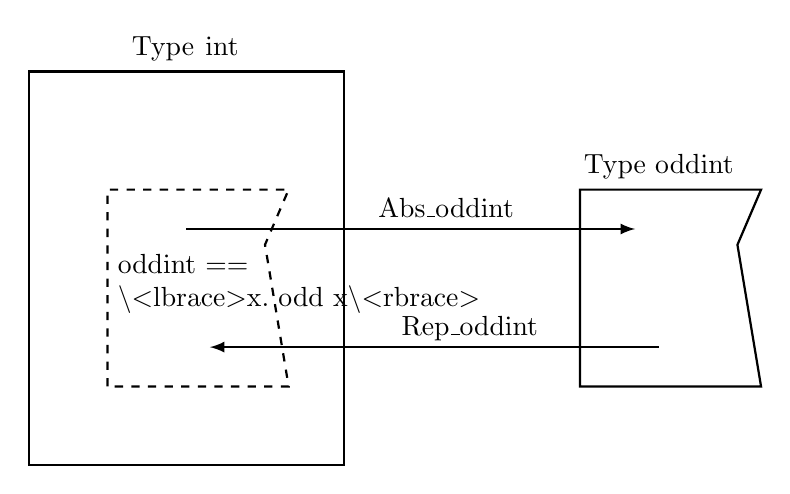
\begin{tikzpicture}
[>=latex, thick]
\draw (0,0) rectangle (4,5);
\draw [dashed] (1,1) -- (1,3.5) -- (3.3,3.5) -- (3,2.8) -- (3.3,1) -- cycle;
\draw [xshift=6cm] (1,1) -- (1,3.5) -- (3.3,3.5) -- (3,2.8) -- (3.3,1) -- cycle;
\draw (2.13,2.3) node [text width=2cm] {\isa{oddint ==}\\\isa{\<lbrace>x. odd x\<rbrace>}};
\draw [->] (2,3) -- node [anchor=base, xshift=0.45cm, yshift=0.15cm] {\isa{Abs_oddint}} (7.7,3);
\draw [->] (8.0,1.5) -- node [anchor=base, xshift=0.45cm, yshift=0.15cm] {\isa{Rep_oddint}} (2.3,1.5);
\node at (2,5) [above] {Type \isa{int}};
\node at (2,3.5) [above, xshift=6cm] {Type \isa{oddint}};
\end{tikzpicture}
\end{singlespace}

\caption{Type definition with \isa{typedef}, yielding \isa{Rep} and \isa{Abs} functions}
\label{fig:holcf-typedef}
\end{figure}

\noindent
After discharging a proof obligation that the given set \isa{\<lbrace>x::int. odd x\<rbrace>} is nonempty, the \textsc{Typedef} package generates a few constants and theorems. The set \isa{oddint} is defined equal to the set we specified; we also get a pair of \emph{representation} and \emph{abstraction} functions \isa{Rep_oddint} and \isa{Abs_oddint} that map between the set and the new type as shown in Fig.~\ref{fig:holcf-typedef}. The essential properties of these constants are listed below.

\begin{isacodes}
theorem oddint_def: "oddint == {x::int. odd x}"
theorem Rep_oddint: "Rep_oddint x \<in> oddint"
theorem Rep_oddint_inverse: "Abs_oddint (Rep_oddint x) = x"
theorem Abs_oddint_inverse: "y \<in> oddint ==> Rep_oddint (Abs_oddint y) = y"
\end{isacodes}

\noindent
We can use \isa{Rep_oddint} and \isa{Abs_oddint} to define new operations on type \isa{oddint}, like the function \isa{oddmult} below. Properties like associativity of \isa{oddmult} can then be proved using theorems provided by \textsc{Typedef}.

\begin{isacode}
definition oddmult :: "oddint => oddint => oddint"
  where "oddmult x y = Abs_oddint (Rep_oddint x * Rep_oddint y)"
\end{isacode}

All of the generated theorems about \isa{Rep_oddint} and \isa{Abs_oddint} are derived from a single axiom of the form \isa{"type_definition Rep_oddint Abs_oddint oddint"}, where the \isa{type_definition} predicate is defined as follows.\footnote{Actually, it is defined with the \isa{locale} command, not with \isa{definition}; but the distinction is not important.}

\indexdef{type_definition}
\begin{isacode}
definition type_definition :: "('b => 'a) => ('a => 'b) => 'a set => bool"
  where "type_definition Rep Abs A ==
  (\<forall>x. Rep x \<in> A) \<and> (\<forall>x. Abs (Rep x) = x) \<and> (\<forall>y. y \<in> A --> Rep (Abs y) = y)"
\end{isacode}

\noindent
The \textsc{Typedef} package includes a small library of lemmas, each with an assumption of the form \isa{"type_definition Rep Abs A"}. By instantiating these with a particular type definition axiom, \textsc{Typedef} generates all the theorems about those particular \isa{Rep} and \isa{Abs} functions.

The \textsc{Cpodef} package includes a similar library of lemmas with \isa{type_definition} assumptions. Some of these lemmas are used to derive the theorems that the package generates; others are used to discharge class instance proofs.

\paragraph{Proving a subtype is a partial order.} The first lemma in the \textsc{Cpodef} library is \isa{typedef_po}, which is used for proving \isa{po} class instances.

\indexthm{typedef_po}
\begin{isacode}
lemma typedef_po:
  fixes Rep :: "'b::below \<Rightarrow> 'a::po" and Abs :: "'a \<Rightarrow> 'b" and A :: "'a set"
  assumes type: "type_definition Rep Abs A"
  assumes below_def: "(op \<sqsubseteq>) \<equiv> (\<lambda>x y. Rep x \<sqsubseteq> Rep y)"
  shows "OFCLASS('b, po_class)"
\end{isacode}

\noindent
The conclusion of the lemma is a special predicate stating that type \isa{'b} satisfies all the axioms of class \isa{po}; it is precisely the proof obligation that users are faced with when they instantiate class \isa{po} with Isabelle's \isa{instance} command. For class \isa{po}, we must show that \isa{(op \<sqsubseteq>)} is reflexive, transitive, and antisymmetric. Reflexivity and transitivity on type \isa{'b} follow directly from the same properties on type \isa{'a}, after unfolding \isa{below_def}. Proving antisymmetry also requires injectivity of \isa{Rep}, which follows from assumption \isa{type}.

\paragraph{Proving a subtype is a cpo.} The next few lemmas in the \textsc{Cpodef} library are related to completeness and continuity. Note that these lemmas have some additional type class constraints on types \isa{'a} and \isa{'b}. Each lemma also has a new assumption \isa{adm_A} that asserts the chain-completeness of set \isa{A}. The first lemma, \isa{typedef_is_lub}, shows how to construct least upper bounds for chains on type \isa{'b}.

\indexthm{typedef_is_lub}
\begin{isacode}
lemma typedef_is_lub:
  fixes Rep :: "'b::po \<Rightarrow> 'a::cpo" and Abs :: "'a \<Rightarrow> 'b" and A :: "'a set"
  assumes type: "type_definition Rep Abs A"
  assumes below_def: "(op \<sqsubseteq>) \<equiv> (\<lambda>x y. Rep x \<sqsubseteq> Rep y)"
  assumes adm_A: "adm (\<lambda>x. x \<in> A)"
  shows "chain Y ==> range Y <<| Abs (\<Squnion>i. Rep (Y i))"
\end{isacode}

\noindent
Note that in order to show that any particular \isa{x :: 'b} is the least upper bound of a chain \isa{Y}, it suffices to show that \isa{Rep x} is the least upper bound of \isa{Rep} mapped over \isa{Y}. Accordingly, we will show \isa{range (\<lambda> i. Rep (Y i)) <<| Rep (Abs (\<Squnion>i. Rep (Y i)))}. From \isa{type}, we know that every \isa{Rep (Y i) \<in> A}; together with \isa{adm_A} we then have that \isa{(\<Squnion>i. Rep (Y i)) \<in> A}. In turn, this implies that \isa{Rep (Abs (\<Squnion>i. Rep (Y i)))} equals \isa{(\<Squnion>i. Rep (Y i))}, so our goal simplifies to \isa{range (\<lambda> i. Rep (Y i)) <<| (\<Squnion>i. Rep (Y i))}. This final goal is true because \isa{(\<lambda>i. Rep (Y i))} is a chain on a cpo type; this concludes the proof.

From lemma \isa{typedef_is_lub}, it is a simple matter to derive the lemma \isa{typedef_cpo}, which shows \isa{OFCLASS('b, cpo_class)} from the same assumptions. Another direct corollary of \isa{typedef_is_lub} is \isa{typedef_thelub}, which concludes that \isa{(\<Squnion>i. Y i)} equals \isa{Abs (\<Squnion>i. Rep (Y i))} for any chain \isa{Y}.

\paragraph{Continuity of Rep and Abs.} The next pair of lemmas show that the \isa{Rep} and \isa{Abs} functions are both continuous.

\indexthm{typedef_cont_Rep}
\begin{isacode}
lemma typedef_cont_Rep:
  fixes Rep :: "'b::cpo \<Rightarrow> 'a::cpo" and Abs :: "'a \<Rightarrow> 'b" and A :: "'a set"
  assumes type: "type_definition Rep Abs A"
  assumes below_def: "(op \<sqsubseteq>) \<equiv> (\<lambda>x y. Rep x \<sqsubseteq> Rep y)"
  assumes adm_A: "adm (\<lambda>x. x \<in> A)"
  shows "cont Rep"
\end{isacode}

\noindent
The proof of \isa{typedef_cont_Rep} starts by applying the standard rule for continuity. We must show that \isa{range (\<lambda> i. Rep (Y i)) <<| Rep (\<Squnion>i. Y i)} for an arbitrary chain \isa{Y}. After substituting lemma \isa{typedef_thelub}, our proof obligation becomes \isa{range (\<lambda> i. Rep (Y i)) <<| Rep (Abs (\<Squnion>i. Rep (Y i)))}, which we have already established while proving \isa{typedef_is_lub}.

The formulation of the continuity rule for \isa{Abs} is a little different than the rule for \isa{Rep}. Because the behavior of \isa{Abs} is unspecified on inputs not in \isa{A}, we cannot prove that \isa{Abs} is always continuous; instead we prove that \isa{Abs} is continuous when composed with another continuous function \isa{f} whose range is a subset of \isa{A}.

\indexthm{typedef_cont_Abs}
\begin{isacode}
lemma typedef_cont_Abs:
  fixes Rep :: "'b::cpo \<Rightarrow> 'a::cpo" and Abs :: "'a \<Rightarrow> 'b" and A :: "'a set"
  assumes type: "type_definition Rep Abs A"
  assumes below_def: "(op \<sqsubseteq>) \<equiv> (\<lambda>x y. Rep x \<sqsubseteq> Rep y)"
  assumes adm_A: "adm (\<lambda>x. x \<in> A)"
  shows "(\<And>x. f x \<in> A) ==> cont f ==> cont (\<lambda>x. Abs (f x))"
\end{isacode}

\noindent
The proof of \isa{typedef_cont_Abs} is by unfolding the definitions of continuity and least upper bounds, and simplifying with the rule \isa{Rep (Abs (f x)) = f x} (derived from \isa{type} and the assumption about \isa{f}.) The assumption \isa{adm_A} is actually not necessary, but the implementation of \textsc{Cpodef} is simpler when all the lemmas have the same set of assumptions.

\paragraph{Compactness.} We prove that an element \isa{x :: 'b} is compact whenever \isa{Rep x} is.

\indexthm{typedef_compact}
\begin{isacode}
lemma typedef_compact:
  fixes Rep :: "'b::cpo \<Rightarrow> 'a::cpo" and Abs :: "'a \<Rightarrow> 'b" and A :: "'a set"
  assumes type: "type_definition Rep Abs A"
  assumes below_def: "(op \<sqsubseteq>) \<equiv> (\<lambda>x y. Rep x \<sqsubseteq> Rep y)"
  assumes adm_A: "adm (\<lambda>x. x \<in> A)"
  shows "compact (Rep k) ==> compact k"
\end{isacode}
%
We assume \isa{compact (Rep k)}, which by definition means \isa{adm (\<lambda>x. Rep k \<notsqsubseteq> x)}. Then using the continuity of \isa{Rep}, lemma \isa{adm_subst} gives us \isa{adm (\<lambda>x. Rep k \<notsqsubseteq> Rep x)}. Using \isa{below_def}, we see that this is equivalent to \isa{adm (\<lambda>x. k \<notsqsubseteq> x)}, which is the definition of \isa{compact k}.

\paragraph{Proving a subtype is pointed.} The last few theorems in the \textsc{Cpodef} library are about bottoms and the \isa{pcpo} class. If the defining set \isa{A} contains \isa{\<bottom>}, then the type \isa{'b} will have a least element.

\indexthm{typedef_pcpo}
\begin{isacode}
lemma typedef_pcpo:
  fixes Rep :: "'b::cpo \<Rightarrow> 'a::pcpo" and Abs :: "'a \<Rightarrow> 'b" and A :: "'a set"
  assumes type: "type_definition Rep Abs A"
  assumes below_def: "(op \<sqsubseteq>) \<equiv> (\<lambda>x y. Rep x \<sqsubseteq> Rep y)"
  assumes bottom: "\<bottom> \<in> A"
  shows "OFCLASS('b, pcpo_class)"
\end{isacode}

\noindent
The proof is straightforward, and involves showing that \isa{Abs \<bottom>} is the minimal element of type \isa{'b}. Finally we proceed to prove lemmas \isa{Rep_strict} and \isa{Abs_strict}, which respectively conclude \isa{Rep \<bottom> = \<bottom>} and \isa{Abs \<bottom> = \<bottom>} from the same assumptions, using similar reasoning.

\paragraph{Implementing the commands.} The \isa{cpodef} and \isa{pcpodef} commands each have an input syntax identical to the \isa{typedef} command, but they differ in the proof obligations they require of the user. Figure~\ref{fig:holcf-cpodef} shows the precise proof obligations required by each tool. Additionally, each command has different class requirements on the representation type. For example, \isa{cpodef} can only be used to define sub-cpos of types that are already in class \isa{cpo}.

\begin{figure}
\centering
\begin{tabular}{|l|l|l|}
\hline
Command & Type class & Proof obligation \\
\hline\hline
\textsf{\textbf{typedef}} & \textsf{type} & \textsf{$\exists$x. x $\in$ A} \\
\hline
\textsf{\textbf{cpodef}} & \textsf{cpo} & \textsf{($\exists$x. x $\in$ A) $\land$ adm ($\lambda$x. x $\in$ A)} \\
\hline
\textsf{\textbf{pcpodef}} & \textsf{pcpo} & \textsf{$\bot$ $\in$ A $\land$ adm ($\lambda$x. x $\in$ A)} \\
\hline
\end{tabular}
\caption{Comparison of \isa{typedef}, \isa{cpodef}, and \isa{pcpodef} commands}
\label{fig:holcf-cpodef}
\end{figure}

When the \isa{cpodef} command is used, the \textsc{Cpodef} package first obtains proofs of \isa{\<exists>x. x \<in> A} and \isa{adm (\<lambda>x. x \<in> A)} from the user. The tool then uses the nonemptiness proof to call the \isa{typedef} command internally, yielding a \isa{type_definition} theorem. The tool then instantiates class \isa{below} by defining \isa{(op \<sqsubseteq>) \<equiv> (\<lambda>x y. Rep x \<sqsubseteq> Rep y)} on the new type, and uses lemma \isa{typedef_po} to prove an instance for class \isa{po}. Next, it uses the admissibility proof with lemma \isa{typedef_cpo} to prove the \isa{cpo} class instance. Finally, it instantiates lemmas like \isa{typedef_cont_Rep}, \isa{typedef_cont_Abs} and \isa{typedef_compact}, and binds them to new type-specific theorem names. More details about the generated theorems can be found in the upcoming sections.

%The \isa{pcpodef} command starts by obtaining proofs of \isa{\<bottom> \<in> A} and \isa{adm (\<lambda>x. x \<in> A)} from the user.
%The \isa{pcpodef} command starts by asking the user for proofs of \isa{\<bottom> \<in> A} and \isa{adm (\<lambda>x. x \<in> A)}.
The \isa{pcpodef} command starts by obtaining a proof of \isa{\<bottom> \<in> A \<and> adm (\<lambda>x. x \<in> A)} from the user.
From \isa{\<bottom> \<in> A}, the tool derives \isa{\<exists>x. x \<in> A}, which is used to call \isa{cpodef} internally; this yields \isa{type_definition} and \isa{below_def} theorems, and a \isa{cpo} class instance. Next it can use lemma \isa{typedef_pcpo} to prove the \isa{pcpo} class instance. Finally, it instantiates the strictness theorems for \isa{Rep} and \isa{Abs} and gives them type-specific theorem names (see Sec.~\ref{sec:holcf-sprod} for a specific example).

%%%%%%%%%%%%%%%%%%%%%%%%%%%%%%%%%%%%%%%%%%%%%%%%%%%%%%%%%%%%%%%%%%%%%%

\section{HOLCF types}
\label{sec:holcf-types}

HOLCF provides types corresponding to all of the basic constructions of domain theory, with instances of the \isa{cpo} and \isa{pcpo} classes, as appropriate. The remainder of this section is devoted to the definitions, operations, and properties of these types as formalized in \HOLCF{11}: cartesian product (\S\ref{sec:holcf-prod}), full function space (\S\ref{sec:holcf-fun}), continuous function space (\S\ref{sec:holcf-cfun}), lifted cpo (\S\ref{sec:holcf-u}), discrete cpos and flat lifted types (\S\ref{sec:holcf-lift}), strict product (\S\ref{sec:holcf-sprod}), and strict sum (\S\ref{sec:holcf-ssum}).

%%%%%%%%%%%%%%%%%%%%%%%%%%%%%%%%%%%%%%%%%%%%%%%%%%%%%%%%%%%%%%%%%%%%%%

\subsection{Cartesian product cpo}
\label{sec:holcf-prod}

If $D$ and $E$ are cpos, then the cartesian product $D \times E$ also forms a cpo, with the componentwise ordering: $(x_1, y_1) \sqsubseteq (x_2, y_2)$ if and only if $x_1 \sqsubseteq x_2 \land y_1 \sqsubseteq y_2$. Least upper bounds are also computed componentwise. If $D$ and $E$ both have bottom elements, then $D \times E$ has a minimal element $\bot = (\bot, \bot)$.

In \HOLCF{11}, as with earlier versions of HOLCF, the product cpo is formalized by providing class instances for the existing Isabelle/HOL product type \isa{'a \<times> 'b}. Isabelle type classes with overloaded constants are instantiated with the \isa{instantiation} command (for classes that fix no new constants, a simpler \isa{instance} command suffices). With the following \isa{instantiation} command block, we define the ordering on type \isa{'a \<times> 'b} (which is infix syntax for the type \isa{('a, 'b) prod}) in terms of the orderings on types \isa{'a} and \isa{'b}, which are in turn assumed to be in class \isa{below}. Because class \isa{below} asserts no axioms, the instance proof is trivial (using the ``\isa{..}'' proof method).

\indexdef{below_prod_def}
\begin{isacode}
instantiation prod :: (below, below) below
begin
  definition below_prod_def:
    "(op \<sqsubseteq>) \<equiv> (\<lambda>p1 p2. fst p1 \<sqsubseteq> fst p2 \<and> snd p1 \<sqsubseteq> snd p2)"
  instance ..
end
\end{isacode}

\noindent
Next, the following instance declarations assert that type \isa{'a \<times> 'b} is in class \isa{po} whenever both \isa{'a} and \isa{'b} are, and that a similar relationship holds for classes \isa{cpo} and \isa{pcpo}. Each \isa{instance} command yields a proof obligation, but the proofs are completely standard, so we omit them here.

\begin{isacodes}
instance prod :: (po, po) po
instance prod :: (cpo, cpo) cpo
instance prod :: (pcpo, pcpo) pcpo
\end{isacodes}

\noindent
We prove all the usual theorems about ordering, least upper bounds, continuity, and strictness for the operations of \isa{Pair}, \isa{fst}, and \isa{snd}.

\indexthm{Pair_below_iff}
\indexthm{lub_Pair}
\indexthm{cont_fst}
\indexthm{cont_snd}
\indexthm{cont2cont_Pair}
\indexthm{fst_strict}
\indexthm{snd_strict}
\indexthm{Pair_strict}
\begin{isacodes}
lemma Pair_below_iff: "(a, b) << (c, d) <-> a << c \<and> b << d"
lemma lub_Pair: "[|chain X; chain Y|] ==> (\<Squnion>i. (X i, Y i)) = (\<Squnion>i. X i, \<Squnion>i. Y i)"
lemma cont_fst: "cont fst"
lemma cont_snd: "cont snd"
lemma cont2cont_Pair: "[|cont f; cont g|] ==> cont (\<lambda>x. (f x, g x))"
lemma fst_strict: "fst \<bottom> = \<bottom>"
lemma snd_strict: "snd \<bottom> = \<bottom>"
lemma Pair_strict: "(\<bottom>, \<bottom>) = \<bottom>"
\end{isacodes}

\noindent
One lemma that is new in \HOLCF{11} is the compactness property for the \isa{Pair} constructor:

\indexthm{compact_Pair}
\begin{isacode}
lemma compact_Pair: "[|compact x; compact y|] ==> compact (x, y)"
\end{isacode}

\noindent
The proof starts by applying the standard introduction rule for compactness, so we have the goal \isa{adm (\<lambda>z. (x, y) \<notsqsubseteq> z)}. Simplifying with the definition of ordering on the product type, this becomes \isa{adm (\<lambda>z. x \<notsqsubseteq> fst z \<or> y \<notsqsubseteq> snd z)}. Finally, this is solved using lemmas \isa{adm_disj}, \isa{adm_compact_not_below}, \isa{cont_fst}, and \isa{cont_snd}, with the assumptions about \isa{x} and \isa{y}.

%%%%%%%%%%%%%%%%%%%%%%%%%%%%%%%%%%%%%%%%%%%%%%%%%%%%%%%%%%%%%%%%%%%%%%

\subsection{Full function space cpo}
\label{sec:holcf-fun}

If $D$ is an arbitrary set, and $E$ is a cpo, then the full function space $D \Rightarrow E$ forms a cpo when the functions are given the pointwise ordering. If $E$ has a bottom element, then $D \Rightarrow E$ contains a minimal element.

\HOLCF{11} provides the following class instances for the full function space type \isa{'a => 'b}. As with the product type, the proofs are the same standard ones used in previous HOLCF versions, so we just summarize the basic results.

\begin{isacodes}
instance "fun" :: (type, po) po
instance "fun" :: (type, cpo) cpo
instance "fun" :: (type, pcpo) pcpo
\end{isacodes}

\noindent
We prove the usual lemmas about ordering, least upper bounds, strictness and continuity:

\indexthm{fun_below_iff}
\indexthm{thelub_fun}
\indexthm{app_strict}
\indexthm{cont2cont_fun}
\indexthm{cont2cont_lambda}
\begin{isacodes}
lemma fun_below_iff: "(f << g) = (\<forall>x. f x << g x)"
lemma thelub_fun: "chain (Y::nat => 'a => 'b) ==> (\<Squnion>i. Y i) = (\<lambda>x. \<Squnion>i. Y i x)"
lemma app_strict: "\<bottom> x = \<bottom>"
lemma cont2cont_fun: "cont f ==> cont (\<lambda>x. f x y)"
lemma cont2cont_lambda: "[|!!y. cont (\<lambda>x. f x y)|] ==> cont (\<lambda>x y. f x y)"
\end{isacodes}

%%%%%%%%%%%%%%%%%%%%%%%%%%%%%%%%%%%%%%%%%%%%%%%%%%%%%%%%%%%%%%%%%%%%%%

\subsection{Continuous function type}
\label{sec:holcf-cfun}

In domain theory, the continuous function space $[D \to E]$ consists of the set of all continuous functions between cpos $D$ and $E$. Ordered pointwise, $[D \to E]$ forms a cpo, and it has a least element whenever $E$ does. In \HOLCF{11}, we define the continuous function type \isa{'a -> 'b} to be isomorphic to a subset of the full function type \isa{'a => 'b}, using the \isa{cpodef} command.

\begin{isacode}
cpodef ('a, 'b) cfun (infixr "->" 0) = "{f::('a::cpo => 'b::cpo). cont f}"
\end{isacode}

\noindent
Two proof obligations are required for this definition to be accepted: For nonemptiness, we must show that there exists a continuous function of type \isa{'a => 'b} (any constant function will do). For admissibility, we must show that the lub of a chain of continuous functions is continuous, which is an easy corollary of lemma \isa{cont2cont_lub} (Sec.~\ref{sec:holcf-cont}). Once the type definition is processed we get the following representation and abstraction functions.

\begin{isacodes}
Rep_cfun :: ('a -> 'b) => ('a => 'b)
Abs_cfun :: ('a => 'b) => ('a -> 'b)
\end{isacodes}

\noindent
The HOLCF notations for continuous application and abstraction are really just abbreviations for these constants: The syntax \isa{f`x} represents \isa{Rep_cfun f x}, and \isa{(\<Lambda> x. t)} represents \isa{Abs_cfun (\<lambda>x. t)}.

The \isa{cpodef} command also generates several theorems, including those listed in Fig.~\ref{fig:holcf-cfun-cpodef}. Some of these are produced by the \textsc{Typedef} package, but the last few are added by \textsc{Cpodef}.

\begin{figure}
\indexdef{cfun}
\indexthm{Rep_cfun_inverse}
\indexthm{Abs_cfun_inverse}
\indexthm{Rep_cfun}
\indexthm{Rep_cfun_inject}
\indexthm{below_cfun_def}
\indexthm{cont_Rep_cfun}
\indexthm{cont_Abs_cfun}
\begin{isabelle}
definition cfun_def: "cfun \<equiv> {f. cont f}"
theorem Rep_cfun_inverse: "Abs_cfun (Rep_cfun x) = x"
theorem Abs_cfun_inverse: "y \<in> cfun ==> Rep_cfun (Abs_cfun y) = y"
theorem Rep_cfun: "Rep_cfun x \<in> cfun"
theorem Rep_cfun_inject: "(Rep_cfun x = Rep_cfun y) = (x = y)"
definition below_cfun_def: "(op \<sqsubseteq>) \<equiv> (\<lambda>x y. Rep_cfun x \<sqsubseteq> Rep_cfun y)"
theorem cont_Rep_cfun: "cont f ==> cont (\<lambda>x. Rep_cfun (f x))"
theorem cont_Abs_cfun: "[|!!x. f x \<in> cfun; cont f|] ==> cont (\<lambda>x. Abs_cfun (f x))"
\end{isabelle}
\caption{Selected theorems generated by \isa{cpodef} for continuous function type}
\label{fig:holcf-cfun-cpodef}
\end{figure}

Several of the key properties about the continuous function space are derived fairly directly from the theorems produced by \textsc{Cpodef}; Fig.~\ref{fig:holcf-cfun-rules} lists these. Extensionality follows from \isa{Rep_cfun_inject}; extensionality of function inequality is a consequence of \isa{below_cfun_def}. We get eta-conversion from \isa{Rep_cfun_inverse}, while beta-conversion (with a continuity side-condition) follows from \isa{Abs_cfun_inverse}. The continuous application operator \isa{Rep_cfun} can be proved continuous in its first argument using \isa{cont_Rep_cfun}, and in its second using \isa{Rep_cfun}; these lemmas can then be combined into a single continuity rule using lemma \isa{cont_apply}. Finally, a continuity rule for continuous abstraction follows from rule \isa{cont_Abs_cfun}.

\begin{figure}
\indexthm{cfun_eq_iff}
\indexthm{cfun_below_iff}
\indexthm{eta_cfun}
\indexthm{beta_cfun}
\indexthm{cont_Rep_cfun1}
\indexthm{cont_Rep_cfun2}
\indexthm{cont2cont_APP}
\indexthm{cont2cont_LAM}
\begin{isabelle}
lemma cfun_eq_iff: "(f = g) = (\<forall>x. f`x = g`x)"
lemma cfun_below_iff: "(f << g) = (\<forall>x. f`x << g`x)"
lemma eta_cfun: "(\<Lambda> x. f`x) = f"
lemma beta_cfun: "cont f ==> (\<Lambda> x. f x)`u = f u"
lemma cont_Rep_cfun1: "cont (%f. f`x)"
lemma cont_Rep_cfun2: "cont (%x. f`x)"
lemma cont2cont_APP: "[|cont (%x. f x); cont (%x. t x)|] ==> cont (%x. (f x)`(t x))"
\end{isabelle}
\vspace{-2.5\medskipamount}
\begin{isacode}
lemma cont2cont_LAM:
  "[|!!x. cont (%y. f x y); !!y. cont (%x. f x y)|] ==> cont (%x. \<Lambda> y. f x y)"
\end{isacode}
\caption{Properties of continuous functions, derived from \isa{cpodef} theorems}
\label{fig:holcf-cfun-rules}
\end{figure}

The \isa{cpodef} command automatically proves that type \isa{'a -> 'b} is an instance of class \isa{cpo} (as long as \isa{'a} and \isa{'b} are also cpos, as required by the definition). But we should also like to reason about the bottom element of type \isa{'a -> 'b}, which must exist whenever type \isa{'b} is pointed. Therefore we prove the following class instance.
%
\begin{isacode}
instance cfun :: (cpo, pcpo) pcpo
\end{isacode}
%
We prove the instance using \isa{typedef_pcpo}, the same lemma used internally by the \isa{pcpodef} command. As a proof obligation, we must show that \isa{(\<bottom>::'a => 'b) \<in> cfun}. From the theory of the full function space, we know that \isa{\<bottom> = (\<lambda>x. \<bottom>)}, which is continuous because it is a constant function. Using lemmas \isa{typedef_Rep_strict} and \isa{typedef_Abs_strict}, we can then show that \isa{Rep_cfun} and \isa{Abs_cfun} are strict:
%
\indexthm{APP_strict}
\indexthm{LAM_strict}
\begin{isacodes}
lemma APP_strict: "\<bottom>`x = \<bottom>"
lemma LAM_strict: "(\<Lambda> x. \<bottom>) = \<bottom>"
\end{isacodes}
%
\HOLCF{11} also defines a few useful operations for the continuous function type. The identity and composition operator are straightforward and require little discussion; they have been present in all versions of HOLCF. The abstractions used in their definitions are easily shown to be continuous, so there is no obstacle to unfolding and beta-reducing their definitions. The theory defines infix syntax \isa{f oo g} to represent \isa{cfcomp`f`g}.
%
\indexdef{ID}
\begin{isacode}
definition ID :: "'a -> 'a"
  where "ID = (\<Lambda> x. x)"
\end{isacode}
\unmedskip
\indexdef{cfcomp}
\begin{isacode}
definition cfcomp :: "('b -> 'c) -> ('a -> 'b) -> 'a -> 'c"
  where "cfcomp = (\<Lambda> f g x. f`(g`x))"
\end{isacode}
%
The next operation in the continuous function theory is \isa{seq}, which can be used to construct strict functions; it is new for \HOLCF{11}. It takes two arguments \isa{x} and \isa{y}; the result is \isa{\<bottom>} when \isa{x = \<bottom>} and \isa{y} otherwise.\footnote{Haskell programmers may recognize this as the Haskell primitive \hs{seq}, which has the same semantics.} In the upcoming sections, we will see that it is useful for defining several operations on the strict product and strict sum types.
%
\indexdef{seq}
\begin{isacode}
definition seq :: "'a::pcpo -> 'b::pcpo -> 'b"
  where "seq = (\<Lambda> x. if x = \<bottom> then \<bottom> else ID)"
\end{isacode}
%
Proving that the body of \isa{seq} is continuous is a bit more difficult than for \isa{ID} or \isa{cfcomp}. To prove continuity, we must show for an arbitrary chain \isa{Y} that \isa{(if (\<Squnion>i. Y i) = \<bottom> then \<bottom> else ID)} is a least upper bound of the sequence given by \isa{(\<lambda>i. if Y i = \<bottom> then \<bottom> else ID)}. The proof proceeds using a lemma about least upper bounds:
%
\indexthm{lub_eq_bottom_iff}
\begin{isacode}
lemma lub_eq_bottom_iff: "chain Y ==> (\<Squnion>i. Y i) = \<bottom> <-> (\<forall>i. Y i = \<bottom>)"
\end{isacode}
%
By unfolding the definition of least upper bound, and using \isa{lub_eq_bottom_iff} as a rewrite rule, we can prove continuity of \isa{seq} using Isabelle's simplifier. The simplifier automatically performs the necessary case splits on if-then-else expressions. We prove the following rules about \isa{seq}, and add some of them to the simplifier:
%
\indexthm{seq_conv_if}
\begin{isacode}
lemma seq_conv_if: "seq`x = (if x = \<bottom> then \<bottom> else ID)"
\end{isacode}
\unmedskip
\indexthm{seq_simps}
\begin{isacode}
lemma seq_simps [simp]:
  "seq`\<bottom> = \<bottom>"
  "seq`x`\<bottom> = \<bottom>"
  "x ~= \<bottom> ==> seq`x = ID"
\end{isacode}
%
The older HOLCF function \isa{strictify}, which takes a function argument and returns a strict function, is now defined in terms of \isa{seq} as follows.
%
\indexdef{strictify}
\begin{isacode}
definition strictify :: "('a::pcpo -> 'b::pcpo) -> 'a -> 'b"
  where "strictify = (\<Lambda> f x. seq`x`(f`x))"
\end{isacode}
\unmedskip

%%%%%%%%%%%%%%%%%%%%%%%%%%%%%%%%%%%%%%%%%%%%%%%%%%%%%%%%%%%%%%%%%%%%%%

\subsection{Lifted cpo}
\label{sec:holcf-u}

Lifting is a way to create a new pointed cpo from any given cpo, by adding a new bottom element (see Fig.~\ref{fig:holcf-lifted-cpo}). If $D$ is a cpo (which may or may not have a least element), then the lifted cpo $D_\bot$ consists of $\bot$ and values of the form $\mathit{up}(x)$ where $x\in D$. Furthermore, the constructor $\mathit{up} : D \to D_\bot$ is non-strict, that is, $\mathit{up}(x) \neq \bot$ for any $x \in D$. In particular, if $D$ has a bottom element we have $\mathit{up}(\bot) \neq \bot$.

\begin{figure}
\centering
\begin{tikzpicture}
  \draw (0,0.5) -- (2,3) -- (-2,3) -- cycle;
  \draw (0,0) -- (0,0.5);
  \fill (0,0) circle (0.06);
\end{tikzpicture}
\caption{Lifted cpo}
\label{fig:holcf-lifted-cpo}
\end{figure}
 
In HOLCF, the lifted cpo is formalized by the type constructor \isa{'a u}, which is defined using the Isabelle/HOL \textsc{Datatype} package.\footnote{The name \isa{'a u} was inherited from earlier LCF provers. Perhaps \isa{'a lift} would be a more apt name, but it is already taken in HOLCF (see \S\ref{sec:holcf-lift}).} (We also define \isa{'a\<lifted>} as an alternative syntax to \isa{'a u}.)
%
\begin{isacode}
datatype 'a u = Ibottom | Iup 'a
\end{isacode}
%
Next we instantiate class \isa{below} for type \isa{'a\<lifted>} (requiring \isa{'a} to be in class \isa{cpo}). We define the ordering in the expected way, with \isa{Ibottom} as the least element.
%
\indexthm{below_up_def}
\begin{isacode}
instantiation u :: (cpo) below
begin
  definition below_up_def: "(x \<sqsubseteq> y) =
    (case x of Ibottom => True | Iup a =>
      (case y of Ibottom => False | Iup b => a \<sqsubseteq> b))"
  instance ..
end
\end{isacode}
%
It is straightforward to show that type \isa{'a\<lifted>} is a partial order: The proofs of reflexivity, transitivity, and antisymmetry proceed by case analysis. Proving the \isa{cpo} instance requires more work. In order to show chain-completeness of the lifted cpo type, we prove a case analysis lemma for chains of type \isa{nat => 'a\<lifted>}.
%
\indexthm{up_chain_lemma}
\begin{isacode}
lemma up_chain_lemma:
  assumes "chain Y"
  shows "(\<forall>i. Y i = Ibottom) \<or>
    (\<exists>A k. (\<forall>i. Iup (A i) = Y (i + k)) \<and> chain A \<and> range Y <<| Iup (\<Squnion>i. A i))"
\end{isacode}
%
In the first case, a chain \isa{Y} might be constantly \isa{Ibottom}: In this case the least upper bound of \isa{Y} is \isa{Ibottom}. Otherwise, \isa{Y} has an initial segment of zero or more \isa{Ibottom} terms, followed by the \isa{Iup} constructor mapped over a chain \isa{A :: nat => 'a}. In this case, \isa{Iup (\<Squnion> i. A i)} gives the least upper bound of chain \isa{Y}; showing this requires a lemma stating that shifting a sequence preserves the least upper bound. Thus, by case analysis on chains, we prove that \isa{'a\<lifted>} is a cpo. Proving the \isa{pcpo} class instance is easy, because \isa{Ibottom} is the minimal element of the type.

With the class instances finished, we can now define operations on type \isa{'a\<lifted>} with continuous function types. We start with the constructor \isa{up}.
%
\indexdef{up}
\begin{isacode}
definition up :: "'a -> 'a\<lifted>" where "up = (\<Lambda> a. Iup a)"
\end{isacode}
%
It is relatively simple to prove that \isa{Iup} preserves least upper bounds (and is therefore continuous), by unfolding the definitions and calling the simplifier. Now knowing \isa{Ibottom = \<bottom>} and \isa{Iup x = up`x}, we can prove new versions of the case-analysis and induction rules for type \isa{'a\<lifted>} in terms of \isa{\<bottom>} and \isa{up} instead of \isa{Ibottom} and \isa{Iup}. We similarly derive the ordering properties and injectivity of \isa{up} from the same properties of \isa{Iup}.
%
\indexthm{up_defined}
\indexthm{up_eq}
\indexthm{up_below}
\begin{isacodes}
lemma up_defined [simp]: "up`x ~= \<bottom>"
lemma up_eq [simp]: "(up`x = up`y) = (x = y)"
lemma up_below [simp]: "(up`x \<sqsubseteq> up`y) = (x \<sqsubseteq> y)"
\end{isacodes}
%
To prove that the \isa{up} constructor preserves compactness requires unfolding the definitions and reasoning by cases on chains, using \isa{up_chain_lemma}.
\indexthm{compact_up}
\begin{isacode}
lemma compact_up: "compact x ==> compact (up`x)"
\end{isacode}

\noindent
Next, we define the case combinator for type \isa{'a\<lifted>}, called \isa{fup}.
\indexdef{fup}
\begin{isacode}
definition fup :: "('a -> 'b::pcpo) -> 'a\<lifted> -> 'b"
  where "fup = (\<Lambda> f x. case x of Ibottom => \<bottom> | Iup a => f`a)"
\end{isacode}
It is easy to prove that the body of \isa{fup} is continuous in \isa{f}, by case analysis on \isa{x}. To show that the body of \isa{fup} is continuous in \isa{x} requires using \isa{up_chain_lemma} again, along with more reasoning about least upper bounds of shifted chains. The case combinator obeys the following rules:
\indexthm{fup_simps}
\begin{isacode}
lemma fup_simps [simp]:
  "fup`f`\<bottom> = \<bottom>"
  "fup`f`(up`x) = f`x"
\end{isacode}
We also define special syntax for \isa{fup}. The case expression \isa{(case x of up`a => t)} represents the term \isa{fup`(\<Lambda> a. t)`x}, and \isa{(\<Lambda>(up`a). t)} represents \isa{fup`(\<Lambda> a. t)}.

%%%%%%%%%%%%%%%%%%%%%%%%%%%%%%%%%%%%%%%%%%%%%%%%%%%%%%%%%%%%%%%%%%%%%%

\subsection{Cpos from HOL types}
\label{sec:holcf-lift}

In this section we will introduce two type constructors that facilitate the integration of types and terms from Isabelle/HOL with HOLCF \cite{hol+lcf}. The first, \isa{'a discr} (introduced in \HOLCF{99}), yields an unpointed discrete cpo. The second, \isa{'a lift} (present since \HOLCF{95}), adds a bottom element to yield a flat pointed cpo. The \isa{'a lift} type constructor is also used to model two of the base types from LCF: the lifted unit type \isa{one}, and the domain of truth values \isa{tr} (see Fig.~\ref{fig:holcf-flat-types}).

\begin{figure}
\centering
\subfloat[\isa{one = unit lift}]{
  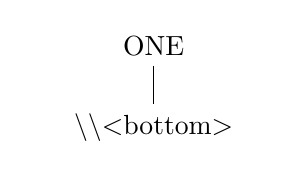
\begin{tikzpicture}
  [anchor=base]
  \node (bottom) at (0,0) {\isa{\\<bottom>}};
  \node (ONE) at (0,1) {\isa{ONE}};
  \draw (bottom) -- (ONE);
  \useasboundingbox (-1.6,0) -- (1.6,0);
  \end{tikzpicture}
}
\subfloat[\isa{tr = bool lift}]{
  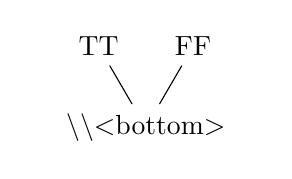
\begin{tikzpicture}
  [anchor=base]
  \node (bottom) at (0,0) {\isa{\\<bottom>}};
  \node (TT) at (-0.6,1) {\isa{TT}};
  \node (FF) at (0.6,1) {\isa{FF}};
  \draw (bottom) -- (TT);
  \draw (bottom) -- (FF);
  \useasboundingbox (-1.5,0) -- (1.5,0);
  \end{tikzpicture}
}
\subfloat[\isa{nat lift}]{
  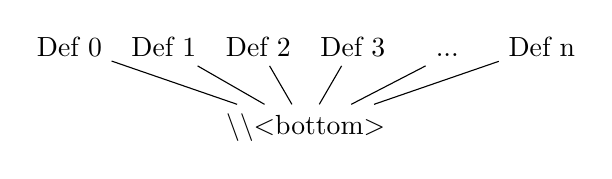
\begin{tikzpicture}
  [anchor=base]
  \node (bottom) at (0,0) {\isa{\\<bottom>}};
  \node (0) at (-3.0,1) {\isa{Def 0}};
  \node (1) at (-1.8,1) {\isa{Def 1}};
  \node (2) at (-0.6,1) {\isa{Def 2}};
  \node (3) at (0.6,1) {\isa{Def 3}};
  \node (dots) at (1.8,1) {\isa{...}};
  \node (n) at (3.0,1) {\isa{Def n}};
  \draw (bottom) -- (0);
  \draw (bottom) -- (1);
  \draw (bottom) -- (2);
  \draw (bottom) -- (3);
  \draw (bottom) -- (dots);
  \draw (bottom) -- (n);
  \end{tikzpicture}
}
\caption{Flat lifted types in HOLCF}
\label{fig:holcf-flat-types}
\end{figure}

\paragraph{Discrete cpo.} Any ordinary HOL type can be turned into a cpo by giving it a discrete ordering. In HOLCF this construction is formalized using the type \isa{'a discr}.

\indexdef{Discr}
\begin{isacode}
datatype 'a discr = Discr "'a"
\end{isacode}

\noindent
To go along with the constructor function \isa{Discr}, we define its inverse, \isa{undiscr}.

\indexdef{undiscr}
\begin{isacode}
definition undiscr :: "'a discr => 'a"
  where "undiscr x = (case x of Discr y => y)"
\end{isacode}
 
The ordering on type \isa{'a discr} is defined so that \isa{(x << y) = (x = y)}, which makes \isa{'a discr} an instance of the \isa{discrete_cpo} class (and thus also the \isa{chfin} class). In particular, this means that every function \isa{f :: 'a discr => 'b} is continuous, and every predicate \isa{P :: 'a discr => bool} is admissible.

It might make sense to define discrete orderings for various HOL types, such as \isa{bool}, \isa{nat}, and \isa{int}, making all those types instances of the \isa{discrete_cpo} class. However, this is not really necessary, because the types \isa{bool discr}, \isa{nat discr}, and \isa{int discr} can be used instead.

\HOLCF{11} does define a discrete ordering for the single-element HOL \isa{unit} type. Type \isa{unit} is special, because it is the only discrete cpo that also has a bottom element. For technical reasons, it is much simpler to make \isa{unit} an instance of class \isa{pcpo} directly than it would be to make \isa{unit discr :: pcpo}. The Isabelle type \isa{unit} corresponds to the \isa{void} type from Cambridge LCF \cite{paulson87lcf}.

\paragraph{Flat lifted type.} Any ordinary HOL type can be made into a pointed cpo by adjoining a new bottom element, and giving the new type a flat ordering (in the sense of the \isa{flat} type class described in Sec.~\ref{sec:holcf-classes}). This construction is formalized in HOLCF by the type \isa{'a lift}.

\begin{isacode}
pcpodef (open) 'a lift = "UNIV :: ('a discr)\<lifted> set"
\end{isacode}

\noindent
We use the \textsc{Cpodef} package to define \isa{'a lift} as an isomorphic copy of \isa{('a discr)\<lifted>}.\footnote{The \isa{(open)} option suppresses the definition of the set constant \isa{lift == UNIV}.}$^,$\footnote{Another sensible design choice would be to use \isa{type_synonym 'a lift = "'a discr u"}.} As such, the \isa{Rep_lift} and \isa{Abs_lift} functions form a continuous isomorphism. Next we define the constructor function, \isa{Def}.

\indexdef{Def}
\begin{isacode}
definition Def :: "'a => 'a lift"
  where "Def x = Abs_lift (up`(Discr x))"
\end{isacode}
%
Using this definition, we prove that \isa{Def} is injective and never returns \isa{\<bottom>}. It is also simple to prove an induction rule for type \isa{'a lift}, by case analysis on the representing type.

\indexthm{lift_induct}
\begin{isacode}
lemma lift_induct: "[|P \<bottom>; !!x. P (Def x)|] ==> P y"
\end{isacode}

\noindent
Using these lemmas, we then use the \isa{rep_datatype} command provided by the \textsc{Datatype} package to generate a case combinator \isa{lift_case} and various related theorems; thus we are allowed to treat \isa{Def} and \isa{\<bottom>} as constructors of an ordinary datatype.

By case analysis, and using the ordering properties of \isa{Def}, we can show that \isa{'a lift} is an instance of class \isa{flat}. Because \isa{flat} is a subclass of \isa{chfin}, this means also that every value of type \isa{'a lift} is compact.

In order to use \isa{lift_case} to define continuous functions, we need to prove a continuity rule for it. We start with a lemma that lets us express \isa{lift_case} using \isa{Rep_lift} and \isa{fup}. Having expressed \isa{lift_case} in terms of other continuous functions, it is now easy to show the continuity of \isa{lift_case}.

\indexthm{lift_case_eq}
\begin{isacode}
lemma lift_case_eq:
  "(case x of \<bottom> => \<bottom> | Def a => f a) = (case Rep_lift x of up`y => f (undiscr y))"
\end{isacode}
\unmedskip
\indexthm{cont2cont_lift_case}
\begin{isacode}
lemma cont2cont_lift_case [simp]:
  "[|!!a. cont (\<lambda>x. f x a); cont (\<lambda>x. g x)|]
    ==> cont (\<lambda>x. case g x of \<bottom> => \<bottom> | Def a => f x a)"
\end{isacode}

\noindent
To facilitate the definition of continuous functions on type \isa{'a lift}, we define combinators \isa{flift1} and \isa{flift2}. From \isa{cont2cont_lift_case}, we derive a continuity rule for \isa{flift1} (not shown).
\indexdef{flift1}
\begin{isacode}
definition flift1 :: "('a => 'b::pcpo) => ('a lift -> 'b)"
  where "flift1 f = (\<Lambda> x. case x of \<bottom> => \<bottom> | Def a => f a)"
\end{isacode}
\unmedskip
\indexdef{flift2}
\begin{isacode}
definition flift2 :: "('a => 'b) => ('a lift -> 'b lift)"
  where "flift2 f = flift1 (\<lambda>x. Def (f x))"
\end{isacode}
We also define the syntax \isa{(\<Lambda>(Def x). t)} to represent \isa{flift1 (\<lambda>x. t)}.

\paragraph{Lifted unit type.} We define the standard LCF type \isa{one} as a type synonym for \isa{unit lift}. We proceed to define the constructor \isa{ONE} and a case combinator \isa{one_case} (strict in its second argument), as shown. We also prove the expected ordering properties and rewrite rules for these constants.

\indexdef{type_synonym one}
\begin{isacode}
type_synonym one = "unit lift"
\end{isacode}
\unmedskip
\indexdef{ONE}
\begin{isacode}
definition ONE :: "one"
  where "ONE = Def ()"
\end{isacode}
\unmedskip
\indexdef{one_case}
\begin{isacode}
definition one_case :: "'a -> one -> 'a"
  where "one_case = (\<Lambda> x (Def u). x)"
\end{isacode}

\noindent
We define the syntax \isa{(case x of ONE => t)} to represent \isa{one_case`t`x}, and \isa{(\<Lambda> ONE. t)} to represent \isa{one_case`t}.

\paragraph{Lifted boolean type.} The LCF type of truth values, \isa{tr}, is defined as a synonym for \isa{bool lift}. This type has constructors \isa{TT} and \isa{FF}; its case combinator \isa{tr_case} is the continuous if-then-else operator.

\indexdef{type_synonym tr}
\begin{isacode}
type_synonym tr = "bool lift"
\end{isacode}
\unmedskip
\indexdef{TT}
\begin{isacode}
definition TT :: "tr"
  where "TT = Def True"
\end{isacode}
\unmedskip
\indexdef{FF}
\begin{isacode}
definition FF :: "tr"
  where "FF = Def False"
\end{isacode}
\unmedskip
\indexdef{tr_case}
\begin{isacode}
definition tr_case :: "'a -> 'a -> tr -> 'a"
  where "tr_case = (\<Lambda> x y (Def b). if b then x else y)"
\end{isacode}

\noindent
We define the syntax \isa{(If t then x else y)} to represent \isa{tr_case`x`y`t}. Note that we use ``\isa{If}'' with a capital letter to distinguish from the standard if-then-else operation on type \isa{bool}, which uses lowercase ``\isa{if}''.

%%%%%%%%%%%%%%%%%%%%%%%%%%%%%%%%%%%%%%%%%%%%%%%%%%%%%%%%%%%%%%%%%%%%%%

\subsection{Strict product type}
\label{sec:holcf-sprod}

The strict product (also known as ``smash product'') is one of the standard constructions in domain theory \cite{gunter90semantic, gunter92semantics, amadio+curien}. If $D$ and $E$ are pointed cpos, then $D \otimes E$ is also a pointed cpo. Its elements are strict pairs of the form $\llparenthesis x, y \rrparenthesis$, where $x \in D$ and $y \in E$. Strict pairs where either component equals $\bot$ are identified with the bottom element of $D \otimes E$, so that $\llparenthesis x, \bot \rrparenthesis = \llparenthesis \bot, y \rrparenthesis = \bot$.

In \HOLCF{11}, we define the strict product of \isa{'a} and \isa{'b} as a subset of the cartesian product type \isa{'a \<times> 'b}. The type consists of those pairs where neither element is \isa{\<bottom>}, plus the pair \isa{\<bottom> = (\<bottom>, \<bottom>)}.

\begin{isacode}
pcpodef ('a, 'b) sprod  (infixr "**" 20) =
  "{p::('a::pcpo \<times> 'b::pcpo). p = UU \<or> (fst p \<noteq> UU \<and> snd p \<noteq> UU)}"
\end{isacode}

\noindent
The proof obligations for \isa{pcpodef} are that the set contains \isa{UU}, and set membership is admissible. Both goals are solved immediately by simplification. (Note that as \isa{\<bottom>} is compact, being non-\isa{UU} is an admissible predicate.) The \textsc{Cpodef} package generates a set of lemmas analogous to those listed in Fig.~\ref{fig:holcf-cfun-cpodef}, plus a few more about the strictness of \isa{Rep_sprod} and \isa{Abs_sprod} (see Fig.~\ref{fig:holcf-sprod-pcpodef}).

\begin{figure}
\indexdef{sprod}
\indexthm{Rep_sprod_inverse}
\indexthm{Abs_sprod_inverse}
\indexthm{Rep_sprod}
\indexthm{Rep_sprod_inject}
\indexthm{below_sprod_def}
\indexthm{cont_Rep_sprod}
\indexthm{cont_Abs_sprod}
\indexthm{compact_sprod}
\indexthm{Rep_sprod_strict}
\indexthm{Abs_sprod_strict}
\begin{isabelle}
definition sprod_def: "sprod \<equiv> {p. p = UU \<or> (fst p ~= UU \<and> snd p ~= UU)}"
theorem Rep_sprod_inverse: "Abs_sprod (Rep_sprod x) = x"
theorem Abs_sprod_inverse: "y \<in> sprod ==> Rep_sprod (Abs_sprod y) = y"
theorem Rep_sprod: "Rep_sprod x \<in> sprod"
theorem Rep_sprod_inject: "(Rep_sprod x = Rep_sprod y) = (x = y)"
definition below_sprod_def: "(op \<sqsubseteq>) \<equiv> (\<lambda>x y. Rep_sprod x \<sqsubseteq> Rep_sprod y)"
theorem cont_Rep_sprod: "cont f ==> cont (\<lambda>x. Rep_sprod (f x))"
theorem cont_Abs_sprod: "[|!!x. f x \<in> sprod; cont f|] ==> cont (\<lambda>x. Abs_sprod (f x))"
theorem compact_sprod: "compact (Rep_sprod x) ==> compact x"
theorem Rep_sprod_strict: "Rep_sprod \<bottom> = \<bottom>"
theorem Abs_sprod_strict: "Abs_sprod \<bottom> = \<bottom>"
\end{isabelle}
\caption{Selected theorems generated by \isa{pcpodef} for strict product type}
\label{fig:holcf-sprod-pcpodef}
\end{figure}

\paragraph{Constructor function.} The first operation we define is the strict pair constructor, \isa{spair}. The definition uses the operator \isa{seq} to ensure that if either \isa{a} or \isa{b} is \isa{\<bottom>}, then both components of the resulting pair will be \isa{\<bottom>}.

\indexdef{spair}
\begin{isacode}
definition spair :: "'a -> 'b -> ('a ** 'b)"
  where "spair = (\<Lambda> a b. Abs_sprod (seq`b`a, seq`a`b))"
\end{isacode}

\noindent
We also define syntax for strict tuples. The expression \isa{(:a, b:)} is syntax for \isa{spair`a`b}; larger tuples nest to the right, so \isa{(:a, b, c:)} means \isa{spair`a`(spair`b`c)}.
 
In order to prove properties about \isa{spair}, we need to know how \isa{Rep_sprod} acts on it. We start by proving \isa{(seq`b`a, seq`a`b) \<in> sprod} as a lemma. Then we can use \isa{cont_Abs_sprod} and \isa{Abs_sprod_inverse} (provided by the \textsc{Cpodef} package) to beta-reduce the definition of \isa{spair} and prove the desired rule:

\indexthm{Rep_sprod_spair}
\begin{isacode}
lemma Rep_sprod_spair: "Rep_sprod (:a, b:) = (seq`b`a, seq`a`b)"
\end{isacode}

\noindent
Together with a group of other rewrite rules, the lemma \isa{Rep_sprod_spair} forms part of a general strategy for proving properties about strict products. The rules in \isa{Rep_sprod_simps} replace comparisons on type \isa{'a ** 'b} with comparisons on the component types \isa{'a} and \isa{'b}.

\indexthm{Rep_sprod_simps}
\begin{isacode}
lemma Rep_sprod_simps:
  "x = y <-> Rep_sprod x = Rep_sprod y"
  "x << y <-> Rep_sprod x << Rep_sprod y"
  "t = u <-> fst t = fst u & snd t = snd u"
  "t << u <-> fst t << fst u & snd t << snd u"
  "Rep_sprod (:a, b:) = (seq`b`a, seq`a`b)"
  "Rep_sprod UU = UU"
\end{isacode}

\noindent
Each of the following five lemmas is proved automatically by simplifying with \isa{Rep_sprod_simps}. (The if-and-only-if rules also require \isa{seq_conv_if}, so that the simplifier will do the appropriate case splits on whether or not values equal \isa{UU}.)

\indexthm{spair_strict1}
\begin{isacode}
lemma spair_strict1 [simp]: "(:\<bottom>, b:) = \<bottom>"
\end{isacode}
\unmedskip
\indexthm{spair_strict2}
\begin{isacode}
lemma spair_strict2 [simp]: "(:a, \<bottom>:) = \<bottom>"
\end{isacode}
\unmedskip
\indexthm{spair_bottom_iff}
\begin{isacode}
lemma spair_bottom_iff [simp]: "(:a, b:) = \<bottom> <-> a = \<bottom> \<or> b = \<bottom>"
\end{isacode}
\unmedskip
\indexthm{spair_below_iff}
\begin{isacode}
lemma spair_below_iff: "(:a, b:) << (:c, d:) <->
  a = \<bottom> \<or> b = \<bottom> \<or> (a << c \<and> b << d)"
\end{isacode}
\unmedskip
\indexthm{spair_eq_iff}
\begin{isacode}
lemma spair_eq_iff: "(:a, b:) = (:c, d:) <->
  (a = c \<and> b = d) \<or> ((a = \<bottom> \<or> b = \<bottom>) \<and> (c = \<bottom> \<or> d = \<bottom>))"
\end{isacode}

The same set of rewrite rules also works for proving a case analysis rule for type \isa{'a ** 'b}. The proof of \isa{sprodE} starts by inserting the fact \isa{Rep_sprod y \<in> sprod} into the goal state. Then we unfold the definition of \isa{sprod}, and use the \isa{auto} tactic to split the disjunctions and simplify.
%
\indexthm{sprodE}
\begin{isacode}
lemma sprodE:
  "[|y = UU ==> P; !!a b. [|y = (:a, b:); a ~= UU; b ~= UU|] ==> P|] ==> P"
\end{isacode}
%
The induction rule for strict products is a direct consequence of the case analysis rule.
%
\indexthm{sprod_induct}
\begin{isacode}
lemma sprod_induct: "[|P UU; !!a b. [|a ~= UU; b ~= UU|] ==> P (:a, b:)|] ==> P x"
\end{isacode}

One more useful rule about \isa{spair} concerns compactness. We can use the lemma \isa{compact_sprod} provided by the \textsc{Cpodef} package together with \isa{Rep_sprod_spair} to prove the following rule.
%
\indexthm{compact_spair}
\begin{isacode}
lemma compact_spair: "[|compact a; compact b|] ==> compact (:a, b:)"
\end{isacode}
\unmedskip

\paragraph{Projections.} After the constructor \isa{spair}, the next functions we define are the projections \isa{sfst} and \isa{ssnd}. We can easily unfold and beta-reduce their definitions, because \isa{fst}, \isa{snd}, and \isa{Rep_sprod} are all known to be continuous.
\indexdef{sfst}
\begin{isacode}
definition sfst :: "('a ** 'b) -> 'a"
  where "sfst = (\<Lambda> p. fst (Rep_sprod p))"
\end{isacode}
\unmedskip
\indexdef{ssnd}
\begin{isacode}
definition ssnd :: "('a ** 'b) -> 'b"
  where "ssnd = (\<Lambda> p. snd (Rep_sprod p))"
\end{isacode}
The basic properties of \isa{sfst} and \isa{ssnd} can be proven by beta-reducing their definitions, and simplifying with \isa{Rep_sprod_simps}.
\indexthm{sfst_strict}
\indexthm{ssnd_strict}
\indexthm{sfst_spair}
\indexthm{ssnd_spair}
\begin{isacodes}
lemma sfst_strict [simp]: "sfst`UU = UU"
lemma ssnd_strict [simp]: "ssnd`UU = UU"
lemma sfst_spair [simp]: "y ~= UU ==> sfst`(:x, y:) = x"
lemma ssnd_spair [simp]: "x ~= UU ==> ssnd`(:x, y:) = y"
\end{isacodes}
\unmedskip

\paragraph{Case combinator.} The last operation on strict products that we need to define is the case combinator, \isa{ssplit}.
\indexdef{ssplit}
\begin{isacode}
definition ssplit :: "('a -> 'b -> 'c) -> ('a ** 'b) -> 'c"
  where "ssplit = (\<Lambda> f p. seq`p`(f`(sfst`p)`(ssnd`p)))"
\end{isacode}
The characteristic lemmas for \isa{ssplit} are proved easily by unfolding the definition. Note that the use of \isa{seq} in the definition of \isa{ssplit} is needed for the strictness rule to hold.
\indexthm{ssplit_simps}
\begin{isacode}
lemma ssplit_simps [simp]:
  "ssplit`f`UU = UU"
  "[|x ~= UU; y ~= UU|] ==> ssplit`f`(:x, y:) = f`x`y"
\end{isacode}
The syntax \isa{(case x of (:a, b:) => t)} stands for \isa{ssplit`(\<Lambda> a b. t)`x}. We also support lambda syntax: \isa{(\<Lambda> (:a, b:). t)} is shorthand for \isa{ssplit`(\<Lambda> a b. t)}. Larger tuples work too; for example, \isa{(\<Lambda> (:a, b, c:). t)} translates to \isa{ssplit`(\<Lambda> a. ssplit`(\<Lambda> b c. t))}.

%%%%%%%%%%%%%%%%%%%%%%%%%%%%%%%%%%%%%%%%%%%%%%%%%%%%%%%%%%%%%%%%%%%%%%

\subsection{Strict sum type}
\label{sec:holcf-ssum}

The strict sum $D \oplus E$ (also known as ``smash sum'' or ``coalesced sum'') is another standard construction in domain theory \cite{gunter90semantic, gunter92semantics, amadio+curien}. If $D$ and $E$ are pointed cpos, then $D \oplus E$ is also a pointed cpo. There are continuous injections $\iota_1 : D \to D \oplus E$ and $\iota_2 : E \to D \oplus E$, similar to the disjoint sum. But unlike the disjoint sum, we identify the bottom elements injected from $D$ and $E$, making each injection strict: $\iota_1(\bot) = \iota_2(\bot) = \bot$ (see Fig.~\ref{fig:holcf-strict-sum}).

\begin{figure}
\centering
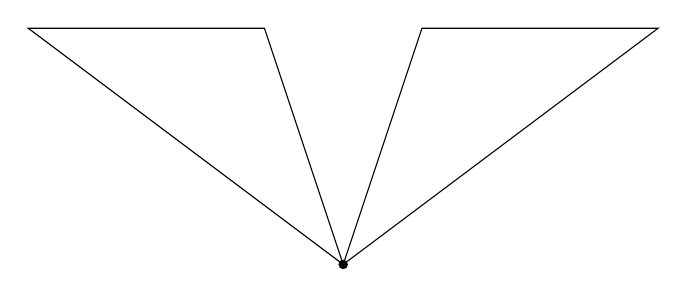
\begin{tikzpicture}
  [anchor=base]
  \draw (0,0) -- (4,3) -- (1,3) -- cycle;
  \draw (0,0) -- (-4,3) -- (-1,3) -- cycle;
  \fill (0,0) circle (0.06);
\end{tikzpicture}
\caption{Strict sum of pointed cpos}
\label{fig:holcf-strict-sum}
\end{figure}

In \HOLCF{11}, we define the strict sum of \isa{'a} and \isa{'b} as a set of triples of type \isa{(tr \<times> 'a \<times> 'b)}. The first component is a tag specifying whether the value should be interpreted as a left- or right-injection. Depending on the value of the tag, the injected value is stored in either the second or third slot, with the other slot containing \isa{\<bottom>}. The bottom element of the strict sum type is represented as \isa{\<bottom> = (\<bottom>, \<bottom>, \<bottom>)}.

\begin{isacode}
pcpodef ('a, 'b) ssum (infixr "++" 10) = 
  "{p :: (tr \<times> 'a::pcpo \<times> 'b::pcpo). p = \<bottom> \<or>
      (fst p = TT \<and> fst (snd p) \<noteq> \<bottom> \<and> snd (snd p) = \<bottom>) \<or>
      (fst p = FF \<and> fst (snd p) = \<bottom> \<and> snd (snd p) \<noteq> \<bottom>) }"
\end{isacode}

\noindent
The proof obligations for \isa{pcpodef} are that the set contains \isa{UU}, and set membership is admissible. As with the strict product, both goals are solved immediately by simplification. For the strict sum type, the \textsc{Cpodef} package provides a set of theorems just like the ones shown in Fig.~\ref{fig:holcf-sprod-pcpodef} for strict product; we omit the strict sum versions here.

\paragraph{Constructor functions.} After defining the type, we can define the constructor functions \isa{sinl} and \isa{sinr}.\footnote{The names of \isa{sinl} and \isa{sinr} come from earlier versions of LCF; respectively they stand for ``\emph{s}trict-\emph{in}jection-\emph{l}eft'' and ``\emph{s}trict-\emph{in}jection-\emph{r}ight''.} Because both constructor functions are supposed to be strict, we use the \isa{seq} operator to ensure that the tag component is \isa{UU} whenever the constructor argument is \isa{UU}.

\indexdef{sinl}
\begin{isacode}
definition sinl :: "'a -> ('a ++ 'b)"
  where "sinl = (\<Lambda> a. Abs_ssum (seq`a`TT, a, \<bottom>))"
\end{isacode}
\unmedskip
\indexdef{sinr}
\begin{isacode}
definition sinr :: "'b -> ('a ++ 'b)"
  where "sinr = (\<Lambda> b. Abs_ssum (seq`b`FF, \<bottom>, b))"
\end{isacode}

Similarly to the strict product, the next thing we must do is prove how \isa{Rep_ssum} acts on the constructors. After proving lemmas to the effect that \isa{(seq`a`TT, a, \<bottom>)} and \isa{(seq`b`FF, \<bottom>, b)} are always in the set \isa{ssum}, we can use \isa{cont_Abs_ssum} and \isa{Abs_ssum_inverse} to derive the following two rules.

\indexthm{Rep_ssum_sinl}
\indexthm{Rep_ssum_sinr}
\begin{isacodes}
lemma Rep_ssum_sinl: "Rep_ssum (sinl`a) = (seq`a`TT, a, \<bottom>)"
lemma Rep_ssum_sinr: "Rep_ssum (sinr`b) = (seq`b`FF, \<bottom>, b)"
\end{isacodes}

\noindent
These are combined with other lemmas about \isa{Rep_ssum} to form \indexthm{Rep_ssum_simps}\isa{Rep_ssum_simps}, which is the strict-sum analog of \isa{Rep_sprod_simps} from the previous section. This set of rewrite rules lets us reduce comparisons on type \isa{'a ++ 'b} to comparisons on types \isa{tr}, \isa{'a} and \isa{'b}. We can use them (together with \isa{seq_conv_if}, as needed) to prove the complete set of simplification rules for \isa{sinl} and \isa{sinr} shown in Fig.~\ref{fig:holcf-sinl-sinr}.

\begin{figure}
\indexthm{sinl_below}
\indexthm{sinr_below}
\indexthm{sinl_below_sinr}
\indexthm{sinr_below_sinl}
\begin{minipage}{0.275\linewidth}
\begin{isabelle}
lemma sinl_below
lemma sinr_below
lemma sinl_below_sinr
lemma sinr_below_sinl
\end{isabelle}
\end{minipage}
\begin{minipage}{0.7\linewidth}
\begin{isabelle}
[simp]: "(sinl`x \<sqsubseteq> sinl`y) = (x \<sqsubseteq> y)"
[simp]: "(sinr`x \<sqsubseteq> sinr`y) = (x \<sqsubseteq> y)"
[simp]: "(sinl`x \<sqsubseteq> sinr`y) = (x = \<bottom>)"
[simp]: "(sinr`x \<sqsubseteq> sinl`y) = (x = \<bottom>)"
\end{isabelle}
\end{minipage}

\indexthm{sinl_eq}
\indexthm{sinr_eq}
\indexthm{sinl_eq_sinr}
\indexthm{sinr_eq_sinl}
\begin{minipage}{0.275\linewidth}
\begin{isabelle}
lemma sinl_eq
lemma sinr_eq
lemma sinl_eq_sinr
lemma sinr_eq_sinl
\end{isabelle}
\end{minipage}
\begin{minipage}{0.7\linewidth}
\begin{isabelle}
[simp]: "(sinl`x = sinl`y) = (x = y)"
[simp]: "(sinr`x = sinr`y) = (x = y)"
[simp]: "(sinl`x = sinr`y) = (x = \<bottom> \<and> y = \<bottom>)"
[simp]: "(sinr`x = sinl`y) = (x = \<bottom> \<and> y = \<bottom>)"
\end{isabelle}
\end{minipage}

\indexthm{sinl_strict}
\indexthm{sinr_strict}
\indexthm{sinl_bottom_iff}
\indexthm{sinr_bottom_iff}
\begin{minipage}{0.275\linewidth}
\begin{isabelle}
lemma sinl_strict
lemma sinr_strict
lemma sinl_bottom_iff
lemma sinr_bottom_iff
\end{isabelle}
\end{minipage}
\begin{minipage}{0.7\linewidth}
\begin{isabelle}
[simp]: "sinl`\<bottom> = \<bottom>"
[simp]: "sinr`\<bottom> = \<bottom>"
[simp]: "(sinl`x = \<bottom>) = (x = \<bottom>)"
[simp]: "(sinr`x = \<bottom>) = (x = \<bottom>)"
\end{isabelle}
\end{minipage}
\caption{Order, injectivity, distinctness, and strictness of \isa{sinl} and \isa{sinr}}
\label{fig:holcf-sinl-sinr}
\end{figure}
 
The same rewrites are also sufficient to prove the case analysis rule for the strict sum type. Starting with the fact \isa{Rep_ssum y \<in> ssum} (a theorem provided by \textsc{Cpodef}), we can unfold the definition of \isa{ssum} and then use \isa{Rep_ssum_simps} with the \isa{auto} tactic to complete the proof.

\indexthm{ssumE}
\begin{isacode}
lemma ssumE: "[|y = UU ==> P;
  !!a. [|y = sinl`a; a ~= UU|] ==> P; !!b. [|y = sinr`b; b ~= UU|] ==> P|] ==> P"
\end{isacode}

\noindent
The induction rule for strict sums is a direct consequence of the case analysis rule.

\indexthm{ssum_induct}
\begin{isacode}
lemma ssum_induct:
  "[|P UU; !!a. a ~= UU ==> P (sinl`a); !!b. b ~= UU ==> P (sinr`b)|] ==> P x"
\end{isacode}

We can prove if-and-only-if compactness rules for \isa{sinl} and \isa{sinr}. For the ($\Longleftarrow$) direction, we use a compactness rule provided by \textsc{Cpodef}: A value of type \isa{'a \<oplus> 'b} is compact if its representation in type \isa{tr \<times> 'a \<times> 'b} is compact. The proof of the ($\Longrightarrow$) direction uses the definition of compactness and the \isa{adm_subst} rule. We assume \isa{compact (sinl`a)}, which means \isa{adm (\<lambda>x. sinl`a \<notsqsubseteq> x)}; this implies \isa{adm (\<lambda>x. sinl`a \<notsqsubseteq> sinl`x)}, which simplifies to \isa{adm (\<lambda>x. a \<notsqsubseteq> x)}, which is the definition of \isa{compact a}. The proof for \isa{sinr} is identical.

\indexthm{compact_sinl_iff}
\indexthm{compact_sinr_iff}
\begin{isacodes}
lemma compact_sinl_iff [simp]: "compact (sinl`a) = compact a"
lemma compact_sinr_iff [simp]: "compact (sinr`b) = compact b"
\end{isacodes}
\unmedskip

\paragraph{Case combinator.} Besides the constructors \isa{sinl} and \isa{sinr}, the other basic operation on strict sums is the case combinator, \isa{sscase}. The definition uses \isa{Rep_ssum} to examine its argument, and the continuous if-then-else operation on type \isa{tr} to select which branch to take.
\indexdef{sscase}
\begin{isacode}
definition sscase :: "('a -> 'c) -> ('b -> 'c) -> ('a ++ 'b) -> 'c"
  where "sscase = (\<Lambda> f g s. (\<lambda>(t, x, y). If t then f`x else g`y) (Rep_ssum s))"
\end{isacode}
Using lemma \isa{cont_Rep_ssum} from the \textsc{Cpodef} package, it is easy to show that the abstractions used in the definition of \isa{sscase} are continuous. Proving the characteristic properties of \isa{sscase} is a simple matter of beta-reducing the definition and simplifying with \isa{Rep_ssum_simps}.
\indexthm{sscase_simps}
\begin{isacode}
lemma sscase_simps [simp]:
  "sscase`f`g`\<bottom> = \<bottom>"
  "x \<noteq> \<bottom> ==> sscase`f`g`(sinl`x) = f`x"
  "y \<noteq> \<bottom> ==> sscase`f`g`(sinr`y) = g`y"
\end{isacode}
As with the other case combinators, we define special syntax for \isa{sscase}. The term \isa{sscase`(\<Lambda> a. t)`(\<Lambda> b. u)`x} is rendered as \isa{(case x of sinl`a => t | sinr`b => u)}.


%%%%%%%%%%%%%%%%%%%%%%%%%%%%%%%%%%%%%%%%%%%%%%%%%%%%%%%%%%%%%%%%%%%%%%

\section{Automating continuity proofs}
\label{sec:holcf-automation}

When reasoning in HOLCF, continuity goals pop up all the time: Every beta-reduction of a continuous function abstraction requires a continuity proof. Continuity proofs are also needed, for example, to show admissibility of predicates like \isa{(\<lambda>x. f x << g x)}. Because they occur so often in practice, it is important that continuity proofs be both automatic and efficient---they should involve a minimal number of proof steps, and be processed in a short amount of time.

In this section we discuss three alternative proof techniques for continuity, starting with the method used by previous versions of HOLCF. Following this, we introduce two novel proof methods for continuity, each of which offers improved efficiency in terms of number of proof steps and running time.

\subsection{Original HOLCF continuity tactic}

\HOLCF{95} introduced a continuity tactic that repeatedly applied the following four continuity lemmas:

\indexthm{cont_id}
\begin{isacode}
lemma cont_id: "cont (\<lambda>x. x)"
\end{isacode}
\unmedskip
\indexthm{cont_const}
\begin{isacode}
lemma cont_const: "cont (\<lambda>x. c)"
\end{isacode}
\unmedskip
\indexthm{cont2cont_APP}
\begin{isacode}
lemma cont2cont_APP:
  "[|cont (\<lambda>x. f x); cont (\<lambda>x. t x)|] ==> cont (\<lambda>x. (f x)`(t x))"
\end{isacode}
\unmedskip
\indexthm{cont2cont_LAM}
\begin{isacode}
lemma cont2cont_LAM:
  "[|\<And>x. cont (\<lambda>y. f x y); \<And>y. cont (\<lambda>x. f x y)|] ==> cont (\<lambda>x. \<Lambda> y. f x y)"
\end{isacode}

If we add these four rules to the simplifier, then we will be able to prove continuity automatically for any term written in the LCF sub-language---i.e., any term consisting of continuous applications, continuous abstractions, and variables and constants with continuous function types. Looking at the forms of the rules, we can see that the terms in the assumptions are all strictly smaller than the terms in the conclusions, showing that the process of applying rules must eventually terminate.

But while the proofs may be automatic, they are not efficient. The problem lies specifically with the rule \isa{cont2cont_LAM}. Consider what happens when we have a term with multiple nested function abstractions (see Fig.~\ref{fig:holcf-cont-slow}). After repeatedly applying rule \isa{cont2cont_LAM} as many times as possible, we are left with \emph{eight} subgoals. In fact, the number of subgoals is equal to $2^n$, where $n$ is the number of nested lambdas.

\begin{figure}
\begin{singlespace}
\begin{isabelle}
lemma "cont (%x. \<Lambda> a b c. f`a`b`c`x)"
  apply (intro cont2cont_LAM)

 goal (8 subgoals):
 1. !!x a b. cont (%c. f`a`b`c`x)
 2. !!x a c. cont (%b. f`a`b`c`x)
 3. !!x b a. cont (%c. f`a`b`c`x)
 4. !!x b c. cont (%a. f`a`b`c`x)
 5. !!a x b. cont (%c. f`a`b`c`x)
 6. !!a x c. cont (%b. f`a`b`c`x)
 7. !!a b x. cont (%c. f`a`b`c`x)
 8. !!a b c. cont (%x. f`a`b`c`x)
\end{isabelle}
\end{singlespace}
\caption{Exponential blow-up using rule \isa{cont2cont_LAM}}
\label{fig:holcf-cont-slow}
\end{figure}

However, it is immediately evident that many of these subgoals are really the same; there are only $(n+1)$ distinct subgoals, each requiring continuity with respect to a different variable. This suggests the possibility of solving continuity goals in less than an exponential number of steps.

\subsection{Bottom-up continuity proofs}

One possible strategy is to work bottom-up: First prove continuity for the small subterms, and then combine those proofs to get continuity over the larger terms. Note that this is basically opposite to the introduction-rules approach, which works top-down. For each subterm, we construct a list of continuity theorems, one for each bound variable that occurs free in the subterm. For example, when proving \isa{cont (\<lambda>x. \<Lambda> a b c. f`a`b`c`x)}, the subterm \isa{(\<Lambda> c. f`a`b`c`x)} will have continuity theorems for the variables \isa{a}, \isa{b} and \isa{x} (shown in Fig.~\ref{fig:holcf-cont-algorithm} as \isa{a5}, \isa{b5}, and \isa{x5}). We treat \isa{f} like a constant, because it is free in the original goal.

\begin{figure}
\begin{singlespace}
\begin{isabelle}
have a0: "cont (%a. a)" by (rule cont_id)
from cont_const a0 have a1: "cont (%a. f`a)" by (rule cont2cont_APP)
from a1 cont_const have a2: "!!b. cont (%a. f`a`b)" by (rule cont2cont_APP)

...

from ... have a4: "!!b c x. cont (%a. f`a`b`c`x)" by (rule cont2cont_APP)
from ... have b4: "!!a c x. cont (%b. f`a`b`c`x)" by (rule cont2cont_APP)
from ... have c4: "!!a b x. cont (%c. f`a`b`c`x)" by (rule cont2cont_APP)
from ... have x4: "!!a b c. cont (%x. f`a`b`c`x)" by (rule cont2cont_APP)

from c4 and a4 have a5: "!!b x. cont (%a. \<Lambda> c. f`a`b`c`x)" by (rule cont2cont_LAM)
from c4 and b4 have b5: "!!a x. cont (%b. \<Lambda> c. f`a`b`c`x)" by (rule cont2cont_LAM)
from c4 and x4 have x5: "!!a b. cont (%x. \<Lambda> c. f`a`b`c`x)" by (rule cont2cont_LAM)
 
from b5 and a5 have a6: "!!x. cont (%a. \<Lambda> b c. f`a`b`c`x)" by (rule cont2cont_LAM)
from b5 and x5 have x6: "!!a. cont (%x. \<Lambda> b c. f`a`b`c`x)" by (rule cont2cont_LAM)

from a6 and x6 have x7: "cont (%x. \<Lambda> a b c. f`a`b`c`x)" by (rule cont2cont_LAM)
\end{isabelle}
\end{singlespace}
\caption{Bottom-up algorithm for proving continuity, using forward proof}
\label{fig:holcf-cont-algorithm}
\end{figure}

Next we move up to the next larger subterm, \isa{(\<Lambda> b c. f`a`b`c`x)}, which gets continuity theorems for the variables \isa{a} and \isa{x} (shown as \isa{a6} and \isa{x6}). Each of the new continuity theorems is derived from two earlier ones using the rule \isa{cont2cont_LAM}. Note that rule \isa{b5} is used more than once; such re-use prevents the exponential blow-up that we had before.

The bottom-up algorithm is now implemented in \HOLCF{11} (\texttt{HOLCF/Tools{\slash}cont\_proc.ML}). It has the advantage of being fast: It solves continuity subgoals using a small number of rule applications (quadratic in the number of nested lambdas, rather than exponential). Another advantage is that without any extra work, the algorithm can return a whole list of continuity theorems that it proved for subterms. This is useful for doing multiple beta-reductions, for example when proving something like \isa{(\<Lambda> a b c. f`a`b`c`x)`u`v`w = f`u`v`w`x}. This technique is used successfully by the \textsc{Domain} package for internal proofs, where large subgoals of this form arise from large datatype definitions (see Sec.~\ref{sec:domain-implementation}).

Compared to using introduction rules, the main disadvantage of the bottom-up algorithm is that it is difficult to extend the system to handle new constants. For example, when M\"{u}ller introduced the \isa{lift} type to allow mixing HOL and LCF terms, he was able to extend the continuity tactic by simply adding a couple of new rules, such as the one below for \isa{lift_case} \cite[\S5.2.2]{mueller98thesis} \cite[\S4.3.2]{hol+lcf}.
%
\indexthm{cont2cont_lift_case}
\begin{isacode}
lemma cont2cont_lift_case:
  "[|!!y. cont (\<lambda>x. f x y); cont (\<lambda>x. g x)|]
    ==> cont (\<lambda>x. case g x of \<bottom> => \<bottom> | Def y => f x y)"
\end{isacode}
%
Similarly, we have continuity rules for operations on the HOL product type:
%
\indexthm{cont2cont_Pair}
\begin{isacode}
lemma cont2cont_Pair:
  "[|cont (\<lambda>x. f x); cont (\<lambda>x. g x)|] ==> cont (\<lambda>x. (f x, g x))"
\end{isacode}
\unmedskip
\indexthm{cont2cont_prod_case}
\begin{isacode}
lemma cont2cont_prod_case:
  "[|!!a b. cont (\<lambda>x. f x a b); !!x b. cont (\<lambda>a. f x a b);
    !!x a. cont (\<lambda>b. f x a b); cont (\<lambda>x. g x)|]
    ==> cont (\<lambda>x. case g x of (a, b) => f x a b)"
\end{isacode}
%
An ideal continuity prover should allow users to add support for new constants by adding such rules. But as implemented, the bottom-up continuity algorithm is not so easily extensible. Properly supporting rules like \isa{cont2cont_prod_case} is especially troublesome because, like \isa{cont2cont_LAM}, it has multiple hypotheses for the same subterm, and would require similar handling to avoid an exponential blow-up. Yet the rule has a different form than \isa{cont2cont_LAM}. A single algorithm that could handle the full range of possibilities for such rules would have to be rather sophisticated.

\subsection{Efficient continuity rules using products}

As it turns out, it is possible to design an extensible set of continuity introduction rules that avoids the exponential blow-up inherent in the original \HOLCF{95} continuity tactic. The key to designing these rules is a property of continuous functions $f : D \times E \to F$. It is a standard result in domain theory that a function on a product type is continuous if and only if it is continuous in each component separately \cite[Lemma 3.2.6]{abramsky94domain}. This property is formalized in the \HOLCF{11} theory of products as lemma \isa{prod_cont_iff}.
%
\indexthm{prod_cont_iff}
\begin{isacode}
lemma prod_cont_iff:
  "cont f <-> (\<forall>y. cont (\<lambda>x. f (x, y))) \<and> (\<forall>x. cont (\<lambda>y. f (x, y)))"
\end{isacode}
%
We can use this theorem to combine the two premises of the \isa{cont2cont_LAM} rule into one. Compare the two versions of this rule:
%
\indexthm{cont2cont_LAM}
\begin{isacode}
lemma cont2cont_LAM:
  "[|\<And>x. cont (\<lambda>y. f x y); \<And>y. cont (\<lambda>x. f x y)|] ==> cont (\<lambda>x. \<Lambda> y. f x y)"
\end{isacode}
\unmedskip
\indexthm{cont2cont_LAM'}
\begin{isacode}
lemma cont2cont_LAM':
  "cont (\<lambda>p. f (fst p) (snd p)) ==> cont (\<lambda>x. \<Lambda> y. f x y)"
\end{isacode}
%
We can evaluate the behavior of the new \isa{cont2cont_LAM'} rule by considering the same continuity goal we used before in Fig.~\ref{fig:holcf-cont-slow}. After applying the continuity rule \isa{cont2cont_LAM'} three times, we are now left with just a single subgoal (see Fig.~\ref{fig:holcf-cont-fast}). The remaining goal can be solved by applying standard continuity rules (\isa{cont_id}, \isa{cont_const}, and \isa{cont2cont_APP}) together with continuity rules for \isa{fst} and \isa{snd}. The complete set of rules (which we call \isa{cont2cont} rules) for proving continuity of LCF terms is shown in Fig.~\ref{fig:holcf-cont2cont-rules}. All of them are safe to add to the Isabelle simplifier.

\begin{figure}
\begin{singlespace}
\begin{isabelle}
lemma "cont (%x. \<Lambda> a b c. f`a`b`c`x)"
  apply (intro cont2cont_LAM')
 
goal (1 subgoal):
 1. cont (%p. f`(snd (fst (fst p)))`(snd (fst p))`(snd p)`(fst (fst (fst p))))
\end{isabelle}
\end{singlespace}
\caption{Efficient behavior of continuity introduction rule \isa{cont2cont_LAM'}}
\label{fig:holcf-cont-fast}
\end{figure}

\begin{figure}
\begin{isacode}
lemma cont_id [simp]: "cont (\<lambda>x. x)"
\end{isacode}
\unmedskip
\begin{isacode}
lemma cont_const [simp]: "cont (\<lambda>x. c)"
\end{isacode}
\unmedskip
\begin{isacode}
lemma cont2cont_fst [simp]: "cont (%x. f x) ==> cont (%x. fst (f x))"
\end{isacode}
\unmedskip
\begin{isacode}
lemma cont2cont_snd [simp]: "cont (%x. f x) ==> cont (%x. snd (f x))"
\end{isacode}
\unmedskip
\begin{isacode}
lemma cont2cont_APP [simp]:
  "[|cont (\<lambda>x. f x); cont (\<lambda>x. t x)|] ==> cont (\<lambda>x. (f x)`(t x))"
\end{isacode}
\unmedskip
\begin{isacode}
lemma cont2cont_LAM' [simp]:
  "cont (\<lambda>p. f (fst p) (snd p)) ==> cont (\<lambda>x. \<Lambda> y. f x y)"
\end{isacode}
\caption{Complete set of efficient \isa{cont2cont} rules for LCF terms}
\label{fig:holcf-cont2cont-rules}
\end{figure}

Unlike rule \isa{cont2cont_LAM}, each rule in Fig.~\ref{fig:holcf-cont2cont-rules} has only one continuity premise for each subterm. Proving continuity with this set of rules requires more than a linear number of steps, though, because as lambdas are eliminated, the subgoal grows to a larger size: \isa{fst} and \isa{snd} are introduced on every bound variable. But the size increase is not exponential; it is merely quadratic in the number of nested lambdas. So, like the bottom-up algorithm, the \isa{cont2cont} rules can discharge a continuity goal with nested lambdas in a quadratic number of steps. In practice, the run-time efficiency of the \isa{cont2cont} rules is about the same as for the bottom-up continuity tactic. (Either can discharge a continuity goal with twenty nested lambdas in a fraction of a second, and the total run-time for each seems to be $O(n^3)$.)

The \isa{cont2cont} rules are easily extensible. We can add new rules to the simplifier for each new constant we want (such as \isa{cont2cont_lift_case}) without any trouble. For constants like \isa{prod_case}, whose continuity rules require continuity of multiple variables over the same subterm, we can use \isa{prod_cont_iff} to derive an efficient version of the rule, just like we did for \isa{cont2cont_LAM}. For example, here is the efficient \isa{cont2cont} rule for \isa{prod_case}:

\indexthm{cont2cont_prod_case'}
\begin{isacode}
lemma cont2cont_prod_case' [simp]:
  "[|cont (%p. f (fst p) (fst (snd p)) (snd (snd p))); cont (%x. g x)|]
    ==> cont (%x. case g x of (a, b) => f x a b)"
\end{isacode}

For organizing continuity introduction rules, \HOLCF{11} provides a special \isa{cont2cont} theorem attribute. Declaring a lemma with \isa{[cont2cont]} dynamically adds it to a list of theorems, which is also referred to by the name \isa{cont2cont}. (Typically each \isa{cont2cont} rule should also be added to the simplifier.) Users can then do continuity proofs with the proof method ``\isa{intro cont2cont}''.

Using ``\isa{intro cont2cont}'' is a bit faster (by about a factor of two) than calling ``\isa{simp}'' on a continuity goal, because it has a smaller, targeted set of rules, and avoids deep recursive calls to the simplifier. To take advantage of this speedup in the common case, \HOLCF{11} defines a special simplification procedure (or ``simproc'') for the beta reduction rule:

\indexthm{beta_cfun}
\begin{isacode}
lemma beta_cfun: "cont f ==> (\<Lambda> x. f x)`u = f u"
\end{isacode}

\noindent
In \HOLCF{11}, \isa{beta_cfun} is not declared with the \isa{[simp]} attribute. Instead, the simplifier is configured to call a certain simproc when it sees a term matching the pattern \isa{(\<Lambda> x. f x)`u}. When the simproc is run, it tries to prove the goal \isa{cont f} using the proof method ``\isa{intro cont2cont}''. If the subproof succeeds, the simproc returns the unconditional equation \isa{(\<Lambda> x. f x)`u = f u}; if the subproof fails, then the simproc returns the ordinary conditional rule, which will then cause the simplifier to attempt to solve the side-condition \isa{cont f} by calling itself recursively.

A nice feature of this setup is that users do not have to know anything about the \isa{cont2cont} attribute; if a user proves a continuity rule for a new constant, and declares it with \isa{[simp]}, then it will work with the other existing \isa{cont2cont} rules as expected. Declaring the same rule with \isa{[cont2cont]} is optional, and will not affect the set of provable continuity goals; the only effect is that the same continuity goals will be proved more quickly when doing beta reduction.

%%%%%%%%%%%%%%%%%%%%%%%%%%%%%%%%%%%%%%%%%%%%%%%%%%%%%%%%%%%%%%%%%%%%%%

\section{Evaluation}
\label{sec:holcf-evaluation}

This chapter has described the core of the \HOLCF{11} libraries, consisting of the type class hierarchy, various notions of domain theory such as continuity and admissibility, and the definition of all the basic HOLCF types.

The material presented in this chapter was mostly present in some form or other in Regensburger's original \HOLCF{95} \cite{regensburger94thesis, regensburger95holcf}. However, the new \HOLCF{11} offers various improvements over the original. The primary novel contributions of this work are threefold: the \textsc{Cpodef} package, the improved automation for continuity proofs, and the use of compactness for proving admissibility.

\paragraph{Cpodef.} The \textsc{Cpodef} package provides a very convenient, streamlined way to define new types in \HOLCF{11}. Using the \textsc{Cpodef} package can result it a big reduction in the size and complexity of proof scripts. For example, in \HOLCF{99}, the theory of strict products comprised over 900 lines of definitions and proof scripts; after converting the theory to use the \textsc{Cpodef} package, this was reduced to less than 200 lines of code. Similarly, defining the strict sum type with \textsc{Cpodef} reduced that theory file from over 1300 lines to less than 300.

Of all the \HOLCF{11} types \emph{not} defined with \textsc{Cpodef}, the lifted cpo type \isa{'a u} is the one with the most difficult cpo instance proofs. Unfortunately it seems that no suitable cpo exists from which \isa{'a u} could be defined as a subtype, although there is one that comes close:

\begin{isacode}
pcpodef 'a u2 = "{p::one \<times> 'a. p = \<bottom> \<or> fst p = ONE}"
\end{isacode}

\noindent
The above definition only works if type \isa{'a} is already pointed, however; in contrast, the currently implemented definition works for any \isa{'a} in class \isa{cpo}.

\paragraph{Continuity proofs.} The original Edinburgh LCF and Cambridge LCF systems \cite{GMW79, paulson87lcf} did not require proofs of continuity, because reasoning was done \emph{in} the LCF logic, which does not have an explicit concept of continuous functions. In contrast, using HOLCF means reasoning \emph{about} LCF terms and formulas, \emph{in} higher-order logic. Because higher-order logic can express non-continuous functions that are not expressible in LCF, systems like HOLCF that model LCF in higher-order logic must reason explicitly about continuity.

The \HOLCF{95} continuity tactic could prove the continuity of any function corresponding to an LCF term. However, for some terms the tactic was prohibitively slow: On nested lambda-abstractions like \isa{(\<lambda>x. \<Lambda> y. e x y)}, the tactic would prove continuity of the body twice, once for each variable. Each additional lambda-abstraction would double the amount of work required, leading to an exponential running time.

\HOLCF{95} was not the only formalization of LCF to suffer from this problem. The HOL-CPO system by Sten Agerholm \cite{agerholm94thesis} is another formalization of LCF in higher-order logic (though implemented in a different theorem prover), released contemporaneously with the original \HOLCF{95}. In HOL-CPO, continuous function types are represented as subsets of a full function type. Continuity proofs are performed by a ``type-checker'', which proves that a given function is an element of a particular continuous function type. For abstractions of the form \isa{(\<lambda>x. \<lambda>y. e x y)}, the type-checker traverses the body twice, proving continuity separately in \isa{x} and \isa{y} \cite[\S5.2.2]{agerholm94thesis}. In other words, it works just like the \HOLCF{95} continuity tactic: Deeply nested abstractions would cause the same exponential run-time behavior.

The HOL-CPO system does provide a potential workaround: It defines combinators like \isa{curry f = (\<lambda>x y. f (x, y))}, with which users can write multi-argument functions without using nested lambdas. For example, the three-argument function \isa{(\<lambda>x y z. e[x, y, z])} could be written instead as \isa{curry (curry (\<lambda>p. e[fst (fst p), snd} \isa{(fst p), snd p]))}. Using \isa{curry} permits continuity proofs with the efficiency of the \HOLCF{11} \isa{cont2cont} rules, at the expense of being more cumbersome to use.

The improved automation for continuity makes \HOLCF{11} useful for reasoning about a larger set of programs. In particular, it is now practical to reason about functions with a large number of arguments. For example, beta-reducing a function of a dozen arguments with the old continuity tactic could easily take a minute or more; the new continuity rules can reduce the same function in a fraction of a second. A faster continuity checker also makes larger datatype definitions more practical, because the \textsc{Domain} package performs many beta-reductions in its internal proofs.

\paragraph{Admissibility proofs.} In Cambridge LCF, admissibility was not actually formalized in the logic. Rather, fixed point induction was accompanied by a hard-coded syntactic admissibility test \cite[page 200]{paulson87lcf}. The test examined both the structure of the formula, and also the chain-finiteness of the types involved. For example, in LCF the predicate \isa{(\<lambda>x. f x \<sqsubseteq> y --> g x = h x)} would always pass the admissibility test, while \isa{(\<lambda>x. f x = y --> g x = h x)} would pass only if either \isa{x} or \isa{y} had a chain-finite type. The earlier Edinburgh LCF used a similar test \cite[page 77]{GMW79}.

\HOLCF{99} included some proof automation for admissibility, with roughly the same capabilities as the hard-coded check in Cambridge LCF. The automation comprised a set of structural rules for various connectives, plus a special admissibility tactic that considered chain-finiteness \cite{hol+lcf, mueller98thesis}. The structural rules included all those in Fig.~\ref{fig:holcf-adm-simps}, plus the rule \isa{"cont t ==> adm (\<lambda>x. t x ~= \<bottom>)"}. (No rules involving compactness were present, as \HOLCF{99} did not have a notion of compactness.) After applying the structural rules, the admissibility tactic would try to solve any remaining subgoals using \isa{adm_subst} and \isa{adm_chfin}.

\begin{isacodes}
lemma adm_subst: "[|cont f; adm P|] ==> adm (\<lambda>x. P (f x))"
lemma adm_chfin [simp]: "adm (\<lambda>(x::'a::chfin). P x)"
\end{isacodes}

\noindent
For example, on the goal \isa{adm (\<lambda>x. f`x = TT --> g`x = h`x)}, applying the structural rules would leave the subgoal \isa{adm (\<lambda>x. f`x ~= TT)}. Then the tactic would apply \isa{adm_subst}, leaving the goals \isa{adm (\<lambda>y. y ~= TT)} (an instance of \isa{adm_chfin}, because \isa{tr} is chain-finite) and \isa{cont (\<lambda>x. f`x)} (solvable by the continuity tactic).

Agerholm's HOL-CPO also includes a prover for admissibility (he calls it ``inclusiveness'') with capabilities similar to the \HOLCF{99} tactic \cite[\S5.3]{agerholm94thesis}.
 
The limitations of the \HOLCF{99} admissibillity tactic were noted by M\"uller with regards to his formalization of I/O automata \cite[\S10.3.2]{mueller98thesis}. One of the proof scripts in that formalization\footnote{M\"uller's formalization is included with the Isabelle distribution, in the \texttt{HOLCF/IOA} directory.} requires admissibility of the predicate \isa{(\<lambda>x. f`x ~=} \isa{nil)}, where \isa{nil} is a constructor for a recursive list type that is not chain-finite. When the proof script was written, no applicable lemmas were available to assist with a proof of admissibility; M\"uller resorted to declaring an axiom (no doubt with the intention that it be temporary!) rather than unfolding the definition and attempting a manual proof. In \HOLCF{11}, with the new compactness rules for admissibility in place, the same admissibility goal is solved automatically by the simplifier.

In \HOLCF{11}, the sophisticated \HOLCF{99} tactic for proving admissibility with \isa{adm_subst} and \isa{adm_chfin} has been discontinued, because it is no longer necessary. In practice, it was nearly always used in situations where one of the lemmas \isa{adm_compact_not_below}, \isa{adm_neq_compact}, or \isa{adm_compact_neq} from Fig.~\ref{fig:holcf-compact-simps} would now apply. These rules are strictly more powerful than the \HOLCF{99} admissibility tactic on such subgoals, because they are not limited to chain-finite types.

\chapter{Recursive Value Definitions: The Fixrec Package}
\label{ch:fixrec}

\section{Introduction}

In Haskell and most other functional programming languages, recursive definitions are supported directly: In the definition of a function, the constant being defined may occur freely on the right-hand side. This is in contrast to a theorem prover like Isabelle, whose primitive definitions are required to be non-recursive in order to guarantee logical soundness.

In Isabelle, a recursive specification of a new constant cannot be used directly as a definition. The specification must be used indirectly: First, the recursive specification must be somehow transformed into a \emph{non}-recursive definition of the constant. Second, this definition can then be used to prove the original specification as a theorem.

Isabelle/HOL already includes a number of packages that mechanize this kind of process for certain kinds of recursive definitions. The \textsc{Datatype} package provides the \isa{primrec} command for defining primitive-recursive functions over data\-types \cite{isabelle-tutorial}; the \textsc{Recdef} and \textsc{Function} packages define functions that use well-founded recursion \cite{Slind96recdef, Krauss10a}.

In \HOLCF{99}, no definition package for general recursive functions existed; such functions could only be defined by explicitly using the domain-theoretic fixed point combinator \isa{fix}. Users had to derive recursive equations manually, using the theory of least fixed points. This chapter introduces the {\fixrec} package for Isabelle/HOLCF, which automates this process: Users of \HOLCF{11} can now use {\fixrec} to formalize Haskell-style recursive function definitions directly.

\paragraph{Contributions.} The current implementation of \textsc{Fixrec} derives from the original version by Amber Telfer in 2004~\cite{Telfer04}. Since then, many new features have been added by the present author: The current version supports mutual recursion, and curried functions with any number of arguments. It also supports a wider class of patterns: Function definitions can use lazy or strict constructors, including constructors from Isabelle/HOL datatypes; definitions with overlapping patterns are also supported. The package is now suitable for verifying real Haskell programs: Some example case studies using \textsc{Fixrec}, including proofs by least fixed point induction, can be found in Chapter~\ref{ch:case-domain}.

\paragraph{Overview.} The remainder of this chapter starts by describing the features of the {\fixrec} package, from a user's point of view (\S\ref{sec:fixrec-features}). Then we establish an implementation strategy, showing how to translate lists of function equations into non-recursive definitions by expressing recursion with a fixed point combinator (\S\ref{sec:fixrec-fix}) and performing pattern match compilation (\S\ref{sec:fixrec-match}). Next are details of the actual implementation of the {\fixrec} package (\S\ref{sec:fixrec-impl}). Finally, we conclude with a comparison to related work, and directions for future work (\S\ref{sec:fixrec-conclusion}).

\section{Fixrec package features}
\label{sec:fixrec-features}

The {\fixrec} package lets users define recursive functions and values in HOLCF much like they can in Haskell or ML. Users can write function specifications with patterns, involving datatypes that may have been defined by the user. Users can use recursion freely within groups of simultaneously-defined values, with no need for termination proofs. The {\fixrec} package generates definitions for constants, proves each defining equation as a theorem, and also generates induction rules for reasoning about the new constants.

Patterns in \textsc{Fixrec} definitions can mention any of the constructors for basic HOLCF types (\S\ref{sec:holcf-types}): \isa{spair}, \isa{sinl}, \isa{sinr}, \isa{up}, \isa{ONE}, \isa{TT}, \isa{FF}, and also the \isa{Pair} constructor \isa{(_, _)} from Isabelle/HOL. Constructors for types defined by the \textsc{Domain} package are also supported, for instance \isa{LNil} and \isa{LCons} from the lazy list type below.
%
\indexdefx{domain 'a llist}
\indexdefx{LNil}
\indexdefx{LCons}
\begin{isacode}
domain 'a llist = LNil | LCons (lazy "'a") (lazy "'a llist")
\end{isacode}

The syntax for the \isa{fixrec} command is similar to other definition commands like \isa{primrec} or the \textsc{Function} package's \isa{fun} command. (A full syntax diagram is shown in Fig.~\ref{fig:fixrec-syntax}.) The equations must be separated by vertical bars; theorem names for each equation are optional.
%
\indexdefx{firsts}
\indexthmx{firsts_LNil}
\indexthmx{firsts_LCons}
\begin{isacode}
fixrec firsts :: "('a \<times> 'b) llist -> 'a llist"
  where firsts_LNil: "firsts`LNil = LNil"
  | firsts_LCons: "firsts`(LCons`(x, y)`xs) = LCons`x`(firsts`xs)"
\end{isacode}
%
The definition above generates the theorems \isa{firsts_LNil} and \isa{firsts_LCons}. It also declares a theorem list \isa{firsts.simps} consisting of all equations in the definition; these are added to the simplifier by default.

%%%%%%%%%%%%%%%%%%%%%%%%%%%%%%%%%%%%%%%%%%%%%%%%%%%%%%%%%%%%%%%%%%%%%%
\begin{figure}
\begin{center}
\begin{minipage}{0.625\linewidth}

\emph{definition}:

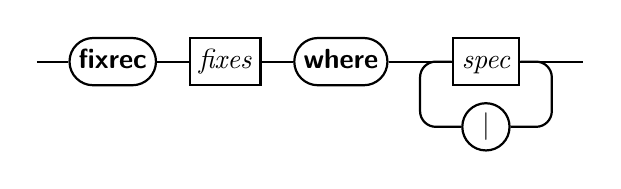
\begin{tikzpicture}
[ thick, draw, text height=1.5ex, text depth=0.4ex
, point/.style={coordinate}
, keyword/.style={rectangle, minimum size=6mm, rounded corners=3mm, draw, font=\bfseries\sffamily}
, terminal/.style={rectangle, minimum size=6mm, rounded corners=3mm, draw, font=\sffamily}
, nonterminal/.style={rectangle, minimum size=6mm, draw, font=\itshape}
, curve/.style={rounded corners=2mm}
]
\matrix[row sep=2mm, column sep=4mm] { 
% First row: 
\node (p0) [point] {}; &
\node (fixrec) [keyword] {fixrec}; & 
\node (fixes) [nonterminal] {fixes}; & 
\node (where) [keyword] {where}; & 
\node (p1) [point] {}; &
\node (spec) [nonterminal] {spec}; &
\node (p2) [point] {}; &
\node (p3) [point] {}; \\ 
% Second row: 
& & & & & \node (bar) [terminal] {\textbar}; & & \\ 
};
\draw [curve] (spec) -- (p2) |- (bar) -| (p1) -- (spec);
\draw [curve] (p0) -- (fixrec) -- (fixes) -- (where) -- (spec) -- (p3);
\end{tikzpicture}

\emph{fixes}:

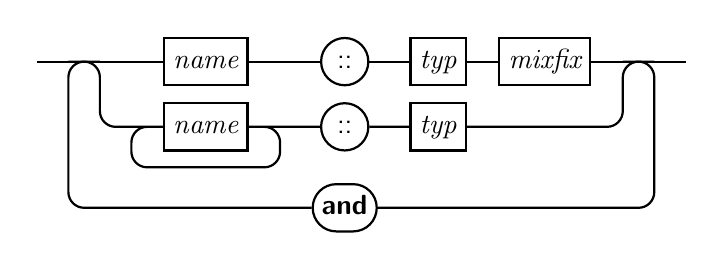
\begin{tikzpicture}
[ thick, draw, text height=1.5ex, text depth=0.4ex
, point/.style={coordinate}
, keyword/.style={rectangle, minimum size=6mm, rounded corners=3mm, draw, font=\bfseries\sffamily}
, terminal/.style={rectangle, minimum size=6mm, rounded corners=3mm, draw, font=\sffamily}
, nonterminal/.style={rectangle, minimum size=6mm, draw, font=\itshape}
, curve/.style={rounded corners=2mm}
]
\matrix[row sep=2mm, column sep=4mm] { 
% First row:
\node (p0) [point] {}; &
\node (p1) [point] {}; &
\node (p2) [point] {}; & &
\node (bind1) [nonterminal] {name}; & &
\node (colon1) [terminal] {::}; &
\node (typ1) [nonterminal] {typ}; &
\node (mixfix) [nonterminal] {mixfix}; &
\node (p3) [point] {}; &
\node (p4) [point] {}; &
\node (p5) [point] {}; \\
% Second row:
& & &
\node (p6) [point] {}; &
\node (bind2) [nonterminal] {name}; &
\node (p7) [point] {}; &
\node (colon2) [terminal] {::}; &
\node (typ2) [nonterminal] {typ}; \\
% Third row:
& & & &
\node (p8) [point] {}; \\
% Fourth row:
& & & & & &
\node (and) [keyword] {and}; \\
};
\draw [curve] (p0) -- (p1) -- (p2) -- (bind1) -- (colon1) -- (typ1) -- (mixfix) -- (p3) -- (p4) -- (p5);
\draw [curve] (p1) -- (p2) |- (bind2) -- (p7) |- (p8) -| (p6) -- (bind2) -- (colon2) -- (typ2) -| (p3) -- (p4);
\draw [curve] (p3) -- (p4) |- (and) -| (p1) -- (p2);
\end{tikzpicture}

\emph{spec}:

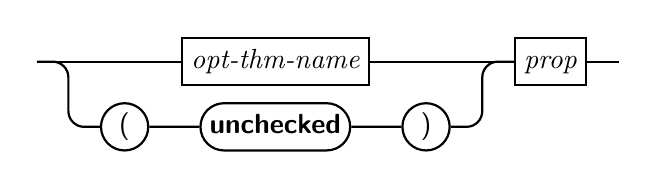
\begin{tikzpicture}
[ thick, draw, text height=1.5ex, text depth=0.4ex
, point/.style={coordinate}
, keyword/.style={rectangle, minimum size=6mm, rounded corners=3mm, draw, font=\bfseries\sffamily}
, terminal/.style={rectangle, minimum size=6mm, rounded corners=3mm, draw, font=\sffamily}
, nonterminal/.style={rectangle, minimum size=6mm, draw, font=\itshape}
, curve/.style={rounded corners=2mm}
]
\matrix[row sep=2mm, column sep=4mm] { 
% First row:
\node (p0) [point] {}; &
\node (p1) [point] {}; & &
\node (name) [nonterminal] {opt-thm-name}; & &
\node (p2) [point] {}; &
\node (prop) [nonterminal] {prop}; &
\node (p3) [point] {}; \\
% Second row:
& &
\node (lparen) [terminal] {(}; & 
\node (unchecked) [keyword] {unchecked}; & 
\node (rparen) [terminal] {)}; & & & \\
};
\draw [curve] (p0) -- (p1) -- (name) -- (p2) -- (prop) -- (p3);
\draw [curve] (p0) -- (p1) |- (lparen) -- (unchecked) -- (rparen) -| (p2) -- (prop);
\end{tikzpicture}

\emph{opt-thm-name}:

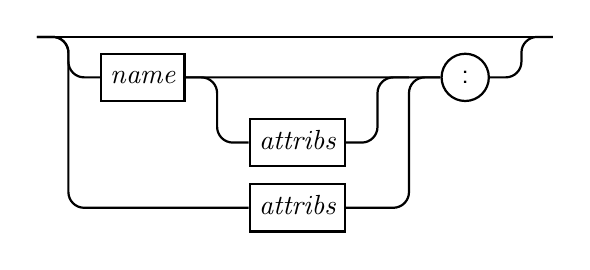
\begin{tikzpicture}
[ thick, draw, text height=1.5ex, text depth=0.4ex
, point/.style={coordinate}
, keyword/.style={rectangle, minimum size=6mm, rounded corners=3mm, draw, font=\bfseries\sffamily}
, terminal/.style={rectangle, minimum size=6mm, rounded corners=3mm, draw, font=\sffamily}
, nonterminal/.style={rectangle, minimum size=6mm, draw, font=\itshape}
, curve/.style={rounded corners=2mm}
]
\matrix[row sep=2mm, column sep=4mm] { 
% First row:
\node (p0) [point] {}; &
\node (p1) [point] {}; & & & & & & &
\node (p2) [point] {}; &
\node (p3) [point] {}; \\
% Second row:
& &
\node (name) [nonterminal] {name}; &
\node (p4) [point] {}; & &
\node (p5) [point] {}; &
\node (p6) [point] {}; &
\node (colon) [terminal] {:}; \\
% Third row:
& & & &
\node (attribs1) [nonterminal] {attribs}; \\
% Fourth row:
& & & &
\node (attribs2) [nonterminal] {attribs}; \\
};
\draw [curve] (p0) -- (p1) -- (p2) -- (p3);
\draw [curve] (p0) -- (p1) |- (name) -- (colon) -| (p2) -- (p3);
\draw [curve] (name) -- (p4) |- (attribs1) -| (p5) -- (p6);
\draw [curve] (p0) -- (p1) |- (attribs2) -| (p6) -- (colon);
\end{tikzpicture}

\end{minipage}
\end{center}

\caption{Input syntax for {\fixrec} package}
\label{fig:fixrec-syntax}
\end{figure}
%%%%%%%%%%%%%%%%%%%%%%%%%%%%%%%%%%%%%%%%%%%%%%%%%%%%%%%%%%%%%%%%%%%%%%

\paragraph{Lazy and strict constructors.} The {\fixrec} package works best with lazy constructor functions like \isa{LCons}, \isa{Pair} and \isa{up}. It also works with strict constructor functions, but definedness side conditions like \isa{x ~= \<bottom>} may be required.
%
\indexdefx{from_sinl}
\begin{isacode}
fixrec from_sinl :: "'a \<oplus> 'b -> 'a"
  where "x ~= \<bottom> ==> from_sinl`(sinl`x) = x"
\end{isacode}
%
If the side-condition in the above definition is omitted, the {\fixrec} package will not be able to prove the equation, and it will fail with an error message. Note that combinations of strict and lazy constructors can avoid the need for such side conditions.
%
\indexdefx{from_sinl_up}
\begin{isacode}
fixrec from_sinl_up :: "'a\<lifted> \<oplus> 'b -> 'a"
  where "from_sinl_up`(sinl`(up`x)) = x"
\end{isacode}
%
Even though \isa{sinl} is a strict constructor, the side condition \isa{up`x /= UU} is not needed. This is because \isa{up} is a lazy constructor and {\fixrec} can determine \isa{up`x /= UU} automatically.

\paragraph{Overlapping patterns.} The {\fixrec} package supports definitions with overlapping patterns. For example, consider the following function that zips two lists together: The first equation has specific patterns, while the second equation is a catch-all default case. The second equation cannot be proved as a theorem because it only applies when the first pattern fails.
%
\indexdefx{lzip}
\begin{isacode}
fixrec lzip :: "'a llist -> 'b llist -> ('a \<times> 'b) llist"
  where "lzip`(LCons`x`xs)`(LCons`y`ys) = LCons`(x, y)`(lzip`xs`ys)"
  | (unchecked) "lzip`xs`ys = LNil"
\end{isacode}
%
Usually {\fixrec} tries to prove all equations as theorems. The \isa{unchecked} option overrides this behavior, so {\fixrec} does not attempt to prove that particular equation. With the \isa{lzip} example, both equations influence the definition of \isa{lzip}, but only the first is proved as a theorem. The generated theorem list \isa{lzip.simps} then consists of only the first equation.

\paragraph{Generating extra equations.} The {\fixrec} package provides automation for proving extra equations beyond those included in the function definition. This takes the form of a proof method called \isa{fixrec_simp}. One use for \isa{fixrec_simp} is to prove specific rules for functions defined with overlapping patterns, like our earlier example \isa{lzip}.
%
\indexthmx{lzip_extra_simps}
\begin{isacode}
lemma lzip_extra_simps [simp]:
  shows "lzip`(LCons`x`xs)`LNil = LNil" and "lzip`LNil`ys = LNil"
  by fixrec_simp+
\end{isacode}
%
Another common use of the \isa{fixrec_simp} method is to prove strictness rules for functions.
%
\indexthmx{lzip_strict}
\begin{isacode}
lemma lzip_strict [simp]:
  shows "lzip`\<bottom>`ys = \<bottom>" and "lzip`(LCons`x`xs)`\<bottom> = \<bottom>"
  by fixrec_simp+
\end{isacode}
%
Functions defined by {\fixrec} satisfy the same strictness properties that we would find in Haskell, according to a left-to-right pattern matching strategy. For example, \isa{lzip`\<bottom>`LNil} evaluates to \isa{\<bottom>}, but the opposite argument order yields a different result: \isa{lzip`LNil`\<bottom> = LNil}.

\paragraph{Non-exhaustive patterns.} Unlike other definition packages in Isabelle, the {\fixrec} package does not require patterns to be exhaustive.
%
\indexdefx{lzip2}
\begin{isacode}
fixrec lzip2 :: "'a llist -> 'b llist -> ('a \<times> 'b) llist"
  where "lzip2`(LCons`x`xs)`(LCons`y`ys) = LCons`(x, y)`(lzip`xs`ys)"
  | "lzip2`LNil`LNil = LNil"
\end{isacode}
%
If none of the equations match, the result for those arguments defaults to \isa{\<bottom>}. Again, \isa{fixrec_simp} is useful for generating the additional theorems.
%
\indexthmx{lzip2_LCons_LNil}
\begin{isacode}
lemma lzip2_LCons_LNil: "lzip2`(LCons`x`xs)`LNil = \<bottom>"
  by fixrec_simp
\end{isacode}
\unmedskip

\paragraph{Induction rules.} The {\fixrec} package generates a specialized fixed point induction rule for each recursive definition. For example, consider this recursively-defined while combinator:\footnote{The attribute \isa{[simp del]} prevents the equation being added to the simplifier; this is desirable because otherwise it would cause the simplifier to loop.}
%
\indexdefx{while}
\begin{isacode}
fixrec while :: "('a -> tr) -> ('a -> 'a) -> 'a -> 'a"
  where [simp del]: "while`p`f`x = (If p`x then while`p`f`(f`x) else x)"
\end{isacode}
%
To prove properties about \isa{while}, we can use the induction rule \isa{while.induct} provided by {\fixrec}. First, the predicate \isa{P} must be admissible. For the base case, \isa{P} must hold for \isa{\<bottom>}. For the inductive step, we assume that \isa{P} holds for an arbitrary function \isa{w}, and then show that it must also hold for an unfolded version of the \isa{while} function where recursive calls are replaced by calls to \isa{w}.
%
\indexthmx{while.induct}
\begin{isacode}
theorem while.induct:
  "[|adm P; P \<bottom>; !!w. P w ==> P (\<Lambda> p f x. If p`x then w`p`f`(f`x) else x)|]
    ==> P while"
\end{isacode}
%
Note that the induction rules generated by {\fixrec} are somewhat unusual compared to those generated by {\recdef} or the \textsc{Function} package. In those packages, the induction rule for a function uses a predicate on the \emph{function's arguments}---in {\fixrec}, the predicate \isa{P} in the induction rule is a predicate on the \emph{function itself}. It is essentially like doing induction over the number of times the function's definition is unfolded.

As an example, we can use fixed point induction to prove the following property of \isa{while}: Either the predicate \isa{p} evaluates to false on the result, or else the computation diverges.
%
\indexthmx{while_post_condition}
\begin{isacode}
lemma while_post_condition: "\<forall>x. p`(while`p`f`x) = FF \<or> while`p`f`x = \<bottom>"
  apply (rule while.induct) ...
\end{isacode}
%
In this example, we use the fixed point induction rule \isa{while.induct} with the predicate \isa{P} instantiated to \isa{(\<lambda>w. \<forall>x. p`(w`p`f`x) = FF \<or> w`p`f`x = \<bottom>)}. Admissibility of \isa{P} and the base case \isa{P \<bottom>} can be solved automatically by the Isabelle simplifier, while the inductive step requires a case analysis on \isa{p`x}.

The definition of \isa{while} uses only variable patterns, so its fixed point induction rule looks relatively simple. {\fixrec} generates a similar (but more complicated-looking) rule when a function is defined with pattern matching. In this case, a compiled version of the patterns will appear explicitly in the inductive step. (More details will be given in Sec.~\ref{sec:fixrec-impl-cont}.)

\paragraph{Mutual recursion.} The {\fixrec} package can define multiple functions simultaneously, where each one can call any of the others. To define mutually recursive functions, give multiple type signatures separated by the keyword \isa{and}.
%
\indexdefx{evenlen}
\begin{isacode}
fixrec evenlen :: "'a llist -> tr" and oddlen :: "'a llist -> tr"
  where "evenlen`LNil = TT"
  | "evenlen`(LCons`x`xs) = oddlen`xs"
  | "oddlen`LNil = FF"
  | "oddlen`(LCons`x`xs) = evenlen`xs"
\end{isacode}
%
For mutually recursive definitions, {\fixrec} produces a single fixed point induction rule that can be used to prove properties of all the recursive constants simultaneously. For example, the definition of \isa{evenlen} and \isa{oddlen} above yields the rule \isa{evenlen_oddlen.induct}, where \isa{P} is a binary predicate of both constants. (The inductive step contains a rather large pattern-match-compiled version of both function bodies, which we elide here; see Sec.~\ref{sec:fixrec-impl-mutual} for the full details.)
%
\indexthmx{evenlen_oddlen.induct}
\begin{isacode}
theorem evenlen_oddlen.induct:
  "[|adm (\<lambda>(a, b). P a b); P \<bottom> \<bottom>; !!a b. P a b ==> P ... ...|]
    ==> P evenlen oddlen"
\end{isacode}
%
We can use this rule to prove, for example, that \isa{evenlen} diverges if and only if \isa{oddlen} also diverges on the same argument.
%
\begin{isacode}
lemma evenlen_bottom_iff: "\<forall>xs. evenlen`xs = \<bottom> <-> oddlen`xs = \<bottom>"
  apply (rule evenlen_oddlen.induct) ...
\end{isacode}
%
In this proof we use the induction rule \isa{evenlen_oddlen.induct} with the predicate \isa{P} instantated to \isa{(\<lambda>a b. \<forall>xs. a`xs = \<bottom> <-> b`xs = \<bottom>)}. The admissibility condition and the base case are both proved automatically, and the inductive step proceeds by case analysis on \isa{xs}.

\section{Expressing recursion with fix}
\label{sec:fixrec-fix}

In the context of domain theory, we can use the least fixed point combinator to transform a recursive specification into a non-recursive one. The details of this transformation will be demonstrated using examples in Haskell. The first example is a simple recursive value that does not take any function arguments; it defines an infinite list.
%
\begin{hscode}
trues :: [Bool]
trues = True : trues
\end{hscode}
%
To translate this equation to a non-recursive definition, we abstract the right-hand side over all occurrences of the constant being defined, and apply \hs{fix} to the resulting function:
%
\begin{hscode}
fix :: (a -> a) -> a
fix f = f (fix f)
\end{hscode}
\begin{hscode}
trues = fix (\r -> True : r)
\end{hscode}
%
The next example is similar, but adds a function argument:
\begin{hscode}
repeat :: a -> [a]
repeat x = x : repeat x
\end{hscode}
%
To translate the equation for \hs{repeat}, we first convert the function argument pattern into a lambda abstraction. Then we proceed as before, abstracting over recursive occurrences of \hs{repeat}, and applying \hs{fix}.
%
\begin{hscode}
repeat = \x -> x : repeat x
repeat = fix (\r x -> x : r x)
\end{hscode}
%
The third example adds another new feature: multiple equations with patterns. This function calculates the sum of a list of integers.
%
\begin{hscode}
sum :: [Int] -> Int
sum [] = 0
sum (x : xs) = x + sum xs
\end{hscode}
%
The patterns of the \hs{sum} function require yet another translation step. We start by converting the set of pattern-match equations to a single equation with a case expression. The rest of the translation proceeds as before.
%
\begin{hscode}
sum ys = case ys of [] -> 0; x : xs -> x + sum xs
sum = \ys -> case ys of [] -> 0; x : xs -> x + sum xs
sum = fix (\r ys -> case ys of [] -> 0; x : xs -> x + r xs)
\end{hscode}
%
The final example shows how mutually recursive definitions can be translated using \hs{fix}. Below we have a list of equations, one for each mutually defined constant. (In general, we expect that any function arguments or patterns should have been translated away by this point.)
%
\begin{hscode}
list1, list2 :: [Bool]
list1 = True : list2
list2 = False : list1
\end{hscode}
%
The next step is to use tuples to combine all the equations into one. Now we can define the tuple of all the new constants using \hs{fix}, where we use the projections \hs{fst} and \hs{snd} to refer to occurrences of either constant on the right-hand side.
%
\begin{hscode}
(list1, list2) = (True : list2, False : list1)
(list1, list2) = fix (\r -> (True : snd r, False : fst r))
\end{hscode}
%
Finally we define each individual constant by projecting out the components of the fixed point.
%
\begin{hscode}
list1 = fst (fix (\r -> (True : snd r, False : fst r)))
list2 = snd (fix (\r -> (True : snd r, False : fst r)))
\end{hscode}
%
In summary, the translation from function equations to a fixed point definition consists of the following four steps:
%
\begin{enumerate*}
\item Compile patterns to case-expressions
\item Convert function arguments to lambdas
\item Abstract over recursive calls, and apply \hs{fix}
\item Project components of fixed point tuple (if necessary)
\end{enumerate*}
%
The later sections of this chapter will describe how the {\fixrec} package automates all of these steps. Before getting into the implementation details of the package, we will first describe the approach to pattern-match compilation that {\fixrec} uses.

\section{Pattern match compilation}
\label{sec:fixrec-match}

The pattern-matching example in the previous section used only simple patterns like \hs{[]} and \hs{x : xs}. The meaning of functions with such patterns is relatively straightforward. But things get more complicated when functions use \emph{nested} patterns, where constructors are applied to one or more sub-patterns instead of just variables. Figure~\ref{fig:fixrec-example-function} shows an example of a Haskell function using nested patterns, which returns the first component of every other element from a list of pairs.

%%%%%%%%%%%%%%%%%%%%%%%%%%%%%%%%%%%%%%%%%%%%%%%%%%%%%%%%%%%%%%%%%%%%%%
\begin{figure}
\begin{hscode}
oddfsts :: [(a, b)] -> [a]
oddfsts ((a, b) : y : zs) = a : oddfsts zs
oddfsts [(a, b)] = [a]
oddfsts [] = []
\end{hscode}
\caption{A Haskell function definition with nested patterns}
\label{fig:fixrec-example-function}
\end{figure}
%%%%%%%%%%%%%%%%%%%%%%%%%%%%%%%%%%%%%%%%%%%%%%%%%%%%%%%%%%%%%%%%%%%%%%

Pattern match equations with nested patterns can get rather complex. We will specify the meaning of a list of pattern match equations by ``compiling'' them down to a combination of simpler building blocks. This pattern match compilation can be implemented in various ways. The remainder of this section will describe a couple of alternative approaches, finishing with the specific design currently used by the {\fixrec} package.

\subsection{Compiling to simple case expressions}

One possible approach to pattern match compilation is to convert patterns into combinations of \emph{simple} case expressions (i.e.~those without nested patterns). A simple case expression for any given datatype can be written using a case combinator function; combinators for lists and pairs are defined as Haskell functions in Fig.~\ref{fig:case-combinators}.

%%%%%%%%%%%%%%%%%%%%%%%%%%%%%%%%%%%%%%%%%%%%%%%%%%%%%%%%%%%%%%%%%%%%%%
\begin{figure}
\begin{hscode}
listcase :: b -> (a -> [a] -> b) -> [a] -> b
listcase z f [] = z
listcase z f (x : xs) = f x xs
\end{hscode}
\begin{hscode}
paircase :: (a -> b -> c) -> (a, b) -> c
paircase f (x, y) = f x y
\end{hscode}
\caption{Combinators for simple case expressions}
\label{fig:case-combinators}
\end{figure}
%%%%%%%%%%%%%%%%%%%%%%%%%%%%%%%%%%%%%%%%%%%%%%%%%%%%%%%%%%%%%%%%%%%%%%

Figure~\ref{fig:fixrec-example-case} shows the function \hs{oddfsts} after the patterns have been compiled down to simple case expressions. It also shows an equivalent definition expressed using the \hs{listcase} and \hs{paircase} combinators.

%%%%%%%%%%%%%%%%%%%%%%%%%%%%%%%%%%%%%%%%%%%%%%%%%%%%%%%%%%%%%%%%%%%%%%
\begin{figure}
\begin{hscode}
oddfsts xs = case xs of
               []     -> []
               x : ys -> case x of
                           (a, b) -> case ys of
                                       []     -> [a]
                                       y : zs -> a : oddfsts zs
\end{hscode}
\begin{hscode}
oddfsts xs =
  listcase [] (\x ys ->
    paircase (\a b ->
      listcase [a] (\y zs -> a : oddfsts zs) ys) x) xs
\end{hscode}
\caption{Function compiled to simple case expressions, with equivalent case combinators}
\label{fig:fixrec-example-case}
\end{figure}
%%%%%%%%%%%%%%%%%%%%%%%%%%%%%%%%%%%%%%%%%%%%%%%%%%%%%%%%%%%%%%%%%%%%%%

Algorithms for doing this style of pattern-match compilation are described in the literature \cite{Wadler87efficient}. Such algorithms are implemented as part of various compilers for functional programming languages, and also in existing Isabelle packages like {\recdef} \cite{Slind96recdef}.

This style of pattern-match compilation has some desirable properties. One benefit is the efficiency of the compiled code: The case expressions never analyze the same subterm more than once. Also, simple case expressions are convenient to use in Isabelle, because appropriate case combinators are already provided for each datatype. There are also some drawbacks, however. In definitions with one or more specific pattern equations followed by a catch-all default case, the compiled terms can get big, and cleverness is required to avoid duplicating case branches \cite[\S 5.4.1]{Wadler87efficient}. {\recdef} sidesteps this issue by disallowing overlapping patterns; however, overlapping patterns are a supported feature of {\fixrec} (see Sec.~\ref{sec:fixrec-features}). To avoid bugs, it is preferable to have an implementation of pattern matching that is as simple as possible.

\subsection{Original \textsc{Fixrec}: Monadic pattern matching}

This section describes the system used by Telfer's original implementation of {\fixrec}~\cite{Telfer04}. Inspired by a monadic-style semantics of pattern matching in Haskell \cite{Harrison02finecontrol}, it uses the \hs{Maybe} type (see Fig.~\ref{fig:maybe-monad}) to model the possibility of pattern-match failure.

%%%%%%%%%%%%%%%%%%%%%%%%%%%%%%%%%%%%%%%%%%%%%%%%%%%%%%%%%%%%%%%%%%%%%%
\begin{figure}
\begin{hscode}
data Maybe a = Nothing | Just a
\end{hscode}
\begin{hscode}
(>>=) :: Maybe a -> (a -> Maybe b) -> Maybe b
Just x >>= k = k x
Nothing >>= k = Nothing
\end{hscode}
\begin{hscode}
(+++) :: Maybe a -> Maybe a -> Maybe a
Just x +++ y = Just x
Nothing +++ y = y
\end{hscode}
\begin{hscode}
run :: Maybe a -> a
run (Just x) = x
run Nothing = undefined
\end{hscode}
\caption{Maybe monad with fatbar and run operators}
\label{fig:maybe-monad}
\end{figure}
%%%%%%%%%%%%%%%%%%%%%%%%%%%%%%%%%%%%%%%%%%%%%%%%%%%%%%%%%%%%%%%%%%%%%%

Each equation in the function definition is treated independently. When the patterns of an equation are matched against a list of arguments, there are three possible outcomes, each of which can be represented in the \hs{Maybe} type: A match can either succeed (\hs{Just x}), fail (\hs{Nothing}), or diverge ($\bot$).

The results of multiple pattern-match equations are combined using the \hs{(+++)} operator (written as $\talloblong$ and called ``fatbar'' by by Peyton Jones and Wadler \cite{PeytonJones87implementation}, and also implemented as \hs{mplus} in the Haskell standard libraries). The result of \hs{m1 +++ m2 +++ ... +++ mn} equals the first value in the list different from \hs{Nothing}. It is straightforward to verify that \hs{(+++)} is associative.

After the results of all the pattern match equations are combined with the fatbar operator, we can extract the value of the first successful pattern match using the \hs{run} function. If none of the pattern matches are successful (i.e., all equations evaluate to \hs{Nothing}), then the result is \hs{undefined} or $\bot$.

In addition to the operators shown in Fig.~\ref{fig:maybe-monad}, the original {\fixrec} implementation also required one \emph{match combinator} for each constructor that might be used in patterns. The match combinator for a constructor examines its input value, and if the constructor matches, returns \hs{Just} applied to a tuple of the constructor's arguments; for any other constructor it returns \hs{Nothing}. Haskell definitions of some match combinators are given in Fig.~\ref{fig:old-fixrec-combinators}.

%%%%%%%%%%%%%%%%%%%%%%%%%%%%%%%%%%%%%%%%%%%%%%%%%%%%%%%%%%%%%%%%%%%%%%
\begin{figure}
\begin{hscode}
mNil :: [a] -> Maybe ()
mNil [] = Just ()
mNil (x : xs) = Nothing
\end{hscode}
\begin{hscode}
mCons :: [a] -> Maybe (a, [a])
mCons [] = Nothing
mCons (x : xs) = Just (x, xs)
\end{hscode}
\begin{hscode}
mPair :: (a, b) -> Maybe (a, b)
mPair (x, y) = Just (x, y)
\end{hscode}
\caption{Monadic match combinators like those used by original {\fixrec}}
\label{fig:old-fixrec-combinators}
\end{figure}
%%%%%%%%%%%%%%%%%%%%%%%%%%%%%%%%%%%%%%%%%%%%%%%%%%%%%%%%%%%%%%%%%%%%%%

To compile a pattern match equation, we start by inventing a fresh variable name for each sub-pattern. Then we traverse each pattern in a top-down, left-to-right manner. We produce the corresponding match combinator for each constructor in the pattern, sequencing the combinators using the bind operator \hs{({>}>=)}.

Figure~\ref{fig:old-fixrec-compiled} shows the result of compiling the function \hs{oddfsts} using the monadic match combinators. For readability, the monadic terms are shown using Haskell's \emph{do} syntax: \hs{do \{x <- m; k\}} stands for \hs{m {>}>= ({\textbackslash}x -> k)}, and \hs{do \{a; b; c\}} means \hs{do \{a; do \{b; c\}\}}.

%%%%%%%%%%%%%%%%%%%%%%%%%%%%%%%%%%%%%%%%%%%%%%%%%%%%%%%%%%%%%%%%%%%%%%
\begin{figure}
\begin{hscode}
oddfsts xs = run (
  do { (x, ys) <- mCons xs;
       (a, b) <- mPair x;
       (y, zs) <- mCons ys;
       Just (a : oddfsts zs) }
  +++
  do { (x, ys) <- mCons xs;
       (a, b) <- mPair x;
       () <- mNil ys;
       Just [a] }
  +++
  do { () <- mNil xs;
       Just [] } )
\end{hscode}
\caption{A function compiled using monadic match combinators}
\label{fig:old-fixrec-compiled}
\end{figure}
%%%%%%%%%%%%%%%%%%%%%%%%%%%%%%%%%%%%%%%%%%%%%%%%%%%%%%%%%%%%%%%%%%%%%%

For implementing a pattern match compiler, the monadic match combinators offer some benefits compared to simple case combinators. The primary advantage is ease of implementation: The monadic pattern match compiler is a straightforward algorithm that can be implemented with a small amount of ML code, making a single traversal of the syntax tree of the pattern. Another advantage is that the compiled output has a predictable size: The number of match combinators in the compiled function is always equal to the number of constructors in the input patterns; in general, the size of the output is always in linear proportion to the size of the input. In comparison, compilation to simple case combinators may sometimes yield smaller terms---such as with the example function \hs{oddfsts}---but some patterns can yield large output with repeated sub-terms, unless optimizations are added to handle such cases \cite[\S 5.4.1]{Wadler87efficient}.

One potential drawback of monadic pattern match compilation is that the \hs{run} function requires the final result type to have an \hs{undefined} or $\bot$ value in case none of the patterns match---even if the patterns are in fact complete. Unlike with compilation to case combinators, monadic pattern compilation does not offer an easy way to verify the completeness of patterns. This may be an important concern for packages that define total functions, such as {\recdef} or the Isabelle \textsc{Function} package. However it is not a issue for {\fixrec}, because the least fixed point combinator \hs{fix} already requires the return type to have a bottom element.

\subsection{New {\fixrec}: Continuation-based matching combinators}

The monadic pattern matching system described above is workable---indeed, it was sufficient for implementing the original {\fixrec} package---but it leaves room for improvement. Specifically, the compiled terms are bigger than they need to be. Making some simple changes to the definitions of the match combinators will allow the pattern match compiler to produce equivalent, but smaller output.

Note that in the compiled monadic term in Fig.~\ref{fig:old-fixrec-compiled}, match combinators like \hs{mCons} always occur in combination with the monadic bind operator \hs{({>}>=)} and a tuple binding. Accordingly, we can define new match combinators that have this additional functionality built in. Figure~\ref{fig:new-fixrec-combinators-spec} specifies these new combinators in terms of the old monadic ones. Figure~\ref{fig:new-fixrec-combinators} gives the direct definitions---note that they are just as simple as the old monadic combinators (Fig.~\ref{fig:old-fixrec-combinators}).

The new combinators each take an extra \emph{continuation} argument, representing the remainder of the compiled pattern-matching expression. With continuation-based combinators, bind operators and tuples are no longer needed to compile patterns. Figure~\ref{fig:new-fixrec-compiled} shows the example function \hs{oddfsts} expressed in these new combinators. In comparison, the monadic compiled term in Fig.~\ref{fig:old-fixrec-compiled} may appear to have a similar size, but unfolding the syntactic sugar (\emph{do}-notation and tuple bindings) reveals that in terms of the actual number of constants, the new term is significantly smaller.

%%%%%%%%%%%%%%%%%%%%%%%%%%%%%%%%%%%%%%%%%%%%%%%%%%%%%%%%%%%%%%%%%%%%%%
\begin{figure}
\begin{hscode}
matNil xs k = do { () <- mCons xs; k }
matCons xs k = do { (a, b) <- mCons xs; k a b }
matPair xs k = do { (a, b) <- mPair xs; k a b }
\end{hscode}
\caption{Specification of continuation-based match combinators}
\label{fig:new-fixrec-combinators-spec}
\end{figure}
%%%%%%%%%%%%%%%%%%%%%%%%%%%%%%%%%%%%%%%%%%%%%%%%%%%%%%%%%%%%%%%%%%%%%%

%%%%%%%%%%%%%%%%%%%%%%%%%%%%%%%%%%%%%%%%%%%%%%%%%%%%%%%%%%%%%%%%%%%%%%
\begin{figure}
\begin{hscode}
matNil :: [a] -> Maybe b -> Maybe b
matNil [] k = k
matNil (x : xs) k = Nothing
\end{hscode}
\begin{hscode}
matCons :: [a] -> (a -> [a] -> Maybe b) -> Maybe b
matCons [] k = Nothing
matCons (x : xs) k = k x xs
\end{hscode}
\begin{hscode}
matPair :: (a, b) -> (a -> b -> Maybe c) -> Maybe c
matPair (x, y) k = k x y
\end{hscode}
\caption{Definition of continuation-based combinators used by new {\fixrec} package}
\label{fig:new-fixrec-combinators}
\end{figure}
%%%%%%%%%%%%%%%%%%%%%%%%%%%%%%%%%%%%%%%%%%%%%%%%%%%%%%%%%%%%%%%%%%%%%%

%%%%%%%%%%%%%%%%%%%%%%%%%%%%%%%%%%%%%%%%%%%%%%%%%%%%%%%%%%%%%%%%%%%%%%
\begin{figure}
\begin{hscode}
oddfsts xs = run (
  matCons xs (\x ys -> matPair x (\a b ->
    matCons ys (\y zs -> Just (a : oddfsts zs))))
  +++
  matCons xs (\x ys -> matPair x (\a b -> matNil ys (Just [a])))
  +++
  matNil xs (Just []) )
\end{hscode}
\caption{A function compiled using the continuation-based match combinators}
\label{fig:new-fixrec-compiled}
\end{figure}
%%%%%%%%%%%%%%%%%%%%%%%%%%%%%%%%%%%%%%%%%%%%%%%%%%%%%%%%%%%%%%%%%%%%%%

\section{Implementation}
\label{sec:fixrec-impl}

The implementation of the {\fixrec} package consists of two main parts. First, an Isabelle theory file contains various supporting definitions and lemmas, including the pattern match type with its associated operations (\S\ref{sec:fixrec-impl-type}) and match combinators for the basic HOLCF types (\S\ref{sec:fixrec-impl-table}). The remainder of {\fixrec} is implemented as ML code, which performs pattern match compilation (\S\ref{sec:fixrec-impl-match}), generates fixed point definitions (\S\ref{sec:fixrec-impl-cont}), and proves equations (\S\ref{sec:fixrec-impl-simps}). Some parts of the implementation have specific features for handling mutual recursion (\S\ref{sec:fixrec-impl-mutual}).

\subsection{Pattern match type}
\label{sec:fixrec-impl-type}

The {\fixrec} theory defines a type \isa{'a match} to model the Haskell \hs{Maybe} monad. Normally, the {\domain} package would be the natural way to define such a datatype in HOLCF:
%
\begin{isacode}
domain 'a match = fail | succeed (lazy 'a)
\end{isacode}
%
However, due to the bootstrapping order of HOLCF, the {\domain} package is not available at this point. Instead, we use the \textsc{Cpodef} package (\S\ref{sec:holcf-cpodef}) to define type \isa{'a match} as an isomorphic copy of \isa{one ++ 'a\<lifted>}. Next, the constructors for type \isa{'a match} are defined manually, in the same manner as they would have been defined by the {\domain} package (see Fig.~\ref{fig:match-monad-definition}).

The \isa{run} and \isa{mplus} functions are defined using \isa{sscase} and \isa{fup}, the case combinators for the strict sum and lifted cpo types (\S\ref{sec:holcf-types}). The essential properties of these functions are that they satisfy the rewrite rules below.\footnote{A possible alternative design would be to define \isa{'a match = "'a -> 'a"}, \isa{fail = ID}, \isa{succeed`x = (\\<Lambda> a. x)}, \isa{run`m = m`\\<bottom>}, and \isa{mplus`m1`m2 = (\\<Lambda> a. m1`(m2`a))}, because these operations satisfy the same rules.}
%
\indexthm{run_simps}
\begin{isacode}
lemma run_simps [simp]:
  shows "run`UU = UU" and "run`fail = UU" and "run`(succeed`x) = x"
\end{isacode}
\unmedskip
\indexthm{mplus_simps}
\begin{isacode}
lemma mplus_simps [simp]:
  shows "mplus`UU`m = UU" and "mplus`fail`m = m"
    and "mplus`(succeed`x)`m = succeed`x"
\end{isacode}
\unmedskip

%%%%%%%%%%%%%%%%%%%%%%%%%%%%%%%%%%%%%%%%%%%%%%%%%%%%%%%%%%%%%%%%%%%%%%
\begin{figure}
\indexdef{pcpodef 'a match}
\begin{isacode}
pcpodef 'a match = "UNIV :: (one ++ 'a\<lifted>) set"
\end{isacode}
\unmedskip
\indexdef{fail}
\begin{isacode}
definition fail :: "'a match"
  where "fail = Abs_match (sinl`ONE)"
\end{isacode}
\unmedskip
\indexdef{succeed}
\begin{isacode}
definition succeed :: "'a -> 'a match"
  where "succeed = (\<Lambda> x. Abs_match (sinr`(up`x)))"
\end{isacode}
\unmedskip
\indexdef{run}
\begin{isacode}
definition run :: "'a match -> 'a::pcpo"
  where "run = (\<Lambda> m. sscase`\<bottom>`(fup`ID)`(Rep_match m))"
\end{isacode}
\unmedskip
\indexdef{mplus}
\begin{isacode}
definition mplus :: "'a match -> 'a match -> 'a match"
  where "mplus = (\<Lambda> m1 m2. sscase`(\<Lambda> x. m2)`(\<Lambda> x. m1)`(Rep_match m1))"
\end{isacode}
\caption{Definitions of pattern match type and associated functions}
\label{fig:match-monad-definition}
\end{figure}
%%%%%%%%%%%%%%%%%%%%%%%%%%%%%%%%%%%%%%%%%%%%%%%%%%%%%%%%%%%%%%%%%%%%%%

\subsection{Table of pattern match combinators}
\label{sec:fixrec-impl-table}

Using Isabelle's theory data mechanism \cite{WW07}, {\fixrec} maintains a table that maps each constructor function to the name of its corresponding pattern match combinator. Each pattern match combinator must have a specific two-argument function type, based on the type of its constructor. The first argument has the result type of the constructor function. The second argument of the combinator is a continuation function, taking a list of the constructor's arguments and returning a match type. For example, a constructor \isa{LCons :: 'a -> 'a llist -> 'a llist} might have a combinator \isa{match_LCons :: 'a llist -> ('a -> 'a llist -> 'b match) -> 'b match}.

Constructors with HOL function types are also allowed. The Isabelle/HOL constructor \isa{Pair}, which has type \isa{'a => 'b => 'a \<times> 'b}, has a corresponding match combinator \isa{match_Pair :: 'a \<times> 'b -> ('a -> 'b -> 'c match) -> 'c match}. {\fixrec} expects match combinators to use the continuous function space ($\rightarrow$) throughout, regardless of which function type ($\Rightarrow$ vs. $\rightarrow$) the constructor uses. It might be beneficial to lift this restriction, because the current system does not support constructors like \isa{Def :: 'a => 'a lift}, which have argument types that are not cpos. However, doing so would require modifications to both the combinator table and the pattern match compiler, and has not been implemented.

In its initial configuration, the combinator table includes entries for all the constructors of the basic types used in HOLCF: pairs (\isa{Pair} and \isa{spair}), strict sum (\isa{sinl} and \isa{sinr}), lifting (\isa{up}), and flat unit and boolean types (\isa{ONE}, \isa{TT} and \isa{FF}). The match combinators for these are defined manually, as shown in Fig.~\ref{fig:match-definitions}. The rules shown in Fig.~\ref{fig:match-simp-rules} are declared as default simplification rules. The \textsc{Domain} package also generates match combinators for each new datatype, and adds them to the table (see Chapter~\ref{ch:domain}).

%%%%%%%%%%%%%%%%%%%%%%%%%%%%%%%%%%%%%%%%%%%%%%%%%%%%%%%%%%%%%%%%%%%%%%
\begin{figure}
\indexdef{match_Pair}
\begin{isacode}
definition match_Pair :: "'a \<times> 'b -> ('a -> 'b -> 'c match) -> 'c match"
  where "match_Pair = (\<Lambda> x k. csplit`k`x)"
\end{isacode}
\unmedskip
\indexdef{match_spair}
\begin{isacode}
definition match_spair :: "'a ** 'b -> ('a -> 'b -> 'c match) -> 'c match"
  where "match_spair = (\<Lambda> x k. ssplit`k`x)"
\end{isacode}
\unmedskip
\indexdef{match_sinl}
\begin{isacode}
definition match_sinl :: "'a ++ 'b -> ('a -> 'c match) -> 'c match"
  where "match_sinl = (\<Lambda> x k. sscase`k`(\<Lambda> b. fail)`x)"
\end{isacode}
\unmedskip
\indexdef{match_sinr}
\begin{isacode}
definition match_sinr :: "'a ++ 'b -> ('b -> 'c match) -> 'c match"
  where "match_sinr = (\<Lambda> x k. sscase`(\<Lambda> a. fail)`k`x)"
\end{isacode}
\unmedskip
\indexdef{match_up}
\begin{isacode}
definition match_up :: "'a\<lifted> -> ('a -> 'c match) -> 'c match"
  where "match_up = (\<Lambda> x k. fup`k`x)"
\end{isacode}
\unmedskip
\indexdef{match_ONE}
\begin{isacode}
definition match_ONE :: "one -> 'c match -> 'c match"
  where "match_ONE = (\<Lambda> ONE k. k)"
\end{isacode}
\unmedskip
\indexdef{match_TT}
\begin{isacode}
definition match_TT :: "tr -> 'c match -> 'c match"
  where "match_TT = (\<Lambda> x k. If x then k else fail)"
\end{isacode}
\unmedskip
\indexdef{match_FF}
\begin{isacode}
definition match_FF :: "tr -> 'c match -> 'c match"
  where "match_FF = (\<Lambda> x k. If x then fail else k)"
\end{isacode}
\caption{Definitions of pattern match combinators for basic HOLCF types}
\label{fig:match-definitions}
\end{figure}
%%%%%%%%%%%%%%%%%%%%%%%%%%%%%%%%%%%%%%%%%%%%%%%%%%%%%%%%%%%%%%%%%%%%%%

%%%%%%%%%%%%%%%%%%%%%%%%%%%%%%%%%%%%%%%%%%%%%%%%%%%%%%%%%%%%%%%%%%%%%%
\begin{figure}
\begin{singlespace}
\indexthm{match_Pair_simps}
\indexthm{match_spair_simps}
\indexthm{match_sinl_simps}
\indexthm{match_sinr_simps}
\begin{minipage}[h]{0.52\linewidth}
\begin{isabelle}
lemma match_Pair_simps [simp]:
  "match_Pair`(x, y)`k = k`x`y"

lemma match_spair_simps [simp]:
  "match_spair`UU`k = UU"
  "[|x \<noteq> \<bottom>; y \<noteq> \<bottom>|]
      ==> match_spair`(:x, y:)`k = k`x`y"

lemma match_sinl_simps [simp]:
  "match_sinl`UU`k = UU"
  "x \<noteq> \<bottom> ==> match_sinl`(sinl`x)`k = k`x"
  "y \<noteq> \<bottom> ==> match_sinl`(sinr`y)`k = fail"

lemma match_sinr_simps [simp]:
  "match_sinr`UU`k = UU"
  "x \<noteq> \<bottom> ==> match_sinr`(sinl`x)`k = fail"
  "y \<noteq> \<bottom> ==> match_sinr`(sinr`y)`k = k`y"
\end{isabelle}
\end{minipage}
\indexthm{match_up_simps}
\indexthm{match_ONE_simps}
\indexthm{match_TT_simps}
\indexthm{match_FF_simps}
\begin{minipage}[h]{0.46\linewidth}
\begin{isabelle}
lemma match_up_simps [simp]:
  "match_up`UU`k = UU"
  "match_up`(up`x)`k = k`x"

lemma match_ONE_simps [simp]:
  "match_ONE`UU`k = UU"
  "match_ONE`ONE`k = k"

lemma match_TT_simps [simp]:
  "match_TT`UU`k = UU"
  "match_TT`TT`k = k"
  "match_TT`FF`k = fail"

lemma match_FF_simps [simp]:
  "match_FF`UU`k = UU"
  "match_FF`FF`k = k"
  "match_FF`TT`k = fail"
\end{isabelle}
\end{minipage}
\end{singlespace}
\caption{Simplification rules for pattern match combinators}
\label{fig:match-simp-rules}
\end{figure}
%%%%%%%%%%%%%%%%%%%%%%%%%%%%%%%%%%%%%%%%%%%%%%%%%%%%%%%%%%%%%%%%%%%%%%

\subsection{Pattern match compilation}
\label{sec:fixrec-impl-match}

This next few subsections will use an example function definition to demonstrate the inner workings of the {\fixrec} package.
%
\indexdefx{domain 'a llist}
\indexdefx{LNil}
\indexdefx{LCons}
\begin{isacode}
domain 'a llist = LNil | LCons (lazy 'a) (lazy "'a llist")
\end{isacode}
\unmedskip
\indexdefx{firsts}
\begin{isacode}
fixrec firsts :: "('a \<times> 'b) llist -> 'a llist"
  where "firsts`LNil = LNil" | "firsts`(LCons`(x, y)`xs) = LCons`x`(firsts`xs)"
\end{isacode}
%
The first step that {\fixrec} needs to do is pattern match compilation. As input, the pattern match compiler gets the list of equations provided by the user; on the left-hand side of each equation is the function being defined, applied to some number of patterns. The output of the pattern match compiler will be a single equation with no patterns.

Each equation is compiled separately to a function that returns a match result. So for our example function \isa{firsts :: ('a \<times> 'b) llist -> 'a llist}, each equation will be compiled to a function of type \isa{('a \<times> 'b) llist -> 'a llist match}.

To compile a single equation, the pattern match compiler traverses the patterns in a bottom-up, right-to-left manner, using an accumulating parameter to incrementally build up the result. We will examine the steps taken while compiling the second pattern match equation:
%
\begin{isacode}
firsts`(LCons`(x, y)`xs) = LCons`x`(firsts`xs)
\end{isacode}
%
The accumulating parameter is initially just \isa{succeed}
applied to the right-hand side:
%
\begin{isacode}
succeed`(LCons`x`(firsts`xs))
\end{isacode}
%
Going bottom-up and right-to-left, the first pattern to process is a variable pattern, \isa{xs}. For variable patterns, the accumulating parameter does not change; the algorithm simply notes the name of the variable and continues to the next sub-pattern. The variable sub-patterns \isa{y} and \isa{x} are handled next.

Now the algorithm moves up to the constructor pattern, \isa{(x, y)}. For a constructor pattern, we perform the following steps:
%
\begin{enumerate*}
\item Choose a fresh variable name (\isa{v}) for the pattern
\item Look up the constructor (\isa{Pair}) in the table to get the combinator (\isa{match_Pair})
\item Abstract over the variables from the sub-patterns (\isa{x} and \isa{y}) to construct a continuation
\item Apply the combinator to the fresh variable and the continuation
\end{enumerate*}
%
After processing the constructor pattern \isa{(x, y)}, the accumulating parameter now has this value:
%
\begin{isacode}
match_Pair`v`(\<Lambda> x y. succeed`(LCons`x`(firsts`xs)))
\end{isacode}
%
The \isa{LCons} constructor pattern is then processed similarly; it uses the fresh variable name \isa{a}, resulting in the following term.
%
\begin{isacode}
match_LCons`a`(\<Lambda> v xs. match_Pair`v`(\<Lambda> x y. succeed`(LCons`x`(firsts`xs))))
\end{isacode}
%
At this point, if there were any other function arguments, we would process each of them in sequence from right to left. The final result of compiling a single equation then consists of the compiled pattern, together with the list of variable names from the top-level patterns. In this case, there is only one such variable (\isa{a}) because the function \isa{firsts} only takes one argument. The result of compiling the first equation is shown below; it also has just one top-level variable (\isa{a}).
%
\begin{isacode}
match_LNil`a`(succeed`LNil)
\end{isacode}
%
After all the equations have been processed, the final step is to combine all the compiled patterns using the \isa{mplus} and \isa{run} operators, and abstract over the list of variables from the top-level patterns. In preparation for this step, it may be necessary to do a variable name substitution, to ensure that each equation uses the same variable names. Below is the final combined result of compiling both equations. 
%
\begin{isacode}
firsts = (\<Lambda> a. run`(match_LNil`a`(succeed`LNil) \<fatbar>
  match_LCons`a`(\<Lambda> v xs. match_Pair`v`(\<Lambda> x y. succeed`(LCons`x`(firsts`xs))))))
\end{isacode}
\unmedskip

\subsection{Fixed point definition and continuity proof}
\label{sec:fixrec-impl-cont}

After pattern match compilation, the next step is to create a \emph{functional} by abstracting the right-hand side over all occurrences of the constant being defined. {\fixrec} defines the constant as the least fixed point of this functional.
%
\indexdefx{firsts}
\begin{isacode}
definition firsts_def:
  "firsts == fix`(\<Lambda> f a. run`(match_LNil`a`(succeed`LNil) \<fatbar>
    match_LCons`a`(\<Lambda> v xs. match_Pair`v`(\<Lambda> x y. succeed`(LCons`x`(f`xs))))))"
\end{isacode}
%
To ensure that the least fixed point exists, and that \isa{firsts} is indeed a least fixed point, it is necessary for {\fixrec} to prove that the functional is continuous. Internally, {\fixrec} creates a goal state and attempts to prove the following continuity lemma.
%
\indexthmx{firsts.cont}
\begin{isacode}
have firsts.cont:
  "cont (\<lambda> f. \<Lambda> a. run`(match_LNil`a`(succeed`LNil) \<fatbar>
    match_LCons`a`(\<Lambda> v xs. match_Pair`v`(\<Lambda> x y. succeed`(LCons`x`(f`xs))))))"
\end{isacode}
%
The proof proceeds by applying the tactic \isa{intro cont2cont} (see Sec.~\ref{sec:holcf-automation}). If that tactic fails to completely solve the goal, then we back up and try the Isabelle simplifier instead. If neither tactic can solve the goal, then {\fixrec} aborts with an error message. In our example, the functional uses only continuous application and abstraction, so the rules in \isa{cont2cont} are sufficient to complete the proof.

{\fixrec} uses the theorems \isa{firsts_def} and \isa{firsts.cont} to derive a couple of other theorems. The first is the \emph{unfold rule}, which states that \isa{firsts} is indeed a fixed point of the appropriate functional. The theorem \isa{firsts.unfold} is produced by resolving \isa{firsts_def} and \isa{firsts.cont} with the library lemma \isa{def_cont_fix_eq}. Recall that \isa{(\<Lambda> x. e)} is syntactic sugar for \isa{Abs_cfun (\<lambda> x. e)}, which explains the presence of \isa{Abs_cfun} in the lemma.
%
\indexthm{def_cont_fix_eq}
\begin{isacode}
lemma def_cont_fix_eq:
  "[|f == fix`(Abs_cfun F); cont F|] ==> f = F f"
\end{isacode}
\unmedskip
\indexthmx{firsts.unfold}
\begin{isacode}
theorem firsts.unfold:
  "firsts = (\<Lambda> a. run`(match_LNil`a`(succeed`LNil) \<fatbar>
    match_LCons`a`(\<Lambda> v xs. match_Pair`v`(\<Lambda> x y. succeed`(LCons`x`(firsts`xs))))))"
\end{isacode}
%
The next derived theorem is the \emph{induction rule}, which basically states that \isa{firsts} is the \emph{least} fixed point of its functional. Like \isa{firsts.unfold}, theorem \isa{firsts.induct} is also derived from \isa{firsts_def} and \isa{firsts.cont}, but now using lemma \isa{def_cont_fix_ind}.

\indexthm{def_cont_fix_ind}
\begin{isacode}
lemma def_cont_fix_ind:
  "[|f == fix`(Abs_cfun F); cont F; adm P; P \<bottom>; \<And>x. P x ==> P (F x)|] ==> P f"
\end{isacode}
\unmedskip
\indexthmx{firsts.induct}
\begin{isacode}
theorem firsts.induct:
  "[|adm P; P \<bottom>;
    (\<And>x. P x ==> P (\<Lambda> a. run`(match_LNil`a`(succeed`LNil) \<fatbar>
      match_LCons`a`(\<Lambda> v xs. match_Pair`v`(\<Lambda> x' y. succeed`(LCons`x'`(x`xs)))))))|]
    ==> P firsts"
\end{isacode}
%
Note that the pattern matching combinators appear explicitly in the induction rule. Perhaps it would be preferable to hide such implementation details from users, but it is unclear how best to accomplish this. A possibility would be to have {\fixrec} define the functional as a named constant, which would make the induction rules more concise.  But in proofs by induction users would have to unfold the functional's definition, exposing them once more to the matching combinators. Further directions for improvement will be discussed in this chapter's conclusion.

\subsection{Proving pattern match equations}
\label{sec:fixrec-impl-simps}

This section will show how {\fixrec} uses unfold rules and the simplifier to prove the original defining equations as theorems. {\fixrec} sets up a goal state for each defining equation, and tries to prove each one in turn. We will examine the proof of the second equation, as it is more interesting.
%
\begin{isacode}
theorem "firsts`(LCons`(x, y)`xs) = LCons`x`(firsts`xs)"
\end{isacode}
%
The first step in the proof is to substitute the unfold lemma \isa{firsts.unfold} on the left-hand side only. This leaves the following goal state:
%
\begin{isacode}
goal (1 subgoal):
 1. (\<Lambda> a. run`(match_LNil`a`(succeed`LNil) \<fatbar> match_LCons`a`(\<Lambda> v xs.
    match_Pair`v`(\<Lambda> x y. succeed`(LCons`x`(firsts`xs))))))`(LCons`(x, y)`xs)
  = LCons`x`(firsts`xs)
\end{isacode}
%
The next step is to apply the simplifier (\isa{apply simp}). If the simplifier is not able to prove the goal, then {\fixrec} will abort with an error message. In this example, the simplifier will be able to solve the goal, assuming that the following lemmas about the match combinators have been added to the simplifier:

\noindent
\begin{minipage}[h]{0.5\linewidth}
\begin{isacode}
  "match_LNil`\<bottom>`k = \<bottom>"
  "match_LNil`LNil`k = k"
  "match_LNil`(LCons`x`xs)`k = fail"
\end{isacode}
\end{minipage}
\begin{minipage}[h]{0.49\linewidth}
\begin{isacode}
  "match_LCons`\<bottom>`k = \<bottom>"
  "match_LCons`LNil`k = fail"
  "match_LCons`(LCons`x`xs)`k = k`x`xs"
\end{isacode}
\end{minipage} \\
\unmedskip

We will examine the actions of the simplifier to illustrate how these simp rules are used. The first thing the simplifier does is beta-reduction, leaving the subgoal below.
%
\begin{isacode}
goal (1 subgoal):
 1. run`(match_LNil`(LCons`(x, y)`xs)`(succeed`LNil) \<fatbar> match_LCons`
    (LCons`(x, y)`xs)`(\<Lambda> v xs. match_Pair`v`(\<Lambda> x y. succeed`(LCons`x`(firsts`xs)))))
  = LCons`x`(firsts`xs)
\end{isacode}
%
Here the simp rules for \isa{match_LNil} and \isa{match_LCons} with \isa{match_LCons} are applicable, so we rewrite the goal accordingly and then beta-reduce again:
%
\begin{isacode}
goal (1 subgoal):
 1. run`(fail \<fatbar> match_Pair`(x, y)`(\<Lambda> x y. succeed`(LCons`x`(firsts`xs))))
  = LCons`x`(firsts`xs)
\end{isacode}
%
Now the simplifier can use the rule for \isa{match_Pair} applied to a pair constructor. After rewriting and beta-reducing again, we have the following.
%
\begin{isacode}
goal (1 subgoal):
 1. run`(fail \<fatbar> succeed`(LCons`x`(firsts`xs))) = LCons`x`(firsts`xs)
\end{isacode}
%
At this point, the rewrite rules for \isa{run} and \isa{mplus} given in Fig.~\ref{fig:match-monad-definition} are sufficient to solve the goal. All equations in the original specification to {\fixrec} are proved in a similar manner: Unfold once on the left-hand side, and then simplify. When all of the equations have been proved, the list of theorems is bound to the name \isa{firsts.simps}; {\fixrec} also adds all of them to the simplifier.

The \isa{fixrec_simp} method performs the same proof steps that {\fixrec} uses internally to prove equations: Substitute the appropriate unfold rule, and then apply the simplifier. The implementation contains some extra machinery to help it find the appropriate unfold rule to use. Using the theory data mechanism \cite{WW07}, {\fixrec} maintains a table that maps from names of constants to their unfold rules. The \isa{fixrec_simp} method examines the current subgoal to find the name of the leading constant on the left-hand side of the equation, and then looks up the unfold rule from the table.

\subsection{Mutual recursion}
\label{sec:fixrec-impl-mutual}

{\fixrec} can define two or more values at once, where the definition of each one may refer to any of the others---this situation is called \emph{mutual recursion}. We will use an example definition of three mutually recursive infinite lists to show how {\fixrec} handles this internally.
%
\indexdefx{listA}
\indexdefx{listB}
\indexdefx{listC}
\begin{isacode}
fixrec listA :: "tr llist" and listB :: "tr llist" and listC :: "tr llist"
  where "listA = LCons`TT`listB"
  | "listB = LCons`FF`listC"
  | "listC = LCons`FF`listA"
\end{isacode}
%
In order to keep the focus on the mutual recursion, this example purposefully does not use pattern matching. (Pattern-match compilation works no differently in the mutually recursive case.)

{\fixrec} starts to treat mutual recursion specially when it creates the functional to use with the fixed point combinator. In the single-definition case, the pattern match compiler produces a single equation of the form \isa{constant = rhs}; the right-hand side is then abstracted over all occurrences of the constant. With mutual recursion we now have a \emph{list} of equations, each with a different constant on the left-hand side. {\fixrec} combines all of the right-hand sides into a tuple, and then abstracts over a tuple of all the constants at once. (A lambda abstraction with a tuple pattern is represented in Isabelle with possibly-nested applications of the constant \isa{prod_case :: ('a => 'b => 'c) => 'a \<times> 'b => 'c}.)  The result is a functional that maps from tuples to tuples. {\fixrec} attempts to prove that this functional is continuous, using the tactics described above in Sec.~\ref{sec:fixrec-impl-cont}. (Note that \isa{cont2cont} includes continuity lemmas for both \isa{prod_case} and \isa{Pair}.)
%
\indexthmx{listA_listB_listC.cont}
\begin{isacode}
have listA_listB_listC.cont:
  "cont (\<lambda>(a, b, c). (LCons`TT`b, LCons`FF`c, LCons`FF`a))"
\end{isacode}
%
The least fixed point of this functional is a tuple. Each of the new constants is defined by projecting (using \isa{fst} and \isa{snd}) the appropriate component of the tuple.
%
\indexdefx{listA}
\begin{isacode}
definition listA_def:
  "listA == fst
    (fix`(Abs_cfun (\<lambda>(a, b, c). (LCons`TT`b, LCons`FF`c, LCons`FF`a))))"
\end{isacode}
\unmedskip
\indexdefx{listB}
\begin{isacode}
definition listB_def:
  "listB == fst (snd
    (fix`(Abs_cfun (\<lambda>(a, b, c). (LCons`TT`b, LCons`FF`c, LCons`FF`a)))))"
\end{isacode}
\unmedskip
\indexdefx{listC}
\begin{isacode}
definition listC_def:
  "listC == snd (snd
    (fix`(Abs_cfun (\<lambda>(a, b, c). (LCons`TT`b, LCons`FF`c, LCons`FF`a)))))"
\end{isacode}
%
Now we need to use these definitions together with the continuity lemma to generate unfolding rules and an induction rules. We will consider the unfolding rules first. In the single-definition case, we used the library lemma \isa{def_cont_fix_eq} to generate the unfolding rule.
%
\indexthm{def_cont_fix_eq}
\begin{isacode}
lemma def_cont_fix_eq:
  "[|f == fix`(Abs_cfun F); cont F|] ==> f = F f"
\end{isacode}
%
Unfortunately, none of the constant definitions have the right form to work with this rule. To remedy this, {\fixrec} uses another library lemma to combine all of the individual constant definitions into a new theorem that has the right form.
%
\indexthm{Pair_equalI}
\begin{isacode}
lemma Pair_equalI: "[|x == fst p; y == snd p|] ==> (x, y) == p"
\end{isacode}
\unmedskip
\indexthmx{listA_listB_listC_def}
\begin{isacode}
have listA_listB_listC_def:
  "(listA, listB, listC) ==
    fix`(Abs_cfun (\<lambda>(a, b, c). (LCons`TT`b, LCons`FF`c, LCons`FF`a)))"
\end{isacode}
%
Now \isa{def_cont_fix_eq} can be resolved with \isa{listA_listB_listC_def} and \isa{listA_listB_listC.cont} to produce the following rule:
%
\indexthmx{listA_listB_listC.unfold_raw}
\begin{isacode}
have listA_listB_listC.unfold_raw:
  "(listA, listB, listC) =
    (\<lambda>(a, b, c). (LCons`TT`b, LCons`FF`c, LCons`FF`a)) (listA, listB, listC)"
\end{isacode}
%
After rewriting to reduce the applications of \isa{prod_case}, we get the combined unfolding rule:
%
\indexthmx{listA_listB_listC.unfold}
\begin{isacode}
have listA_listB_listC.unfold:
  "(listA, listB, listC) = (LCons`TT`listB, LCons`FF`listC, LCons`FF`listA)"
\end{isacode}
%
One step remains to produce the individual unfold rules for each constant. {\fixrec} uses two more library lemmas to go from equalities between tuples to equalities between their components:
%
\indexthm{Pair_eqD1}
\begin{isacode}
lemma Pair_eqD1: "(a, b) = (c, d) ==> a = c"
\end{isacode}
\unmedskip
\indexthm{Pair_eqD2}
\begin{isacode}
lemma Pair_eqD2: "(a, b) = (c, d) ==> b = d"
\end{isacode}
\unmedskip
\indexthmx{listA.unfold}
\begin{isacode}
theorem listA.unfold: "listA = LCons`TT`listB"
\end{isacode}
\unmedskip
\indexthmx{listB.unfold}
\begin{isacode}
theorem listB.unfold: "listB = LCons`FF`listC"
\end{isacode}
\unmedskip
\indexthmx{listC.unfold}
\begin{isacode}
theorem listC.unfold: "listC = LCons`FF`listA"
\end{isacode}
%
This takes care of the unfolding rules. {\fixrec} goes on to use these for proving the defining equations, as described above in Sec.~\ref{sec:fixrec-impl-simps} (a trivial process in this particular example, because it does not use any pattern matching).

Now we will consider the induction rule that {\fixrec} produces for mutually recursive definitions. In the single-definition case, simply resolving \isa{def_cont_fix_ind} with the fixed point definition and continuity lemma yields a suitable induction rule. With mutually recursive definitions, however, getting a usable induction rule will take some more work. When \isa{def_cont_fix_ind} is resolved with \isa{listA_listB_listC_def} and \isa{listA_listB_listC.cont}, we get the following rule:
%
\indexthmx{listA_listB_listC.induct_raw}
\begin{isacode}
have listA_listB_listC.induct_raw:
  "[|adm P; P \<bottom>;
    \<And>x. P x ==> P ((\<lambda>(a, b, c). (LCons`TT`b, LCons`FF`c, LCons`FF`a)) x)|]
    ==> P (listA, listB, listC)"
\end{isacode}
%
The serious problem with this rule is in the form of the conclusion. In practice, mutual induction is often used with conjunctions of propositions, such as \isa{Q(listA) & R(listB) & S(listC)} (where \isa{Q}, \isa{R}, and \isa{S} are placeholders for arbitrary predicates). But the raw induct rule above, with its conclusion \isa{P (listA, listB, listC)}, does not match goals of this form!

To remedy this problem, {\fixrec} instantiates the predicate \isa{P} in the raw induction rule with a predicate that uses \isa{prod_case}. In our example, \isa{P} would be instantiated to \isa{(\<lambda>(a, b, c). P a b c)}. After rewriting to simplify applications of \isa{prod_case} to pairs or \isa{UU}, and to split universal quantifiers over product types, we get the final mutual induction rule below.
%
\indexthmx{listA_listB_listC.induct}
\begin{isacode}
theorem listA_listB_listC.induct:
  "[|adm (\<lambda>(a, b, c). P a b c); P \<bottom> \<bottom> \<bottom>;
    \<And>a b c. P a b c ==> P (LCons`TT`b) (LCons`FF`c) (LCons`FF`a)|]
    ==> P listA listB listC"
\end{isacode}
\unmedskip

\section{Discussion}
\label{sec:fixrec-conclusion}

The current implementation of \textsc{Fixrec} improves on the original version by Amber Telfer \cite{Telfer04} in various ways. Internal changes to pattern match compilation have already been discussed in Sec.~\ref{sec:fixrec-match}. In terms of user-visible features,
the original package supported a subset of definitions allowed by the current package: Only one function could be defined at a time (no mutual recursion), and functions were required to have exactly one argument (which could be a tuple). Strict constructor functions (whose match functions have conditional rewrite rules) were not supported. Figure~\ref{fig:fixrec-comparison} summarizes the main differences between the two versions of \textsc{Fixrec}.

\begin{figure}
\centering
\begin{tabular}{lcc}
& Original & Current \\
\hline
Number of function arguments & exactly 1 & 0 or more \\
Mutual recursion & No & Yes \\
HOL constructors like \textsf{Pair} & No & Yes \\
Patterns with strict constructors & No & with \textsf{x {$\neq$} {$\bot$}} \\
Overlapping patterns & No & with \textsf{(unchecked)} \\
Proving extra equations & \textsf{fixpat} & \textsf{fixrec$\mathunderscore$simp} \\
\hline
\end{tabular}
\caption{Differences between original (2004) and new versions of \textsc{Fixrec}}
\label{fig:fixrec-comparison}
\end{figure}

Another difference between the old and new versions of \textsc{Fixrec} is the method for proving additional equations. The original \textsc{Fixrec} package provided a top-level command called \isa{fixpat}, which would be given a list of function patterns. For each pattern, the tool would unfold the function definition once and simplify; the result of the simplification would become the right-hand-side of the generated theorem. In contrast, the new \isa{fixrec_simp} method requires users to specify a complete equation. Using \isa{fixrec_simp} is thus a bit more verbose than \isa{fixpat}, but it has the advantage of being more predictable (because the produced theorems are stated explicitly). It also enables users to prove less trivial equations, because they can be stated with side conditions (like \isa{x ~= \<bottom>}), and \isa{fixrec_simp} can be combined with other proof methods such as case analysis on other variables.

The other definition package most closely related to \textsc{Fixrec} is the partial function package for Isabelle/HOL implemented by Krauss~\cite{Krauss10b} (still in development at time of writing). This tool will use the same approach to pattern match compilation as the \textsc{Function} package, but instead of well-founded recursion, it uses a domain-theoretic least fixed point combinator to define recursive functions. Instead of a \isa{pcpo} type class, it uses of a collection of explicit ordering relations for various supported types, each of which is proved to be a complete partial order. For example, a flat ordering is defined for the \isa{'a option} type, where \isa{None} is considered to be below \isa{Some x} for all \isa{x}. A similar ordering is provided for an exception monad, where one of the exception values is considered as the bottom element.

\paragraph{Future work.} The \textsc{Fixrec} package has several limitations that could be addressed in future work. One such limitation has to do with definedness side conditions: Sometimes \textsc{Fixrec} requires side conditions when it seems they should not be necessary. For example, due to the conditional simplification rule for \isa{match_sinl} (Fig.~\ref{fig:match-simp-rules}), the following definition currently requires the side condition \isa{x \<noteq> \<bottom>}.
%
\begin{isacode}
fixrec from_sinl :: "'a \<oplus> 'b -> 'a"
  where "x ~= \<bottom> ==> from_sinl`(sinl`x) = x"
\end{isacode}
%
However, the function \isa{from_sinl} actually satisfies the equation \isa{from_sinl`(sinl`x) = x} unconditionally, which can be proven by case analysis on whether or not \isa{x = \<bottom>}. It would be preferable if \textsc{Fixrec} could perform this case analysis automatically, so that users could write this definition without the side condition. One way to accomplish this would be to replace the rewrite rule for \isa{match_sinl} in Fig.~\ref{fig:match-simp-rules} with the following rule:
%
\indexthmx{match_sinl_sinl}
\begin{isacode}
lemma match_sinl_sinl [simp]:
  "match_sinl`(sinl`x)`k = (if x = \<bottom> then \<bottom> else k`x)"
\end{isacode}
%
The simplifier would then automatically perform a case split on the if-then-else. Such rules would be trivial to prove for \isa{sinl}, \isa{sinr}, and \isa{spair}. However, generating similar rules for constructors defined by the \textsc{Domain} package would require rewriting ML code, and has not been implemented.

Another problem, mentioned already in Sec.~\ref{sec:fixrec-impl-cont}, is that the result of pattern match compilation is visible to users as part of the induction rules. It would be preferable to hide such implementation details from the users. As stated before, merely defining the functional as a constant would not be sufficient if users had to unfold its definition to prove anything about it. A more useful solution would be for \textsc{Fixrec} to generate equations for the functional based on the ones provided for the original function. For example, when defining the function \isa{firsts}, \textsc{Fixrec} could generate a constant \isa{firsts_functional} with the following theorems:
%
\indexdefx{firsts}
\begin{isacode}
fixrec firsts :: "('a \<times> 'b) llist -> 'a llist"
  where firsts_LNil: "firsts`LNil = LNil"
  | firsts_LCons: "firsts`(LCons`(x, y)`xs) = LCons`x`(firsts`xs)"
\end{isacode}
\unmedskip
\indexthmx{firsts_functional.simps}
\begin{isacode}
theorem firsts_functional.simps:
  "firsts_functional r`LNil = LNil"
  "firsts_functional r`(LCons`(x, y)`xs) = LCons`x`(r`xs)"
\end{isacode}
%
An alternative approach would be to define a nice output syntax for nested case expressions in HOLCF, and use it for compiled patterns; then there would be no pressing need to hide it from users. But this is also a challenge to design, because it would need to work smoothly with simplification. It is desirable to be able to partially simplify a nested case expression, and partially-simplified case expressions must also be pretty-printed in a presentable fashion.

Even with its limitations, the \textsc{Fixrec} package is already quite useful in practice. In Chapter~\ref{ch:case-domain} we present some case studies using \textsc{Fixrec} to formalize various Haskell library functions. In another previously published case study, the present author used \textsc{Fixrec} and fixed point induction to verify a substantial real-world Haskell library \cite{afp09}.

%(more concluding remarks. Could mention some of the limitations of fixrec. For example, fancier patterns and guards: Haskell supports special pattern annotations like irrefutable patterns, as-patterns (also supported in Standard ML) and wildcard patterns. These kinds of special patterns do not fit in the current design, which requires each equation to be an actual logical proposition. Also, equations with guards are a standard feature of Haskell---pattern match equations may have guards associated with them, which are expressions of type \<Bool\> that may mention variables bound in the patterns. If the guard evaluates to \<False\>, then the match fails, and control falls through to the next equation or guard. It might make sense to support guards in {\fixrec}, by having the pattern match compiler recognize side conditions of the form \isa{x = TT} or \isa{x = FF} and turning these into guards.

%\begin{isacode}
%fixrec filter :: "('a -> tr) -> 'a llist -> 'a llist" where
%  "filter`p`LNil = LNil" |
%  "p`x = TT ==> filter`p`(LCons`x`xs) = LCons`x`(filter`p`xs)" |
%  "p`x = FF ==> filter`p`(LCons`x`xs) = filter`p`xs"
%\end{isacode}

\chapter{Recursive Datatype Definitions: The Domain Package}
\label{ch:domain}

\section{Introduction}

Datatype definitions are a standard feature of many functional programming languages. A datatype definition is a way for a user to specify a new type, by explicitly enumerating all the ways that values of that type may be constructed. A datatype definition, then, consists of a list of \emph{constructors}, each of which may take zero or more arguments of specified types.

For example, in Haskell we might define a datatype \hs{OptInts}, consisting of optional pairs of integers; values of type \hs{OptInts} include \hs{None}, as well as pairs like \hs{Pair 3 5}. (And because we can write non-terminating expressions in Haskell, type \hs{OptInts} actually includes the special value $\bot$ as well.)
%
\begin{hscode}
data OptInts = None | Pair Int Int
\end{hscode}
%
Datatypes may also be \emph{recursive}, where the type being defined appears on the right-hand side of the definition. Below is an example of a binary tree datatype, where the \hs{Branch} constructor takes two other subtrees as arguments. Values of type \hs{BinTree} include \hs{Tip}, \hs{Branch Tip Tip}, and \hs{Branch Tip (Branch Tip Tip)}; \hs{Branch} constructors may be nested to any depth.
%
\begin{hscode}
data BinTree = Tip | Branch BinTree BinTree
\end{hscode}
%
Datatypes can also have \emph{type parameters}, such as this type of lists where the element type is specified by the parameter \hs{a}. Values include \hs{Cons 3 (Cons 5 Nil)}, which has type \hs{List Int}.
%
\begin{hscode}
data List a = Nil | Cons a (List a)
\end{hscode}

\paragraph{Isabelle/HOL Datatype package.}

The \textsc{Datatype} package implements these kinds of recursive datatype definitions for Isabelle/HOL. It provides an input syntax that looks very much like the Haskell definitions.
%
\begin{isacode}
datatype opt_ints = None | Pair "int" "int"
\end{isacode}
\unmedskip
\begin{isacode}
datatype bintree = Tip | Branch "bintree" "bintree"
\end{isacode}
\unmedskip
\begin{isacode}
datatype 'a list = Nil | Cons "'a" "'a list"
\end{isacode}
%
However, unlike Haskell, the \textsc{Datatype} package lives and works in a world of inductive data and total functions. Types defined by the \textsc{Datatype} package include precisely those values that can be built up using finite combinations of constructor functions; nothing more, nothing less. In particular, they do not include \isa{\<bottom>}, or any infinite values.

\paragraph{Isabelle/HOLCF Domain package.}

The \textsc{Domain} package provides a similar datatype facility for HOLCF, in a world of cpos, bottoms, infinite values, and continuous functions. Like the \textsc{Datatype} package, it also supports a syntax that looks very much like Haskell:
%
\begin{isacode}
domain opt_ints = None | Pair "int lift" "int lift"
\end{isacode}
\unmedskip
\begin{isacode}
domain bintree = Tip | Branch "bintree" "bintree"
\end{isacode}
\unmedskip
\begin{isacode}
domain 'a list = Nil | Cons "'a" "'a list"
\end{isacode}
%
But unlike the \textsc{Datatype} package, the \textsc{Domain} package produces types that are pointed cpos: The constructors are continuous functions, and \isa{\<bottom>} is an element of every datatype. Types defined by the \textsc{Domain} package may or may not include partial and infinite values, depending on whether the user decides to make the datatype lazy. (Laziness is the default for datatypes in Haskell, but not for strict functional languages like ML.) For example, the lazy version of \isa{bintree} shown below includes both finite and infinite values, including an infinite value consisting of nothing but \isa{Branch} constructors all the way down.

\begin{isacode}
domain bintree = Tip | Branch (lazy "bintree") (lazy "bintree")
\end{isacode}

The HOLCF \textsc{Domain} package was originally created by David von Oheimb in 1997 \cite{Oheimb97}, after which it became an integral part of \HOLCF{99} \cite{hol+lcf}. Since the initial version, the code has undergone a fairly significant amount of modification and improvement by the present author. The main purpose of this chapter is to document the current state of the implementation, and explain the ideas behind all the new code that was not present in the original.

The original \textsc{Domain} package relied on a rather dubious implementation technique: Instead of following the definitional approach, and actually constructing recursive datatypes, it relied on axioms to help define new datatypes. Specifically, each new datatype required three new axioms to be declared; further definitions and proofs were then based on these. In all the years since \HOLCF{99}, the \textsc{Domain} package has continued to use axioms to support its definitions, although many of the intervening changes to the code have been motivated by the goal of eliminating the reliance on axioms.

At last, in \HOLCF{11} the \textsc{Domain} package now has two instantiations---an axiomatic mode (kept for backward compatibility) and a new definitional mode. This chapter describes the operation of the axiomatic version. However, only a small fraction of the code is specific to the axiomatic mode, so most of this chapter is equally applicable to both versions. Relative to the axiomatic mode, the definitional mode requires a significant amount of extra theoretical machinery to implement, which will be built up in the course of Chapters \ref{ch:powerdomain} and \ref{ch:universal}.

\paragraph{Contributions.}

Much of the material presented in this chapter is just a reworking of von Oheimb's original \textsc{Domain} package implementation \cite{Oheimb97}. Since the \HOLCF{99} version, many of the present author's improvements to the package have been incremental. However there are a few new features that stand out:

\begin{itemize*}
\item New modular code organization, to isolate the axiom-generating components
\item Efficient method for proving exhaustiveness of constructors, using rewriting
\item Notion of \emph{decisive} take functions for recognizing finite-valued domains
\item Support for indirect-recursive domain definitions
\item Integration with the \textsc{Fixrec} package
\item Numerous speed-ups, making large datatype definitions feasible
\end{itemize*}

\paragraph{Overview.}

The remainder of this chapter consists of two main parts. First, we describe the \textsc{Domain} package from a user's point of view, explaining the various kinds of domain specifications it is possible to write, and the relevant constants and theorems the package generates (\S\ref{sec:domain-features}). Next we cover the implementation of the \textsc{Domain} package, showing how it is organized into modules, and how each module works (\S\ref{sec:domain-implementation}). The chapter concludes with a short summary and discussion of the problems caused by axioms, and previews the eventual solution to these problems (\S\ref{sec:domain-discussion}).

\section{Domain package features}
\label{sec:domain-features}

\subsection{Strict and lazy constructors}

The \textsc{Domain} package has an input syntax similar to the Isabelle/HOL \textsc{Datatype} package \cite{isabelle-tutorial}. The right-hand side of a domain definition consists of one or more constructors, each with zero or more argument types.

\begin{isacode}
domain 'a strictlist = nil | cons "'a" "'a strictlist"
\end{isacode}

Each domain definition produces constructors with continuous function types. For example, defining \isa{'a strictlist} as shown yields the function \isa{cons} with type \isa{'a \<rightarrow> 'a strictlist \<rightarrow> 'a strictlist}. Constructor functions are strict by default, so \isa{cons\<cdot>\<bottom>\<cdot>s = \<bottom>} and \isa{cons\<cdot>a\<cdot>\<bottom> = \<bottom>}. Constructors can be made non-strict in specified arguments using the \isa{lazy} keyword.
%
\indexdefx{domain 'a stream}
\begin{isacode}
domain 'a stream = SNil | SCons "'a" (lazy "'a stream")
\end{isacode}
%
Note that making the recursive argument lazy causes type \isa{'a stream} to include infinite values, in constrast with \isa{'a strictlist}, whose values are all finite.

The \textsc{Domain} package also generates a collection of rewrite rules about the constructors, which are added to the simplifier.
%
\begin{isacode}
"SCons\<cdot>\<bottom>\<cdot>s = \<bottom>"
"SNil \<noteq> \<bottom>"
"SCons\<cdot>a\<cdot>s = \<bottom> \<longleftrightarrow> a = \<bottom>"
"a \<noteq> \<bottom> \<Longrightarrow> SCons\<cdot>a\<cdot>s \<sqsubseteq> SCons\<cdot>a'\<cdot>s' \<longleftrightarrow> a \<sqsubseteq> a' \<and> s \<sqsubseteq> s'"
"a \<noteq> \<bottom> \<Longrightarrow> SCons\<cdot>a\<cdot>s = SCons\<cdot>a'\<cdot>s' \<longleftrightarrow> a = a' \<and> s = s'"
"SNil \<notsqsubseteq> SCons\<cdot>a'\<cdot>s'"
"SCons\<cdot>a\<cdot>s \<sqsubseteq> SNil \<longleftrightarrow> a = \<bottom>"
"SNil \<noteq> SCons\<cdot>a'\<cdot>s'"
"SCons\<cdot>a\<cdot>s \<noteq> SNil"
"compact SNil"
"\<lbrakk>compact a; compact s\<rbrakk> \<Longrightarrow> compact (SCons\<cdot>a\<cdot>s)"
\end{isacode}

In addition to the simplification rules, the \textsc{Domain} package also generates theorems asserting that the constructors are exhaustive. The generated theorems follow a naming scheme similar to the Isabelle/HOL \textsc{Datatype} package, where each theorem is qualified by the name of the relevant type. The two logically equivalent theorems below follow the same pattern as the similarly-named theorems generated by \textsc{Datatype}, except that they also include cases for \isa{\<bottom>} and strict constructor functions.
%
\indexthmx{stream.nchotomy}
\begin{isacode}
theorem stream.nchotomy:
  "y = \<bottom> \<or> y = SNil \<or> (\<exists>a s. y = SCons\<cdot>a\<cdot>s \<and> a \<noteq> \<bottom>)"
\end{isacode}
\unmedskip
\indexthmx{stream.exhaust}
\begin{isacode}
theorem stream.exhaust:
  "\<lbrakk>y = \<bottom> \<Longrightarrow> P; y = SNil \<Longrightarrow> P; \<And>a s. \<lbrakk>y = SCons\<cdot>a\<cdot>s; a \<noteq> \<bottom>\<rbrakk> \<Longrightarrow> P\<rbrakk> \<Longrightarrow> P"
\end{isacode}

The \textsc{Domain} package registers \isa{stream.exhaust} as the default case analysis rule for type \isa{'a stream}. This means proof methods like \isa{apply (cases y)} can be used on a stream variable \isa{y}, without having to explicitly name rule \isa{stream.exhaust}.

\subsection{Case expressions}

The \textsc{Domain} package configures Isabelle's parser to allow case expressions on each new datatype. This case syntax is supported by \emph{case combinators}. For example, with the \isa{'a stream} domain, the case expression \isa{\<case> x of SNil \<Rightarrow> y | SCons\<cdot>a\<cdot>s \<Rightarrow> z} translates to \isa{stream_case\<cdot>y\<cdot>(\<Lambda> a s. z)\<cdot>x}. The case combinator \isa{stream_case}, which has type \isa{'b \<rightarrow> ('a \<rightarrow> 'a stream \<rightarrow> 'b) \<rightarrow> 'a stream \<rightarrow> 'b}, satisfies the following simplification rules:

\begin{isacode}
theorem stream.case_rews [simp]:
  "stream_case\<cdot>f1\<cdot>f2\<cdot>\<bottom> = \<bottom>"
  "stream_case\<cdot>f1\<cdot>f2\<cdot>SNil = f1"
  "a \<noteq> \<bottom> \<Longrightarrow> stream_case\<cdot>f1\<cdot>f2\<cdot>(SCons\<cdot>a\<cdot>s) = f2\<cdot>a\<cdot>s"
\end{isacode}

\subsection{Mixfix syntax}

In Isabelle, a \emph{mixfix} declaration specifies custom syntax for parsing and pretty printing; infix syntax is a special case for functions of two arguments. The \textsc{Domain} package supports mixfix declarations for data constructors. For example, we can specify syntax for \isa{SNil} and an infix operator for the \isa{SCons} constructor, like this:
%
\begin{isacode}
domain 'a stream =
  SNil ("<>") | SCons "'a" (lazy "'a stream") (infixr "##" 60)
\end{isacode}
%
Now \isa{<>} is defined as alternative syntax for \isa{SNil}, and \isa{a ## s} abbreviates \isa{SCons\<cdot>a\<cdot>s}.

Mixfix declarations can also be given for the type constructors themselves. For example:
%
\begin{isacode}
domain ('a, 'b) either (infixl ":+:" 20) = Left (lazy "'a") | Right (lazy "'b")
\end{isacode}
%
This introduces the type notation \isa{'a :+: 'b} as an abbreviation for \isa{('a, 'b) either}.

\subsection{Selector functions}

Each constructor argument in a domain declaration may be given an optional selector name. For example, for our \isa{'a stream} datatype we can label the arguments of \isa{SCons} as \isa{head} and \isa{tail}:

\begin{isacode}
domain 'a stream = SNil | SCons (head :: "'a") (lazy tail :: "'a stream")
\end{isacode}
%
The \textsc{Domain} package then defines two selector functions: \isa{head :: 'a stream \<rightarrow> 'a} and \isa{tail :: 'a stream \<rightarrow> 'a stream}. When applied to the correct constructor, each selector function projects out the desired argument; applied to any other constructor, the selector returns \isa{\<bottom>}. Accordingly, the package derives the following rewrite rules, which are added to the simplifier.

\begin{isacode}
theorem stream.sel_rews [simp]:
  "head\<cdot>\<bottom> = \<bottom>"
  "tail\<cdot>\<bottom> = \<bottom>"
  "head\<cdot>SNil = \<bottom>"
  "tail\<cdot>SNil = \<bottom>"
  "head\<cdot>(SCons\<cdot>a\<cdot>s) = a"
  "a \<noteq> \<bottom> \<Longrightarrow> tail\<cdot>(SCons\<cdot>a\<cdot>s) = s"
\end{isacode}

\subsection{Discriminator functions}

The \textsc{Domain} package automatically defines a discriminator function for each data constructor. Each discriminator function returns a lifted boolean, depending on its argument: \isa{TT} if its argument is the correct constructor, \isa{FF} for a different constructor, and \isa{\<bottom>} if its argument is \isa{\<bottom>}. For example, when defining type \isa{'a stream}, the package generates \isa{is_SNil :: 'a stream \<rightarrow> tr} and \isa{is_SCons :: 'a stream \<rightarrow> tr}. These functions satisfy the following rules, which are declared to the simplifier.

\begin{isacode}
theorem stream.dis_rews [simp]:
  "is_SNil\<cdot>\<bottom> = \<bottom>"
  "is_SCons\<cdot>\<bottom> = \<bottom>"
  "is_SNil\<cdot>x = \<bottom> \<longleftrightarrow> x = \<bottom>"
  "is_SCons\<cdot>x = \<bottom> \<longleftrightarrow> x = \<bottom>"
  "is_SNil\<cdot>SNil = TT"
  "a \<noteq> \<bottom> \<Longrightarrow> is_SNil\<cdot>(SCons\<cdot>a\<cdot>s) = FF"
  "is_SCons\<cdot>SNil = FF"
  "a \<noteq> \<bottom> \<Longrightarrow> is_SCons\<cdot>(SCons\<cdot>a\<cdot>s) = TT"
\end{isacode}

\subsection{Fixrec package support}

The \textsc{Domain} package generates a match combinator for each data constructor, and registers them for use with the \textsc{Fixrec} package. Most of the details are irrelevant as far as users are concerned; the important thing is that after defining a datatype with the \textsc{Domain} package, users can write function definitions over that datatype using \textsc{Fixrec}.

\subsection{Take functions}

Each datatype defined by the \textsc{Domain} package gets its own \emph{take function}, which is actually a chain of functions that return finite approximations of their input values. These take functions are a bit like the Haskell function \hs{take} for lists, in that \isa{take (Suc n)} applied to a constructor maps \isa{take n} over that constructor's recursive arguments. However, unlike the Haskell \hs{take} function, \isa{take 0} is undefined (i.e., \isa{\<bottom>}). In this way, the HOLCF take functions are exactly like the generic \emph{approx} functions discussed by Hutton and Gibbons \cite{Hutton01}.

For the \isa{'a stream} datatype, the \textsc{Domain} package defines a function \isa{stream_take} whose type is \isa{nat \<Rightarrow> 'a stream \<rightarrow> 'a stream}. The defining equations below are added as default simplification rules.
%
\begin{isacode}
  "stream_take 0 = \<bottom>"
  "stream_take n\<cdot>\<bottom> = \<bottom>"
  "stream_take (Suc n)\<cdot>SNil = SNil"
  "stream_take (Suc n)\<cdot>(SCons\<cdot>a\<cdot>s) = SCons\<cdot>a\<cdot>(stream_take n\<cdot>s)"
\end{isacode}
%\begin{isacode}
%theorem stream.take_0 [simp]: "stream_take 0 = \<bottom>"
%\end{isacode}
%\unmedskip
%\begin{isacode}
%theorem stream.take_strict [simp]: "stream_take n\<cdot>\<bottom> = \<bottom>"
%\end{isacode}
%\unmedskip
%\begin{isacode}
%theorem stream.take_rews [simp]:
%  "stream_take (Suc n)\<cdot>SNil = SNil"
%  "stream_take (Suc n)\<cdot>(SCons\<cdot>a\<cdot>s) = SCons\<cdot>a\<cdot>(stream_take n\<cdot>s)"
%\end{isacode}
%
The package also derives a few more theorems from the definition of \isa{stream_take}, which can also be useful for simplification:
%
\indexthmx{stream.chain_take}
\begin{isacode}
theorem stream.chain_take [simp]: "chain (\<lambda>n. stream_take n)"
\end{isacode}
\unmedskip
\indexthmx{stream.take_below}
\begin{isacode}
theorem stream.take_below: "stream_take n\<cdot>x \<sqsubseteq> x"
\end{isacode}
\unmedskip
\indexthmx{stream.take_take}
\begin{isacode}
theorem stream.take_take:
  "stream_take m\<cdot>(stream_take n\<cdot>x) = stream_take (min m n)\<cdot>x"
\end{isacode}

In practice, take functions are usually used for low-level induction proofs. The \textsc{Domain} package generates a \emph{reach axiom} (in two equivalent forms) stating that the least upper bound of the chain of take functions is the identity. The principle of \emph{take induction} (rule \isa{stream.take_induct}) is a direct corollary of the reach axiom.

\indexthmx{stream.lub_take}
\begin{isacode}
theorem stream.lub_take: "(\<Squnion>n. stream_take n) = ID"
\end{isacode}
\unmedskip
\indexthmx{stream.reach}
\begin{isacode}
theorem stream.reach: "(\<Squnion>n. stream_take n\<cdot>x) = x"
\end{isacode}
\unmedskip
\indexthmx{stream.take_induct}
\begin{isacode}
theorem stream.take_induct: "\<lbrakk>adm P; \<And>n. P (stream_take n\<cdot>x)\<rbrakk> \<Longrightarrow> P x"
\end{isacode}

The \emph{take lemma} is another reasoning principle derived from the reach axiom. This lets users show that two (possibly infinite) values are equal, by showing that the finite values returned by the take functions are equal.
%
\indexthmx{stream.take_lemma}
\begin{isacode}
theorem stream.take_lemma:
  "(\<And>n. stream_take n\<cdot>x = stream_take n\<cdot>y) \<Longrightarrow> x = y"
\end{isacode}
%
A variation of the take lemma, specific to lazy lists, was originally popularized by Bird and Wadler \cite{BirdWadler1988}. The take lemma generated by the \textsc{Domain} package is actually identical to the generic ``approximation lemma'' described by Hutton and Gibbons \cite{Hutton01}. An example of a proof using the take lemma can be found in the case study in Chapter~\ref{ch:case-domain}.

\subsection{Induction rules}

In addition to the low-level take induction rules, the \textsc{Domain} package also generates some high-level induction principles in terms of the constructor functions.

\begin{isacode}
theorem stream.finite_induct:
  "\<lbrakk>P \<bottom>; P SNil; \<And>a s. \<lbrakk>a \<noteq> \<bottom>; P s\<rbrakk> \<Longrightarrow> P (SCons\<cdot>a\<cdot>s)\<rbrakk>
    \<Longrightarrow> P (stream_take n\<cdot>x)"
\end{isacode}
%
To be able to conclude that a property holds for \emph{all} streams, including infinite ones, the full induction rule adds an admissibility requirement.
%
\begin{isacode}
theorem stream.induct:
  "\<lbrakk>adm P; P \<bottom>; P SNil; \<And>a s. \<lbrakk>a \<noteq> \<bottom>; P s\<rbrakk> \<Longrightarrow> P (SCons\<cdot>a\<cdot>s)\<rbrakk> \<Longrightarrow> P x"
\end{isacode}
%
For mutually recursive domain definitions, the \textsc{Domain} package generates a mutual induction rule for proving properties of both types simultaneously.
%
\indexdefx{domain 'a list1}
\indexdefx{domain 'a list2}
\begin{isacode}
domain 'a list1 = Nil1 | List2 (lazy "'a list2")
  and 'a list2 = Cons2 (lazy "'a") (lazy "'a list1")
\end{isacode}
\unmedskip
\indexthmx{list1_list2.induct}
\begin{isacode}
theorem list1_list2.induct:
  "\<lbrakk>adm P1; adm P2; P1 \<bottom>; P1 Nil1; \<And>list2. P2 list2 \<Longrightarrow> P1 (List2\<cdot>list2);
    P2 \<bottom>; \<And>a list1. P1 list1 \<Longrightarrow> P2 (Cons2\<cdot>a\<cdot>list1)\<rbrakk> \<Longrightarrow> P1 x1 \<and> P2 x2"
\end{isacode}

The \textsc{Domain} package declares the high-level induction rules as the default induction rules for their types. This means that, for example, the proof method \isa{apply (induct s)} will use rule \isa{stream.induct} if \isa{s} is a variable of type \isa{'a stream}. Likewise, the simultaneous induction method \isa{apply (induct x and y)} will automatically use rule \isa{list1_list2.induct} if \isa{x} and \isa{y} have the appropriate types.

\subsection{Finite-valued domains}

Some datatypes, like \isa{'a strictlist} below, contain only finite values because recursion only occurs via strict constructor arguments. For such datatypes, the \textsc{Domain} package can generate induction rules without an admissibility condition. This includes both the low-level take induction principle, and the ordinary high-level induction rule.
%
\indexdefx{domain 'a strictlist}
\begin{isacode}
domain 'a strictlist = nil | cons "'a" "'a strictlist"
\end{isacode}
\unmedskip
\indexthmx{strictlist.take_induct}
\begin{isacode}
theorem strictlist.take_induct: "(\<And>n. P (strictlist_take n\<cdot>x)) \<Longrightarrow> P x"
\end{isacode}
\unmedskip
\indexthmx{strictlist.induct}
\begin{isacode}
theorem strictlist.induct:
  "\<lbrakk>P \<bottom>; P nil; \<And>a s. \<lbrakk>a \<noteq> \<bottom>; s \<noteq> \<bottom>; P s\<rbrakk> \<Longrightarrow> P (cons\<cdot>a\<cdot>s)\<rbrakk> \<Longrightarrow> P x"
\end{isacode}
%
The \textsc{Domain} package can also recognize finite-valued domains in mutually recursive definitions.

\subsection{Coinduction}

The \textsc{Domain} package implements the principle of \emph{coinduction} for recursive domains, following the design described by Pitts~\cite{Pitts1994}. The main concept underlying coinduction is the \emph{bisimulation} relation: A binary relation \isa{R} is a bisimulation if any two values related by \isa{R} are either both \isa{\<bottom>}, or else they are the same constructor, with their arguments again related by \isa{R}.
%
\begin{isacode}
definition stream_bisim :: "('a stream \<Rightarrow> 'a stream \<Rightarrow> bool) \<Rightarrow> bool"
  where "stream_bisim R \<equiv> (\<forall>x y. R x y \<longrightarrow>
    (x = \<bottom> \<and> y = \<bottom>) \<or>
    (x = SNil \<and> y = SNil) \<or>
    (\<exists>a s a' s'. a = a' \<and> R s s' \<and> x = SCons\<cdot>a\<cdot>s \<and> y = SCons\<cdot>a'\<cdot>s'))"
\end{isacode}
%
The principle of coinduction states that any two values related by any bisimulation relation must be equal.
%
\begin{isacode}
theorem stream.coinduct: "\<lbrakk>stream_bisim R; R x y\<rbrakk> \<Longrightarrow> x = y"
\end{isacode}
%
A good exposition of the proof technique of coinduction, as used for lazy lists, can be found in Gibbons and Hutton \cite{Gibbons2005}. The implementation of coinduction for recursive domains has changed little since the \HOLCF{99} \textsc{Domain} package, and we will not be using coinduction further in this dissertation.

\subsection{Indirect recursion}

In all the recursive domain definitions shown so far, occurrences of recursive types have only appeared directly as constructor arguments. But it is also possible for a recursive type to occur \emph{indirectly}, under one or more other type constructors. For example, in the following definition of \isa{bintree}, the argument type of the \isa{Branch} constructor contains recursive occurrences of \isa{bintree} within a strict product.
%
\begin{isacode}
domain bintree = Tip | Branch "bintree \<otimes> bintree"
\end{isacode}
%
Unlike the \HOLCF{99} \textsc{Domain} package, the \HOLCF{11} version now supports such indirect-recursive domain definitions. One user-visible consequence of indirect recursion is that the rewrite rules for take functions mention \emph{map combinators}:
%
\begin{isacode}
"bintree_take (Suc n)\<cdot>(Branch\<cdot>x) =
  Branch\<cdot>(sprod_map\<cdot>(bintree_take n)\<cdot>(bintree_take n)\<cdot>x)"
\end{isacode}
%
Here \isa{sprod_map} is a combinator that maps each of two functions over the respective elements of a strict pair. There are similar map combinators for a few other type constructors that the \textsc{Domain} package also knows about; these are shown in Fig.~\ref{fig:domain-map-combinators}. In Chapter~\ref{ch:universal} when we talk about the definitional \textsc{Domain} package, we will see how to make this list extensible, in a sound way.

\begin{figure}
\indexdef{prod_map}
\begin{isacode}
definition prod_map :: "('a \<rightarrow> 'b) \<rightarrow> ('c \<rightarrow> 'd) \<rightarrow> 'a \<times> 'c \<rightarrow> 'b \<times> 'd"
  where "prod_map = (\<Lambda> f g (x, y). (f\<cdot>x, g\<cdot>y))"
\end{isacode}
\unmedskip
\indexdef{sprod_map}
\begin{isacode}
definition sprod_map :: "('a \<rightarrow> 'b) \<rightarrow> ('c \<rightarrow> 'd) \<rightarrow> 'a \<otimes> 'c \<rightarrow> 'b \<otimes> 'd"
  where "sprod_map = (\<Lambda> f g. (:x y:). (:f\<cdot>x, g\<cdot>y:)))"
\end{isacode}
\unmedskip
\indexdef{ssum_map}
\begin{isacode}
definition ssum_map :: "('a \<rightarrow> 'b) \<rightarrow> ('c \<rightarrow> 'd) \<rightarrow> 'a \<oplus> 'c \<rightarrow> 'b \<oplus> 'd"
  where "ssum_map = (\<Lambda> f g. sscase\<cdot>(sinl oo f)\<cdot>(sinr oo g))"
\end{isacode}
\unmedskip
\indexdef{u_map}
\begin{isacode}
definition u_map :: "('a \<rightarrow> 'b) \<rightarrow> 'a u \<rightarrow> 'b u"
  where "u_map = (\<Lambda> f. fup\<cdot>(up oo f))"
\end{isacode}
\unmedskip
\indexdef{cfun_map}
\begin{isacode}
definition cfun_map :: "('b \<rightarrow> 'a) \<rightarrow> ('c \<rightarrow> 'd) \<rightarrow> ('a \<rightarrow> 'c) \<rightarrow> ('b \<rightarrow> 'd)"
  where "cfun_map = (\<Lambda> a b f x. b\<cdot>(f\<cdot>(a\<cdot>x)))"
\end{isacode}
\caption{Map combinators for various HOLCF types}
\label{fig:domain-map-combinators}
\end{figure}

For indirect-recursive domains, the \textsc{Domain} package still generates take induction rules, just as it does for any other domain definition. However, currently it does not produce high-level induction or coinduction rules. Formulating high-level induction rules for arbitrary indirect-recursive domains is still an experimental topic; we will have more to say about this in the case study in Chapter~\ref{ch:case-domain}.

%%%%%%%%%%%%%%%%%%%%%%%%%%%%%%%%%%%%%%%%%%%%%%%%%%

\section{Implementation}
\label{sec:domain-implementation}

The entire implementation of the \textsc{Domain} package is based on pairs of functions that form \emph{domain isomorphisms}. Each isomorphism relates the new ``abstract'' type, such as \isa{'a stream}, to a ``representation'' type built from strict sums and products, plus lifting to model laziness. For example, consider our lazy stream type:
%
\begin{isacode}
domain 'a stream = SNil | SCons (head :: "'a") (lazy tail :: "'a stream")
\end{isacode}
%
Here \isa{'a stream} is the abstract type and \isa{one \<oplus> ('a \<otimes> 'a stream\<^sub>\<bottom>)} is the representation type. The \textsc{Domain} package produces continuous \isa{abs} and \isa{rep} functions between these two types, which are analogous to the \isa{Abs} and \isa{Rep} functions produced by the \textsc{Typedef} package described in Chapter~\ref{ch:holcf}.
%
\begin{isacodes}
stream_abs :: "one \<oplus> ('a \<otimes> 'a stream\<^sub>\<bottom>) \<rightarrow> 'a stream"
stream_rep :: "'a stream \<rightarrow> one \<oplus> ('a \<otimes> 'a stream\<^sub>\<bottom>)"
\end{isacodes}
%
Together with standard operations on the strict sum, strict product, and lifting types, the \isa{abs} and \isa{rep} functions can be used to define all the necessary operations on new domain types---such as constructors, case combinators, and take functions. Most of the properties of these operations are derived from the \emph{isomorphism axioms}, which assert that the \isa{abs} and \isa{rep} functions are each other's inverses.

Since \HOLCF{99}, the \textsc{Domain} package has undergone a significant reorganization to make the code more modular. The diagram in Fig.~\ref{fig:domain-implementation} shows the main components, and how information is passed between them. The new organization offers multiple benefits. For example, all code dealing with constructor functions is now isolated in components in the bottom half of the diagram. The other modules, located in the top half, only need to know about domain isomorphisms, and never see any information about constructor functions. These modules can then have simpler interfaces, and also fewer dependencies on the other components, making maintenance easier.

\begin{figure}
\begin{center}
\begin{singlespace}
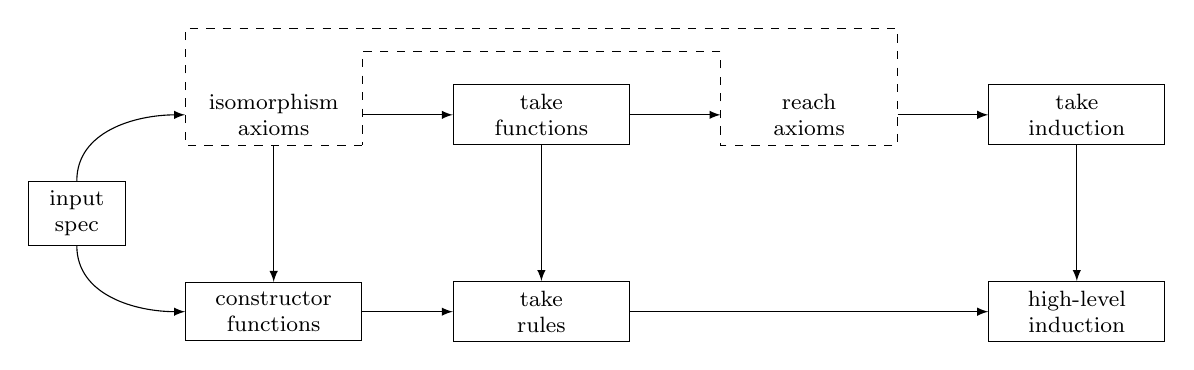
\begin{tikzpicture}
  [ axiom/.style={rectangle, text width=2cm, text centered, font=\footnotesize}
  , proof/.style={rectangle, text width=2cm, text centered, font=\footnotesize, draw}
  , >=latex]
  \node (0) at (-2.5, 1.25) [rectangle, text width=1cm, text centered, font=\footnotesize, draw] {input\\spec};
  \node (1) at (0.0, 2.5) [axiom] {isomorphism\\axioms};
  \node (2) at (3.4, 2.5) [proof] {take\\functions};
  \node (3) at (6.8, 2.5) [axiom] {reach\\axioms};
  \node (4) at (10.2, 2.5) [proof] {take\\induction};
  \node (5) at (0.0, 0.0) [proof] {constructor\\functions};
  \node (6) at (3.4, 0.0) [proof] {take\\rules};
  \node (7) at (10.2, 0.0) [proof] {high-level\\induction};
  \draw [->] (0.north) to [out=90, in=180] (1.west);
  \draw [->] (1) -- (2);
  \draw [->] (2) -- (3);
  \draw [->] (3) -- (4);
  \draw [->] (0.south) to [out=270, in=180] (5.west);
  \draw [->] (1) -- (5);
  \draw [->] (5) -- (6);
  \draw [->] (2) -- (6);
  \draw [->] (6) -- (7);
  \draw [->] (4) -- (7);
  \draw [dashed]
    (1.south east) -- (1.south west) -- (1.north west) --
    (1.west |- 0,3.6) -- (3.east |- 0,3.6) -- (3.south east) -- (3.south west) --
    (3.west |- 0,3.3) -- (1.east |- 0,3.3) -- (1.south east) -- cycle;
%    (1.west |- 0,3.6) -- (4.east |- 0,3.6) -- (4.east |- 0,3.3) --
%    (3.east |- 0,3.3) -- (3.south east) -- (3.south west) --
%    (3.west |- 0,3.3) -- (1.east |- 0,3.3) -- (1.south east) -- cycle;
\end{tikzpicture}
\end{singlespace}
\end{center}
\caption{Domain package implementation schematic}
\label{fig:domain-implementation}
\end{figure}

Another benefit of the new modularization is the ability to swap out individual components. In particular, note that all code involved with generating axioms is contained within the pair of modules inside the dashed lines in Fig.~\ref{fig:domain-implementation}. With clear interfaces between these axiomatic modules and the rest of the \textsc{Domain} package, it will be possible to replace them with definitional versions at a later time, with minimal modifications to the rest of the system. We will come back to the definitional version of the \textsc{Domain} package in Chapter~\ref{ch:universal}.

Each module in Fig.~\ref{fig:domain-implementation} will be explained in more detail in one of the following sections. For each module, we will describe the definitions and proofs that are generated, as well as the ML record types that make up the interfaces.

\subsection{Input specification module}

%%%%%%%%%%%%%%%%%%%%%%%%%%%%%%%%%%%%%%%%%%%%%%%%%%

\begin{figure}
\begin{center}
\begin{minipage}{0.725\linewidth}

\emph{definition}:

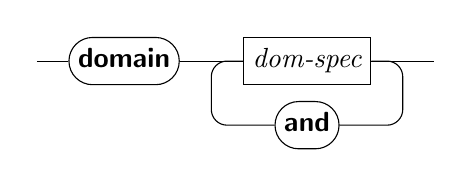
\begin{tikzpicture}
[ thin, draw, text height=1.5ex, text depth=0.4ex
, point/.style={coordinate}
, keyword/.style={rectangle, minimum size=6mm, rounded corners=3mm, draw, font=\bfseries\sffamily}
, terminal/.style={rectangle, minimum size=6mm, rounded corners=3mm, draw, font=\sffamily}
, nonterminal/.style={rectangle, minimum size=6mm, draw, font=\itshape}
, curve/.style={rounded corners=2mm}
]
\matrix[row sep=2mm, column sep=4mm] {
% First row:
\node (p0) [point] {}; &
\node (domain) [keyword] {domain}; &
\node (p3) [point] {}; &
\node (domspec) [nonterminal] {dom-spec}; &
\node (p4) [point] {}; &
\node (p5) [point] {}; \\
% Second row:
& & &
\node (and) [keyword] {and}; \\
};
\draw [curve] (p0) -- (domain) -- (domspec) -- (p5);
\draw [curve] (domspec) -- (p4) |- (and) -| (p3) -- (domspec);
\end{tikzpicture}

%%%%%%%%%%%%%%%%%%%%%%%%%%%%%%%%%%%%%%%%%%%%%%%%%%

\emph{dom-spec}:

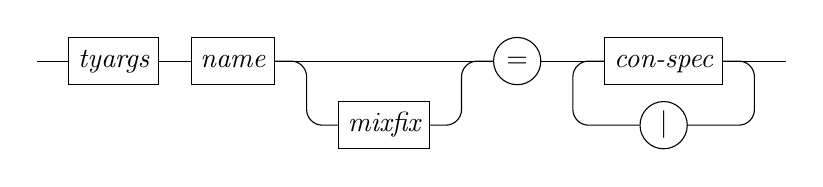
\begin{tikzpicture}
[ thin, draw, text height=1.5ex, text depth=0.4ex
, point/.style={coordinate}
, keyword/.style={rectangle, minimum size=6mm, rounded corners=3mm, draw, font=\bfseries\sffamily}
, terminal/.style={rectangle, minimum size=6mm, rounded corners=3mm, draw, font=\sffamily}
, nonterminal/.style={rectangle, minimum size=6mm, draw, font=\itshape}
, curve/.style={rounded corners=2mm}
]
\matrix[row sep=2mm, column sep=4mm] { 
% First row:
\node (p0) [point] {}; &
\node (tyargs) [nonterminal] {tyargs}; &
\node (name) [nonterminal] {name}; & 
\node (p3) [point] {}; & &
\node (p4) [point] {}; &
\node (equal) [terminal] {=}; &
\node (p5) [point] {}; &
\node (conspec) [nonterminal] {con-spec}; &
\node (p6) [point] {}; &
\node (p7) [point] {}; \\
% Second row:
& & & &
\node (mixfix) [nonterminal] {mixfix}; & & & &
\node (bar) [terminal] {\textbar}; \\
};
\draw [curve] (p0) -- (tyargs) -- (name) -- (equal) -- (conspec) -- (p7);
\draw [curve] (name) -- (p3) |- (mixfix) -| (p4) -- (equal);
\draw [curve] (conspec) -- (p6) |- (bar) -| (p5) -- (conspec);
\end{tikzpicture}

%%%%%%%%%%%%%%%%%%%%%%%%%%%%%%%%%%%%%%%%%%%%%%%%%%

\emph{tyargs}:

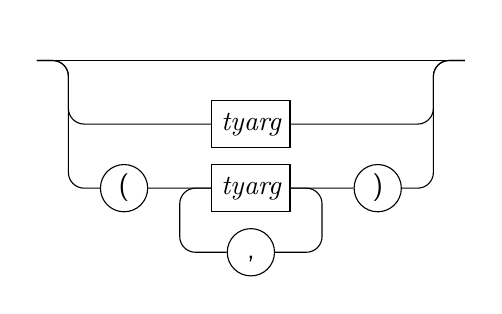
\begin{tikzpicture}
[ thin, draw, text height=1.5ex, text depth=0.4ex
, point/.style={coordinate}
, keyword/.style={rectangle, minimum size=6mm, rounded corners=3mm, draw, font=\bfseries\sffamily}
, terminal/.style={rectangle, minimum size=6mm, rounded corners=3mm, draw, font=\sffamily}
, nonterminal/.style={rectangle, minimum size=6mm, draw, font=\itshape}
, curve/.style={rounded corners=2mm}
]
\matrix[row sep=2mm, column sep=4mm] { 
% First row:
\node (p0) [point] {}; &
\node (p1) [point] {}; & & &
\useasboundingbox circle (3mm); & & &
\node (p2) [point] {}; &
\node (p3) [point] {}; \\
% Second row:
& & & &
\node (tyarg1) [nonterminal] {tyarg}; \\
% Third row:
& &
\node (lparen) [terminal] {(}; &
\node (p8) [point] {}; &
\node (tyarg2) [nonterminal] {tyarg}; &
\node (p9) [point] {}; &
\node (rparen) [terminal] {)}; \\
% Fourth row:
& & & &
\node (comma) [terminal] {,}; \\
};
\draw [curve] (p0) -- (p3);
\draw [curve] (p0) -- (p1) |- (tyarg1) -| (p2) -- (p3);
\draw [curve] (p0) -- (p1) |- (lparen) -- (tyarg2) -- (rparen) -| (p2) -- (p3);
\draw [curve] (tyarg2) -- (p9) |- (comma) -| (p8) -- (tyarg2);
\end{tikzpicture}

%%%%%%%%%%%%%%%%%%%%%%%%%%%%%%%%%%%%%%%%%%%%%%%%%%

\emph{tyarg}:

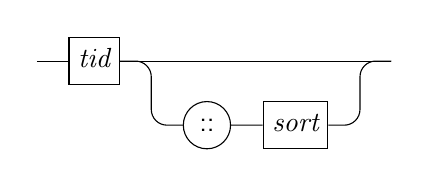
\begin{tikzpicture}
[ thin, draw, text height=1.5ex, text depth=0.4ex
, point/.style={coordinate}
, keyword/.style={rectangle, minimum size=6mm, rounded corners=3mm, draw, font=\bfseries\sffamily}
, terminal/.style={rectangle, minimum size=6mm, rounded corners=3mm, draw, font=\sffamily}
, nonterminal/.style={rectangle, minimum size=6mm, draw, font=\itshape}
, curve/.style={rounded corners=2mm}
]
\matrix[row sep=2mm, column sep=4mm] { 
% First row:
\node (p0) [point] {}; &
\node (tid) [nonterminal] {tid}; &
\node (p1) [point] {}; & & &
\node (p2) [point] {}; &
\node (p3) [point] {}; \\
% Second row:
& & &
\node (colon) [terminal] {::}; &
\node (sort) [nonterminal] {sort}; \\
};
\draw [curve] (p0) -- (tid) -- (p3);
\draw [curve] (tid) -- (p1) |- (colon) -- (sort) -| (p2) -- (p3);
\end{tikzpicture}

%%%%%%%%%%%%%%%%%%%%%%%%%%%%%%%%%%%%%%%%%%%%%%%%%%

\emph{con-spec}:

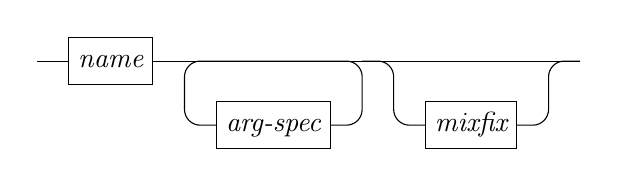
\begin{tikzpicture}
[ thin, draw, text height=1.5ex, text depth=0.4ex
, point/.style={coordinate}
, keyword/.style={rectangle, minimum size=6mm, rounded corners=3mm, draw, font=\bfseries\sffamily}
, terminal/.style={rectangle, minimum size=6mm, rounded corners=3mm, draw, font=\sffamily}
, nonterminal/.style={rectangle, minimum size=6mm, draw, font=\itshape}
, curve/.style={rounded corners=2mm}
]
\matrix[row sep=2mm, column sep=4mm] { 
% First row:
\node (p0) [point] {}; &
\node (name) [nonterminal] {name}; &
\node (p1) [point] {}; & &
\node (p2) [point] {}; &
\node (p3) [point] {}; & &
\node (p4) [point] {}; &
\node (p5) [point] {}; \\
% Second row:
& & &
\node (argspec) [nonterminal] {arg-spec}; & & &
\node (mixfix) [nonterminal] {mixfix}; \\
};
\draw [curve] (p0) -- (name) -- (p5);
\draw [curve] (argspec) -| (p2) -- (p1) |- (argspec);
\draw [curve] (p2) -- (p3) |- (mixfix) -| (p4) -- (p5);
\end{tikzpicture}

%%%%%%%%%%%%%%%%%%%%%%%%%%%%%%%%%%%%%%%%%%%%%%%%%%

\emph{arg-spec}:

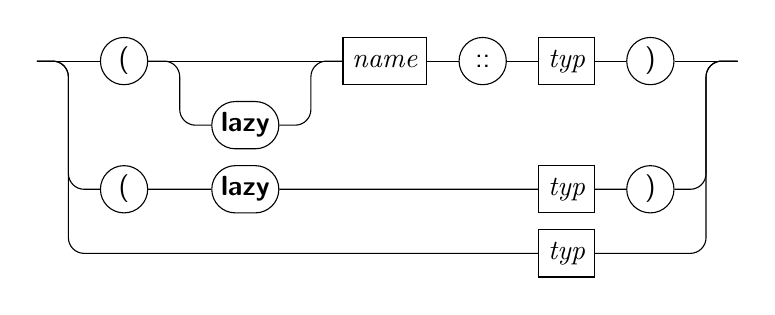
\begin{tikzpicture}
[ thin, draw, text height=1.5ex, text depth=0.4ex
, point/.style={coordinate}
, keyword/.style={rectangle, minimum size=6mm, rounded corners=3mm, draw, font=\bfseries\sffamily}
, terminal/.style={rectangle, minimum size=6mm, rounded corners=3mm, draw, font=\sffamily}
, nonterminal/.style={rectangle, minimum size=6mm, draw, font=\itshape}
, curve/.style={rounded corners=2mm}
]
\matrix[row sep=2mm, column sep=4mm] { 
% First row:
\node (p0) [point] {}; &
\node (p1) [point] {}; &
\node (lparen1) [terminal] {(}; &
\node (p2) [point] {}; & &
\node (p3) [point] {}; &
\node (name) [nonterminal] {name}; &
\node (colon) [terminal] {::}; &
\node (typ1) [nonterminal] {typ}; &
\node (rparen1) [terminal] {)}; &
\node (p4) [point] {}; &
\node (p5) [point] {}; \\
% Second row:
& & & &
\node (lazy1) [keyword] {lazy}; \\
% Third row:
& &
\node (lparen2) [terminal] {(}; & &
\node (lazy2) [keyword] {lazy}; & & & &
\node (typ2) [nonterminal] {typ}; &
\node (rparen2) [terminal] {)}; \\
% Fourth row:
& & & & & & & &
\node (typ3) [nonterminal] {typ}; \\
};
\draw [curve] (p0) -- (lparen1) -- (name) -- (colon) -- (typ1) -- (rparen1) -- (p5);
\draw [curve] (lparen1) -- (p2) |- (lazy1) -| (p3) -- (name);
\draw [curve] (p0) -- (p1) |- (lparen2) -- (lazy2) -- (typ2) -- (rparen2) -| (p4) -- (p5);
\draw [curve] (p0) -- (p1) |- (typ3) -| (p4) -- (p5);
\end{tikzpicture}

\end{minipage}
\end{center}

\caption{Input syntax for {\domain} package}
\label{fig:domain-input-syntax}
\end{figure}

%%%%%%%%%%%%%%%%%%%%%%%%%%%%%%%%%%%%%%%%%%%%%%%%%%

The input-specification module of the \textsc{Domain} package starts by parsing its input according to the grammar shown in Fig.~\ref{fig:domain-input-syntax}. The input consists of one or more domain specifications, each of which has a type on the left-hand side, and a list of constructor specifications on the right. Each constructor has zero or more arguments, either lazy or strict, with an optional selector name for each.

After parsing, the module performs some simple checks, like making sure that there are no duplicate type or constructor names. There are also some more semantic checks: For example, the type of every strict constructor argument must be in class \isa{pcpo}. (Class \isa{cpo} is sufficient for lazy arguments that do not have a selector function.) Another test ensures that recursive occurrences of types are used with the same type arguments. Indirect recursion is also checked for, ensuring that it is only used with acceptable type constructors, including strict sums and products, lifting, and continuous function space. (Recursion under the full function space type constructor is specifically \emph{not} allowed, because it can lead to unsound isomorphism axioms.)

After performing these basic checks on the input, the main task of this module is to prepare information to be passed into the next modules. The input specification module passes information to two others: the isomorphism axioms module and the constructor functions module.

For the isomorphism axioms module, the input specification is transformed into a list of domain equations, one for each new type; information about constructors and selectors is discarded. For example, when defining \isa{domain 'a stream =} \isa{SNil | SCons "'a" (lazy "'a stream")}, the isomorphism module will only see the domain equation \isa{'a stream \<cong> one \<oplus> ('a \<otimes> 'a stream\<^sub>\<bottom>)}. Mutually recursive domain definitions yield multiple domain equations, one for each type. The ML type passed to the isomorphism axioms module is \hs{(binding * mixfix * (typ * typ)) list}, which comprises a type name (ML type \hs{binding}), type constructor syntax (ML type \hs{mixfix}), and the domain equation for each type.

For the constructor functions module, information about the constructors is assembled, using ML type \hs{(binding * (bool * binding option * typ) list *} \hs{mixfix) list}. For each constructor, we have its name, the list of argument specifications, and its syntax; each argument has a boolean laziness flag, an optional selector name, and the argument type. With mutually recursive domain definitions, such a list is assembled for each new type.

\subsection{Isomorphism axioms module}

The input to the isomorphism axioms module consists of a name, syntax, and a domain equation for each new type. The module performs the following steps: First, it \emph{declares} each new type constructor---instead of \emph{defining} them with \textsc{Typedef} or \textsc{Cpodef}, they are simply declared without a definition. Second, a \isa{pcpo} class instance is axiomatically asserted for each type. Third, a pair of \isa{abs} and \isa{rep} functions corresponding to each domain equation is declared---again, without providing a definition. Fourth, isomorphism axioms are generated, asserting that each pair of \isa{abs} and \isa{rep} functions is an isomorphism.

The types, constants, and axioms generated by the isomorphism axioms module are collected in the \hs{iso\_info} record type, shown in Fig.~\ref{fig:domain-iso-info}. The module produces one such record for each mutually recursive domain.

\begin{figure}
\begin{hscode}
type iso_info =
  {
    absT        : typ,    repT        : typ,
    abs_const   : term,   rep_const   : term,
    abs_inverse : thm,    rep_inverse : thm
  }
\end{hscode}
\caption{Record type for domain isomorphisms}
\label{fig:domain-iso-info}
\end{figure}

The supporting theory files for the \textsc{Domain} package define a binary predicate called \isa{iso}, which asserts that its two arguments form a continuous isomorphism.
%
\begin{isacode}
definition iso :: "('a \<rightarrow> 'b) \<Rightarrow> ('b \<rightarrow> 'a) \<Rightarrow> bool"
  where "iso abs rep \<longleftrightarrow> (\<forall>x. rep\<cdot>(abs\<cdot>x) = x) \<and> (\<forall>y. abs\<cdot>(rep\<cdot>y) = y)"
\end{isacode}
%
The axioms declared by the isomorphism module are sufficient to derive \isa{iso abs rep} as a theorem. (An alternative design would be to declare \isa{iso abs rep} directly as the axiom.) Other modules will use the \isa{iso} predicate to derive various other properties of the \isa{abs} and \isa{rep} functions.

\subsection{Take functions module}

The take functions module accepts input of type \hs{(binding * iso\_info) list}, comprising a type name and isomorphism information for each new type. The module defines a take function for each type and generates several theorems about them, which are collected in an ML record of type \hs{take\_info} (Fig.~\ref{fig:domain-take-info}).

\begin{figure}
\begin{hscode}
type take_info =
  {
    take_consts         : term list,   take_defs     : thm list,
    chain_take_thms     : thm list,    take_0_thms   : thm list,
    take_strict_thms    : thm list,    take_Suc_thms : thm list,
    deflation_take_thms : thm list
  }
\end{hscode}
\caption{Record type for take functions and related theorems}
\label{fig:domain-take-info}
\end{figure}
% I omit finite_consts and finite_defs, because they are irrelevant and uninteresting.

\paragraph{Defining the take functions.} Below is the take function for the stream data\-type, which is a solution to \isa{'a stream \<cong> one \<oplus> ('a \<otimes> 'a stream\<^sub>\<bottom>)}. The take function \isa{stream_take n} is defined as the \isa{n}th iteration of a certain functional, consisting of \isa{stream_abs} and \isa{stream_rep} composed with a combination of map functions. The map functions are in a one-to-one correspondence with the type constructors that appear on the right-hand side of the domain equation.
%
\begin{isacode}
definition stream_take :: "nat \<Rightarrow> 'a stream \<rightarrow> 'a stream"
  where "stream_take n \<equiv> iterate n\<cdot>(\<Lambda> f.
    stream_abs oo ssum_map\<cdot>ID\<cdot>(sprod_map\<cdot>ID\<cdot>(u_map\<cdot>f)) oo stream_rep)\<cdot>\<bottom>"
\end{isacode}

To keep track of the map combinators associated with each type constructor, the \textsc{Domain} package maintains a database of theorems with the \isa{[domain_map_ID]} attribute. Using a theorem attribute makes it relatively easy to add support for additional type constructors, by adding new theorems to the database. The theorems making up the initial contents of the database are shown in Fig.~\ref{fig:domain-map-ID}. We can use these rules to generate a combination of map functions corresponding to any given complex type expression: Starting with the identity function \isa{ID} at the given type, perform rewriting with the \isa{domain_map_ID} rules, applying them right-to-left.

\begin{figure}
\indexthm{domain_map_ID}
\begin{isacode}
lemma [domain_map_ID]:
  "u_map\<cdot>(ID :: 'a \<rightarrow> 'a) = (ID :: 'a\<^sub>\<bottom> \<rightarrow> 'a\<^sub>\<bottom>)"
  "prod_map\<cdot>(ID :: 'a \<rightarrow> 'a)\<cdot>(ID :: 'b \<rightarrow> 'b) = (ID :: 'a \<times> 'b \<rightarrow> 'a \<times> 'b)"
  "sprod_map\<cdot>(ID :: 'a \<rightarrow> 'a)\<cdot>(ID :: 'b \<rightarrow> 'b) = (ID :: 'a \<otimes> 'b \<rightarrow> 'a \<otimes> 'b)"
  "ssum_map\<cdot>(ID :: 'a \<rightarrow> 'a)\<cdot>(ID :: 'b \<rightarrow> 'b) = (ID :: 'a \<oplus> 'b \<rightarrow> 'a \<oplus> 'b)"
  "cfun_map\<cdot>(ID :: 'a \<rightarrow> 'a)\<cdot>(ID :: 'b \<rightarrow> 'b) = (ID :: ('a \<rightarrow> 'b) \<rightarrow> ('a \<rightarrow> 'b))"
\end{isacode}
\caption{Extensible set of rules with the \isa{domain_map_ID} attribute}
\label{fig:domain-map-ID}
\end{figure}

For mutually recursive domains, the take functions are defined in a manner similar to how \textsc{Fixrec} handles mutual recursion: We construct a functional that operates on tuples, and then project out the desired component using \isa{fst} and \isa{snd}.

\begin{isacode}
domain 'a list1 = Nil1 | List2 "'a list2" and 'a list2 = Cons2 "'a" "'a list1"
\end{isacode}
\unmedskip
\begin{isacode}
definition list1_take :: "nat \<Rightarrow> 'a list1 \<rightarrow> 'a list1"
  where "list1_take n \<equiv> fst (iterate n\<cdot>
        (\<Lambda> f. (list1_abs oo ssum_map\<cdot>ID\<cdot>(snd f) oo list1_rep,
            list2_abs oo sprod_map\<cdot>ID\<cdot>(fst f) oo list2_rep))\<cdot>\<bottom>)"
\end{isacode}
\unmedskip
\begin{isacode}
definition list2_take :: "nat \<Rightarrow> 'a list2 \<rightarrow> 'a list2"
  where "list2_take n \<equiv> snd (iterate n\<cdot>
        (\<Lambda> f. (list1_abs oo ssum_map\<cdot>ID\<cdot>(snd f) oo list1_rep,
            list2_abs oo sprod_map\<cdot>ID\<cdot>(fst f) oo list2_rep))\<cdot>\<bottom>)"
\end{isacode}

Note that unlike mutual recursion, indirect recursion does not require any special treatment. Of the following two variations of the \isa{bintree} datatype, one is indirect-recursive and the other is not. However, they both give rise to the same domain equation, and so the take function is defined identically for either one.

\begin{isacode}
domain bintree = Tip | Branch "bintree \<otimes> bintree"
\end{isacode}
\unmedskip
\begin{isacode}
domain bintree = Tip | Branch "bintree" "bintree"
\end{isacode}
\unmedskip

\paragraph{Proving theorems about take functions.} After defining the take functions, the take function module proves several theorems about them. We will consider the stream datatype as an example.
%
\indexthmx{stream.chain_take}
\begin{isacode}
theorem stream.chain_take [simp]: "chain (\<lambda>n. stream_take n)"
\end{isacode}
\unmedskip
\indexthmx{stream.take_0}
\begin{isacode}
theorem stream.take_0 [simp]: "stream_take 0 = \<bottom>"
\end{isacode}
\unmedskip
\indexthmx{stream.take_Suc}
\begin{isacode}
theorem stream.take_Suc: "stream_take (Suc n) = stream_abs oo
  ssum_map\<cdot>ID\<cdot>(sprod_map\<cdot>ID\<cdot>(u_map\<cdot>(stream_take n))) oo stream_rep"
\end{isacode}
%
These first few lemmas are easy to prove. Theorem \isa{stream.chain_take} follows from the fact that \isa{(\<lambda>n. iterate n\<cdot>F\<cdot>\<bottom>)} is always a chain. (For mutually recursive take functions, note that \isa{fst} and \isa{snd} are monotone, and thus preserve chains.) The \isa{take_0} and \isa{take_Suc} theorems follow directly from the definitions by the properties of \isa{iterate}.

To help derive the other properties of \isa{stream_take}, we make use of a new concept: A \emph{deflation} is a continuous function \isa{f} that is idempotent and below the identity function, so that \isa{f oo f = f \<sqsubseteq> ID}. These are properties that are expected to hold for every take function. We define the \isa{deflation} predicate as follows.\footnote{The \isa{deflation} predicate is actually defined with a \isa{locale} command, which generates a definition equivalent to the one shown here.}

\begin{isacode}
definition deflation :: "('a \<rightarrow> 'a) \<Rightarrow> bool"
  where "deflation d \<longleftrightarrow> (\<forall>x. d\<cdot>(d\<cdot>x) = d\<cdot>x) \<and> (\<forall>x. d\<cdot>x \<sqsubseteq> x)"
\end{isacode}

Showing that each take function is a deflation is the only really non-trivial proof done by the take functions module. Once it is proved that \isa{stream_take} is a chain of deflations, the module can easily derive the rest of the desired theorems about \isa{stream_take}.
%
\indexthmx{stream.deflation_take}
\begin{isacode}
theorem stream.deflation_take: "deflation (stream_take n)"
\end{isacode}
%
The proof of \isa{stream.deflation_take} proceeds by induction on \isa{n}. After unfolding \isa{stream.take_0}, the base case is trivial, because \isa{\<bottom>} is a deflation. In the inductive case, we start by unfolding \isa{stream.take_Suc}. A suitably-instantiated rule \isa{deflation_abs_rep} is applied next, followed by deflation lemmas for the various map combinators. The \textsc{Domain} package maintains a database of deflation lemmas that have the \isa{[domain_deflation]} attribute; Fig.~\ref{fig:domain-deflation} shows the initial set of \isa{domain_deflation} rules.
%
\indexthm{deflation_abs_rep}
\begin{isacode}
lemma deflation_abs_rep:
  "\<lbrakk>iso abs rep; deflation d\<rbrakk> \<Longrightarrow> deflation (abs oo d oo rep)"
\end{isacode}
%
For mutually recursive domains, the \isa{deflation_take} rules for all take functions must be proved simultaneously, with a single induction on \isa{n}. The other steps in the deflation proof are similar to the single-domain case.

\begin{figure}
\indexthm{domain_map_ID}
\begin{isacode}
lemma [domain_deflation]:
  "deflation ID"
  "deflation f \<Longrightarrow> deflation (u_map\<cdot>f)"
  "\<lbrakk>deflation f; deflation g\<rbrakk> \<Longrightarrow> deflation (prod_map\<cdot>f\<cdot>g)"
  "\<lbrakk>deflation f; deflation g\<rbrakk> \<Longrightarrow> deflation (sprod_map\<cdot>f\<cdot>g)"
  "\<lbrakk>deflation f; deflation g\<rbrakk> \<Longrightarrow> deflation (ssum_map\<cdot>f\<cdot>g)"
  "\<lbrakk>deflation f; deflation g\<rbrakk> \<Longrightarrow> deflation (cfun_map\<cdot>f\<cdot>g)"
\end{isacode}
\caption{Extensible set of rules with the \isa{domain_deflation} attribute}
\label{fig:domain-deflation}
\end{figure}

After proving \isa{stream.deflation_take}, we can derive the other theorems. Rules \isa{stream.take_below} and \isa{stream.take_strict} follow directly from \isa{stream.deflation_take}. Theorem \isa{stream.take_take} also depends on the fact that \isa{stream_take} is a chain, using the library lemma \isa{deflation_chain_min}.

\indexthmx{stream.take_below}
\begin{isacode}
theorem stream.take_below: "stream_take n\<cdot>x \<sqsubseteq> x"
\end{isacode}
\unmedskip
\indexthmx{stream.take_strict}
\begin{isacode}
theorem stream.take_strict: "stream_take n\<cdot>\<bottom> = \<bottom>"
\end{isacode}
\unmedskip
\indexthmx{stream.take_take}
\begin{isacode}
theorem stream.take_take:
  "stream_take m\<cdot>(stream_take n\<cdot>x) = stream_take (min m n)\<cdot>x"
\end{isacode}
\unmedskip
\indexthm{deflation_chain_min}
\begin{isacode}
lemma deflation_chain_min:
  "\<lbrakk>chain t; \<And>n. deflation (t n)\<rbrakk> \<Longrightarrow> t m\<cdot>(t n\<cdot>x) = t (min m n)\<cdot>x"
\end{isacode}
%
Finally, the take functions module collects the relevant theorems in a \hs{take\_info} record, to be passed along to the later modules.

\subsection{Reach axioms module}

For each take function, the {\domain} package declares an axiom stating that the least upper bound of the chain of take functions is the identity function. For example, with the \isa{'a stream} type, the following axiom is declared:
%
\begin{isacode}
axioms stream.lub_take: "(\<Squnion>n. stream_take n) = ID"
\end{isacode}
%
For mutually recursive domain definitions, one axiom is declared for each new type. This list of axioms is then passed along to the take induction module.

\subsection{Take induction module}

The take induction module takes three pieces of input: a list of type \hs{(binding *} \hs{iso\_info) list} from the isomorphism axioms module, a \hs{take\_info} record from the take functions module, and a \hs{thm list} containing \isa{lub_take} theorems from the reach axioms module. The take induction module then derives a few low-level induction principles involving the take functions, and packages up the results in an ML record of type \hs{take\_induct\_info} (Fig.~\ref{fig:domain-take-induct-info}).

\begin{figure}
\begin{hscode}
type take_induct_info =
  {
    take_info         : take_info,
    lub_take_thms     : thm list,
    reach_thms        : thm list,
    take_lemma_thms   : thm list,
    is_finite         : bool,
    take_induct_thms  : thm list
  }
\end{hscode}
\caption{Record type for \textsc{Domain} package theorems related to take induction}
\label{fig:domain-take-induct-info}
\end{figure}

For each new type, the take induction module generates three new theorems in addition to the \isa{lub_take} axiom: the reach lemma, the take lemma, and the take induction rule. For the stream datatype, these are as follows.
%
\indexthmx{stream.reach}
\begin{isacode}
theorem stream.reach: "(\<Squnion>n. stream_take n\<cdot>x) = x"
\end{isacode}
\unmedskip
\indexthmx{stream.take_lemma}
\begin{isacode}
theorem stream.take_lemma:
  "(\<And>n. stream_take n\<cdot>x = stream_take n\<cdot>y) \<Longrightarrow> x = y"
\end{isacode}
\unmedskip
\indexthmx{stream.take_induct}
\begin{isacode}
theorem stream.take_induct: "\<lbrakk>adm P; \<And>n. P (stream_take n\<cdot>x)\<rbrakk> \<Longrightarrow> P x"
\end{isacode}
%
Each of these is derived easily from theorems \isa{stream.chain_take} and \isa{stream.lub_take}, using an appropriate library lemma.
%
\indexthm{lub_ID_reach}
\begin{isacode}
lemma lub_ID_reach:
  assumes "chain t" and "(\<Squnion>n. t n) = ID"
  shows "(\<Squnion>n. t n\<cdot>x) = x"
\end{isacode}
\unmedskip
\indexthm{lub_ID_take_lemma}
\begin{isacode}
lemma lub_ID_take_lemma:
  assumes "chain t" and "(\<Squnion>n. t n) = ID"
  shows "(\<And>n. t n\<cdot>x = t n\<cdot>y) \<Longrightarrow> x = y"
\end{isacode}
\unmedskip
\indexthmx{lub_ID_take_induct}
\begin{isacode}
lemma lub_ID_take_induct:
  assumes "chain t" and "(\<Squnion>n. t n) = ID"
  shows "\<lbrakk>adm P; \<And>n. P (t n\<cdot>x)\<rbrakk> \<Longrightarrow> P x"
\end{isacode}

\paragraph{Finite-valued domains.}  The take induction module's job is not always quite this easy. Recall that strict recursive datatypes contain only finite values: In these cases we must generate a take induction rule without an admissibility condition.

To determine whether or not a domain (or set of mutually recursive domains) is finite-valued, the take induction module performs a test on its associated domain equation. For example, consider the strict list datatype:
%
\begin{isacode}
domain 'a strictlist = nil | cons "'a" "'a strictlist"
\end{isacode}
%
The domain equation is \isa{'a strictlist \<cong> one \<oplus> ('a \<otimes> 'a strictlist)}. Note that the only type constructors surrounding the recursive occurrence of \isa{'a strictlist} on the right-hand side are the strict sum and strict product. This indicates that \isa{'a strictlist} is a finite-valued domain. Equivalently, we might notice that the only map combinators mentioned in the definition of \isa{strictlist_take} are \isa{ssum_map} and \isa{sprod_map}.
%
\indexdefx{strictlist.take_Suc}
\begin{isacode}
theorem strictlist.take_Suc: "strictlist_take (Suc n) = strictlist_abs oo
  ssum_map\<cdot>ID\<cdot>(sprod_map\<cdot>ID\<cdot>(strictlist_take n)) oo strictlist_rep"
\end{isacode}
%
On the other hand, for lazy streams we have \isa{'a stream \<cong> one \<oplus> ('a \<otimes> 'a stream\<^sub>\<bottom>)} as the domain equation. The presence of lifting on the recursive occurrence of \isa{'a stream} indicates that this is \emph{not} a finite-valued domain.

In order to prove a take induction principle for \isa{'a strictlist} without an admissibility condition, we will show that \isa{strictlist_take} satisfies a particular property, which we call \emph{decisiveness}. (Note that decisiveness is not a standard concept in domain theory, but rather an invention of the present author.) A decisive function is a particular kind of deflation that makes an all-or-nothing choice for each input value: The function either returns its input value, or else it returns \isa{\<bottom>}. The HOLCF definition of the predicate \isa{decisive} is shown in Fig.~\ref{fig:domain-decisive}, along with several related lemmas. Note that decisiveness is preserved by \isa{ssum_map} and \isa{sprod_map}, but not by any of the other map combinators; this is why it is important that only \isa{ssum_map} and \isa{sprod_map} are used in the definition of \isa{strictlist_take}. 

\begin{figure}
\indexdef{decisive}
\begin{isacode}
definition decisive :: "('a \<rightarrow> 'a) \<Rightarrow> bool"
  where "decisive f \<longleftrightarrow> (\<forall>x. f\<cdot>x = x \<or> f\<cdot>x = \<bottom>)"
\end{isacode}
\unmedskip
\indexthm{decisive_bottom}
\begin{isacode}
lemma decisive_bottom: "decisive \<bottom>"
\end{isacode}
\unmedskip
\indexthm{decisive_ID}
\begin{isacode}
lemma decisive_ID: "decisive ID"
\end{isacode}
\unmedskip
\indexthm{decisive_ssum_map}
\begin{isacode}
lemma decisive_ssum_map: "\<lbrakk>decisive f; decisive g\<rbrakk> \<Longrightarrow> decisive (ssum_map\<cdot>f\<cdot>g)"
\end{isacode}
\unmedskip
\indexthm{decisive_sprod_map}
\begin{isacode}
lemma decisive_sprod_map: "\<lbrakk>decisive f; decisive g\<rbrakk> \<Longrightarrow> decisive (sprod_map\<cdot>f\<cdot>g)"
\end{isacode}
\unmedskip
\indexthm{decisive_abs_rep}
\begin{isacode}
lemma decisive_abs_rep: "\<lbrakk>iso abs rep; decisive f\<rbrakk> \<Longrightarrow> decisive (abs oo f oo rep)"
\end{isacode}
\caption{Definition and properties of decisive deflations}
\label{fig:domain-decisive}
\end{figure}

The proof of \isa{decisive (strictlist_take n)} proceeds by induction on \isa{n}. Each case is solved with the help of the various lemmas about \isa{decisive} shown in Fig.~\ref{fig:domain-decisive}. The proof structure is exactly the same as for the \isa{deflation_take} proofs done by the take functions module.

Having proved the decisiveness of \isa{strictlist_take}, the take induction rule can be derived using the library lemma \isa{lub_ID_finite_take_induct}.
%
\begin{isacode}
lemma lub_ID_finite_take_induct:
  assumes "chain t" and "(\<Squnion>n. t n) = ID" and "\<And>n. decisive (t n)"
  shows "(\<And>n. P (t n\<cdot>x)) \<Longrightarrow> P x"
\end{isacode}
%
To prove this lemma, it is sufficient to show that there exists \isa{n} such that \isa{t n\<cdot>x = x}. Now consider the chain \isa{(\<lambda>n. t n\<cdot>x)}, which has a finite range: Because each \isa{t n} is decisive, the chain's range is a subset of \isa{\<lbrace>\<bottom>, x\<rbrace>}. As a finite chain, it must attain its least upper bound at some point.

Ultimately the take induction module wraps up all the new theorems in a \hs{take\_induct\_info} record to pass along to the induction rules module. This record also includes the original \hs{take\_info} record, and a boolean flag to indicate finite-valued domains.

\subsection{Constructor functions module}

The constructor functions module is called with three pieces of input: a \hs{binding} for the type name, an \hs{iso\_info} record from the isomorphism axioms module, and a list of constructor specifications of type \hs{(binding * (bool * binding option *} \hs{typ) list * mixfix) list}. Each call to the module deals with a single domain equation; with mutually recursive definitions the module is called multiple times, once for each new type.

%The constructor functions module returns a record of type \hs{constr\_info} that is filled with generated constants and theorems (Fig.~\ref{fig:domain-constr-info}). The remainder of this section is organized into subheadings, each corresponding to one or more fields of this record.
The constructor functions module returns a \hs{constr\_info} record filled with generated constants and theorems (Fig.~\ref{fig:domain-constr-info}). The remainder of this section is organized into subheadings, each corresponding to one or more fields of this record.

\begin{figure}
\begin{hscode}
type constr_info =
  {
    iso_info  : iso_info,
    con_specs : (term * (bool * typ) list) list,
    con_betas : thm list,
    nchotomy  : thm,         exhaust    : thm,
    compacts  : thm list,    con_rews   : thm list,
    inverts   : thm list,    injects    : thm list,
    dist_les  : thm list,    dist_eqs   : thm list,
    case_rews : thm list,    sel_rews   : thm list,
    dis_rews  : thm list,    match_rews : thm list
  }
\end{hscode}
\caption{Record type for constructor-related constants and theorems}
\label{fig:domain-constr-info}
\end{figure}

The \isa{'a stream} type is a bit too simple to adequately demonstrate all the features of the constructor functions module. Instead, we will use this slightly more complex \isa{('a, 'b) tree} datatype as a running example.

\begin{isacode}
domain ('a, 'b) tree =
  Tip | Leaf "'a" |
  Node (left :: "('a, 'b) tree") (lazy middle :: "'b") (right :: "('a, 'b) tree")
\end{isacode}

\paragraph{Defining the constructors.} Each constructor is defined using the \isa{tree_abs} function from the isomorphism together with some combination of the HOLCF data constructors \isa{spair}, \isa{sinl}, \isa{sinr}, \isa{ONE}, and \isa{up}.
%
\begin{isacode}
  "Tip = abs_tree`(sinl`ONE)"
  "Leaf = (\<Lambda> a. abs_tree`(sinr`(sinl`a)))"
  "Node = (\<Lambda> t1 b t2. abs_tree`(sinr`(sinr`(:t1, up`b, t2:))))"
\end{isacode}
%
At the time the constructor constants are defined, the module also declares any infix syntax that may have been specified.

After defining the constructor functions, the module fills in the \hs{con\_specs} field of result record with an ML value of type \hs{(term * (bool * typ) list) list}. For each constructor, we have the actual constructor constant (ML type \hs{term}) and a list of argument specifications, each consisting of a laziness flag and an argument type. We discard information about syntax and selector functions, because the induction rules module does not need it.

After defining the constructor functions, the next step is to prove rules for unfolding the definitions of fully-applied constructors. These rules occupy the \hs{con\_betas} field of the results record, and will be used in many other internal proofs.

Each constructor function is defined with continuous lambda abstractions, which require continuity checks to beta-reduce. Domain definitions with many-argument constructors produce equally large numbers of continuity conditions, which can get expensive to check. For this reason, we use the bottom-up continuity proof method described in Chapter~\ref{ch:holcf}, which saves time by reusing common subproofs.

\begin{isacode}
have con_betas:
  "Tip = abs_tree`(sinl`ONE)"
  "\<And>a. Leaf`a = abs_tree`(sinr`(sinl`a))"
  "\<And> t1 b t2. Node`t1`b`t2 = abs_tree`(sinr`(sinr`(:t1, up`b, t2:)))"
\end{isacode}

The original \HOLCF{99} \textsc{Domain} package did not have an equivalent of the \isa{con_betas} rules. Instead, every proof about the constructors simply unfolded the raw constructor definitions, and beta-reduced them using the simplifier. Thus the same continuity checks were done again and again, separately in each generated theorem---and even worse, the time required for each check was exponential in the number of nested lambdas. For domain definitions with constructors of more than two or three arguments, the continuity proofs dominated the entire running time of the \textsc{Domain} package, and constructors with more than four or five arguments were simply infeasible. In contrast, the \HOLCF{11} \textsc{Domain} package scales much better to large numbers of constructor arguments; continuity checks are no longer a performance bottleneck.

\paragraph{Exhaustiveness of constructors.}

After defining the constructors, the \textsc{Domain} package proceeds to prove that the constructors are exhaustive. The \HOLCF{11} \textsc{Domain} package uses a novel proof method, based on rewriting, to generate the exhaustiveness theorem efficiently; we will examine it in some detail.

The method involves generating a type-specific exhaustiveness rule starting from a generic one, using a set of type-directed rewrite rules. The generic starting rule, which is valid for any \isa{pcpo}, is called \isa{exh_start}; it merely states that any value \isa{p} either is or is not equal to \isa{\<bottom>}.
%
\indexthm{exh_start}
\begin{isacode}
lemma exh_start: "p = \<bottom> \<or> (\<exists>x. p = x \<and> x \<noteq> \<bottom>)"
\end{isacode}
%
Next, we have the set of type-directed rewrite rules:
%
\begin{isacode}
lemma ex_bottom_iffs:
  "(\<exists>x. P x \<and> x \<noteq> \<bottom>) \<longleftrightarrow> (\<exists>x. P (sinl\<cdot>x) \<and> x \<noteq> \<bottom>) \<or> (\<exists>x. P (sinr\<cdot>x) \<and> x \<noteq> \<bottom>)"
  "(\<exists>x. P x \<and> x \<noteq> \<bottom>) \<longleftrightarrow> (\<exists>x y. (P (:x, y:) \<and> x \<noteq> \<bottom>) \<and> y \<noteq> \<bottom>)"
  "(\<exists>x. P x \<and> x \<noteq> \<bottom>) \<longleftrightarrow> (\<exists>x y. P (:up\<cdot>x, y:) \<and> y \<noteq> \<bottom>)"
  "(\<exists>x. P x \<and> x \<noteq> \<bottom>) \<longleftrightarrow> (\<exists>x. P (up\<cdot>x))"
  "(\<exists>x. P x \<and> x \<noteq> \<bottom>) \<longleftrightarrow> P ONE"
\end{isacode}
%
Each of the rewrite rules has the same pattern on the left-hand side, namely \isa{(\<exists>x. P x \<and> x \<noteq> \<bottom>)}. However, each of these rules places a different type constraint on the variable \isa{x}. Also note that many of the rules' right-hand sides also contain instances of the same pattern, but at smaller types. So rewriting with \isa{ex_bottom_iffs} may continue for several steps, but it always terminates.

Now we will step through the process of deriving an exhaustiveness theorem for the \isa{('a, 'b) tree} datatype. We start by instantiating the theorem \isa{exh_start} at a type similar to the representation type for \isa{('a, 'b) tree}.
%
\begin{isacode}
have thm1: "(p :: one \<oplus> 'a \<oplus> ('c \<otimes> 'b\<^sub>\<bottom> \<otimes> 'd)) = \<bottom> \<or> (\<exists>x. p = x \<and> x \<noteq> \<bottom>)"
\end{isacode}
%
Next, we rewrite this intermediate theorem, using the rules in \isa{ex_bottom_iffs}.
%
\begin{isacode}
have thm2: "p = \<bottom> \<or> p = sinl\<cdot>ONE \<or> (\<exists>x. p = sinr\<cdot>(sinl\<cdot>x) \<and> x \<noteq> \<bottom>) \<or>
  (\<exists>x y z. (p = sinr\<cdot>(sinr\<cdot>(:x, up\<cdot>y, z:)) \<and> x \<noteq> \<bottom>) \<and> z \<noteq> \<bottom>)"
\end{isacode}
%
Then \isa{thm2} is rewritten to re-associate the conjunctions to the right, resulting in another temporary theorem \isa{thm3}. Now we will use \isa{thm3} to prove that the constructors of domain \isa{('a, 'b) tree} are exhaustive:
%
\indexthmx{tree.nchotomy}
\begin{isacode}
theorem tree.nchotomy:
  "y = \<bottom> \<or> y = Tip \<or> (\<exists>a. y = Leaf\<cdot>a \<and> a \<noteq> \<bottom>) \<or>
    (\<exists>t1 b t2. y = Node\<cdot>t1\<cdot>b\<cdot>t2 \<and> t1 \<noteq> \<bottom> \<and> t2 \<noteq> \<bottom>)"
\end{isacode}
%
The proof starts by unfolding \isa{con_betas}. Next, we can rewrite occurrences of \isa{x = tree_abs\<cdot>y} to \isa{tree_rep\<cdot>x = y}, and \isa{x = \<bottom>} to \isa{tree_rep\<cdot>x = \<bottom>}, using rules derived from the isomorphism axioms. This produces a goal that can be solved directly by the temporary theorem \isa{thm3}.

After proving \isa{tree.nchotomy}, the case analysis rule \isa{tree.exhaust} can be derived from it.
%
\indexthmx{tree.exhaust}
\begin{isacode}
theorem tree.exhaust:
  "\<lbrakk>y = \<bottom> \<Longrightarrow> P; y = Tip \<Longrightarrow> P; \<And>a. \<lbrakk>y = Leaf\<cdot>a; a \<noteq> \<bottom>\<rbrakk> \<Longrightarrow> P;
    \<And>t1 b t2. \<lbrakk>y = Node\<cdot>t1\<cdot>b\<cdot>t2; t1 \<noteq> \<bottom>; t2 \<noteq> \<bottom>\<rbrakk> \<Longrightarrow> P\<rbrakk> \<Longrightarrow> P"
\end{isacode}
%
The derivation starts by composing \isa{tree.nchotomy} with \isa{exh_casedist0}; this rule transforms a theorem with conclusion \isa{R} into an elimination rule of the form \isa{(R \<Longrightarrow> P) \<Longrightarrow> P}. This rule is then rewritten with \isa{exh_casedists}, yielding theorem \isa{tree.exhaust}.
%
\indexthm{exh_casedist0}
\begin{isacode}
lemma exh_casedist0: "\<lbrakk>R; R \<Longrightarrow> P\<rbrakk> \<Longrightarrow> P"
\end{isacode}
\unmedskip
\indexthm{exh_casedists}
\begin{isacode}
lemma exh_casedists:
  "((P \<or> Q \<Longrightarrow> R) \<Longrightarrow> S) \<equiv> (\<lbrakk>P \<Longrightarrow> R; Q \<Longrightarrow> R\<rbrakk> \<Longrightarrow> S)"
  "((\<exists>x. P x) \<Longrightarrow> Q) \<equiv> (\<And>x. P x \<Longrightarrow> Q)"
  "(P \<and> Q \<Longrightarrow> R) \<equiv> (\<lbrakk>P; Q\<rbrakk> \<Longrightarrow> R)"
\end{isacode}

These proof methods for generating \isa{nchotomy} and \isa{exhaust} theorems are far faster than the methods used by the \HOLCF{99} \textsc{Domain} package. In the earlier version, these theorems were proved by repeatedly performing case analyses on strict sum and product types. Many redundant cases involving \isa{\<bottom>} were produced, each of which had to be solved by the simplifier. The number of such steps was proportional to the size of the definition; the time spent on this one proof made up a significant portion of the running time for the \textsc{Domain} package. In contrast, the new version calls a short, finite list of proof tactics that all run quickly.

\paragraph{Simplification rules for constructors.}

The constructor functions module generates several groups of simplification rules about the constructors: There are rules about compactness, strictness, definedness, distinctness, injectivity, and order comparisons.

\begin{itemize*}
\item \isa{tree.compacts}: For each constructor, we get a rule stating that the constructor is compact if all its arguments are compact.
%
\begin{isacode}
"compact Tip"
"compact a \<Longrightarrow> compact (Leaf\<cdot>a)"
"\<lbrakk>compact t1; compact b; compact t2\<rbrakk> \<Longrightarrow> compact (Node\<cdot>t1\<cdot>b\<cdot>t2)"
\end{isacode}

\item \isa{tree.con_rews} (1): For each non-lazy argument position of each constructor, we get a strictness rule showing that the constructor applied to \isa{\<bottom>} equals \isa{\<bottom>}.
%
\begin{isacode}
"Leaf\<cdot>\<bottom> = \<bottom>"
"Node\<cdot>\<bottom>\<cdot>b\<cdot>t2 = \<bottom>"
"Node\<cdot>t1\<cdot>b\<cdot>\<bottom> = \<bottom>"
\end{isacode}

\item \isa{tree.con_rews} (2): For each constructor, we get a definedness rule stating that the constructor equals \isa{\<bottom>} if and only if one of its non-lazy arguments equals \isa{\<bottom>}. The proofs are by unfolding \isa{con_betas} and simplifying with definedness rules for \isa{tree_abs}, \isa{sinl}, \isa{sinr}, \isa{spair}, \isa{up}, and \isa{ONE}.
%
\begin{isacode}
"Tip \<noteq> \<bottom>"
"Leaf\<cdot>a = \<bottom> \<longleftrightarrow> a = \<bottom>"
"Node\<cdot>t1\<cdot>b\<cdot>t2 = \<bottom> \<longleftrightarrow> t1 = \<bottom> \<or> t2 = \<bottom>"
\end{isacode}

\item \isa{tree.dist_les}: For each pair of distinct constructors, we get a rule stating that constructor 1 is below constructor 2 if and only if one of the non-lazy arguments of constructor 1 is \isa{\<bottom>}.
%
\begin{isacode}
"Tip \<notsqsubseteq> Leaf\<cdot>a'"
"Tip \<notsqsubseteq> Node\<cdot>t1'\<cdot>b'\<cdot>t2'"
"Leaf\<cdot>a \<sqsubseteq> Tip \<longleftrightarrow> a = \<bottom>"
"Leaf\<cdot>a \<sqsubseteq> Node\<cdot>t1'\<cdot>b'\<cdot>t2' \<longleftrightarrow> a = \<bottom>"
"Node\<cdot>t1\<cdot>b\<cdot>t2 \<sqsubseteq> Tip \<longleftrightarrow> t1 = \<bottom> \<or> t2 = \<bottom>"
"Node\<cdot>t1\<cdot>b\<cdot>t2 \<sqsubseteq> Leaf\<cdot>a' \<longleftrightarrow> t1 = \<bottom> \<or> t2 = \<bottom>"
\end{isacode}

\item \isa{tree.dist_eqs}: For each pair of distinct constructors, we get a rule stating that constructor 1 is equal to constructor 2 if and only if both constructors have at least one non-lazy argument equal to \isa{\<bottom>}.
%
\begin{isacode}
"Tip \<noteq> Leaf\<cdot>a'"
"Tip \<noteq> Node\<cdot>t1'\<cdot>b'\<cdot>t2'"
"Leaf\<cdot>a \<noteq> Tip"
"Leaf\<cdot>a = Node\<cdot>t1'\<cdot>b'\<cdot>t2' \<longleftrightarrow> a = \<bottom> \<and> (t1' = \<bottom> \<or> t2' = \<bottom>)"
"Node\<cdot>t1\<cdot>b\<cdot>t2 \<noteq> Tip"
"Node\<cdot>t1\<cdot>b\<cdot>t2 = Leaf\<cdot>a' \<longleftrightarrow> (t1 = \<bottom> \<or> t2 = \<bottom>) \<and> a' = \<bottom>"
\end{isacode}

\item \isa{tree.inverts}: For each constructor (except those with no arguments) we have a rule stating that two applications of the same constructor are related by ($\sqsubseteq$) if and only if their arguments are also pointwise related by ($\sqsubseteq$); this is under the assumption that none of the strict arguments on the left-hand side are \isa{\<bottom>}. 
%
\begin{isacode}
"Leaf\<cdot>a \<sqsubseteq> Leaf\<cdot>a' \<longleftrightarrow> a \<sqsubseteq> a'"
"\<lbrakk>t1 \<noteq> \<bottom>; t2 \<noteq> \<bottom>\<rbrakk>
  \<Longrightarrow> Node\<cdot>t1\<cdot>b\<cdot>t2 \<sqsubseteq> Node\<cdot>t1'\<cdot>b'\<cdot>t2' \<longleftrightarrow> t1 \<sqsubseteq> t1' \<and> b \<sqsubseteq> b' \<and> t2 \<sqsubseteq> t2'"
\end{isacode}

\item \isa{tree.injects}: An injectivity rule is generated for each constructor that has at least one argument: Two applications of the same constructor are equal if and only if the corresponding arguments are equal. These rules use the same definedness assumptions as \isa{tree.inverts}.
%
\begin{isacode}
"Leaf\<cdot>a = Leaf\<cdot>a' \<longleftrightarrow> a = a'"
"\<lbrakk>t1 \<noteq> \<bottom>; t2 \<noteq> \<bottom>\<rbrakk>
  \<Longrightarrow> Node\<cdot>t1\<cdot>b\<cdot>t2 = Node\<cdot>t1'\<cdot>b'\<cdot>t2' \<longleftrightarrow> t1 = t1' \<and> b = b' \<and> t2 = t2'"
\end{isacode}
\end{itemize*}

The proofs for all of these simplification rules are essentially the same. Each starts by unfolding the constructor definitions, using \isa{con_betas}. The proofs are then completed by calling the simplifier with a particular set of rewrite rules: Because each constructor is defined in terms of the basic HOLCF constructors \isa{spair}, \isa{sinl}, \isa{sinr}, and \isa{up}, the various properties (compactness, strictness, injectivity, etc.)\ of the new constructors derive from similar properties of these basic constructors.

In addition to \isa{spair}, \isa{sinl}, \isa{sinr}, and \isa{up}, the constructor definitions
also mention \isa{abs} functions, like \isa{tree_abs} for the \isa{('a, 'b) tree} datatype. Accordingly, rules about compactness, strictness, injectivity, etc.\ for \isa{tree_abs} are also needed to complete the proofs. Each of these properties of \isa{tree_abs} can be derived from the isomorphism axioms, using a few library lemmas.

\indexthm{iso.compact_abs}
\begin{isacode}
lemma iso.compact_abs: "\<lbrakk>iso abs rep; compact x\<rbrakk> \<Longrightarrow> compact (abs\<cdot>x)"
\end{isacode}
\unmedskip
\indexthm{iso.abs_strict}
\begin{isacode}
lemma iso.abs_strict: "iso abs rep \<Longrightarrow> abs\<cdot>\<bottom> = \<bottom>"
\end{isacode}
\unmedskip
\indexthm{iso.abs_bottom_iff}
\begin{isacode}
lemma iso.abs_bottom_iff: "iso abs rep \<Longrightarrow> abs\<cdot>x = \<bottom> \<longleftrightarrow> x = \<bottom>"
\end{isacode}
\unmedskip
\indexthm{iso.abs_below}
\begin{isacode}
lemma iso.abs_below: "iso abs rep \<Longrightarrow> abs\<cdot>x \<sqsubseteq> abs\<cdot>y \<longleftrightarrow> x \<sqsubseteq> y"
\end{isacode}
\unmedskip
\indexthm{iso.abs_eq}
\begin{isacode}
lemma iso.abs_eq: "iso abs rep \<Longrightarrow> abs\<cdot>x = abs\<cdot>y \<longleftrightarrow> x = y"
\end{isacode}

Most of the same simplification rules for constructors were also generated by the original \HOLCF{99} \textsc{Domain} package, but not necessarily in the same form. For example, \isa{con_rews} used to have conditional rules like \isa{a \<noteq> \<bottom> \<Longrightarrow> SCons\<cdot>a\<cdot>s \<noteq> \<bottom>}; the if-and-only-if formulation preferred by the \HOLCF{11} version works better as a simplification rule.

\paragraph{Case combinator.}

The case combinator \isa{tree_case} is defined in terms of the case combinators for the lifted unit, strict sum, strict product, and lifted cpo types, together with \isa{tree_rep}.
%
\begin{isacode}
sscase :: ('a \<rightarrow> 'c) \<rightarrow> ('b \<rightarrow> 'c) \<rightarrow> 'a \<oplus> 'b \<rightarrow> 'c
ssplit :: ('a \<rightarrow> 'b \<rightarrow> 'c) \<rightarrow> 'a \<otimes> 'b \<rightarrow> 'c
fup :: ('a \<rightarrow> 'b) \<rightarrow> 'a\<^sub>\<bottom> \<rightarrow> 'b
one_case :: 'a \<rightarrow> one \<rightarrow> 'a
\end{isacode}
%
Recall from Chapter~\ref{ch:holcf} that \isa{ssplit}, \isa{fup}, and \isa{one_case} all have special syntax as continuous lambda abstractions with patterns.

The \isa{tree_case} function takes arguments \isa{f1}, \isa{f2}, and \isa{f3}---one corresponding to each constructor. For each of these, a lambda abstraction of a strict tuple (using \isa{ssplit}) is built, with one element for each constructor argument. Each lazy argument position has an additional \isa{up} pattern (using \isa{fup}). For zero-argument constructors, a \isa{ONE} pattern (using \isa{one_case}) takes the place of a strict tuple pattern. All of these abstractions are then combined with \isa{sscase}.
%
\begin{isacode}
definition tree_case :: "'c \<rightarrow> ('a \<rightarrow> 'c)
    \<rightarrow> (('a, 'b) tree \<rightarrow> 'b \<rightarrow> ('a, 'b) tree \<rightarrow> 'c) \<rightarrow> ('a, 'b) tree \<rightarrow> 'c"
\end{isacode}
\pagebreak
\begin{isacode}
  where "tree_case \<equiv> (\<Lambda> f1 f2 f3. sscase\<cdot>(\<Lambda> ONE. f1)\<cdot>
    (sscase\<cdot>(\<Lambda> a. f2\<cdot>a)\<cdot>(\<Lambda> (:t1, up\<cdot>b, t2:). f3\<cdot>t1\<cdot>b\<cdot>t2)) oo tree_rep)"
\end{isacode}
%
Simplification rules are generated for the case combinator applied to \isa{\<bottom>}, and to each constructor.
%
\begin{isacode}
lemma tree.case_rews [simp]:
  "tree_case\<cdot>f1\<cdot>f2\<cdot>f3\<cdot>\<bottom> = \<bottom>"
  "tree_case\<cdot>f1\<cdot>f2\<cdot>f3\<cdot>Tip = f1"
  "a \<noteq> \<bottom> \<Longrightarrow> tree_case\<cdot>f1\<cdot>f2\<cdot>f3\<cdot>(Leaf\<cdot>a) = f2\<cdot>a
  "\<lbrakk>t1 \<noteq> \<bottom>; t2 \<noteq> \<bottom>\<rbrakk> \<Longrightarrow> tree_case\<cdot>f1\<cdot>f2\<cdot>f3\<cdot>(Node\<cdot>t1\<cdot>b\<cdot>t2) = f3\<cdot>t1\<cdot>b\<cdot>t2"
\end{isacode}
%
The proofs are by unfolding the definition of \isa{tree_case}, unfolding \isa{con_betas}, and then calling the simplifier. To speed up the beta-reduction of the nested lambdas in the definition of \isa{tree_case}, the constructor functions module uses the same bottom-up continuity prover used to generate \isa{con_betas}; this helps to avoid performance problems in domain definitions with large numbers of constructors.

\paragraph{Selector functions.}

A selector function is produced for each constructor argument that has been given a selector name. Each selector is defined as a composition of the \isa{rep} function with some sequence of functions from this list:
%
\begin{isacode}
sfst :: 'a \<otimes> 'b \<rightarrow> 'a
ssnd :: 'a \<otimes> 'b \<rightarrow> 'b
sscase\<cdot>ID\<cdot>\<bottom> :: 'a \<oplus> 'b \<rightarrow> 'a
sscase\<cdot>\<bottom>\<cdot>ID :: 'a \<oplus> 'b \<rightarrow> 'b
fup\<cdot>ID :: 'a\<^sub>\<bottom> \<rightarrow> 'a
\end{isacode}
%
For example, below are the definitions of the \isa{left} and \isa{middle} selectors, which project arguments of the \isa{Node} constructor of the \isa{('a, 'b) tree} datatype.

\indexdefx{left}
\begin{isacode}
definition left :: "('a, 'b) tree \<rightarrow> ('a, 'b) tree"
  where "left \<equiv> sfst oo sscase\<cdot>\<bottom>\<cdot>ID oo sscase\<cdot>\<bottom>\<cdot>ID oo tree_rep"
\end{isacode}
\unmedskip
\indexdefx{middle}
\begin{isacode}
definition middle :: "('a, 'b) tree \<rightarrow> 'b"
  where "middle \<equiv>
    fup\<cdot>ID oo sfst oo ssnd oo sscase\<cdot>\<bottom>\<cdot>ID oo sscase\<cdot>\<bottom>\<cdot>ID oo tree_rep"
\end{isacode}

The constructor functions module produces rules for each selector applied to \isa{\<bottom>}, and to each constructor. Definedness conditions are only needed when the selector is applied to the correct constructor, and then only for strict arguments \emph{other than} the one being selected.
%
\begin{isacode}
lemma tree.sel_rews [simp]:
  "left\<cdot>\<bottom> = \<bottom>"
  "left\<cdot>Tip = \<bottom>"
  "left\<cdot>(Leaf\<cdot>a) = \<bottom>"
  "t2 \<noteq> \<bottom> \<Longrightarrow> left\<cdot>(Node\<cdot>t1\<cdot>b\<cdot>t2) = t1"
\end{isacode}
%
Only the rules for the selector \isa{left} are shown here; similar rules are generated for the selectors \isa{middle} and \isa{right}. They are proved by unfolding the selector definitions, unfolding \isa{con_betas}, and calling the simplifier.

\paragraph{Discriminator functions.}

For each constructor, a discriminator function is defined in terms of the case combinator. One branch returns \isa{TT}, and the rest return \isa{FF}. Below is the definition of the discriminator \isa{is_Leaf} for the \isa{('a, 'b) tree} datatype, in terms of \isa{tree_case}.
%
\begin{isacode}
definition is_Leaf :: "('a, 'b) tree \<rightarrow> tr"
  where "is_Leaf \<equiv> tree_case\<cdot>FF\<cdot>(\<Lambda> a. TT)\<cdot>(\<Lambda> t1 b t2. FF)"
\end{isacode}

Discriminators for the \isa{Tip} and \isa{Node} constructors are defined similarly. For each discriminator, we generate rules for the discriminator applied to each constructor as well as to \isa{\<bottom>}. These rules follow directly from the rewrite rules for \isa{tree_case}. We also generate if-and-only-if definedness rules like \isa{is_Leaf\<cdot>x = \<bottom> \<longleftrightarrow> x = \<bottom>}, which are proved by case analysis on \isa{x}.

\paragraph{Fixrec match combinators.}

As with the discriminator functions, we also define the match combinators for \textsc{Fixrec} in terms of the case combinator \isa{tree_case}. Each match combinator takes two arguments: the scrutinee \isa{x}, and the match continuation \isa{k}. The continuation is used for the case branch of the matching constructor; every other branch returns \isa{fail}, indicating pattern match failure.

\indexdefx{match_Tip}
\begin{isacode}
definition match_Tip :: "('a, 'b) tree \<rightarrow> 'c match \<rightarrow> 'c match"
  where "match_Tip \<equiv> (\<Lambda> x k. tree_case\<cdot>k\<cdot>(\<Lambda> a. fail)\<cdot>(\<Lambda> t1 b t2. fail)\<cdot>x)"
\end{isacode}
\unmedskip
\indexdefx{match_Leaf}
\begin{isacode}
definition match_Leaf :: "('a, 'b) tree \<rightarrow> ('a \<rightarrow> 'c match) \<rightarrow> 'c match"
  where "match_Leaf \<equiv> (\<Lambda> x k. tree_case\<cdot>fail\<cdot>k\<cdot>(\<Lambda> t1 b t2. fail)\<cdot>x)"
\end{isacode}
\unmedskip
\indexdefx{match_Node}
\begin{isacode}
definition match_Node ::
    "('a, 'b) tree \<rightarrow> (('a, 'b) tree \<rightarrow> 'b \<rightarrow> ('a, 'b) tree \<rightarrow> 'c match) \<rightarrow> 'c match"
  where "match_Node \<equiv> (\<Lambda> x k. tree_case\<cdot>fail\<cdot>(\<Lambda> a. fail)\<cdot>k\<cdot>x)"
\end{isacode}
%
For each match combinator, we generate rules for applications to each constructor as well as to \isa{\<bottom>}. As with the discriminator rules, these are proved by simplification with \isa{tree.case_rews}.
%
\begin{isacode}
lemma tree.match_rews [simp]:
  "match_Leaf\<cdot>\<bottom>\<cdot>k = \<bottom>"
  "match_Leaf\<cdot>Tip\<cdot>k = fail"
  "a \<noteq> \<bottom> \<Longrightarrow> match_Leaf\<cdot>(Leaf\<cdot>a)\<cdot>k = k\<cdot>a"
  "\<lbrakk>t1 \<noteq> \<bottom>; t2 \<noteq> \<bottom>\<rbrakk> \<Longrightarrow> match_Leaf\<cdot>(Node\<cdot>t1\<cdot>b\<cdot>t2)\<cdot>k = fail"
\end{isacode}
%
Only the rules for \isa{match_Leaf} are shown here; in actuality \isa{tree.match_rews} also includes similar rules for \isa{match_Tip} and \isa{match_Node}.

In addition to proving simplification rules for the match combinators, the constructor functions module also registers each match combinator with the \textsc{Fixrec} package, associating them with the corresponding constructors.

\subsection{Take rules module}

This is a small module whose sole purpose is to produce simplification rules for the take functions applied to constructors. As input, it gets a \hs{take\_info} record from the take functions module, and a list of \hs{constr\_info} records from the constructor functions module. It produces lists of \isa{take_rews} theorems, which are passed on to the induction rules module.
%
\indexthmx{tree.take_rews}
\begin{isacode}
theorem tree.take_rews [simp]:
  "tree_take (Suc n)\<cdot>Tip = Tip"
  "tree_take (Suc n)\<cdot>(Leaf\<cdot>a) = Leaf\<cdot>a"
  "tree_take (Suc n)\<cdot>(Node\<cdot>t1\<cdot>b\<cdot>t2) = Node\<cdot>(tree_take n\<cdot>t1)\<cdot>b\<cdot>(tree_take n\<cdot>t2)"
\end{isacode}
%
Note that because take functions are strict, definedness assumptions are not needed on any of the \isa{take_rews} theorems. The proofs proceed by unfolding \isa{con_betas} and \isa{tree.take_Suc}, and then calling the simplifier.

\subsection{Induction rules module}

As input, the induction rules module gets a \hs{take\_induct\_info} record from the take induction module, and a list of \hs{constr\_info} records from the constructor functions module; it also receives lists of \isa{take_rews} theorems from the take rules module. In turn, it produces high-level induction rules. (It also defines a bisimulation predicate and proves a coinduction rule. But because this part of the \textsc{Domain} package has changed little since the original version \cite{Oheimb97, hol+lcf}, and coinduction is not used elsewhere in this thesis, we omit a full description of its implementation.)

As a first step toward proving the high-level induction rule, the induction rules module starts by proving the \emph{finite} induction rule. It assumes that each constructor preserves some predicate \isa{P}; the conclusion asserts that \isa{P} must then hold for any output of the take function.
%
\indexthmx{tree.finite_induct}
\begin{isacode}
theorem tree.finite_induct:
  assumes "P \<bottom>" and "P Tip" and "\<And>a. a \<noteq> \<bottom> \<Longrightarrow> P (Leaf\<cdot>a)"
    and "\<And>t1 b t2. \<lbrakk>t1 \<noteq> \<bottom>; t2 \<noteq> \<bottom>; P t1; P t2\<rbrakk> \<Longrightarrow> P (Node\<cdot>t1\<cdot>b\<cdot>t2)"
  shows "P (tree_take n\<cdot>x)"
\end{isacode}
%
To prove the finite induction rule, the first step is to use the assumption \isa{"P \<bottom>"} to derive stronger, unconditional versions of the other assumptions. These can be shown by case analysis on whether each argument equals \isa{\<bottom>}, using the strictness rules for the constructors.
%
\begin{isacode}
have "P Tip" and "\<And>a. P (Leaf\<cdot>a)"
  and "\<And>t1 b t2. \<lbrakk>P t1; P t2\<rbrakk> \<Longrightarrow> P (Node\<cdot>t1\<cdot>b\<cdot>t2)"
\end{isacode}
%
Using these strengthened assumptions, we proceed to show \isa{\<forall>x. P (tree_take n\<cdot>x)} by induction on \isa{n}. For the base case \isa{n = 0}, the goal simplifies to \isa{P \<bottom>}, which matches one of the assumptions. In the \isa{n = Suc n'} case, we do a case analysis on \isa{x}, and then simplify each subcase with \isa{tree.take_rews}. Each subgoal is then discharged using the strengthened assumptions together with the inductive hypothesis.

The main induction rule makes the exact same assumptions about \isa{P} as the finite induction rule, but has a more general conclusion. It is derived directly from \isa{tree.finite_induct} by composing it with the take induction rule \isa{tree.take_induct}.

\indexthmx{tree.take_induct}
\begin{isacode}
theorem tree.take_induct: "(\<And>n. P (tree_take n\<cdot>x)) \<Longrightarrow> P x"
\end{isacode}
\unmedskip
\indexthmx{tree.induct}
\begin{isacode}
theorem tree.induct:
  assumes "P \<bottom>" and "P Tip" and "\<And>a. a \<noteq> \<bottom> \<Longrightarrow> P (Leaf\<cdot>a)"
    and "\<And>t1 b t2. \<lbrakk>t1 \<noteq> \<bottom>; t2 \<noteq> \<bottom>; P t1; P t2\<rbrakk> \<Longrightarrow> P (Node\<cdot>t1\<cdot>b\<cdot>t2)"
  shows "P x"
\end{isacode}

Note that type \isa{('a, 'b) tree} is finite-valued, because all of the recursive constructor arguments are strict. Thus, neither \isa{tree.take_induct} nor \isa{tree.induct} requires an admissibility assumption. On the other hand, the lazy \isa{'a stream} datatype contains infinite values, and its take induction rule \isa{stream.take_induct} does have an admissibility assumption. The high-level induction rule \isa{stream.induct} thus inherits the admissibility requirement from \isa{stream.take_induct}.

\begin{isacode}
theorem stream.induct:
  "\<lbrakk>adm P; P \<bottom>; P SNil; \<And>a s. \<lbrakk>a \<noteq> \<bottom>; P s\<rbrakk> \<Longrightarrow> P (SCons\<cdot>a\<cdot>s)\<rbrakk> \<Longrightarrow> P x"
\end{isacode}

The proof scripts used to generate high-level induction rules only work if recursive occurrences of types are used directly as type constructor arguments---they do not work with indirect recursion. For this reason, the induction rules module explicitly tests for indirect recursion; if it is detected, the proofs of the high-level induction rules are skipped.

\section{Discussion}
\label{sec:domain-discussion}

The \textsc{Domain} package offers HOLCF users an easy way to define new recursive datatypes. In addition to defining datatypes and constructors, the \textsc{Domain} package also generates numerous auxiliary functions and theorems, giving HOLCF users an easy way to \emph{reason} about their new datatypes.

The \HOLCF{11} \textsc{Domain} package improves over the original \HOLCF{99} version in several ways. Many of the improvements help to expand the set of programs that it is possible to reason about in HOLCF, which is one of the goals set out in Chapter~\ref{ch:intro}. For example, the \HOLCF{11} version is faster and scales better to larger definitions, making it possible to verify Haskell programs with large, complex datatypes that were previously infeasible. The support for indirect recursion also expands the universe of datatypes that can be formalized in HOLCF, but in a different direction.

The integration with the \textsc{Fixrec} package is very important by this measure because it lets users formalize programs that do pattern-matching on user-defined datatypes---something found in nearly every Haskell program. Having \textsc{Fixrec} integration means that users can translate more programs directly from Haskell to HOLCF, without having to rearrange them to work around limitations of the theorem prover.

\subsection{Problems with axioms}

The LCF theorem prover architecture, with a small proof kernel that implements an abstract theorem type, is designed to keep the trusted code base to a bare minimum---this is the code that users \emph{have to trust} in order to believe that the system is sound.
The prover can then be extended with new definition packages, or other arbitrary code that lives outside the kernel, without increasing the trusted code base at all. Because all theorems are constructed ultimately by kernel operations, the theorems are still guaranteed to be correct.

This soundness argument can break down if users can freely declare axioms. If an inconsistent set of axioms is declared, then it becomes possible to derive false theorems---to have soundness, users must trust that all axioms in the system are consistent. So if a package requires a few new axioms, the correctness of those axioms must be trusted. But if a package \emph{generates} new axioms, then we have to trust \emph{all the code involved in generating the axioms}. A bug in any of this code can cause the prover to become unsound.

This is exactly what happened with the \HOLCF{99} \textsc{Domain} package. The consistency of the kinds of axioms that arise from simple recursive datatype definitions was justified by an informal proof on paper \cite{Oheimb97}. There was nothing wrong with the informal proof---indeed, as long as the \textsc{Domain} package was used in a manner consistent with the expectations of the designer, the axioms it generated were always consistent.

However, a bug in the implementation allowed the \textsc{Domain} package to accept some definitions that were outside the scope of the informal proof---specifically, indirect-recursive definitions. It turns out that indirect-recursive definitions involving strict sums and products, lifting, or continuous function space are generally sound. However, indirect recursion with the full function space is not sound in general.
%
\begin{isacode}
domain paradox = MkParadox "paradox \<Rightarrow> one"
\end{isacode}
%
The \HOLCF{99} \textsc{Domain} package would accept this definition of \isa{paradox}, and axiomatize an isomorphism between types \isa{paradox} and \isa{paradox \<Rightarrow> one}. Recall that \isa{one} is a two-element type, so this is essentially an isomorphism between a (nonempty) type and its powerset. A proof of \isa{False} can be derived from this with a bit more work.

This particular bug has been patched; the \HOLCF{11} \textsc{Domain} package now tests for indirect recursion, and disallows it except for type constructors that it knows are safe. However, the overall situation is not much better than before: As long as axioms are still being generated, it is difficult to trust the soundness of the whole system.

Most of the rest of this dissertation focuses on a solution to this problem: How to implement a trustworthy \textsc{Domain} package that doesn't take any shortcuts, and uses explicit definitions instead of declaring axioms. But before getting into the semantics of recursive datatypes, the next chapter focuses instead on another language feature: nondeterminism. Along the way, we will develop some infrastructure which will eventually be useful for implementing a definitional \textsc{Domain} package.

\chapter{Powerdomains and Ideal Completion}
\label{ch:powerdomain}

\section{Introduction}

Powerdomains are a domain-theoretic analog of powersets, which were designed for reasoning about the semantics of nondeterministic programs~\cite{plotkin76powerdomain}. In turn, nondeterminism can be used to model other features of real-world programs, such as concurrency \cite{Papaspyrou01, thiemann95towards} and exceptions \cite{PJ++99}.

This chapter describes the first fully-mechanized formalization of powerdomains, which was originally presented in earlier work by the present author \cite{huffman08powerdomain}. It is implemented in the Isabelle theorem prover as part of \HOLCF{11}. The powerdomain library provides an abstract view of powerdomains to the user, hiding the complicated implementation details. The library also provides proof automation, in the form of sets of rewrite rules for solving equalities and inequalities on powerdomains.

The development of powerdomains in \HOLCF{11} follows the ideal completion construction presented by Gunter and Scott \cite[\S5.2]{gunter90semantic}. Some alternative constructions are also given by Abramsky and Jung \cite[\S6.2]{abramsky94domain}; the ideal completion method was chosen because it required the formalization of a minimal amount of supporting theories, and it offered good opportunities for proof reuse.

One side-benefit that came from the powerdomain formalization effort is the \HOLCF{11} ideal completion library. Originally created specifically to construct powerdomains, it is now generally useful for constructing other cpos in HOLCF, particularly the universal domain (see Chapter~\ref{ch:universal}).

Another significant aspect of the work described in this chapter is the identification of a suitable category of domains---the \emph{bifinite} domains---to serve as the default class in \HOLCF{11}. This was a forward-looking design decision: The choice was made not just because of the requirements of the powerdomain library, but also considering the eventual requirements of the universal domain and the definitional \textsc{Domain} package (Chapter~\ref{ch:universal}), and the relationships among all of these libraries and tools. The end result is a powerdomain library that integrates seamlessly with the definitional \textsc{Domain} package (see the concurrency case study in Chapter~\ref{ch:case-domain}).

\paragraph{Contributions.} The original contributions presented in this chapter comprise features of the powerdomain library itself, as well as parts of the supporting libraries that are more generally useful.
\begin{itemize*}
\item Formalization of three powerdomain types (upper, lower, and convex) with which users can reason about nondeterministic programs
\item Collections of coordinated rewrite rules that provide automation for solving comparisons between powerdomain values
\item A formalization of the category of bifinite domains
\item A general library of ideal completion that can be reused for defining other cpo types
\end{itemize*}

\paragraph{Overview.} This chapter starts by motivating the definition of powerdomains, pointing out the limitations of powersets and Haskell datatypes for modeling nondeterministic computation (\S\ref{sec:Nondeterminism-Monads}). Next we examine the three main varieties of powerdomains, and attempt to convey some intuitions about their structures and what each is good for (\S~\ref{sec:Powerdomains}). For readers wishing to use the \HOLCF{11} powerdomain library, we then summarize all of the powerdomain operations provided by the library, as well as some of the lemmas and proof automation that is available (\S\ref{sec:HOLCF-powerdomain-library}). A description of the implementation of the library follows: We explain the general process of ideal completion and its formalization in HOLCF (\S\ref{sec:pd-ideal-completion}), define a class of bifinite cpos that work with it (\S\ref{sec:pd-bifinite}), and then show how ideal completion is used to implement the powerdomain library (\S\ref{sec:pd-implementation}). Finally, we have a comparison with previous work and discuss possible applications of the powerdomain library (\S\ref{sec:pd-discussion}).

\section{Nondeterminism monads}
\label{sec:Nondeterminism-Monads}

%TODO: Do something about Jim Hook's comment: some footnote or reference about monads
From a functional programmer's perspective, a powerdomain can be thought of as simply a special kind of monad for nondeterminism. A \emph{monad} is a type constructor that represents computations; different monads can model computations with different kinds of side-effects. Every monad has a \emph{return} operation to represent \emph{pure} computations (i.e., computations with no side-effects) and a \emph{bind} operation to represent sequencing of computations. In addition to return and bind, a powerdomain also provides a binary operation for making a nondeterministic choice; the nondeterminism can be considered as a kind of side-effect of the computation.

In the remainder of this section, we will consider a few different monads that can represent nondeterminic computations. Each example satisfies some, but not all, of the required properties of a powerdomain.

\paragraph{The set monad.} One way to model nondeterministic computations is using sets: A nondeterministic computation returning a value of type $A$ can be modeled as a set $S \in \mathcal{P}(A)$ of possible return values. Similarly, a parameterized computation taking input of type $A$ and returning output of type $B$ can be modeled as a function $f : A \to \mathcal{P}(B)$.

We can build up such sets and functions from smaller components using a few basic operations. First, a singleton set like $\{x\}$ represents a pure computation (i.e., one that is completely deterministic). Second, a general union like $\bigcup_{x \in S}f(x)$ represents sequenced computations: The set $S$ models the first computation, whose result is bound to the variable $x$; then the set $f(x)$ represents the second computation, which may depend on the output of the first. Finally, a binary union like $S \cup T$ represents a nondeterministic choice: Each set models an alternative computation, and the combined computation chooses randomly which branch to take.

These operations make sets into a nondeterminism monad, where $\mathit{return}(x) = \{x\}$ and $\mathit{bind}(S, f) = \bigcup_{x \in S}f(x)$. Binary union serves as the nondeterministic choice operator. The operations of the set monad satisfy several useful laws:
\begin{align}
\label{eq:set-law-a}
\textstyle\bigcup_{x\in\{a\}} f(x) & = f(a) \\
\label{eq:set-law-b}
\textstyle\bigcup_{x \in A} \{x\} & = A \\
\label{eq:set-law-c}
\textstyle\bigcup_{y \in \left(\bigcup_{x \in A} f(x)\right)} g(y) & = \textstyle\bigcup_{x \in A}\bigcup_{y \in f(x)} g(y) \\
\label{eq:set-law-d}
\textstyle\bigcup_{x \in (A \cup B)} f(x) & = \textstyle\left(\bigcup_{x \in A} f(x)\right) \cup \left(\bigcup_{x \in B} f(x)\right) \\
\label{eq:set-law-e}
(A \cup B) \cup C & = A \cup (B \cup C) \\
\label{eq:set-law-f}
A \cup B & = B \cup A \\
\label{eq:set-law-g}
A \cup A & = A
\end{align}
The first three mention only return and bind. These are called the \emph{monad laws}, and are well known to Haskell programmers: Monad instances in Haskell are generally expected to satisfy them. The remaining four laws are specific to the nondeterministic choice operator. Law (\ref{eq:set-law-d}) says that bind distributes over choice, and laws (\ref{eq:set-law-e})--(\ref{eq:set-law-g}) state that choice is associative, commutative and idempotent. The operations of any powerdomain must satisfy all seven laws; we will refer to them collectively as the \emph{powerdomain laws}.

\paragraph{Haskell syntax for nondeterminism monads.} In order to compare the same computations evaluated in different nondeterminism monads, we will introduce a common syntax for nondeterministic computations using Haskell type classes. Haskell already comes with a standard type class for monads, with return and bind operations:
\begin{hscode}
class Monad m where
  return :: a -> m a
  (>>=) :: m a -> (a -> m b) -> m b
\end{hscode}
Recall that Haskell provides special syntax to make it easy to write monadic code. The expression \hs{do \{x <- m; k\}} is syntactic sugar for \hs{m >{}>= ({\textbackslash}x -> k)}, and \hs{do \{a; b; c\}} is shorthand for \hs{do \{a; do \{b; c\}\}}.

On top of the \hs{Monad} class, we can define a subclass for monads with a binary nondeterministic choice operator \cite{papaspyrou00study}:
\begin{hscode}
class (Monad m) => ChoiceMonad m where
  (|+|) :: m a -> m a -> m a
\end{hscode}
Now we can write Haskell code for computations that will run in any nondeterminism monad, using the \hs{do} notation and the \hs{|+|} operation. The types of such computations will have the class context \hs{(ChoiceMonad m)}. Figure~\ref{fig:pd-laws} shows the seven powerdomain laws; these are simply Eqs.~(\ref{eq:set-law-a})--(\ref{eq:set-law-g}) translated into Haskell syntax.

\begin{figure}
\centering
\begin{tabular}{lrcl}
1. & \hs{return x {>}>= f} & \hs{=} & \hs{f x} \\
2. & \hs{xs {>}>= return} & \hs{=} & \hs{xs} \\
3. & \hs{(xs {>}>= f) {>}>= g} & \hs{=} & \hs{xs {>}>= (\textbackslash{}x -> f x {>}>= g)} \\
4. & \hs{(xs |+| ys) {>}>= f} & \hs{=} & \hs{(xs {>}>= f) |+| (ys {>}>= f)} \\
5. & \hs{(xs |+| ys) |+| zs} & \hs{=} & \hs{xs |+| (ys |+| zs)} \\
6. & \hs{xs |+| ys} & \hs{=} & \hs{ys |+| xs} \\
7. & \hs{xs |+| xs} & \hs{=} & \hs{xs}
\end{tabular}
\caption{The powerdomain laws in Haskell syntax}
\label{fig:pd-laws}
\end{figure}

\paragraph{The Haskell list monad.} Haskell programmers often use the list monad to model nondeterministic computations; functions indicate multiple possible return values by enumerating them in a list. In this case, the list append operator \hs{(++)} fills the role of nondeterministic choice.
\begin{hscode}
(++)          :: [a] -> [a] -> [a]
[]       ++ ys = ys
(x : xs) ++ ys = x : (xs ++ ys)
\end{hscode}
\begin{hscode}
instance Monad [] where
  return x       = [x]
  []       >>= f = []
  (x : xs) >>= f = f x ++ (xs >>= f)
\end{hscode}
\begin{hscode}
instance ChoiceMonad [] where
  xs |+| ys = xs ++ ys
\end{hscode}

Compared to the set monad, the list monad has the great advantage of being executable: If you code up a nondeterministic algorithm in the list monad, you can just run it and see the results. The list monad also satisfies some equational laws: The return and bind functions satisfy the monad laws (1--3), bind distributes over choice (Law 4), and append is associative (Law 5).

However, the list monad does not satisfy the last two laws---the choice operator for lists is neither commutative nor idempotent. This means that the list monad is not abstract enough: There are many different lists that represent the same set of possible return values. For example, consider a nondeterministic integer computation \hs{f} with three possible outcomes: a return value of \hs{3}, a return value of \hs{5}, or divergence (i.e., a return value of $\bot$ or \hs{undefined}). The lists \hs{[3,5,undefined]} and \hs{[5,5,3,undefined,3]} both represent the value of \hs{f} equally well; both represent the set $\{3,5,\bot\}$.

The list monad also suffers from the opposite problem: In some circumstances, it identifies computations that should be considered distinct. The difficulty is caused by the append operation for lists, which does not behave well in the presence of infinite output. The problem is that if \hs{xs} is an infinite list, then \hs{xs ++ ys} does not depend on \hs{ys} at all. If \hs{ys} includes some possible outcomes that do not already occur in \hs{xs}, then they get thrown away.

This problem is demonstrated by the following recursive nondeterministic computations. The possible results of \hs{comp1} include all the positive \emph{even} integers, while \emph{all} integers greater than or equal to 2 are possible results of \hs{comp2}.
\begin{hscode}
comp1 :: (ChoiceMonad m) => m Int
comp1 = do {x <- return 0 |+| comp1; return (x+2)}
\end{hscode}
\begin{hscode}
comp2 :: (ChoiceMonad m) => m Int
comp2 = do {x <- return 0 |+| comp2 |+| return 1; return (x+2)}
\end{hscode}
When interpreted in the list monad, \hs{comp1} returns the infinite list \hs{[2,4,6,8,...]} which correctly includes every possible return value of the computation. We should expect \hs{comp2} to additionally include odd integers, but when we evaluate \hs{comp2} in the list monad, we get exactly the same list as \hs{comp1}---all of the odd integers are missing. The reason is that because the denotation of \hs{comp2} is an infinite list, the ``\hs{return 1}'' branch is never reached.

\paragraph{The Haskell tree monad.} Another possible nondeterminism monad for Haskell is the binary tree, whose definition is shown below.
\begin{hscode}
data Tree a = Leaf a | Node (Tree a) (Tree a)
\end{hscode}
\begin{hscode}
instance Monad Tree where
  return x       = Leaf x
  Leaf x   >>= f = f x
  Node l r >>= f = Node (l >>= f) (r >>= f)
\end{hscode}
\begin{hscode}
instance ChoiceMonad Tree where
  l |+| r = Node l r
\end{hscode}
The binary tree monad solves the second problem that lists had: Unlike the list append operator, the \hs{Node} constructor never ignores either of its arguments, even if the other is partial or infinite. When we interpret \hs{comp2} in the tree monad, the resulting infinite tree contains all of its possible return values, including both even and odd integers. Thus the tree monad can always distinguish any two computations that have different sets of return values.

However, the problem of multiple representations remains; in fact this problem is even worse than before. The list append operator was at least associative, but because the choice operator for trees is a data constructor, it does not satisfy any non-trivial equalities. The tree monad thus satisfies only the first four of the seven powerdomain laws.

\paragraph{The set monad, revisited.} We have seen that the set monad satisfies all seven of the powerdomain laws, unlike the Haskell list or tree monads. However, compared to those Haskell monads, the set monad has a major limitation: It is not always possible to define recursive computations.

In an earlier chapter (\S\ref{sec:fixrec-fix}) we saw how to express recursive definitions in terms of a least fixed point combinator. To use a fixed point combinator on the set monad, we need to impose an ordering on the powerset $\mathcal{P}(A)$ that makes it into a pointed cpo. The subset ordering ($\subseteq$) on $\mathcal{P}(A)$ yields a pointed cpo, and we can show that the bind and union operations are continuous under this ordering. But unless $A$ is a discrete cpo, the return operation $\{-\} : A \to \mathcal{P}(A)$ is not continuous, or even monotone.

As a consequence, the set monad only works with some recursively-defined computations. For example, consider the computation \hs{comp2} that we used previously.
\begin{hscode}
comp2 :: (ChoiceMonad m) => m Int
comp2 = do {x <- return 0 |+| comp2 |+| return 1; return (x+2)}
\end{hscode}
When interpreted in the set monad, \hs{comp2} denotes the least fixed point of the function $S \mapsto \bigcup_{x \in \left(\{0\} \cup S \cup \{1\}\right)}\{x+2\}$. This function is continuous because $S$ occurs only within bind and union operations, which are themselves continuous. The fixed point evaluates (correctly) to the infinite set $\{2,3,4,5,\dots\}$.

Other definitions simply do not work with the least fixed point operator. For example, consider the following program, which is a computation that itself returns one of two further computations.
\begin{hscode}
comp3 :: (ChoiceMonad m) => m (m Int)
comp3 = return (return 1) |+|
        return (do {c <- comp3; x <- c; return (x+2)})
\end{hscode}
The intended meaning of \hs{comp3} is something like $\{\{1\},\{3,5,7,9,\dots\}\}$. But we cannot model this definition with the fixed point operator, because the recursive call to \hs{comp3} is inside the argument to \hs{return}, which is not continuous in the set monad. Indeed, if we start with \hs{undefined} and evaluate successive unfoldings of \hs{comp3}, we get the sequence of sets $S_0 = \{\}$, $S_1 = \{\{1\},\{\}\}$, $S_2 = \{\{1\},\{3\}\}$, $S_3 = \{\{1\},\{3,5\}\}$, $S_4 = \{\{1\},\{3,5,7\}\}$, $\dots$ which is not even a chain.

Another limitation of the set monad is that it does not work with recursive datatype definitions. It is often useful to combine monads with datatypes, so that the components of data structures can be computations with side-effects like nondeterminism. For example, consider this monadic version of the Haskell list datatype:
\begin{hscode}
data MList m a = MNil | MCons a (m (MList m a))
\end{hscode}
The \hs{MList} type makes sense when \hs{m} is instantiated to lists or trees. But type \hs{MList} has no model when \hs{m} is the set monad: If it did, then we would be able to construct an injective function into a set from its powerset, which is logically unsound.

The set, list, and tree monads all fail to meet the requirements of a powerdomain: The list and tree monads fail to satisfy all of the powerdomain laws, and the operations of the set monad fail to be continuous. In the next section, we will see how to mathematically define type constructors that meet all the requirements of a powerdomain. Defining recursive datatypes with powerdomains is beyond the scope of this chapter, but will be covered later in Chapters \ref{ch:universal} and \ref{ch:case-domain}.

\section{Powerdomains}
\label{sec:Powerdomains}

A powerdomain is a type constructor with monadic return and bind operators, and also a binary nondeterministic choice operator. These operations must satisfy all seven powerdomain laws, and furthermore they must all be continuous functions.

Multiple varieties of powerdomains exist that meet all the requirements. The three most common are known as the upper, lower, and convex powerdomains. These are also respectively known as the Smyth, Hoare, and Plotkin powerdomains. Each variety is also traditionally associated with a musical symbol: sharp ($\sharp$) for upper, flat ($\flat$) for lower, and natural ($\natural$) for the convex powerdomain \cite{gunter90semantic}.

Before we dive into the details of the various powerdomains, first let us introduce some more notation. We will borrow the variable naming convention often used for lists in Haskell: For values of powerdomain types we use names like $xs$, $ys$, or $zs$, while for the underlying elements we use names like $x$, $y$, or $z$.

We will consistently use set-style notation when talking about powerdomains. The singleton set syntax $\{-\}$ denotes the monadic return operator, ``unit''; and the set union symbol $(\cup)$ denotes the nondeterministic choice operator, ``plus''. Also, we will use set enumerations like $\{x,y,z\}$ as shorthand for $\{x\}\cup\{y\}\cup\{z\}$. When necessary, we will indicate a specific powerdomain by using the appropriate musical symbol as a superscript.


\subsection{Convex powerdomain}

For a given element domain $\alpha$, the convex powerdomain $\mathcal{P}^{\natural}(\alpha)$ is specified as the \emph{free continuous domain-algebra}\footnote{This construction is explained in Abramsky \& Jung \cite[\S6.1]{abramsky94domain}.} over the constructors $\{-\}^{\natural}$ and $(\cup^{\natural})$, modulo the associativity, commutativity, and idempotence of $(\cup^{\natural})$. The convex powerdomain is ``universal'' in a category-theoretical sense, in that there is a unique mapping (preserving unit and plus) from the convex powerdomain into any other powerdomain.

Freeness means two things here. First, it says that the convex powerdomain consists only of values that can be built up from applications of unit and plus (i.e., the convex powerdomain has ``no junk''). Secondly, freeness also means that no nontrivial equalities between terms should hold, except those required by the laws (i.e., the convex powerdomain has ``no confusion'').

In the context of complete partial orders, the ``no junk'' property has a slightly different meaning than it does for ordinary inductive datatypes. As a cpo, the convex powerdomain includes values built from a finite number of constructor applications, plus additional values that result as limits of chains. Thus the convex powerdomain has an induction rule like the following:
\begin{equation}
\inferrule
  {\mathrm{adm}(P) \\ \forall x.\: P(\{x\}^{\natural}) \\ \forall xs\: ys.\: P(xs)\longrightarrow P(ys)\longrightarrow P(xs\cup^{\natural}ys)}
  {\forall xs.\: P(xs)}
\label{eq:pd-induct}
\end{equation}
Admissibility of $P$ means that for any chain of elements $x_{i}$ such that $P(x_{i})$ holds for all $i$, $P$ must also hold for the limit $\bigsqcup_{i}x_{i}$. This side condition reflects the fact that some values are only expressible as limits of chains---most induction rules in HOLCF have a similar admissibility side condition. (HOLCF can automatically prove admissibility for most inductive predicates used in practice.)

We still need to check that we can satisfy all of the powerdomain laws from Fig. \ref{fig:pd-laws}. Laws 5--7, stating that $(\cup^{\natural})$ is associative, commutative, and idempotent, hold by construction. We can use laws 1 and 4, which specify how bind interacts with $\{-\}^{\natural}$ and $(\cup^{\natural})$, respectively, as defining equations for the bind operator. Finally, it is straightforward to prove the remaining monad laws (2 and 3) by induction.

\begin{definition}
We say that $x$ is a \emph{member} of $xs$ if $\{x\}\cup xs=xs$.
\end{definition}
If $xs$ represents a nondeterministic computation, and $x$ is one of the possible results, then $x$ must be a member of $xs$. However, the set of members is not necessarily equal to the set of possible results. Not every conceivable set of results can be precisely represented in the convex powerdomain, as the following theorem implies.

\begin{theorem}
\label{thm:mem-convex}
Let $xs$ be a value in a convex powerdomain. Then the set of members of $xs$ is convex-closed.
\end{theorem}
\begin{proof}
Let $x$ and $z$ be members of $xs$, and let $y$ be any value between $x$ and $z$, such that $x\sqsubseteq y$ and $y\sqsubseteq z$. We will show that $y$ is a member of $xs$.
\begin{enumerate}
\item From $y\sqsubseteq z$, we have $\{y\}^{\natural}\cup^{\natural}xs\sqsubseteq\{z\}^{\natural}\cup^{\natural}xs$,
by monotonicity.\\
Then because $z$ is a member of $xs,$ we have $\{z\}^{\natural}\cup^{\natural}xs=xs$.\\
Therefore $\{y\}^{\natural}\cup^{\natural}xs\sqsubseteq xs$.
\item From $x\sqsubseteq y$, we have $\{x\}^{\natural}\cup^{\natural}xs\sqsubseteq\{y\}^{\natural}\cup^{\natural}xs$,
by monotonicity.\\
Then because $x$ is a member of $xs,$ we have $\{x\}^{\natural}\cup^{\natural}xs=xs$.\\
Therefore $xs\sqsubseteq\{y\}^{\natural}\cup^{\natural}xs$.
\end{enumerate}
By antisymmetry we have $\{y\}^{\natural}\cup^{\natural}xs=xs$, thus $y$ is a member of $xs$.
\end{proof}

Theorem \ref{thm:mem-convex} says that the set of members of $xs$ includes at least the convex closure of the set of possible return values. In practice, this means that sometimes nondeterministic computations with different sets of possible outcomes nevertheless have the same denotation in the convex powerdomain.

Consider the domain of lifted booleans, which contains three values: $\mathit{True}$, $\mathit{False}$, and $\bot$. On top of this, we can construct the domain of pairs of booleans, which is ordered component-wise. Now imagine we have a nondeterministic computation $f$ that has exactly two possible return values: either $(\mathit{True},\mathit{False})$ or $(\bot,\bot)$. Next, define a computation $g$ that additionally has a third possible return value of $(\mathit{True},\bot)$. Here is how we might specify $f$ and $g$ in Haskell:

\begin{hscode}
f, g :: (ChoiceMonad m) => m (Bool, Bool)
f = return (True, False) |+| return (undefined, undefined)
g = return (True, undefined) |+| f
\end{hscode}

If we model these computations using the convex powerdomain monad, then the denotation of $f$ is $\{(\mathit{True}, \mathit{False}), (\bot, \bot)\}^{\natural}$, and the denotation of $g$ is $\{(\mathit{True}, \bot),$ $(\mathit{True}, \mathit{False}), (\bot, \bot)\}^{\natural}$. But according to Theorem \ref{thm:mem-convex}, these values are actually equal---the convex powerdomain does not distinguish between the computations $f$ and $g$. In general, two computations will be identified if their respective sets of possible results have the same convex closure.

By using the convex powerdomain instead of ordinary sets, we pay a price, because the convex powerdomain cannot distinguish as many values. But we get a significant bonus in exchange: Because powerdomains are cpos, and all the operations are continuous, we can freely use powerdomain operations with general recursion---this is not something that can be done with the ordinary set monad.

\subsection{Upper powerdomain}

The upper powerdomain $\mathcal{P}^{\sharp}(\alpha)$ can be defined in the same manner as the convex powerdomain, except we require $(\cup^{\sharp})$ to satisfy one extra law:
\begin{equation}
xs\cup^{\sharp}ys\sqsubseteq xs
\label{eq:upper-plus}
\end{equation}
(Note that due to commutativity, the statement $xs\cup^{\sharp}ys\sqsubseteq ys$ is equivalent.) This law makes the upper powerdomain into a semilattice, where $xs\cup^{\sharp}ys$ is the meet, or greatest lower bound, of $xs$ and $ys$.

\begin{theorem}
\label{thm:mem-upper}Let $xs$ be a value in an upper powerdomain. Then the set of members of $xs$ is upward-closed.
\end{theorem}
\begin{proof}
Let $x$ be a member of $xs$, and let $y$ be any value such that $x\sqsubseteq y$. We will show that $y$ is a member of $xs$.
\begin{enumerate}
\item From the symmetric form of Eq.~(\ref{eq:upper-plus}), we have $\{y\}^{\sharp}\cup^{\sharp}xs\sqsubseteq xs$.
\item From $x\sqsubseteq y$, we have $\{x\}^{\sharp}\cup^{\sharp}xs\sqsubseteq\{y\}^{\sharp}\cup^{\sharp}xs$, by monotonicity.\\
Then because $x$ is a member of $xs,$ we have $\{x\}^{\sharp}\cup^{\sharp}xs=xs$.\\
Therefore $xs\sqsubseteq\{y\}^{\sharp}\cup^{\sharp}xs$.
\end{enumerate}
By antisymmetry we have $\{y\}^{\sharp}\cup^{\sharp}xs=xs$, thus
$y$ is a member of $xs$.
\end{proof}

A consequence of this theorem is that if $\bot$ is a member of $xs$, then everything is a member of $xs$. In other words, if a nondeterministic computation has any possibility of returning $\bot$, then according to the upper powerdomain semantics, nothing else matters---it might as well \emph{always} return $\bot$. For this reason, the upper powerdomain is good for reasoning about total correctness: if $\bot$ is \emph{not} a member of $xs$, then you can be sure that $xs$ denotes a computation that has no possibility of nontermination.

\subsection{Lower powerdomain}

The lower powerdomain $\mathcal{P}^{\flat}(\alpha)$ can also be defined similarly, by adding a different extra law:
\begin{equation}
xs\sqsubseteq xs\cup^{\flat}ys
\label{eq:lower-plus}
\end{equation}
This law makes the lower powerdomain into a semilattice, where $xs\cup^{\flat}ys$ is the join, or least upper bound, of $xs$ and $ys$.

\begin{theorem}
\label{thm:mem-lower}Let $xs$ be a value in a lower powerdomain. Then the set of members of $xs$ is downward-closed.
\end{theorem}
\begin{proof}
Similar to the proof of Theorem \ref{thm:mem-upper}.
\end{proof}
An immediate consequence of this theorem is that in the lower powerdomain, $\bot$ is a member of everything. Equivalently, $\{\bot\}^{\flat}$ is an identity for the ($\cup^{\flat}$) operation. In terms of nondeterministic computations, this means that the lower powerdomain semantics ignores any nonterminating execution paths. In contrast to the upper powerdomain, the lower powerdomain is better for reasoning about partial correctness, where you want to verify that \emph{if} a computation terminates, then its result will satisfy some property.


\subsection{Visualizing powerdomains}

To help convey an intuition for the structure of the various kinds of powerdomains, this section includes diagrams of the powerdomain orderings over a few different element types. Fig.~\ref{fig:lifted2} shows all three powerdomains over a small flat domain, like the lifted booleans. Fig.~\ref{fig:lifted3} extends this to a slightly larger flat domain. Fig.~\ref{fig:lattice4} extends this in a different way by adding a top value.

Looking at Figs.~\ref{fig:lifted2} and \ref{fig:lifted3}, some generalizations can be made about powerdomains over flat cpos. The ordering on the lower powerdomain of any flat cpo is isomorphic to the subset ordering on the corresponding powerset. Also note that the lower powerdomain always has a greatest element, which corresponds to the set including all possible return values. In contrast, the upper powerdomain is almost like the lower powerdomain flipped upside-down, except that the bottom element stays at the bottom; the other singleton sets are maximal in this ordering.

For the lifted two-element type, note that the convex powerdomain has the structure of the lower powerdomain embedded inside it, but with a new value (excluding $\bot$) added above each old value. The convex powerdomain of the lifted three-element type is not shown (due to its size) but it is related to the lower powerdomain in the same way.

The four-element lattice is interesting because due to its symmetry, it clearly illustrates the duality between the upper and lower powerdomains. The lower powerdomain is structured exactly like the upper powerdomain, but with the order reversed.

\begin{figure}
\begin{centering}
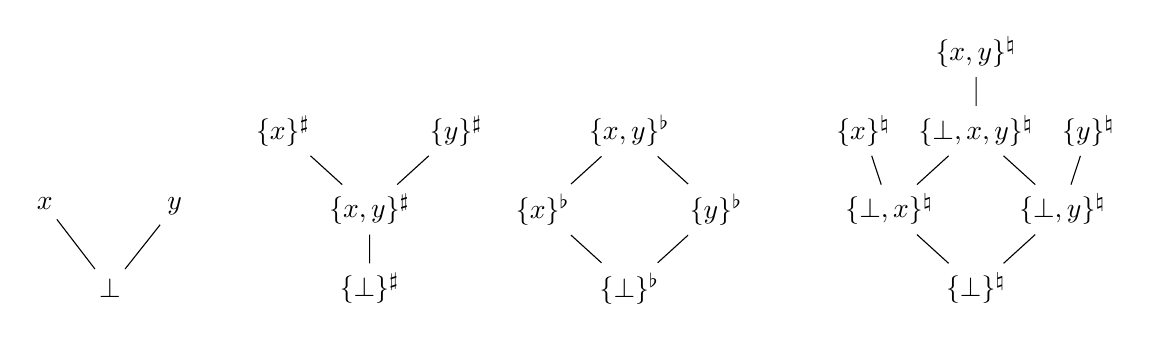
\begin{tikzpicture}[xscale=1.1]
  \node (U) at (0,0) {$\bot$};
  \node [anchor=base] (A) at (-0.75,1) {$x$};
  \node [anchor=base] (B) at (0.75,1) {$y$};
  \draw (A) -- (U) -- (B);
  
  \node (U1) at (3,0) {$\{\bot\}^\sharp$};
  \node (AB1) at (3,1) {$\{x,y\}^\sharp$};
  \node (A1) at (2,2) {$\{x\}^\sharp$};
  \node (B1) at (4,2) {$\{y\}^\sharp$};
  \draw (U1) -- (AB1);
  \draw (A1) -- (AB1) -- (B1);
  
  \node (U2) at (6,0) {$\{\bot\}^\flat$};
  \node (UA2) at (5,1) {$\{x\}^\flat$};
  \node (UAB2) at (6,2) {$\{x,y\}^\flat$};
  \node (UB2) at (7,1) {$\{y\}^\flat$};
  \draw (U2) -- (UA2) -- (UAB2);
  \draw (U2) -- (UB2) -- (UAB2);

  \node (U3) at (10,0) {$\{\bot\}^\natural$};
  \node (UA3) at (9,1) {$\{\bot,x\}^\natural$};
  \node (UB3) at (11,1) {$\{\bot,y\}^\natural$};
  \node (UAB3) at (10,2) {$\{\bot,x,y\}^\natural$};
  \node (A3) at (8.7,2) {$\{x\}^\natural$};
  \node (B3) at (11.3,2) {$\{y\}^\natural$};
  \node (AB3) at (10,3) {$\{x,y\}^\natural$};
  \draw (U3) -- (UA3) -- (A3);
  \draw (U3) -- (UB3) -- (B3);
  \draw (UA3) -- (UAB3);
  \draw (UB3) -- (UAB3);
  \draw (UAB3) -- (AB3);
\end{tikzpicture}
\par\end{centering}

\caption{Lifted two-element type, with upper, lower, and convex powerdomains}
\label{fig:lifted2}
\end{figure}


\begin{figure}
\begin{centering}
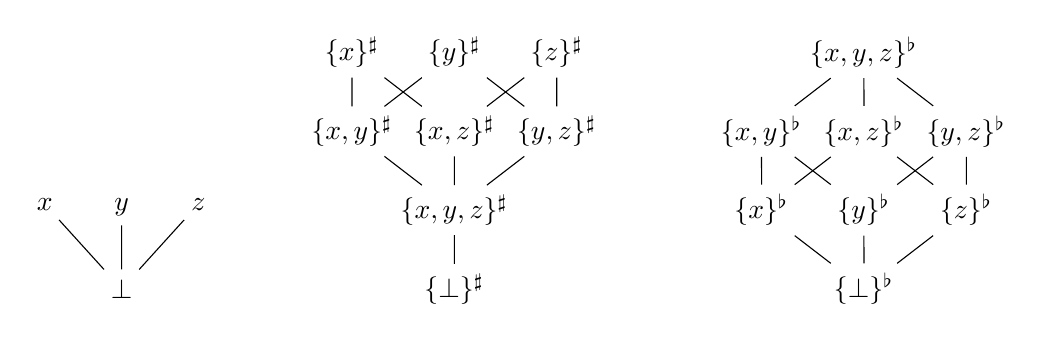
\begin{tikzpicture}[xscale=1.3]
  \node (U) at (0.75,0) {$\bot$};
  \node [anchor=base] (A) at (0,1) {$x$};
  \node [anchor=base] (B) at (0.75,1) {$y$};
  \node [anchor=base] (C) at (1.5,1) {$z$};
  \draw (U) -- (A);
  \draw (U) -- (B);
  \draw (U) -- (C);

  \node (U1) at (4,0) {$\{\bot\}^\sharp$};
  \node (ABC1) at (4,1) {$\{x,y,z\}^\sharp$};
  \node (AB1) at (3,2) {$\{x,y\}^\sharp$};
  \node (BC1) at (5,2) {$\{y,z\}^\sharp$};
  \node (CA1) at (4,2) {$\{x,z\}^\sharp$};
  \node (A1) at (3,3) {$\{x\}^\sharp$};
  \node (B1) at (4,3) {$\{y\}^\sharp$};
  \node (C1) at (5,3) {$\{z\}^\sharp$};
  \draw (U1) -- (ABC1);
  \draw (ABC1) -- (AB1) -- (A1) -- (CA1);
  \draw (ABC1) -- (BC1) -- (B1) -- (AB1);
  \draw (ABC1) -- (CA1) -- (C1) -- (BC1);

  \node (U2) at (8,0) {$\{\bot\}^\flat$};
  \node (UA2) at (7,1) {$\{x\}^\flat$};
  \node (UB2) at (8,1) {$\{y\}^\flat$};
  \node (UC2) at (9,1) {$\{z\}^\flat$};
  \node (UAB2) at (7,2) {$\{x,y\}^\flat$};
  \node (UBC2) at (9,2) {$\{y,z\}^\flat$};
  \node (UCA2) at (8,2) {$\{x,z\}^\flat$};
  \node (UABC2) at (8,3) {$\{x,y,z\}^\flat$};
  \draw (U2) -- (UA2) -- (UAB2);
  \draw (U2) -- (UB2) -- (UBC2);
  \draw (U2) -- (UC2) -- (UCA2);
  \draw (UA2) -- (UCA2) -- (UABC2);
  \draw (UB2) -- (UAB2) -- (UABC2);
  \draw (UC2) -- (UBC2) -- (UABC2);
\end{tikzpicture}
\par\end{centering}

\caption{Lifted three-element type, with upper and lower powerdomains}
\label{fig:lifted3}
\end{figure}


\begin{figure}
\begin{centering}
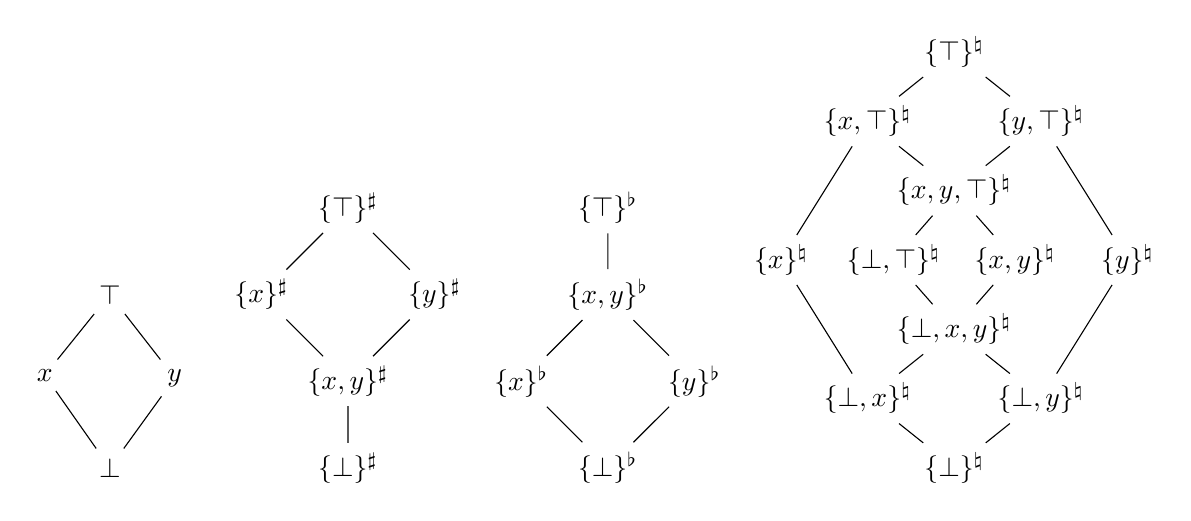
\begin{tikzpicture}[xscale=1.1, yscale=1.1]
  \node (U) at (1.25,0) {$\bot$};
  \node [anchor=base] (A) at (0.5,1) {$x$};
  \node [anchor=base] (B) at (2,1) {$y$};
  \node (T) at (1.25,2) {$\top$};
  \draw (U) -- (A) -- (T) -- (B) -- (U);
  
  \node (U1) at (4,0) {$\{\bot\}^\sharp$};
  \node (AB1) at (4,1) {$\{x,y\}^\sharp$};
  \node (A1) at (3,2) {$\{x\}^\sharp$};
  \node (B1) at (5,2) {$\{y\}^\sharp$};
  \node (T1) at (4,3) {$\{\top\}^\sharp$};
  \draw (U1) -- (AB1) -- (A1) -- (T1) -- (B1) -- (AB1);

  \node (U2) at (7,0) {$\{\bot\}^\flat$};
  \node (A2) at (6,1) {$\{x\}^\flat$};
  \node (B2) at (8,1) {$\{y\}^\flat$};
  \node (AB2) at (7,2) {$\{x,y\}^\flat$};
  \node (T2) at (7,3) {$\{\top\}^\flat$};
  \draw (T2) -- (AB2) -- (B2) -- (U2) -- (A2) -- (AB2);
  
  \node (U3) at (11,0) {$\{\bot\}^\natural$};
  \node (UA3) at (10,0.8) {$\{\bot,x\}^\natural$};
  \node (UB3) at (12,0.8) {$\{\bot,y\}^\natural$};
  \node (UAB3) at (11,1.6) {$\{\bot,x,y\}^\natural$};
  \node (A3) at (9,2.4) {$\{x\}^\natural$};
  \node (B3) at (13,2.4) {$\{y\}^\natural$};
  \node (UT3) at (10.3,2.4) {$\{\bot,\top\}^\natural$};
  \node (AB3) at (11.7,2.4) {$\{x,y\}^\natural$};
  \node (ABT3) at (11,3.2) {$\{x,y,\top\}^\natural$};
  \node (AT3) at (10,4.0) {$\{x,\top\}^\natural$};
  \node (BT3) at (12,4.0) {$\{y,\top\}^\natural$};
  \node (T3) at (11,4.8) {$\{\top\}^\natural$};
  \draw (U3) -- (UA3) -- (UAB3);
  \draw (U3) -- (UB3) -- (UAB3);
  \draw (UA3) -- (A3) -- (AT3);
  \draw (UB3) -- (B3) -- (BT3);
  \draw (UAB3) -- (UT3) -- (ABT3);
  \draw (UAB3) -- (AB3) -- (ABT3);
  \draw (ABT3) -- (AT3) -- (T3);
  \draw (ABT3) -- (BT3) -- (T3);
\end{tikzpicture}
\par\end{centering}
\caption{Four-element lattice, with upper, lower, and convex powerdomains}
\label{fig:lattice4}
\end{figure}


\section{Powerdomain library features}
\label{sec:HOLCF-powerdomain-library}

This section describes the user-visible aspects of the HOLCF powerdomain library. The implementation defines three new type constructors, one for each of the three powerdomain varieties. Each type has \isa{unit} and \isa{plus} constructors, and a monadic \isa{bind} operator. Each type also has \isa{map} and \isa{join} operators, defined in terms of \isa{unit} and \isa{bind} in the same manner as Haskell's \texttt{liftM} and \texttt{join}. The full list of types and constants is shown in Fig. \ref{fig:type-signatures}.

The functions \isa{convex_to_lower} and \isa{convex_to_upper} are the mappings guaranteed to exist by the universal property of the convex powerdomain; they preserve \isa{unit} and \isa{plus}. Note that instead of the full function space (\isa{=>}), all functions use the HOLCF continuous function space type (\isa{->}), indicating that they are continuous functions.

\begin{figure}
\indexdef{upper_unit}
\indexdef{upper_plus}
\indexdef{upper_bind}
\indexdef{upper_map}
\indexdef{upper_join}
\begin{isacode}
upper_unit :: 'a -> 'a upper_pd
upper_plus :: 'a upper_pd -> 'a upper_pd -> 'a upper_pd
upper_bind :: 'a upper_pd -> ('a -> 'b upper_pd) -> 'b upper_pd
upper_map :: ('a -> 'b) -> 'a upper_pd -> 'b upper_pd
upper_join :: 'a upper_pd upper_pd -> 'a upper_pd
\end{isacode}
\unmedskip
\indexdef{lower_unit}
\indexdef{lower_plus}
\indexdef{lower_bind}
\indexdef{lower_map}
\indexdef{lower_join}
\begin{isacode}
lower_unit :: 'a -> 'a lower_pd
lower_plus :: 'a lower_pd -> 'a lower_pd -> 'a lower_pd
lower_bind :: 'a lower_pd -> ('a -> 'b lower_pd) -> 'b lower_pd
lower_map :: ('a -> 'b) -> 'a lower_pd -> 'b lower_pd
lower_join :: 'a lower_pd lower_pd -> 'a lower_pd
\end{isacode}
\unmedskip
\indexdef{convex_unit}
\indexdef{convex_plus}
\indexdef{convex_bind}
\indexdef{convex_map}
\indexdef{convex_join}
\begin{isacode}
convex_unit :: 'a -> 'a convex_pd
convex_plus :: 'a convex_pd -> 'a convex_pd -> 'a convex_pd
convex_bind :: 'a convex_pd -> ('a -> 'b convex_pd) -> 'b convex_pd
convex_map :: ('a -> 'b) -> 'a convex_pd -> 'b convex_pd
convex_join :: 'a convex_pd convex_pd -> 'a convex_pd
\end{isacode}
\unmedskip
\indexdef{convex_to_upper}
\indexdef{convex_to_lower}
\begin{isacode}
convex_to_upper :: 'a convex_pd -> 'a upper_pd
convex_to_lower :: 'a convex_pd -> 'a lower_pd
\end{isacode}

\caption{Powerdomain constants defined in \HOLCF{11}}
\label{fig:type-signatures}
\end{figure}

For convenience, the library also provides set-style syntax for powerdomain operations: We can write \isa{\<lbrace>x\<rbrace>\<sharp>} for \isa{upper_unit\<cdot>x}, \isa{xs \<union>\<sharp> ys} for \isa{upper_plus\<cdot>xs\<cdot>ys}, \isa{\<Union>\<sharp>x\<in>xs. t} for \isa{upper_bind\<cdot>xs\<cdot>(\<Lambda> x. t)}, and so on for the other powerdomain types.

Along with the definitions of types and constants, the library provides a significant body of lemmas, many of which are declared to the simplifier. Each powerdomain type has an induction rule in terms of \isa{unit} and \isa{plus}, similar to Eq.~(\ref{eq:pd-induct}). Rules about injectivity, strictness, compactness, and ordering are provided for the constructors. Rewrite rules are provided for the \isa{bind}, \isa{map}, and \isa{join} functions applied to \isa{unit}, \isa{plus}, or \isa{\<bottom>}. All of the powerdomain laws are also included as lemmas.


\subsection{Type class constraints}
\label{sec:pd-class-constraint}

The main axiomatic type classes in HOLCF are \isa{cpo} (chain-complete partial orders) and \isa{pcpo} (pointed cpos). Unfortunately, the powerdomain constructions do not work over arbitrary cpos; they need some additional structure. To formalize powerdomains in HOLCF, it was necessary to add a new axiomatic class \isa{bifinite}, which is a subclass of \isa{pcpo}. All of the functions defined in the \HOLCF{11} powerdomain theories have a \isa{bifinite} class constraint. The definition and relevant properties of class \isa{bifinite} will be discussed in Section \ref{sec:pd-bifinite}.

As far as a user of the library is concerned, it does not matter how class \isa{bifinite} is defined; the important thing is that it should be preserved by all of type constructors that the user works with. \HOLCF{11} provides \isa{bifinite} class instances for all of its type constructors: continuous function space, cartesian product, strict product, strict sum, lifted cpos, and all three varieties of powerdomains. Flat domains built from countable HOL types are also instances of \isa{bifinite}. The \textsc{Domain} package also generates instances of the \isa{bifinite} class, when it is used in its definitional mode (see Chapter~\ref{ch:universal}).


\subsection{Automation}

To facilitate reasoning with powerdomains, the library provides various sets of rewrite rules that are designed to work well together.

\paragraph{ACI normalization.} Isabelle's simplifier is set up to handle permutative rewrite rules, which are equations like $x+y=y+x$ whose right and left-hand-sides are the same modulo renaming of variables \cite{isabelle-tutorial}. For any associative-commutative (AC) operator, there is a set of three permutative rewrite rules that can convert any expression built from the operator into a normal form (grouped to the right, with terms sorted according to some syntactic term-ordering) \cite{baader1998}. Two of the AC rewrites are simply the associativity and commutativity rules. The third is the left-commutativity rule. For normalizing an associative-commutative-idempotent (ACI) operator, we need a total of five rules: the three AC rewrites, plus the idempotency rule, and also (analogous to left-commutativity) left-idempotency.
\begin{eqnarray}
(xs\cup ys)\cup zs & = & xs\cup(ys\cup zs)\nonumber \\
ys\cup xs & = & xs\cup ys\nonumber \\
ys\cup(xs\cup zs) & = & xs\cup(ys\cup zs)\label{eq:plus-aci}\\
xs\cup xs & = & xs\nonumber \\
xs\cup(xs\cup ys) & = & xs\cup ys\nonumber
\end{eqnarray}

Permutative rewriting using the ACI rules results in a normal form where expressions are nested to the right, and the terms are sorted according to the syntactic term ordering, with no exact duplicates. In \HOLCF{11}, this normalization can be accomplished for the convex powerdomains by invoking the simplifier with \isa{simp add: convex_plus_aci}. Similarly, \isa{upper_plus_aci} and \isa{lower_plus_aci} may be used with upper and lower powerdomains, respectively.


\paragraph{Solving inequalities.} A common subgoal in a proof might be to show that one powerdomain expression is below another. For each variety of powerdomain, there is a set of rewrite rules that can automatically reduce an inequality on powerdomains down to inequalities on the underlying type.
\begin{eqnarray}
\{x\}^{\sharp}\sqsubseteq\{y\}^{\sharp} & \iff & x\sqsubseteq y\nonumber \\
xs\sqsubseteq(ys\cup^{\sharp}zs) & \iff & (xs\sqsubseteq ys)\wedge(xs\sqsubseteq zs)\label{eq:upper-less}\\
(xs\cup^{\sharp}ys)\sqsubseteq\{z\}^{\sharp} & \iff & (xs\sqsubseteq\{z\}^{\sharp})\vee(ys\sqsubseteq\{z\}^{\sharp})\nonumber
\end{eqnarray}
\begin{eqnarray}
\{x\}^{\flat}\sqsubseteq\{y\}^{\flat} & \iff & x\sqsubseteq y\nonumber \\
(xs\cup^{\flat}ys)\sqsubseteq zs & \iff & (xs\sqsubseteq zs)\wedge(ys\sqsubseteq zs)\label{eq:lower-less}\\
\{x\}^{\flat}\sqsubseteq(ys\cup^{\flat}zs) & \iff & (\{x\}^{\flat}\sqsubseteq ys)\vee(\{x\}^{\flat}\sqsubseteq zs)\nonumber
\end{eqnarray}
\begin{eqnarray}
\{x\}^{\natural}\sqsubseteq\{y\}^{\natural} & \iff & x\sqsubseteq y\nonumber \\
\{x\}^{\natural}\sqsubseteq(ys\cup^{\natural}zs) & \iff & (\{x\}^{\natural}\sqsubseteq ys)\wedge(\{x\}^{\natural}\sqsubseteq zs)\label{eq:convex-less}\\
(xs\cup^{\natural}ys)\sqsubseteq\{z\}^{\natural} & \iff & (xs\sqsubseteq\{z\}^{\natural})\wedge(ys\sqsubseteq\{z\}^{\natural})\nonumber
\end{eqnarray}

For the upper and lower powerdomains, each has a set of three rewrite rules that covers all cases of comparisons. For example, \isa{simp add: upper_pd_below_simps} will rewrite \isa{\<lbrace>x, y\<rbrace>\<sharp> \<sqsubseteq> \<lbrace>y, z\<rbrace>\<sharp>} into \isa{x \<sqsubseteq> z \<or> y \<sqsubseteq> z}, using the rules in Eq.~(\ref{eq:upper-less}). Similarly, simplification with \isa{lower_pd_below_simps} uses the rules in Eq.~(\ref{eq:lower-less}) to simplify inequalities on lower powerdomains.

For the convex powerdomain, the three rules in Eq.~(\ref{eq:convex-less}) are incomplete: They do not cover the case of $(xs\cup^{\natural}ys)\sqsubseteq(zs\cup^{\natural}ws)$. To handle this case, we will take advantage of the coercions from the convex powerdomain to the upper and lower powerdomains, along with the following ordering property:
%
\indexthm{convex_pd_below_iff}
\begin{isacode}
lemma convex_pd_below_iff:
  "(xs \<sqsubseteq> ys) <->
      (convex_to_upper\<cdot>xs \<sqsubseteq> convex_to_upper\<cdot>ys \<and>
        convex_to_lower\<cdot>xs \<sqsubseteq> convex_to_lower\<cdot>ys)"
\end{isacode}
%
The rule set \isa{convex_pd_below_simps} includes all rules from Eqs.~(\ref{eq:upper-less})--(\ref{eq:convex-less}), and a suitably instantiated \isa{convex_pd_below_iff} to cover the missing case.

\paragraph{Using inequalities to solve non-trivial equalities.} The ACI rewriting can take care of many equalities between powerdomain expressions, but the inequality rules can actually solve more. For example, using the assumptions $x \sqsubseteq y$ and $y \sqsubseteq z$, we will prove that $\{x, y, z\}^\natural = \{x, z\}^\natural$. By antisymmetry, we can rewrite this to the conjunction $(\{x,y,z\}^{\natural}\sqsubseteq\{x,z\}^{\natural})\wedge(\{x,z\}^{\natural}\sqsubseteq\{x,y,z\}^{\natural})$. Next, we can simplify with \isa{convex_pd_below_simps}, and this subgoal reduces to $(y\sqsubseteq x\vee y\sqsubseteq z)\wedge(x\sqsubseteq y\vee z\sqsubseteq y)$. Finally, this is easily discharged using the assumptions $x\sqsubseteq y$ and $y\sqsubseteq z$.


\section{Ideal completion}
\label{sec:pd-ideal-completion}

In Chapter~\ref{ch:holcf}, we defined various basic HOLCF types as subsets of other cpos, using the \textsc{Cpodef} package. Unfortunately, this is not possible for powerdomains. In such cases where \textsc{Cpodef} is not applicable, we want to minimize the proof effort for proving the completeness axioms and continuity of operations. One way to accomplish this is to define a cpo using \emph{ideal completion}.

The powerdomain construction used in HOLCF makes use of an alternative representation of cpos, where we just consider the set of compact (i.e., finite) values, rather than the whole cpo~\cite[\S2.2.6]{abramsky94domain}. (Refer to Sec.~\ref{sec:holcf-fix} for the HOLCF definition and properties of compactness.) For a certain class of cpos, called \emph{algebraic} cpos, every value can be expressed as the least upper bound of its compact approximants. This means that in an algebraic cpo $D$ the set of compact elements $K(D)$, together with the ordering on them, fully represents the entire cpo. We say that $K(D)$ forms a \emph{basis} for the cpo $D$, and that the entire cpo $D$ is a \emph{completion} of the basis.

To construct a new algebraic cpo by ideal completion, we can start by defining its basis. The ordering on the basis can be any partial order, not necessarily a complete partial order. The operations on the basis only need to be monotone, not necessarily continuous. (This is helpful because monotonicity is generally much easier to prove than continuity.)  The ideal completion process extends the basis with new infinite elements to give a cpo. Similarly, a process called \emph{continuous extension} lifts the monotone operations on the basis up to continuous functions on the new cpo.

The ideal completion process is formalized as a library in \HOLCF{11}; this section will describe the formalization, and show how to define new cpo types with it. Section~\ref{sec:pd-implementation} shows how it is used to define the powerdomain type constructors. The process is general enough to be useful for other cpos besides powerdomains; Chapter~\ref{ch:universal} will show how it is used to construct a universal domain.

\subsection{Preorders and ideals}

A \emph{preorder} is defined as a binary relation that is reflexive and transitive. Given a basis with a preorder relation $\left\langle B,\preceq\right\rangle$, we can construct an algebraic cpo by ideal completion. This is done by considering the set of ideals over the basis:

\begin{definition}
A set $S \subseteq B$ is an \emph{ideal} with respect to preorder relation
$(\preceq)$ if it has the following properties:
\begin{itemize*}
\item $S$ is nonempty: $\exists x.\: x\in S$
\item $S$ is downward-closed: $\forall x\: y.\: x\preceq y\longrightarrow y\in S\longrightarrow x\in S$
\item $S$ is directed (i.e., has an upper bound for any pair of elements):\\
 $\forall x\: y.\: x\in S\longrightarrow y\in S\longrightarrow(\exists z.\: z\in S\wedge x\preceq z\wedge y\preceq z)$
\end{itemize*}
A \emph{principal} \emph{ideal} is an ideal of the form $\{y \mid y\preceq x\}$ for some $x$, written $\downarrow\! x$.
\end{definition}
The set of all ideals over $\left\langle B,\preceq\right\rangle $ is denoted by $\mathrm{Idl}(B)$; when ordered by subset inclusion, $\mathrm{Idl}(B)$ forms an algebraic cpo. The compact elements of $\mathrm{Idl}(B)$ are exactly those represented by principal ideals. The algebraicity of $\mathrm{Idl}(B)$ is manifest in the following induction rule: For an admissible predicate $P$, if $P$ holds for all principal ideals, then it holds for all elements of $\mathrm{Idl}(B)$.
%
\begin{equation}
\inferrule
  {\mathrm{adm}(P) \\ \forall x \in B.\:P(\downarrow\! x)}
  {\forall y \in \mathrm{Idl}(B).\:P(y)}
\label{eq:ideal-induct}
\end{equation}
%
(If the notion of admissibility is defined using directed sets, then Eq.~\eqref{eq:ideal-induct} holds for any preordered basis $B$. But if admissibility is defined using countable chains---as it is in HOLCF---then we must require the basis $B$ to be a countable set.)

Note that we do not require $(\preceq)$ to be antisymmetric. For $x$ and $y$ that are equivalent (that is, both $x\preceq y$ and $y\preceq x$) the principal ideals $\downarrow\! x$ and $\downarrow\! y$ are equal. This means that the ideal completion construction automatically quotients by the equivalence induced by $(\preceq)$.

\subsection{Formalizing ideal completion}
\label{sec:pd-completion-formalize}

%Ideal completion is formalized using Isabelle's locale mechanism~\cite{KWP99locales, Ballarin10}. A \emph{locale} is essentially like a named proof context: It fixes parameters and collects assumptions about them. Lemmas can be proved \emph{in} a locale, where the assumptions of the locale become extra implicit hypotheses. Likewise, constants can be defined in a locale, and the locale parameters become extra implicit arguments. Locales can then be \emph{interpreted} by instantiating the parameters with values that satisfy the assumptions, generating customized versions of all the constants and lemmas from the locale.
Ideal completion is formalized using Isabelle's locale mechanism~\cite{KWP99locales, Ballarin10}. A \emph{locale} is like a named proof context: It fixes parameters and collects assumptions about them. Lemmas can be proved \emph{in} a locale, where the assumptions of the locale become extra implicit hypotheses. Likewise, constants can be defined in a locale, with the locale parameters as extra implicit arguments. Locales can be \emph{interpreted} by instantiating the parameters with values that satisfy the assumptions, generating specialized versions of all the constants and lemmas from the locale.

Locales are similar in some ways to axiomatic type classes. Both of these mechanisms are used to formalize algebraic structures, which involve some number of fixed operations and assumptions about them. However, each mechanism has its own strengths and limitations, and some situations require one or the other. The formalization of ideal completion relies on two features unique to locales: First, while a type class may only mention a single type variable, locales may be parameterized by any number of types. This feature is necessary because ideal completion relates two types: a basis and a completed cpo. Second, locales allow multiple interpretations at the same type---unlike type classes, which only allow one instantiation per type. This feature allows us to define multiple preorders and ideal completions with the same basis type.


\paragraph{Locale for preorders.} The \HOLCF{11} ideal completion library defines two locales, \isa{preorder} and \isa{ideal_completion}; we will discuss the \isa{preorder} locale first. The \isa{preorder} locale fixes a type \isa{'a} corresponding to the basis $B$, and a preorder relation \isa{\<preceq>} on that type. We also define a predicate \isa{ideal} within the locale.
%
\indexdef{preorder}
\begin{isacode}
locale preorder =
  fixes r :: "'a::type => 'a => bool" (infix "\<preceq>" 50)
  assumes r_refl: "x \<preceq> x"
  assumes r_trans: "[|x \<preceq> y; y \<preceq> z|] ==> x \<preceq> z"
\end{isacode}
\unmedskip
\indexdef{ideal}
\begin{isacode}
definition (in preorder) ideal :: "'a set => bool"
  where "ideal A \<longleftrightarrow>
    (\<exists>x. x \<in> A) \<and> (\<forall>x\<in>A. \<forall>y\<in>A. \<exists>z\<in>A. x \<preceq> z \<and> y \<preceq> z) \<and>
    (\<forall>x y. x \<preceq> y --> y \<in> A --> x \<in> A)"
\end{isacode}
%
Within the \isa{preorder} locale, we prove that principal ideals are indeed ideals. We also prove that the union of a chain of ideals is itself an ideal---which shows that the ideal completion is a cpo.
%
\indexthm{ideal_principal}
\begin{isacode}
lemma (in preorder) ideal_principal:
  shows "ideal {x. x \<preceq> z}"
\end{isacode}
\unmedskip
\indexthm{ideal_UN}
\begin{isacode}
lemma (in preorder) ideal_UN:
  fixes A :: "nat => 'a set"
  assumes ideal_A: "\<And>i. ideal (A i)"
  assumes chain_A: "\<And>i j. i \<le> j ==> A i \<subseteq> A j"
  shows "ideal (\<Union>i. A i)"
\end{isacode}
%
Next we shall consider the steps required to define a new cpo in Isabelle using ideal completion. The first step is to choose a type to use as a basis and define a preorder relation on it. For example, as a basis we might use lists of natural numbers, with a prefix ordering (\isa{@} is Isabelle's list-append operator). After defining the relation we proceed to interpret the \isa{preorder} locale.
%
\indexdefx{prefix}
\begin{isacode}
definition prefix :: "nat list => nat list => bool"
  where "prefix xs ys = (\<exists>zs. ys = xs @ zs)"
\end{isacode}
\unmedskip
\begin{isacode}
interpretation preord_prefix: preorder prefix
  by ...
\end{isacode}
%
The interpretation command requires a proof that \isa{prefix} satisfies the assumptions of the locale---in this case, reflexivity and transitivity. After we discharge the proof obligations, the locale package generates copies of all constants and lemmas from the \isa{preorder} locale, instantiated with \isa{prefix} in place of \isa{\<preceq>} and with the qualifier ``\isa{preord_prefix}'' prepended to all the names.

The next step is to define a new type as the set of ideals over the basis, using \textsc{Typedef}. (Recall that the \isa{open} option serves merely to prevent \textsc{Typedef} from defining an unneeded set constant called \isa{inflist}.) The non-emptiness obligation can be discharged using lemma \isa{preord_prefix.ideal_principal}.
%
\begin{isacode}
typedef (open) inflist = "{S::nat list set. preord_prefix.ideal S}"
\end{isacode}
%
After defining the type, we define the ordering \isa{(\<sqsubseteq>)} on type \isa{inflist} in terms of the subset ordering on type \isa{nat list set}.
%
\indexthmx{below_inflist_def}
\begin{isacode}
instantiation inflist :: below
begin
  definition below_inflist_def: "(x \<sqsubseteq> y) = (Rep_inflist x \<subseteq> Rep_inflist y)"
  instance ..
end
\end{isacode}
%
We still need to prove that \isa{inflist} is an instance of the \isa{po} and \isa{cpo} classes. For this purpose, the ideal completion library provides a pair of lemmas that are very similar to those used by the \textsc{Cpodef} package from Chapter~\ref{ch:holcf} (\S\ref{sec:holcf-cpodef}). They have assumptions about the \isa{type_definition} predicate, and their conclusions are \isa{OFCLASS} predicates.
%
\indexthm{typedef_ideal_po}
\begin{isacode}
lemma (in preorder) typedef_ideal_po:
  fixes Rep :: "'b::below => 'a set'' and Abs :: "'a set => 'b"
  assumes type: "type_definition Rep Abs {S. ideal S}"
  assumes below: "\<And>x y. x \<sqsubseteq> y \<longleftrightarrow> Rep x \<subseteq> Rep y"
  shows "OFCLASS('b, po_class)"
\end{isacode}
\unmedskip
\indexthm{typedef_ideal_cpo}
\begin{isacode}
lemma (in preorder) typedef_ideal_cpo:
  fixes Rep :: "'b::po => 'a set'' and Abs :: "'a set => 'b"
  assumes type: "type_definition Rep Abs {S. ideal S}"
  assumes below: "\<And>x y. x \<sqsubseteq> y \<longleftrightarrow> Rep x \<subseteq> Rep y"
  shows "OFCLASS('b, cpo_class)"
\end{isacode}
%
The proof of \isa{typedef_ideal_po} is straightforward. To prove \isa{typedef_ideal_cpo}, we show that \isa{Abs (\<Union>i. Rep (Y i))} gives the least upper bound for any chain \isa{Y}.

Using lemma \isa{type_definition_inflist} (provided by \textsc{Typedef}) and \isa{below_inflist_def} together with \isa{preord_prefix.typedef_ideal_po} and \isa{preord_prefix.typedef_ideal_cpo}, we can prove the \isa{po} and \isa{cpo} class instances for \isa{inflist}.

\paragraph{Locale for ideal completions.} Having defined a cpo with ideal completion, we can now define an embedding from the basis type into the completion type, using principal ideals.
%
\indexdefx{principal_inflist}
\begin{isacode}
definition principal_inflist :: "nat list => inflist"
  where "principal_inflist x = Abs_inflist {a. prefix a x}"
\end{isacode}
%
In order to prove generic theorems about this embedding, HOLCF defines another locale on top of the \isa{preorder} locale, called \isa{ideal_completion}. In addition to type \isa{'a} representing the basis $B$, the new locale fixes another type \isa{'b} corresponding to $\mathrm{Idl}(B)$. It fixes two new functions: \isa{rep} returns the representation of a value as a set of basis elements, generalizing the function \isa{Rep_inflist}; and \isa{principal} returns values that correspond to principal ideals, generalizing \isa{principal_inflist}.
%
\indexdef{ideal_completion}
\begin{isacode}
locale ideal_completion = preorder +
  fixes principal :: "'a::type \<Rightarrow> 'b::cpo"
  fixes rep :: "'b::cpo \<Rightarrow> 'a::type set"
  assumes ideal_rep: "\<And>x. ideal (rep x)"
  assumes rep_lub: "\<And>Y. chain Y \<Longrightarrow> rep (\<Squnion>i. Y i) = (\<Union>i. rep (Y i))"
  assumes rep_principal: "\<And>a. rep (principal a) = {b. b \<preceq> a}"
  assumes belowI: "\<And>x y. rep x \<subseteq> rep y \<Longrightarrow> x \<sqsubseteq> y"
  assumes countable: "\<exists>f::'a \<Rightarrow> nat. inj f"
\end{isacode}
%
The assumptions of the \isa{ideal_completion} locale are designed to be easily satisfied by types like \isa{inflist} that are defined by ideal completion over a countable basis type. To assist with \isa{ideal_completion} locale interpretation proofs, the library provides the following lemma:
%
\indexthm{typedef_ideal_completion}
\begin{isacode}
lemma (in preorder) typedef_ideal_completion:
  fixes Rep :: "'b::cpo => 'a set" and Abs :: "'a set => 'b"
  assumes type: "type_definition Rep Abs {S. ideal S}"
  assumes below: "\<And>x y. x \<sqsubseteq> y \<longleftrightarrow> Rep x \<subseteq> Rep y"
  assumes principal: "\<And>a. principal a = Abs {b. b \<preceq> a}"
  assumes countable: "\<exists>f::'a \<Rightarrow> nat. inj f"
  shows "ideal_completion r principal Rep"
\end{isacode}
%
Within the \isa{ideal_completion} locale, we start by proving a few simple lemmas about \isa{principal}: The ordering between principal values reflects the basis ordering, and every principal value is compact.
%
\indexthm{principal_below_iff}
\begin{isacode}
lemma (in ideal_completion) principal_below_iff [simp]:
  "principal a \<sqsubseteq> principal b <-> a \<preceq> b"
\end{isacode}
\unmedskip
\indexthm{compact_principal}
\begin{isacode}
lemma (in ideal_completion) compact_principal [simp]:
  "compact (principal a)"
\end{isacode}
%
Perhaps the most important theorem in the \isa{ideal_completion} locale, however, is the principal induction rule given in Eq.~\eqref{eq:ideal-induct}. In order to help prove it, we must start with a lemma related to the countability of the basis: Any value in the complete cpo can be expressed as the least upper bound of a chain of principal values.
%
\indexthm{obtain_principal_chain}
\begin{isacode}
lemma (in ideal_completion) obtain_principal_chain:
  "\<exists>Y. (\<forall>i. Y i \<preceq> Y (Suc i)) \<and> x = (\<Squnion>i. principal (Y i))"
\end{isacode}
%
The proof proceeds by explicitly constructing such a chain, following a technique from the proof of Proposition 2.2.14 in Abramsky and Jung \cite{abramsky94domain}. Let $(b_n)_{n\in\omega}$ be an enumeration of the basis $B$, and let $x$ be a value in the completion represented by the ideal $S$. Then we can construct a sequence of basis values $(s_i)_{i\in\omega}$ as follows. Let $s_0$ be the first $b_n$ such that $b_n \in S$. Then for every $i\in\omega$ we define $t_i$ as the first $b_n$ such that $b_n \in S$ and $b_n \not\preceq s_i$. Then we inductively define $s_{i+1}$ as the first $b_n$ in $S$ above both $s_i$ and $t_i$. It can be shown that the sequence $s_i$ yields the desired least upper bound.

Using lemma \isa{obtain_principal_chain}, the principal induction rule follows directly.
%
\vspace{-22pt} % FUDGE
\indexthm{principal_induct}
\begin{isacode}
lemma (in ideal_completion) principal_induct:
  "[|adm P; !!a. P (principal a)|] ==> P x"
\end{isacode}
%
As we will see later in Sec.~\ref{sec:pd-implementation}, induction over principal values is the primary way to transfer properties about the basis type up to the completed cpo. Lemma \isa{principal_induct} is used dozens of times in the proof scripts of the \HOLCF{11} powerdomain theories.

\subsection{Continuous extensions of functions}

A continuous function on an algebraic cpo is completely determined by its action on compact elements. This suggests a method for defining continuous functions over ideal completions: First, define a function from the basis $B$ to a cpo $C$ such that $f$ is monotone, i.e., $x\preceq y$ implies $f(x)\sqsubseteq f(y)$. Then there exists a unique function $\widehat{f}:\mathrm{Idl}(B)\rightarrow C$ that agrees with $f$ on principal ideals, i.e., for all $x$, $\widehat{f}(\downarrow\! x)=f(x)$. We say that $\widehat{f}$ is the \emph{continuous extension} of $f$.

The continuous extension is defined by mapping the function $f$ over the input ideal, and then taking the least upper bound of the resulting directed set: $\widehat{f}(S)=\bigsqcup_{x\in S}f(x)$. Generally, the result type $C$ would need to be a directed-complete partial order\footnote{Directed-completeness means that every directed set has a least upper bound. This is a stronger condition than chain-completeness, which is used in the HOLCF formalization of cpos.} to ensure that this least upper bound exists. However, if the basis $B$ is countable, then it is possible to find a chain in $S$ that yields the same least upper bound as $S$. This means that $C$ can be any chain-complete partial order.

\subsection{Formalizing continuous extensions}

Within the \isa{ideal_completion} locale we define a function \isa{extension}, which takes a monotone function $f$ as an argument, and returns the continuous extension $\widehat{f}$.
%
\indexdef{extension}
\begin{isacode}
definition (in ideal_completion) extension :: "('a \<Rightarrow> 'c::cpo) \<Rightarrow> ('b \<rightarrow> 'c)"
  where "extension f = (\<Lambda> x. lub (image f (rep x)))"
\end{isacode}
%
The definition of \isa{extension} uses two features that are only well-defined if certain conditions are met: First, the function \isa{lub} requires that its argument actually have a least upper bound. Second, the continuous function abstraction requires that the body be continuous in \isa{x}. Both of these properties rely on the monotonicity of \isa{f}.

To prove that \isa{image f (rep x)} has a least upper bound, we use the lemma \isa{obtain_principal_chain} to get a chain \isa{Y :: nat => 'a} of basis elements such that \isa{x =} \isa{(\<Squnion>i. principal (Y i))}. Then we show that \isa{(\<Squnion>i. f (Y i))} is the desired least upper bound. The continuity of the abstraction then follows from \isa{rep_lub} combined with properties of least upper bounds. Finally, we can establish the behavior of \isa{extension} on principal ideals, using the fact that \isa{f a} is a least upper bound of the set \isa{image f (rep (principal a))}.
%
\indexthm{extension_principal}
\begin{isacode}
lemma extension_principal:
  assumes f_mono: "\<And>a b. a \<preceq> b \<Longrightarrow> f a \<sqsubseteq> f b"
  shows "extension f\<cdot>(principal a) = f a"
\end{isacode}
%
To prove a property about a function defined as a continuous extension, the general approach is to use principal induction (lemma \isa{principal_induct}) to reduce the general subgoal to one about principal values; then lemma \isa{extension_principal} can be used to unfold the definition.

\section{Bifinite cpos}
\label{sec:pd-bifinite}

The construction used here for powerdomains only works with element types that are algebraic cpos, having bases of compact elements. As was mentioned earlier in Sec.~\ref{sec:pd-class-constraint}, the type classes \isa{cpo} and \isa{pcpo} are not sufficient to meet this requirement. Instead, the powerdomain libraries are based on the \isa{bifinite} class, which is a subclass of \isa{pcpo}.
%
\begin{definition}
A continuous function $f : D \to D$ is a \emph{deflation} if it is idempotent and below the identity function: $f \circ f = f \sqsubseteq \mathrm{Id}_D$. A \emph{finite deflation} is a deflation whose image is a finite set.
\end{definition}
%
\begin{definition}
Let $D$ be a cpo, and let $\mathcal{M}$ be the set of finite deflations over $D$. Then we say that $D$ is \emph{bifinite} if $\mathcal{M}$ is countable and directed with $\bigsqcup \mathcal{M} = \mathrm{Id}_D$.
\end{definition}

Given a deflation $f$ over a cpo $D$, the image of $f$ identifies a sub-cpo of $D$. Similarly, a finite deflation over $D$ identifies a finite poset that is a subset of $K(D)$. Intuitively then, a bifinite cpo is one that can be expressed as the limit (in an appropriate sense) of a countable collection of finite posets.

A few notes on terminology: The definitions of ``deflation'' and ``finite deflation'' used here were taken from Gunter \cite[\S3.1]{gunter85thesis}. Deflations are also commonly known as ``projections'' or sometimes ``kernel operators'' \cite{abramsky94domain}. Abramsky and Jung also use the term ``idempotent deflation'' to refer to finite deflations \cite{abramsky94domain}. We include a countability requirement in the definition of bifiniteness, following Gunter and Scott \cite{gunter90semantic}. Some authors \cite{abramsky94domain} relax this requirement, allowing bifinite domains of arbitrary cardinality, and using the qualifiers ``countably based'' or ``$\omega$-bifinite'' as required. Bifinite domains were originally defined by Plotkin as limits of expanding sequences of finite posets, who used the name ``SFP domains''~\cite{plotkin76powerdomain}.

Many categories of cpos can be found in the domain theory literature \cite{amadio+curien, gunter90semantic, abramsky94domain}. Of all the possibilities, the bifinites were chosen because they meet the following criteria:
%
\begin{itemize}
\item All bifinite cpos are algebraic: Every bifinite type has a basis of compact elements, given by the union of the ranges of the finite deflations.
\item In bifinite cpos, every directed set contains a countable chain with the same limit. This means that for bifinite cpos, the notions of directed-continuity and chain-continuity coincide. This is important for fitting the ideal completion construction (which uses directed sets) into HOLCF (which defines everything with chains).
\item The class of bifinite cpos is closed under all type constructors used in HOLCF, including all three powerdomains.
\item A universal bifinite domain exists, which can be used to represent general recursive data\-types (see Chapter~\ref{ch:universal}).
\end{itemize}
%
The requirement for algebraicity rules out the chain-complete cpos (classes \isa{cpo} and \isa{pcpo}). The category of countably-based algebraic cpos meets the first two criteria, but it fails the third: The continuous function space between two arbitrary algebraic cpos is not necessarily algebraic. The category of bounded-complete domains (also known as ``Scott domains'') meets nearly all of the criteria, including having a universal domain---except that bounded-completeness fails to be preserved by the convex powerdomain \cite{gunter90semantic}.

\subsection{Type class for bifinite cpos}

Next we will see how the class \isa{bifinite} is defined in \HOLCF{11}. We start by defining \isa{deflation} and \isa{finite_deflation}. Defining them as locales makes it more convenient to prove numerous simple lemmas about deflations and finite deflations.
%
\indexdef{deflation}
\indexthm{deflation.idem}
\indexthm{deflation.below}
\begin{isacode}
locale deflation =
  fixes d :: "'a \<rightarrow> 'a"
  assumes idem: "\<And>x. d\<cdot>(d\<cdot>x) = d\<cdot>x"
  assumes below: "\<And>x. d\<cdot>x \<sqsubseteq> x"
\end{isacode}
\unmedskip
\indexdef{finite_deflation}
\indexthm{finite_fixes}
\begin{isacode}
locale finite_deflation = deflation +
  assumes finite_fixes: "finite {x. d\<cdot>x = x}"
\end{isacode}
%
Note that \isa{finite_deflation} is defined using the set of fixed points of \isa{d}, rather than the image of \isa{d}; it is provable within the \isa{deflation} locale that these sets are equal. This formulation makes it slightly easier to prove that particular functions are finite deflations.

For class \isa{bifinite}, instead of asserting directly that the collection of all finite deflations is countable and directed, we assume the existence of a countable chain of them whose least upper bound is the identity. Defining bifiniteness this way in terms of \isa{approx_chain} is convenient because we will be able to reuse it later: For the universal domain presented in Chapter~\ref{ch:universal}, embedding functions will be constructed within the \isa{approx_chain} locale.
%
\indexdef{approx_chain}
\indexthm{chain_approx}
\indexthm{lub_approx}
\indexthm{finite_deflation_approx}
\begin{isacode}
locale approx_chain =
  fixes approx :: "nat \<Rightarrow> 'a \<rightarrow> 'a"
  assumes chain_approx: "chain (\<lambda>i. approx i)"
  assumes lub_approx: "(\<Squnion>i. approx i) = ID"
  assumes finite_deflation_approx: "\<And>i. finite_deflation (approx i)"
\end{isacode}
\unmedskip
\indexdef{class bifinite}
\indexthm{bifinite}
\begin{isacode}
class bifinite = pcpo +
  assumes bifinite: "\<exists>a. approx_chain a"
\end{isacode}
%
To prove instances of the \isa{bifinite} class, we rely on a collection of map functions for each type constructor. Map functions were discussed previously in Chapter~\ref{ch:domain}, in the context of the \textsc{Domain} package (Fig.~\ref{fig:domain-map-combinators} gives a complete list). We repeat the definition of the map function for the product type:
%
\indexdef{prod_map}
\begin{isacode}
definition prod_map :: "('a \<rightarrow> 'b) \<rightarrow> ('c \<rightarrow> 'd) \<rightarrow> 'a \<times> 'c \<rightarrow> 'b \<times> 'd"
  where "prod_map = (\<Lambda> f g (x, y). (f\<cdot>x, g\<cdot>y))"
\end{isacode}
%
The \isa{prod_map} function applied to identity functions yields the identity function on pairs. We can also show that \isa{prod_map} applied to finite deflations yields a finite deflation.
%
\indexthm{prod_map_ID}
\begin{isacode}
lemma prod_map_ID:
  shows "prod_map\<cdot>ID\<cdot>ID = ID"
\end{isacode}
\unmedskip
\indexthm{finite_deflation_prod_map}
\begin{isacode}
lemma finite_deflation_prod_map:
  assumes "finite_deflation d1" and "finite_deflation d2"
  shows "finite_deflation (prod_map\<cdot>d1\<cdot>d2)"
\end{isacode}
%
A consequence of these properties is that \isa{prod_map} takes approx-chains to approx-chains, which is sufficient to show that the product type constructor preserves bifiniteness. Similarly, other map functions are used to prove \isa{bifinite} class instances for other basic HOLCF types (strict sums and products, continuous function space, and lifted cpos). Flat lifted HOL types like \isa{nat lift} are bifinite only if they are countable.

\subsection{Bifinite types as ideal completions}

Every bifinite cpo $D$ has a countable basis $K(D)$ of compact elements, of which $D$ is isomorphic to the ideal completion: $D \cong \mathrm{Idl}(K(D))$. Accordingly, we can create a locale interpretation that lets us treat types in class \isa{bifinite} as ideal completions. We define a partial order \isa{'a compact_basis} isomorphic to the set of compact elements of type \isa{'a}. The type \isa{'a compact_basis} will serve as the basis $K(D)$ while the original type \isa{'a} serves as $\mathrm{Idl}(K(D))$. The \isa{Rep_compact_basis} function from the type definition fills the role of the function \isa{principal} from the \isa{ideal_completion} locale. We define a function \isa{approximants} to act as the \isa{rep} function.
%
\indexdef{typedef 'a compact_basis}
\begin{isacode}
typedef (open) 'a compact_basis = "{x::('a::bifinite). compact x}"
\end{isacode}
\unmedskip
\indexdef{approximants}
\begin{isacode}
definition approximants :: "'a::bifinite => 'a compact_basis set"
  where "approximants x = {a. Rep_compact_basis a \<sqsubseteq> x}"
\end{isacode}
\unmedskip
\begin{isacode}
interpretation compact_basis:
  ideal_completion below Rep_compact_basis approximants
\end{isacode}
%
The proof of the locale interpretation is mostly straightforward; the trickiest part is proving that \isa{approximants x} is a directed set. For the proof, we apply rule \isa{bifinite} to obtain a chain of \isa{approx} functions, and use a lemma proved within the \isa{approx_chain} locale: A value is compact if and only if it is in the range of one of the \isa{approx} functions. To show directedness of \isa{approximants x}, let \isa{a} and \isa{b} be compact values below \isa{x}. Then there exist \isa{i} and \isa{j} such that \isa{approx i`a = a} and  \isa{approx j`b = b}. Finally, with a bit more work we can show that \isa{approx (max i j)`x} is a compact value below \isa{x} and above \isa{a} and \isa{b}.

Countability of the type \isa{'a compact_basis} also derives from the compactness rule. The set of compact values of type \isa{'a} is the union of the images of \isa{approx} functions. As a countable union of finite sets, it is also countable.\footnote{The proof of this fact requires the axiom of choice. Reliance on AC could be avoided by making an explicit enumeration of the basis part of the \isa{bifinite} class, but it is not clear that it would be worth the trouble to do so.}

\section{Construction of powerdomains}
\label{sec:pd-implementation}

All three of the powerdomains in the library are defined by ideal completion, following the construction given by Gunter and Scott~\cite[\S5.2]{gunter90semantic}. Each powerdomain uses the same basis type. If the algebraic cpo $D$ is the element type, then the powerdomain basis consists of nonempty, finite sets of compact elements of $D$. Formally, we would write this as $\mathcal{P}_f^*(K(D))$, where $K(D)$ is the compact basis of $D$, and $\mathcal{P}_f^*(S)$ denotes the set of finite, non-empty subsets of set $S$.

The lower, upper, and convex powerdomains all use the same basis, but each uses a different preorder relation:
\begin{eqnarray}
a\preceq^{\flat}b & \iff & \forall x\in a.\ \exists y\in b.\ x\sqsubseteq y\nonumber \\
a\preceq^{\sharp}b & \iff & \forall y\in b.\ \exists x\in a.\ x\sqsubseteq y\label{eq:preorders}\\
a\preceq^{\natural}b & \iff & a\preceq^{\flat}b\wedge a\preceq^{\sharp}b\nonumber
\end{eqnarray}
%
Note that these definitions are consistent with the characteristic ordering properties of powerdomains: We have $a \cup b \preceq^{\sharp} a$ in accordance with Eq.~\eqref{eq:upper-plus}, and $a \preceq^{\flat} a \cup b$ in accordance with Eq.~\eqref{eq:lower-plus}.

The various powerdomain operations, including unit, plus, and bind, are all defined as continuous extensions: In particular, the unit operation is the extension of the singleton function $\{-\} : K(D) \to \mathcal{P}_f^*(K(D))$, and plus is the extension of the union operation on $\mathcal{P}_f^*(K(D))$. Properties about all the functions can be derived using principal induction, as in Eq.~\eqref{eq:ideal-induct}.

The remainder of this section shows how these constructions are formalized in \HOLCF{11}. We start with the powerdomain basis type (\S\ref{sec:pd-basis}), and then define powerdomain types by ideal completion using the various preorders (\S\ref{sec:pd-typedef}). Next we define the constructors unit and plus by continuous extension (\S\ref{sec:pd-constructors}) and prove properties about them by induction (\S\ref{sec:pd-proofs}). Finally we define bind, map, and join functions and prove bifiniteness of the powerdomain types (\S\ref{sec:pd-monad}).

\subsection{Powerdomain basis type}
\label{sec:pd-basis}

To use as a basis for the various powerdomains, the library defines a type \isa{'a pd_basis}, which consists of nonempty, finite sets of elements of type \isa{'a compact_basis}. The constructor functions \isa{PDUnit} and \isa{PDPlus} build singleton sets and unions, respectively.
%
\indexdef{typedef 'a pd_basis}
\begin{isacode}
typedef 'a pd_basis = "{S::'a compact_basis set. finite S \<and> S \<noteq> {}}"
\end{isacode}
\unmedskip
\indexdef{PDUnit}
\begin{isacode}
definition PDUnit :: "'a compact_basis => 'a pd_basis"
  where "PDUnit x = Abs_pd_basis {x}"
\end{isacode}
\unmedskip
\indexdef{PDPlus}
\begin{isacode}
definition PDPlus :: "'a pd_basis => 'a pd_basis => 'a pd_basis"
  where "PDPlus t u = Abs_pd_basis (Rep_pd_basis t \<union> Rep_pd_basis u)"
\end{isacode}
%
Using the induction principle for finite sets from Isabelle's standard library, we derive an induction rule for the \isa{'a pd_basis} type, expressed in terms of the constructors.
%
\indexthm{pd_basis_induct}
\begin{isacode}
lemma pd_basis_induct:
  assumes PDUnit: "\<And>a. P (PDUnit a)"
  assumes PDPlus: "\<And>t u. \<lbrakk>P t; P u\<rbrakk> \<Longrightarrow> P (PDPlus t u)"
  shows "P x"
\end{isacode}
%
For defining operations like map, bind, and join, we also need the following fold operation on type \isa{'a pd_basis}. Its definition uses a finite-set fold operator \isa{fold1} provided by the standard Isabelle libraries \cite{Nipkow05}. Given an argument built from combinations of \isa{PDUnit} and \isa{PDPlus}, the function \isa{fold_pd g f} replaces \isa{PDUnit} with \isa{g} and \isa{PDPlus} with \isa{f}---but it is only well-defined if \isa{f} is associative, commutative, and idempotent.
%
\indexdef{fold_pd}
\begin{isacode}
definition fold_pd ::
    "('a compact_basis \<Rightarrow> 'b) \<Rightarrow> ('b \<Rightarrow> 'b \<Rightarrow> 'b) \<Rightarrow> 'a pd_basis \<Rightarrow> 'b"
  where "fold_pd g f t = fold1 f (image g (Rep_pd_basis t))"
\end{isacode}
%
Finally, using the countability of type \isa{'a compact_basis}, we prove that \isa{'a pd_basis} is a countable type as well. The proof uses an isomorphism between the natural numbers $\mathbb{N}$ and finite sets of naturals $\mathcal{P}_f(\mathbb{N})$, which is provided in the standard Isabelle libraries.

\subsection{Defining powerdomain types with ideal completion}
\label{sec:pd-typedef}

We will consider the definition of the upper powerdomain in some detail; the definitions of the other two powerdomain types are very similar. Having already defined the basis type, the next step is to define the preorder relation.
%
\begin{isacode}
definition upper_le :: "'a pd_basis \<Rightarrow> 'a pd_basis \<Rightarrow> bool" (infix "\<le>\<sharp>" 50)
  where "u \<le>\<sharp> v = (\<forall>y \<in> Rep_pd_basis v. \<exists>x \<in> Rep_pd_basis u. x \<sqsubseteq> y)"
\end{isacode}
\unmedskip
\begin{isacode}
interpretation upper_le: preorder upper_le
\end{isacode}
%
We follow the same process shown above in Sec.~\ref{sec:pd-completion-formalize}
for \isa{inflist} to define the type, instantiate \isa{po} and \isa{cpo} classes, and finally interpret the \isa{ideal_completion} locale. The complete code for this process is shown in Fig.~\ref{fig:pd-upper}.

\begin{figure}
\begin{isacode}
typedef (open) 'a upper_pd = "{S::'a pd_basis set. upper_le.ideal S}"
  by (auto intro: upper_le.ideal_principal)
\end{isacode}
\unmedskip
\indexdef{upper_principal}
\begin{isacode}
instantiation upper_pd :: (bifinite) below
begin
  definition "(x \<sqsubseteq> y) = (Rep_upper_pd x \<subseteq> Rep_upper_pd y)"
  instance ..
end
\end{isacode}
\unmedskip
\begin{isacode}
instance upper_pd :: (bifinite) po
  using type_definition_upper_pd below_upper_pd_def
  by (rule upper_le.typedef_ideal_po)
\end{isacode}
\unmedskip
\begin{isacode}
instance upper_pd :: (bifinite) cpo
  using type_definition_upper_pd below_upper_pd_def
  by (rule upper_le.typedef_ideal_cpo)
\end{isacode}
\unmedskip
\begin{isacode}
definition upper_principal :: "'a pd_basis \<Rightarrow> 'a upper_pd"
  where "upper_principal t = Abs_upper_pd {u. u \<le>\<sharp> t}"
\end{isacode}
\unmedskip
\begin{isacode}
interpretation upper_pd: ideal_completion upper_le upper_principal Rep_upper_pd
  using type_definition_upper_pd below_upper_pd_def
  using upper_principal_def pd_basis_countable
  by (rule upper_le.typedef_ideal_completion)
\end{isacode}
\caption{Defining the upper powerdomain type by ideal completion}
\label{fig:pd-upper}
\end{figure}

After proving the class instances and locale interpretations, we get to our first interesting proof: We can prove that type \isa{'a upper_pd} is pointed.
%
\begin{isacode}
lemma upper_pd_minimal:
  "upper_principal (PDUnit (Abs_compact_basis \<bottom>)) \<sqsubseteq> ys"
\end{isacode}
%
The proof is by induction on \isa{ys} using rule \isa{upper_pd.principal_induct}, which is one of the theorems generated by the locale interpretation.

\subsection{Defining constructor functions by continuous extension}
\label{sec:pd-constructors}

The \isa{extension} operators are used to define the powerdomain constructors \isa{upper_unit} and \isa{upper_plus} in terms of the singleton and union operations on the \isa{pd_basis} type. The function \isa{upper_unit} has an argument type of \isa{'a}, which uses \isa{'a compact_basis} as its basis type. Accordingly, we must use the \isa{extension} combinator from the \isa{compact_basis} locale interpretation to define it.
%
\indexdef{upper_unit}
\begin{isacode}
definition upper_unit :: "'a \<rightarrow> 'a upper_pd"
  where "upper_unit =
    compact_basis.extension (\<lambda>a. upper_principal (PDUnit a))"
\end{isacode}
%
The next step is to use the theorem \isa{compact_basis.extension_principal} to establish how \isa{upper_unit} acts on principal inputs. This requires a proof that the argument to \isa{compact_basis.extension} is monotone. Monotonicity is easy to show, because \isa{a \<sqsubseteq> b} implies \isa{PDUnit a \<le>\<sharp> PDUnit b}, which in turn implies \isa{upper_principal (PDUnit a) \<sqsubseteq>} \isa{upper_principal (PDUnit b)}.
%
\indexthm{upper_unit_Rep_compact_basis}
\begin{isacode}
lemma upper_unit_Rep_compact_basis [simp]:
  "upper_unit\<cdot>(Rep_compact_basis a) = upper_principal (PDUnit a)"
\end{isacode}
%
Unlike \isa{upper_unit}, the operator \isa{upper_plus} takes arguments of type \isa{'a upper_pd}, so we must define it using the \isa{extension} combinator from the \isa{upper_pd} locale. Because it takes two arguments, we nest two applications of \isa{upper_pd.extension}.
%
\indexdef{upper_plus}
\begin{isacode}
definition upper_plus :: "'a upper_pd \<rightarrow> 'a upper_pd \<rightarrow> 'a upper_pd"
  where "upper_plus = upper_pd.extension (\<lambda>t.
    upper_pd.extension (\<lambda>u. upper_principal (PDPlus t u)))"
\end{isacode}
%
Again, we prove how the constructor acts on principal inputs by showing monotonicity; here we must prove that the definition is monotone in both arguments. The proof obligation reduces to showing that \isa{PDPlus} is monotone with respect to \isa{\<le>\<sharp>}, which is easily proved by unfolding the definitions.
%
\indexthm{upper_plus_principal}
\begin{isacode}
lemma upper_plus_principal [simp]:
  "upper_plus\<cdot>(upper_principal t)\<cdot>(upper_principal u) =
    upper_principal (PDPlus t u)"
\end{isacode}
%
As mentioned earlier in Sec.~\ref{sec:HOLCF-powerdomain-library}, we introduce syntax for the constructors: \isa{\<lbrace>x\<rbrace>\<sharp>} for \isa{upper_unit\<cdot>x} and \isa{xs \<union>\<sharp> ys} for \isa{upper_plus\<cdot>xs\<cdot>ys}.

\subsection{Proving properties about the constructors}
\label{sec:pd-proofs}

After defining the constructor functions \isa{upper_unit} and \isa{upper_plus}, we must prove some properties about them. For example, we need to show that \isa{upper_plus} satisfies the powerdomain laws of associativity, commutativity, and idempotence. We must also prove the characteristic ordering property of upper powerdomains from Eq.~\eqref{eq:upper-plus}. These lemmas are all listed in Fig.~\ref{fig:pd-lemmas-easy}, and they all have similar proofs. Because each proposition is admissible in each variable (see Fig.~\ref{fig:holcf-adm-simps} from Sec.~\ref{sec:holcf-fix}), we can perform principal induction with rule \isa{upper_pd.principal_induct} to reduce them to propositions about elements of the basis: After applying induction and simplifying, \isa{(\<union>\<sharp>)} is replaced by \isa{PDPlus}, and \isa{(\<sqsubseteq>)} by \isa{(\<le>\<sharp>)}. The corresponding properties on the basis are then easy to show by unfolding the relevant definitions.

\begin{figure}
\indexthm{upper_plus_assoc}
\begin{isacode}
lemma upper_plus_assoc: "(xs \<union>\<sharp> ys) \<union>\<sharp> zs = xs \<union>\<sharp> (ys \<union>\<sharp> zs)"
\end{isacode}
\unmedskip
\indexthm{upper_plus_commute}
\begin{isacode}
lemma upper_plus_commute: "xs \<union>\<sharp> ys = ys \<union>\<sharp> xs"
\end{isacode}
\unmedskip
\indexthm{upper_plus_absorb}
\begin{isacode}
lemma upper_plus_absorb: "xs \<union>\<sharp> xs = xs"
\end{isacode}
\unmedskip
\indexthm{upper_plus_below1}
\begin{isacode}
lemma upper_plus_below1: "xs \<union>\<sharp> ys \<sqsubseteq> xs"
\end{isacode}
\unmedskip
\indexthm{upper_pd_induct}
\begin{isacode}
lemma upper_pd_induct:
  assumes P: "adm P"
  assumes unit: "\<And>x. P {x}\<sharp>"
  assumes plus: "\<And>xs ys. \<lbrakk>P xs; P ys\<rbrakk> \<Longrightarrow> P (xs \<union>\<sharp> ys)"
  shows "P (xs::'a upper_pd)"
\end{isacode}
\caption{Powerdomain lemmas with simple proofs by principal induction}
\label{fig:pd-lemmas-easy}
\end{figure}

The proof of the induction rule \isa{upper_pd_induct} starts the same way, with principal induction. This reduces the goal \isa{P xs} to one of the form \isa{P (upper_principal t)} for arbitrary \isa{t}. The proof then proceeds by induction on \isa{t} using rule \isa{pd_basis_induct}.

Other properties, such as the rewrite rules for comparisons from Eqs.~\eqref{eq:upper-less}--\eqref{eq:convex-less}, are a bit trickier to prove. Because they contain implications, which do not preserve admissibility, the principal induction rules are not so straightforward to apply. For example, consider the lemma \isa{upper_unit_below_iff} from Fig.~\ref{fig:pd-lemmas-tricky}. One direction of the equivalence can be solved by monotonicity, but this still leaves the implication \isa{\<lbrace>x\<rbrace>\<sharp> \<sqsubseteq> \<lbrace>y\<rbrace>\<sharp> --> x \<sqsubseteq> y}, which is equivalent to \isa{\<lbrace>x\<rbrace>\<sharp> \<notsqsubseteq> \<lbrace>y\<rbrace>\<sharp> \<or> x \<sqsubseteq> y}. Due to the negated comparison, this predicate is admissible in \isa{x} but not in \isa{y}. To complete the proof we will need to perform induction on both variables, but at first it seems we are stuck.

\begin{figure}
\indexthm{upper_unit_below_iff}
\begin{isacode}
lemma upper_unit_below_iff [simp]:
  "{x}\<sharp> \<sqsubseteq> {y}\<sharp> \<longleftrightarrow> x \<sqsubseteq> y"
\end{isacode}
\unmedskip
\indexthm{upper_plus_below_unit_iff}
\begin{isacode}
lemma upper_plus_below_unit_iff [simp]:
  "xs \<union>\<sharp> ys \<sqsubseteq> {z}\<sharp> \<longleftrightarrow> xs \<sqsubseteq> {z}\<sharp> \<or> ys \<sqsubseteq> {z}\<sharp>"
\end{isacode}
\caption{Powerdomain lemmas with tricky proofs by principal induction}
\label{fig:pd-lemmas-tricky}
\end{figure}

The solution involves using the admissibility rules for compactness from Chapter~\ref{ch:holcf}, specifically lemma \isa{adm_compact_not_below} from Fig.~\ref{fig:holcf-compact-simps}. Because the proposition is admissible in \isa{x}, we do principal induction on \isa{x} first; this replaces each occurrence of \isa{x} in the goal with \isa{Rep_compact_basis a}, for an arbitrary \isa{a}. The new subgoal now looks like this:
%
\begin{isacode}
\<lbrace>Rep_compact_basis a\<rbrace>\<sharp> \<sqsubseteq> \<lbrace>y\<rbrace>\<sharp> --> Rep_compact_basis a \<sqsubseteq> y
\end{isacode}
%
The original proposition with \isa{x} was not admissible in \isa{y}, but the new proposition is, because \isa{\<lbrace>Rep_compact_basis a\<rbrace>\<sharp>} is compact (it equals \isa{upper_principal (PDUnit a)}). This means we can proceed with a second principal induction on \isa{y}; the remainder of the proof is easy.

We use a similar proof strategy for lemma \isa{upper_plus_below_unit_iff}. The proposition of that lemma is admissible in \isa{xs} and \isa{ys}, but not in \isa{z}. But after doing principal induction on both \isa{xs} and \isa{ys}, replacing them respectively with \isa{upper_principal t} and \isa{upper_principal u}, we can use lemma \isa{adm_compact_not_below} to show that the remaining subgoal is admissible in \isa{z}. Most of the lemmas corresponding to Eqs.~(\ref{eq:upper-less})--(\ref{eq:convex-less}) use a similar proof, as does the \isa{convex_pd_below_iff} lemma, which also has an if-and-only-if form.

\subsection{Defining functor and monad operations}
\label{sec:pd-monad}

The \isa{upper_bind}, \isa{upper_map}, and \isa{upper_join} operations remain to be defined. Instead of defining each of these separately using continuous extension, it will be easiest to simply define the map and join operations in terms of \isa{upper_bind}. For the bind operation, we start by defining a function \isa{upper_bind_basis} that specifies how \isa{upper_bind} should behave on compact inputs.
%
\indexdef{upper_bind_basis}
\begin{isacode}
definition upper_bind_basis ::
    "'a pd_basis \<Rightarrow> ('a \<rightarrow> 'b upper_pd) \<rightarrow> 'b upper_pd"
  where "upper_bind_basis =
    fold_pd (\<lambda>a. \<Lambda> f. f\<cdot>(Rep_compact_basis a)) (\<lambda>x y. \<Lambda> f. x\<cdot>f \<union>\<sharp> y\<cdot>f)"
\end{isacode}
%
We must show that the second argument to \isa{fold_pd} is associative, commutative, and idempotent before we can derive the characteristic equations. These conditions follow directly from the lemmas shown in Fig.~\ref{fig:pd-lemmas-easy}.
%
\indexthm{upper_bind_basis_simps}
\begin{isacode}
lemma upper_bind_basis_simps:
  "upper_bind_basis (PDUnit a) = (\<Lambda> f. f\<cdot>(Rep_compact_basis a))"
  "upper_bind_basis (PDPlus t u) =
    (\<Lambda> f. upper_bind_basis t\<cdot>f \<union>\<sharp> upper_bind_basis u\<cdot>f)"
\end{isacode}
%
Next, \isa{upper_bind} is defined as the continuous extension of \isa{upper_bind_basis}. The proof that \isa{upper_bind_basis} is monotonic, i.e.\ that \isa{t \<le>\<sharp> u} implies \isa{upper_bind_basis t} \isa{\<sqsubseteq> upper_bind_basis u}, proceeds by induction on \isa{u}, and relies on \isa{upper_plus_below1} from Fig.~\ref{fig:pd-lemmas-easy}.
%The proof of monotonicity for \isa{upper_bind_basis}, showing that \isa{t \<le>\<sharp> u} implies \isa{upper_bind_basis t \<sqsubseteq> upper_bind_basis u} proceeds by induction on \isa{u}, and relies on \isa{upper_plus_below1} from Fig.~\ref{fig:pd-lemmas-easy}.
%
\indexdef{upper_bind}
\begin{isacode}
definition upper_bind :: "'a upper_pd \<rightarrow> ('a \<rightarrow> 'b upper_pd) \<rightarrow> 'b upper_pd"
  where "upper_bind = upper_pd.extension upper_bind_basis"
\end{isacode}
%
After deriving how \isa{upper_bind} behaves on principal inputs, it is easy to prove how it acts on the \isa{upper_unit} and \isa{upper_plus} constructors, using principal induction on the arguments.
%
\indexthm{upper_bind_unit}
\begin{isacode}
lemma upper_bind_unit [simp]:
  "upper_bind\<cdot>{x}\<sharp>\<cdot>f = f\<cdot>x"
\end{isacode}
\unmedskip
\indexthm{upper_bind_plus}
\begin{isacode}
lemma upper_bind_plus [simp]:
  "upper_bind\<cdot>(xs \<union>\<sharp> ys)\<cdot>f = upper_bind\<cdot>xs\<cdot>f \<union>\<sharp> upper_bind\<cdot>ys\<cdot>f"
\end{isacode}
%
Next we can define \isa{upper_map} in terms of \isa{upper_bind} and \isa{upper_unit}. Many properties of \isa{upper_map} can be derived from related lemmas about \isa{upper_bind} simply by unfolding the definition.
%
\indexdef{upper_map}
\begin{isacode}
definition upper_map :: "('a \<rightarrow> 'b) \<rightarrow> 'a upper_pd \<rightarrow> 'b upper_pd"
  where "upper_map = (\<Lambda> f xs. upper_bind\<cdot>xs\<cdot>(\<Lambda> x. {f\<cdot>x}\<sharp>))"
\end{isacode}
%
We will define \isa{upper_join} similarly in terms of \isa{upper_bind}, but there is something else we must do first. Note that the argument type of \isa{upper_join} is a powerdomain of powerdomains. But the type constructor \isa{upper_pd} is only well-defined when applied to types in the \isa{bifinite} class. So we must prove the bifiniteness of type \isa{'a upper_pd} before we can proceed.
%
To prove that the upper powerdomain is bifinite, we use the same method as with other HOLCF types: We use the map function for the type constructor, and show that it preserves finite deflations (and thus, that it also preserves approx-chains).
%
\indexthm{finite_deflation_upper_map}
\begin{isacode}
lemma finite_deflation_upper_map:
  assumes "finite_deflation d" shows "finite_deflation (upper_map\<cdot>d)"
\end{isacode}
%
Proving that \isa{upper_map} preserves deflations is relatively easy; each property of deflations can be proven by induction with rule \isa{upper_pd_induct}. Proving finiteness of the image is a bit harder. The image of \isa{d} is a finite set of elements of type \isa{'a}, which are all compact. This translates to a finite set of values of type \isa{'a compact_basis}. Its powerset then determines a finite subset of \isa{'a pd_basis}; in turn, this can be embedded into a finite subset of \isa{'a upper_pd}, which can be shown to contain the image of \isa{upper_map\<cdot>d}.

After establishing the bifiniteness of the upper powerdomain, we can finally define the join operator.
%
\indexdef{upper_join}
\begin{isacode}
definition upper_join :: "'a upper_pd upper_pd \<rightarrow> 'a upper_pd"
  where "upper_join = (\<Lambda> xss. upper_bind\<cdot>xss\<cdot>(\<Lambda> xs. xs))"
\end{isacode}
%
All of the theorems about map and join, including the monad laws, are proven by induction on their arguments using \isa{upper_pd_induct}, and simplifying with their definitions.

\section{Discussion}
\label{sec:pd-discussion}

An earlier version of the work presented in this chapter was published in \cite{huffman08powerdomain}. The current version includes various simplifications and improvements compared to the earlier work. In the earlier version, the \isa{bifinite} type class fixed a specific chain of \isa{approx} functions, rather than just asserting the existence of one. At the time, this was necessary because the proofs of the ``tricky'' lemmas in Fig.~\ref{fig:pd-lemmas-tricky} used \isa{approx} functions. The new proofs take full advantage of the latest automation for admissibility proofs involving compactness (see Sec.~\ref{sec:holcf-fix}), and are much simpler.

The \isa{ideal_completion} locale was also more complicated in the earlier version of the library. Instead of using a countability requirement, it fixed a chain of idempotent \isa{take} functions over the basis type, corresponding to the chain of \isa{approx} functions on the completed cpo. With the old version, the ideal completion library was very firmly tied to the definition of the \isa{bifinite} class. In contrast, the new version of the library is more flexible, and could conceivably be used with any countably-based algebraic cpo. Using ideal completion with unpointed types is planned for future work; this would allow, for example, powerdomains with unpointed element types like the discrete natural numbers.

Relevant uses of powerdomains include modeling interleaved and parallel computation. Papaspyrou uses the convex powerdomain, together with the state and resumption monad transformers, to model impure languages with unspecified evaluation order~\cite{papaspyrou00study}. Along similar lines, Thiemann used a type of state monad built on top of powerdomains to reason about concurrent computations~\cite{thiemann95towards}. Some of the monad transformers used in these works, specifically the resumption monad transformer, have been studied in previous joint work with Matthews and White \cite{huffman05axiomatic}. These ideas will be developed further in the case study in Chapter~\ref{ch:case-domain}, which examines a recursive monadic datatype involving powerdomains.

Another potential application of powerdomains is for modeling exceptions: Peyton Jones, et al.~\cite{PJ++99} use an upper powerdomain to model the meanings of datatypes in a functional language with imprecise run-time exceptions. Even if the execution of a program is actually deterministic in fact, using a less-precise semantics based on powerdomains makes it possible to use a wider range of program optimizations. A transformed program might yield a different run-time exception when executed, yet the transformed program can still be proven to be equivalent in the powerdomain model.

The future work section of \cite{huffman08powerdomain} noted that the powerdomain library still required integration with the domain package. In \HOLCF{11} this integration is complete: In Chapter~\ref{ch:universal} we will see how the new domain package generates instances of the \isa{bifinite} class, and how powerdomains are now supported in recursive definitions with the \textsc{Domain} package.

\chapter{The Universal Domain and Definitional Domain Package}
\label{ch:universal}

\section{Introduction}

In Chapters \ref{ch:holcf} and \ref{ch:powerdomain} we have seen how to construct a wide variety of type constructors for HOLCF, including strict sums and products, lifted cpos, continuous function spaces, and three kinds of powerdomains. Additionally, the \textsc{Domain} package described in Chapter~\ref{ch:domain} provides automation for defining \emph{recursive} cpo types, but there are gaps in its implementation: In particular, each new type is not actually \emph{defined}; rather, it is \emph{axiomatized} instead. Generating axioms for each definition leads to serious concerns about soundness.

This chapter describes the formalization of a universal domain that is suitable for modeling general recursive datatypes. The construction is purely definitional, introducing no new axioms. Defining recursive types in terms of this universal domain allows the new \textsc{Domain} package to derive strong reasoning principles, with soundness ensured by construction.

A \emph{universal domain} is a single cpo type that contains a large class of other cpos as subsets. The universal domain presented in this chapter is a universal \emph{bifinite} domain, meaning that any bifinite cpo can be represented within it. (See Chapter~\ref{ch:powerdomain} for a discussion of bifinite cpos.) More specifically, it is a \emph{deflation}-universal bifinite domain, because each bifinite cpo is represented as a deflation, and type constructors are represented as continuous functions on deflations. The deflation model of recursive datatypes is convenient to work with, because recursive datatypes can be defined with the same least fixed point machinery used for defining recursive functions.

Constructions of a universal bifinite domain exist in the domain theory literature~\cite{gunter87universal, gunter90semantic}. This chapter will show how to adapt one such construction so that it can be formalized in a theorem prover like Isabelle. The formalization uses the ideal completion process described previously in Chapter~\ref{ch:powerdomain} (\S\ref{sec:pd-ideal-completion}).

\paragraph{Contributions.} The original contributions presented in this chapter are:
\begin{itemize}

\item A new construction of a universal domain that can represent a wide variety of types, including sums, products, continuous function space, powerdomains, and recursive types built from these. Universal domain elements are defined in terms of sets of natural numbers, using ideal completion---thus the construction is suitable for simply-typed, higher-order logic theorem provers.

\item A formalization of this construction in the HOLCF library of the Isabelle theorem prover. The formalization is fully definitional; no new axioms are asserted.

\item A formalization of a type of algebraic deflations, which are used to represent types and type constructors. As a cpo, this type is also used to build representations of recursive datatypes as least fixed points.

\item An extension of the HOLCF \textsc{Domain} package to construct new types explicitly, replacing the isomorphism and reach axioms with actual theorems. The new \textsc{Domain} package is purely definitional, and no longer declares any axioms.

\item The definition of a class of \emph{predomain} types, which are an unpointed variant of bifinite domains. We show how predomains can be represented with algebraic deflations, and how support for predomains can be integrated into the new \textsc{Domain} package.

\end{itemize}

\paragraph{Overview.} The remainder of the chapter is organized as follows. We start with background material about embedding-projection pairs and the deflation model of recursive datatypes (\S\ref{sec:universal-background}); this material previews the implementation of the definitional \textsc{Domain} package and motivates the definition of a universal domain. Next is a summary of the user-visible interface to the HOLCF universal domain library (\S\ref{sec:universal-features}). The construction of the universal domain type itself, along with embedding and projection functions, is covered in the following section (\S\ref{sec:universal-construction}).

After defining the universal domain, we move on to algebraic deflations, which are used to formalize the class of representable domains (\S\ref{sec:universal-alg-defl}); and then to the actual implementation of the new definitional \textsc{Domain} package (\S\ref{sec:universal-package}). We also describe an unpointed variant of representable domains, called \emph{predomains}, and how they are supported by the \textsc{Domain} package (\S\ref{sec:universal-predomain}). The chapter concludes with a discussion of related work (\S\ref{sec:universal-conclusion}).

A significant portion of the material presented in this chapter is based on previously published work. The formalization of the universal domain was initially described in the author's 2009 paper \cite{huffman09universal}, which predated the completion of the definitional \textsc{Domain} package. Many of the ideas related to representable domains and deflation combinators originated in an earlier joint paper with Matthews and White \cite{huffman05axiomatic}.

\section{Background}
\label{sec:universal-background}

\subsection{Embedding-projection pairs and deflations}

Some cpos can be embedded within other cpos. The concept of an \emph{embedding-projection pair} (often shortened to \emph{ep-pair}) formalizes this notion. Let $A$ and $B$ be cpos, and $e : A \rightarrow B$ and $p : B \rightarrow A$ be continuous functions. Then $e$ and $p$ are an ep-pair if $p \circ e = \mathrm{Id}_A$ and $e \circ p \sqsubseteq \mathrm{Id}_B$. In this case, we write $(e, p) : A \stackrel{ep}{\to} B$. The existence of such an ep-pair means that cpo $A$ can be embedded in cpo $B$.
%
\indexdef{ep_pair}
\indexthm{e_inverse}
\indexthm{e_p_below}
\begin{isacode}
locale ep_pair =
  fixes e :: "'a \<rightarrow> 'b" and p :: "'b \<rightarrow> 'a"
  assumes e_inverse: "\<And>x. p\<cdot>(e\<cdot>x) = x"
  assumes e_p_below: "\<And>y. e\<cdot>(p\<cdot>y) \<sqsubseteq> y"
\end{isacode}
%
Ep-pairs have many useful properties: $e$ is injective, $p$ is surjective, both are strict, each function uniquely determines the other, and the range of $e$ is a sub-cpo of $B$. The composition of two ep-pairs yields another ep-pair: If $(e_1, p_1) : A \stackrel{ep}{\to} B$ and $(e_2, p_2) : B \stackrel{ep}{\to} C$, then $(e_2 \circ e_1, p_1 \circ p_2) : A \stackrel{ep}{\to} C$. Ep-pairs can also be lifted over many type constructors, including cartesian product and continuous function space (see Fig.~\ref{fig:universal-ep-pair-lemmas}).

\begin{figure}
\indexthm{ep_pair_comp}
\begin{isacode}
lemma ep_pair_comp:
  assumes "ep_pair e1 p1" and "ep_pair e2 p2"
  shows "ep_pair (e2 oo e1) (p1 oo p2)"
\end{isacode}
\unmedskip
\indexdef{prod_map}
\begin{isacode}
definition prod_map :: "('a \<rightarrow> 'b) \<rightarrow> ('c \<rightarrow> 'd) \<rightarrow> 'a \<times> 'c \<rightarrow> 'b \<times> 'd"
  where "prod_map = (\<Lambda> f g p. (f\<cdot>(fst p), g\<cdot>(snd p)))"
\end{isacode}
\unmedskip
\indexthm{ep_pair_prod_map}
\begin{isacode}
lemma ep_pair_prod_map:
  assumes "ep_pair e1 p1" and "ep_pair e2 p2"
  shows "ep_pair (prod_map\<cdot>e1\<cdot>e2) (prod_map\<cdot>p1\<cdot>p2)"
\end{isacode}
\unmedskip
\indexdef{cfun_map}
\begin{isacode}
definition cfun_map :: "('b \<rightarrow> 'a) \<rightarrow> ('c \<rightarrow> 'd) \<rightarrow> ('a \<rightarrow> 'c) \<rightarrow> ('b \<rightarrow> 'd)"
  where "cfun_map = (\<Lambda> a b f x. b\<cdot>(f\<cdot>(a\<cdot>x)))"
\end{isacode}
\unmedskip
\indexthm{ep_pair_cfun_map}
\begin{isacode}
lemma ep_pair_cfun_map:
  assumes "ep_pair e1 p1" and "ep_pair e2 p2"
  shows "ep_pair (cfun_map\<cdot>p1\<cdot>e2) (cfun_map\<cdot>e1\<cdot>p2)"
\end{isacode}
\caption{Lemmas for composing ep-pairs}
\label{fig:universal-ep-pair-lemmas}
\end{figure}

A continuous function $d : A \to A$ is a \emph{deflation} if it is idempotent and below the identity function: $d \circ d = d \sqsubseteq \mathrm{Id}_A$.
\pagebreak

\indexdef{deflation}
\indexthm{idem}
\indexthm{below}
\begin{isacode}
locale deflation =
  fixes d :: "'a \<rightarrow> 'a"
  assumes idem: "\<And>x. d\<cdot>(d\<cdot>x) = d\<cdot>x"
  assumes below: "\<And>x. d\<cdot>x \<sqsubseteq> x"
\end{isacode}
%
Deflations and ep-pairs are closely related. Given an ep-pair $(e, p) : A \stackrel{ep}{\to} B$, the composition $e \circ p$ is a deflation on $B$ whose image set is isomorphic to $A$. Conversely, every deflation $d : B \rightarrow B$ also gives rise to an ep-pair. Define the cpo $A$ to be the image set of $d$; also define $e$ to be the inclusion map from $A$ to $B$, and define $p = d$. Then $(e, p)$ is an embedding-projection pair. So saying that there exists an ep-pair from $A$ to $B$ is equivalent to saying that there exists a deflation on $B$ whose image set is isomorphic to $A$. Figure~\ref{fig:universal-ep-pairs} shows the relationship between ep-pairs and deflations.

\begin{figure}
\centering
\subfloat[ep-pair]{
\begin{tikzpicture}
[>=stealth, point/.style={coordinate, circle, fill, inner sep=0, outer sep=0.4mm, minimum size=1.2mm}]
\draw [xshift=-3cm] (0,0) -- (-2.5, 2.5) -- (-0.5, 2.5) -- cycle;
\draw (0, 0) -- (-4, 4) -- (1.5, 4) -- cycle;
\draw [dashed] (0, 0) -- (-0.5, 2.5) -- (-2.5, 2.5);
\node (1a) [point] at (-0.6, 1.1);
\node (1b) [point, xshift=-3cm] at (-0.6, 1.1);
\node (2a) [point] at (-1.5, 2.5);
\node (2b) [point, xshift=-3cm] at (-1.5, 2.5);
\node (3a) [point] at (-1.6, 3.7);
\path (1a) edge [->, bend right=20, above] node {\small $p$} (1b);
\path (1b) edge [->, bend right=20, below] node {\small $e$} (1a);
\path (2a) edge [->, bend right=20, above, pos=0.65] node {\small $p$} (2b);
\path (2b) edge [->, bend right=20, below] node {\small $e$} (2a);
\path (3a) edge [->, bend right=35, above, near end] node {\small $p$} (2b);
\path (3a) edge [dotted, right] node {\small $\sqsubseteq$} (2a);
\end{tikzpicture}
}
\hfill
\subfloat[deflation]{
\begin{tikzpicture}
[>=stealth, point/.style={coordinate, circle, fill, inner sep=0, outer sep=0.4mm, minimum size=1.2mm}]
\draw (0, 0) -- (-4, 4) -- (1.5, 4) -- cycle;
\draw [dashed] (0, 0) -- (-0.5, 2.5) -- (-2.5, 2.5);
\node (1a) [point] at (-0.6, 1.2);
\node (2a) [point] at (-1.5, 2.5);
\node (3a) [point] at (-1.6, 3.7);
\path (1a) edge [->, loop below, right] node {\small $d$} (1a);
\path (2a) edge [->, loop below, right] node {\small $d$} (2a);
\path (3a) edge [->, right] node {\small $d$} (2a);
\end{tikzpicture}
}
\caption{Embedding-projection pairs and deflations}
\label{fig:universal-ep-pairs}
\end{figure}

A deflation is a function, but it can also be viewed as a set: Just take the image of the function, or equivalently, its set of fixed points---for idempotent functions they are the same. The dashed outline in Fig.~\ref{fig:universal-ep-pairs} shows the set defined by the deflation $d$. Every deflation on a cpo $A$ gives a set that is a sub-cpo, and contains $\bot$ if $A$ has a least element. Not all sub-cpos have a corresponding deflation, but if one exists then it is unique. The set-oriented and function-oriented views of deflations also give the same ordering: For any deflations $f$ and $g$, $f \sqsubseteq g$ if and only if $\mathrm{Im}(f) \subseteq \mathrm{Im}(g)$.

\subsection{Deflation model of datatypes}
\label{sec:universal-deflation}

We say that a type $A$ is \emph{representable} in $U$ if there exists an ep-pair from $A$ to $U$, or equivalently if there exists a deflation $d_A$ on $U$ whose image $\mathrm{Im}(d)$ is isomorphic to $A$. We say that $U$ is a \emph{universal domain} for some class of cpos if every cpo in the class is representable in $U$.

While types can be represented by deflations, type \emph{constructors} (which are like functions from types to types) can be represented as functions from deflations to deflations. We say that a type constructor $F$ is representable in $U$ if there exists a continuous function $\Phi$, mapping from deflations to deflations, such that $\mathrm{Im}(\Phi(d))$ is isomorphic to $F(\mathrm{Im}(d))$. Such deflation combinators can be used to build deflations for recursive datatypes \cite[\S7]{gunter90semantic}. The remainder of this section will show how this process works, by example. The new definitional \textsc{Domain} package uses the same process to construct recursive datatypes, as will be explained in Sec.~\ref{sec:universal-package}.

To illustrate the concepts of ep-pairs, deflations, and representable types, we will examine some concrete implementations of these ideas in Haskell. We start by defining a universal Haskell datatype \hs{U}, which should be able to encode every datatype definable in Haskell.
%
\begin{hscode}
data U = Con String [U] | Fun (U -> U)
\end{hscode}
%
Type \hs{U} has two constructors, \hs{Con} and \hs{Fun}. For encoding ordinary algebraic datatypes like pairs, lists, or trees, we only need to use \hs{Con}. The string identifies the constructor name; the list contains each of its encoded arguments. The constructor \hs{Fun} is required for the function space type \hs{(->)} and other datatypes containing functions.

We then define a Haskell type class \hs{Rep} for ``representable'' Haskell types. We expect that for each \hs{Rep} class instance, \hs{emb} and \hs{prj} should always form an ep-pair.
%
\begin{hscode}
class Rep a where
  emb :: a -> U
  prj :: U -> a
\end{hscode}

\paragraph{Booleans are representable.} Below we make the standard Haskell type \hs{Bool} an instance of class \hs{Rep}. To check that \hs{emb} and \hs{prj} are an ep-pair, we can see that \hs{prj} is the inverse of \hs{emb}. Also, we can see that \hs{prj} is as ``undefined'' as possible---it maps every ill-formed value to $\bot$. Given the definition of \hs{emb}, this is the only definition of \hs{prj} that will yield an ep-pair.
%
\begin{hscode}
instance Rep Bool where
  emb True             = Con "True" []
  emb False            = Con "False" []
  prj (Con "True" [])  = True
  prj (Con "False" []) = False
  prj _                = undefined
\end{hscode}
%
The Haskell type \hs{Bool} is represented by the function \hs{tBool}, a deflation which is equal to the composition \hs{(emb . prj)} for type \hs{Bool}. For an input that corresponds to a well-formed encoded boolean, \hs{tBool} maps the input to itself. Any other input is mapped to $\bot$.
%
\begin{hscode}
tBool :: U -> U
tBool (Con "True" [])  = Con "True" []
tBool (Con "False" []) = Con "False" []
tBool _                = undefined
\end{hscode}

\paragraph{Lists are representable.} Next we will consider the standard Haskell list data\-type. We will create an ep-pair from type \hs{[a]} to \hs{U} as a composition of two ep-pairs, with \hs{[U]} used as an intermediate type. The functions \hs{embList} and \hs{prjList} form an ep-pair from \hs{[U]} to \hs{U}.
%
\begin{hscode}
embList :: [U] -> U
embList []       = Con "[]" []
embList (x : xs) = Con ":" [x, embList xs]

prjList :: U -> [U]
prjList (Con "[]" [])     = []
prjList (Con ":" [x, xs]) = x : prjList xs
prjList _                 = undefined
\end{hscode}
%
To build an ep-pair from \hs{[a]} to \hs{[U]}, we can use the \hs{emb} and \hs{prj} functions for the element type \hs{a}, noting that the standard \hs{map} function for lists preserves ep-pairs. Finally, we can define \hs{emb} and \hs{prj} on lists using function composition:
%
\begin{hscode}
instance Rep a => Rep [a] where
  emb = embList . map emb
  prj = map prj . prjList
\end{hscode}
%
The list type constructor can be represented by the function \hs{tList}, shown below. 
%
\begin{hscode}
tList :: (U -> U) -> (U -> U)
tList d = embList . map d . prjList
\end{hscode}
%
We can see that if \hs{d} is a deflation, then so is \hs{tList d}. It is also easy to verify that \hs{tList} actually does represent the list type constructor: If \hs{d} is equal to \hs{(emb . prj)} for type \hs{a},  then \hs{tList d} is equal to \hs{(emb . prj)} for type \hs{[a]}.

Testing these functions on some example inputs can give us a better idea of how they work. As expected, the deflation \hs{tList tBool} maps any value that corresponds to an encoded list of booleans to itself. For example, \hs{tList tBool} leaves the result of \hs{emb [True, False]} unchanged:
%
\begin{hscode}
emb [True, False] =
  Con ":" [Con "True" [], Con ":" [Con "False" [], Con "[]" []]]
\end{hscode}
\unmedskip
\begin{hscode}
tList tBool
 (Con ":" [Con "True" [], Con ":" [Con "False" [], Con "[]" []]])
 = Con ":" [Con "True" [], Con ":" [Con "False" [], Con "[]" []]]
\end{hscode}
%
When applied to an ill-formed argument, however, a deflation like \hs{tList tBool} has the effect of replacing any ill-formed portions of the input with \hs{undefined}:
\begin{hscode}
tList tBool
  (Con ":" [Con "bogus" [],
            Con ":" [Con "False" [], Con "wrong" []]])
  = Con ":" [undefined, Con ":" [Con "False" [], undefined]]
\end{hscode}

\paragraph{Representability of function space.} The approach used for lists can be generalized to any other type constructor with a map function---even contravariant types like the function space. We start by defining functions \hs{embFun} and \hs{prjFun}, which form an ep-pair between types \hs{U -> U} and \hs{U}.
%
\begin{hscode}
embFun :: (U -> U) -> U
embFun !f = Fun f

prjFun :: U -> (U -> U)
prjFun (Fun f) = f
prjFun _ = undefined
\end{hscode}
%
The strictness annotation (\hs{!f}) is necessary to make \hs{embFun} strict, because Haskell functions with variable patterns are lazy by default. (Both components of an ep-pair must be strict functions.)

Next, we define a \hs{map}-like operator for the Haskell function type \hs{(->)}. The type of the argument \hs{a :: a2 -> a1} reflects the fact that the function space type constructor is contravariant in its left argument.
%
\begin{hscode}
mapFun :: (a2 -> a1) -> (b1 -> b2) -> (a1 -> b1) -> (a2 -> b2)
mapFun a b !f = b . f . a
\end{hscode}
%
Finally, we can define a class instance for the function type \hs{a -> b}.
%
\begin{hscode}
instance (Rep a, Rep b) => Rep (a -> b) where
  emb = embFun . mapFun prj emb
  prj = mapFun emb prj . prjFun
\end{hscode}
%
For the list example, \hs{emb} on lists only calls \hs{emb} on the element type, and similarly \hs{prj} calls only \hs{prj}. But because the function type \hs{a -> b} is contravariant in \hs{a}, we have \hs{emb :: (a -> b) -> U} calling \hs{prj :: U -> a}, and \hs{prj :: U -> (a -> b)} calling \hs{emb :: a -> U}.

The function \hs{tFun} represents the Haskell function space type constructor \hs{(->)}. If \hs{a} and \hs{b} are both deflations, then \hs{tFun a b} will be a deflation also.
%
\begin{hscode}
tFun :: (U -> U) -> (U -> U) -> (U -> U)
tFun a b = embFun . mapFun a b . prjFun
\end{hscode}
%
\paragraph{Recursive definitions of deflations.} Using the deflation combinators \hs{tBool}, \hs{tList}, and \hs{tFun}, we can recursively define new deflations that represent recursive datatypes. For example, consider the deflations \hs{tD} and \hs{tE} below:
%
\begin{hscode}
tD, tE :: U -> U
tD = tFun tBool (tList tD)
tE = tFun (tList tE) tE
\end{hscode}
%
The image set of \hs{tD} is a cpo \hs{D} that satisfies the equation \hs{D} = \hs{Bool -> [D]}. Likewise, the image set of \hs{tE} is a cpo \hs{E} that satisfies \hs{E} = \hs{[E] -> E}. In general, we can recursively define a deflation for any given type equation of the form $T = F(T)$, where $F(T)$ is a type expression involving type constructors (like \hs{Bool}, \hs{[]}, or \hs{(->)}) for which we have deflation combinators.

Thus by using the deflation model, we can solve type equations with ordinary recursive value definitions. This is a significant benefit for HOLCF, because it means that the theory of least fixed points used by the \textsc{Fixrec} package can all be reused in the new definitional \textsc{Domain} package. As a prerequisite for solving type equations, the \textsc{Domain} package needs deflation combinators for all the basic HOLCF types. And as we have seen above, defining the deflation combinators will require ep-pairs from each basic HOLCF type into the universal domain.

\section{Universal domain library features}
\label{sec:universal-features}

The universal domain library is large (about 1000 lines of definitions and proof scripts), defining various types and numerous functions and constants. However, most of these are for internal use only. Just a few parts of the library are directly relevant for users: There is the universal domain type \isa{udom}, which is an instance of the \isa{bifinite} class, along with the following three functions:
%
\indexdef{udom_emb}
\indexdef{udom_prj}
\indexdef{udom_approx}
\begin{isacode}
udom_emb :: "(nat => 'a -> 'a) => 'a -> udom"
udom_prj :: "(nat => 'a -> 'a) => udom -> 'a"
udom_approx :: "nat => udom -> udom"
\end{isacode}
%
The functions \isa{udom_emb} and \isa{udom_prj} give an ep-pair from type \isa{'a} to \isa{udom}. They are parameterized by a chain of approx functions on type \isa{'a}.
%
\indexthm{ep_pair_udom}
\begin{isacode}
lemma ep_pair_udom:
  assumes "approx_chain a"
  shows "ep_pair (udom_emb a) (udom_prj a)"
\end{isacode}
%
Recall the definition of approx-chains, used in the previous chapter for defining the class of bifinite cpos. A cpo is bifinite if an approx-chain exists for that type.
%
\indexdef{approx_chain}
\indexthm{chain_approx}
\indexthm{lub_approx}
\indexthm{finite_deflation_approx}
\begin{isacode}
locale approx_chain =
  fixes approx :: "nat \<Rightarrow> 'a \<rightarrow> 'a"
  assumes chain_approx: "chain (\<lambda>i. approx i)"
  assumes lub_approx: "(\<Squnion>i. approx i) = ID"
  assumes finite_deflation_approx: "\<And>i. finite_deflation (approx i)"
\end{isacode}
%
In order to help build approx-chains for other types, the universal domain library provides \isa{udom_approx}, which is an approx-chain for type \isa{udom}.
%
\indexthm{udom_approx}
\begin{isacode}
lemma udom_approx: "approx_chain udom_approx"
\end{isacode}
%
We can use all three \isa{udom} functions in combination to yield ep-pairs for types like \isa{udom \<times> udom}. Using \isa{udom_approx} with the map combinator \isa{prod_map}, which preserves finite deflations, yields an approx-chain on type \isa{udom \<times> udom}. Then the \isa{udom_emb} and \isa{udom_prj} functions give the desired ep-pair.
%
\indexdef{prod_emb}
\begin{isacode}
definition prod_emb :: "udom \<times> udom \<rightarrow> udom"
  where "prod_emb =
    udom_emb (\<lambda>i. prod_map\<cdot>(udom_approx i)\<cdot>(udom_approx i))"
\end{isacode}
\unmedskip
\indexdef{prod_prj}
\begin{isacode}
definition prod_prj :: "udom \<rightarrow> udom \<times> udom"
  where "prod_prj = udom_prj (\<lambda>i. prod_map\<cdot>(udom_approx i)\<cdot>(udom_approx i))"
\end{isacode}
\unmedskip
\begin{isacode}
lemma ep_pair_prod: "ep_pair prod_emb prod_prj"
\end{isacode}
%
Embedding-projection pairs are defined similarly for all of the other type constructors defined in HOLCF: $\to$, $\otimes$, $\oplus$, $-_\bot$, $(-)^\sharp$, $(-)^\flat$, and $(-)^\natural$. These ep-pairs are used to define deflation combinators that represent each type constructor; in turn, these combinators are used to construct solutions to recursive domain equations. Details of this process will be covered fully in Sections \ref{sec:universal-alg-defl} and \ref{sec:universal-package}.

\section{Construction of the universal domain}
\label{sec:universal-construction}

Informally, a \emph{bifinite domain} is a cpo that can be written as the limit of a sequence of finite partial orders. This section describes how to construct a \emph{universal} bifinite domain $\mathcal{U}$, along with an ep-pair from another arbitrary bifinite domain $D$ into $\mathcal{U}$. The general strategy is as follows:
\begin{itemize}
\item From the bifinite structure of $D$, obtain a sequence of finite posets $P_n$ whose limit is $D$.
\item Following Gunter \cite{gunter87universal}, decompose the sequence $P_n$ further into a sequence of \emph{increments} that insert new elements one at a time.
\item Construct a universal domain basis that can encode any increment.
\item Construct the actual universal domain $\mathcal{U}$ using ideal completion.
\item Define the embedding and projection functions between $D$ and $\mathcal{U}$ using continuous extension, in terms of their action on basis elements.
\end{itemize}

The process of constructing a sequence of increments is described in Sec.~\ref{sec:universal-increments}. The underlying theory is standard, so the section is primarily exposition; the original contribution here is the formalization of that work in a theorem prover. The remainder of the construction, including the basis and embedding/projection functions, is covered in Sec.~\ref{sec:universal-basis} onwards; here both the theory and the formalization are original.

\subsection{Building a sequence of increments}
\label{sec:universal-increments}

Any bifinite domain $D$ can be represented as the limit of a sequence of finite posets, with embedding-projection pairs between each successive pair. Figure~\ref{fig:posets} shows the first few posets from one such sequence.

\begin{figure}
\begin{center}
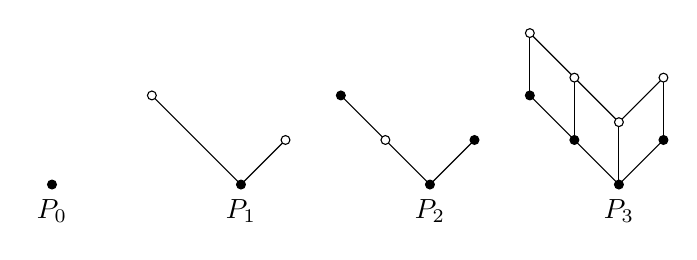
\begin{tikzpicture}[scale=0.8]
  \begin{scope}[rotate=45]
    \filldraw (0,0) circle (2pt);
    \draw (-0.3, -0.3) node {$P_0$};
  \end{scope}
  \begin{scope}[xshift=3cm,rotate=45]
    \draw (0.0, 0.0) -- (0.0, 2.0);
    \draw (0.0, 0.0) -- (1.0, 0.0);
    \filldraw[fill=black] (0.0, 0.0) circle (2pt);
    \filldraw[fill=white] (0.0, 2.0) circle (2pt);
    \filldraw[fill=white] (1.0, 0.0) circle (2pt);
    \draw (-0.3, -0.3) node {$P_1$};
  \end{scope}
  \begin{scope}[xshift=6cm,rotate=45]
    \draw (0.0, 0.0) -- (0.0, 2.0);
    \draw (0.0, 0.0) -- (1.0, 0.0);
    \filldraw[fill=black] (0.0, 0.0) circle (2pt);
    \filldraw[fill=black] (0.0, 2.0) circle (2pt);
    \filldraw[fill=black] (1.0, 0.0) circle (2pt);
    \filldraw[fill=white] (0.0, 1.0) circle (2pt);
    \draw (-0.3, -0.3) node {$P_2$};
  \end{scope}
  \begin{scope}[xshift=9cm,rotate=45]
    \draw (0.0, 2.0) -- (0.0, 0.0) -- (1.0, 0.0);
    \draw (0.7, 2.7) -- (0.7, 0.7) -- (1.7, 0.7);
    \draw (0.0, 2.0) -- (0.7, 2.7);
    \draw (0.0, 1.0) -- (0.7, 1.7);
    \draw (0.0, 0.0) -- (0.7, 0.7);
    \draw (1.0, 0.0) -- (1.7, 0.7);
    \filldraw[fill=black] (0.0, 0.0) circle (2pt);
    \filldraw[fill=black] (0.0, 2.0) circle (2pt);
    \filldraw[fill=black] (0.0, 1.0) circle (2pt);
    \filldraw[fill=black] (1.0, 0.0) circle (2pt);
    \filldraw[fill=white] (0.7, 0.7) circle (2pt);
    \filldraw[fill=white] (0.7, 2.7) circle (2pt);
    \filldraw[fill=white] (0.7, 1.7) circle (2pt);
    \filldraw[fill=white] (1.7, 0.7) circle (2pt);
    \draw (-0.3, -0.3) node {$P_3$};
  \end{scope}
\end{tikzpicture}
\end{center}
\caption{A sequence of finite posets. Each $P_n$ can be embedded into $P_{n+1}$; black nodes indicate the range of the embedding function.}
\label{fig:posets}
\end{figure}

In each step along the chain, each new poset $P_{n+1}$ is larger than the previous $P_n$ by some finite amount; the structure of $P_{n+1}$ has $P_n$ embedded within it, but it has some new elements as well.

An ep-pair between finite posets $P$ and $P'$, where $P'$ has exactly one more element than $P$, is called an \emph{increment} (terminology due to Gunter \cite{gunter92semantics}). In Fig.~\ref{fig:posets}, the embedding of $P_1$ into $P_2$ is an example of an increment.

The strategy for embedding a bifinite domain into the universal domain is built around increments. The universal domain is designed so that if a finite partial order $P$ is representable (i.e., by a deflation), and there is an increment from $P$ to $P'$, then $P'$ will also be representable.

For all embeddings from $P_n$ to $P_{n+1}$ that add more than one new value, we will need to decompose the single large embedding into a sequence of smaller increments. The challenge, then, is to determine in which order the new elements should be inserted. The order matters: Adding elements in the wrong order can cause problems, as shown in Fig.~\ref{fig:order}.

\begin{figure}
\begin{center}
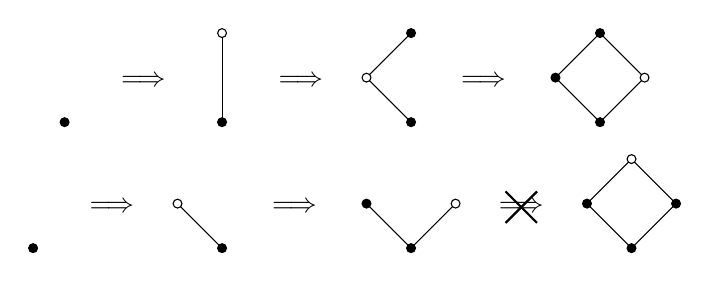
\begin{tikzpicture}[scale=0.8]
  \begin{scope}[xshift=0cm,rotate=45]
    \filldraw (0,0) circle (2pt);
  \end{scope}
  \begin{scope}[xshift=3.0cm,rotate=45]
    \draw (0.0, 0.0) -- (0.0, 1.0);
    \filldraw[fill=black] (0.0, 0.0) circle (2pt);
    \filldraw[fill=white] (0.0, 1.0) circle (2pt);
  \end{scope}
  \begin{scope}[xshift=6.0cm,rotate=45]
    \draw (0.0, 0.0) -- (0.0, 1.0);
    \draw (0.0, 0.0) -- (1.0, 0.0);
    \filldraw[fill=black] (0.0, 0.0) circle (2pt);
    \filldraw[fill=black] (0.0, 1.0) circle (2pt);
    \filldraw[fill=white] (1.0, 0.0) circle (2pt);
  \end{scope}
  \begin{scope}[xshift=9.5cm,rotate=45]
    \draw (0.0, 1.0) -- (0.0, 0.0) -- (1.0, 0.0);
    \draw (0.0, 1.0) -- (1.0, 1.0) -- (1.0, 0.0);
    \filldraw[fill=black] (0.0, 0.0) circle (2pt);
    \filldraw[fill=black] (0.0, 1.0) circle (2pt);
    \filldraw[fill=black] (1.0, 0.0) circle (2pt);
    \filldraw[fill=white] (1.0, 1.0) circle (2pt);
  \end{scope}
  \draw (1.25, 0.65) node {$\Longrightarrow$};
  \draw (4.15, 0.65) node {$\Longrightarrow$};
  \draw (7.75, 0.65) node {$\Longrightarrow$};
  \draw[thick] (7.5, 0.4) -- (8.0, 0.9);
  \draw[thick] (7.5, 0.9) -- (8.0, 0.4);

  \begin{scope}[xshift=0.5cm,yshift=2cm]
  \begin{scope}[xshift=0cm,rotate=45]
    \filldraw (0,0) circle (2pt);
  \end{scope}
  \begin{scope}[xshift=2.5cm,rotate=45]
    \draw (0.0, 0.0) -- (1.0, 1.0);
    \filldraw[fill=black] (0.0, 0.0) circle (2pt);
    \filldraw[fill=white] (1.0, 1.0) circle (2pt);
  \end{scope}
  \begin{scope}[xshift=5.5cm,rotate=45]
    \draw (0.0, 0.0) -- (0.0, 1.0) -- (1.0, 1.0);
    \filldraw[fill=black] (0.0, 0.0) circle (2pt);
    \filldraw[fill=black] (1.0, 1.0) circle (2pt);
    \filldraw[fill=white] (0.0, 1.0) circle (2pt);
  \end{scope}
  \begin{scope}[xshift=8.5cm,rotate=45]
    \draw (0.0, 0.0) -- (0.0, 1.0) -- (1.0, 1.0);
    \draw (0.0, 0.0) -- (1.0, 0.0) -- (1.0, 1.0);
    \filldraw[fill=black] (0.0, 0.0) circle (2pt);
    \filldraw[fill=black] (1.0, 1.0) circle (2pt);
    \filldraw[fill=black] (0.0, 1.0) circle (2pt);
    \filldraw[fill=white] (1.0, 0.0) circle (2pt);
  \end{scope}
  \draw (1.25, 0.65) node {$\Longrightarrow$};
  \draw (3.75, 0.65) node {$\Longrightarrow$};
  \draw (6.65, 0.65) node {$\Longrightarrow$};
  \end{scope}
\end{tikzpicture}
\end{center}
\caption{The right (top) and wrong (bottom) way to order insertions. No ep-pair exists between the 3-element and 4-element posets on the bottom row.}
\label{fig:order}
\end{figure}

To describe the position of a newly-inserted element, it will be helpful to invent some terminology. The set of elements \emph{above} the new element will be known as its \emph{superiors}. An element immediately \emph{below} the new element will be known as its \emph{subordinate}. (These terms are not in standard usage.)

In order for the insertion of a new element to be a valid increment, it must have exactly one subordinate. The subordinate indicates the value that the increment's projection maps the new value onto.

With the four-element poset in Fig.~\ref{fig:order}, it is not possible to insert the top element last. The reason is that the element has two subordinates: If a projection function maps the new element to one, the ordering relation with the other will not be preserved. Thus a monotone projection does not exist.

A strategy for successfully avoiding such situations is to always insert maximal elements first \cite[\S5]{gunter87universal}. Fig.~\ref{fig:increments} shows this strategy in action. Notice that the number of superiors varies from step to step, but each inserted element always has exactly one subordinate. To maintain this invariant, the least of the four new values must be inserted last.

\begin{figure}
\begin{center}
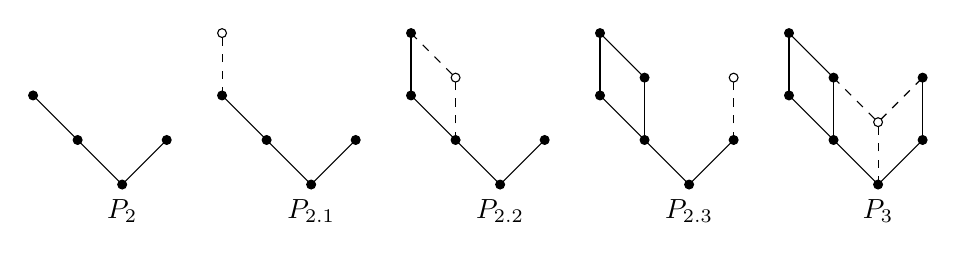
\begin{tikzpicture}[scale=0.8]
  \begin{scope}[xshift=0cm,rotate=45]
    \draw (0.0, 2.0) -- (0.0, 0.0) -- (1.0, 0.0);
    \filldraw[fill=black] (0.0, 0.0) circle (2pt);
    \filldraw[fill=black] (0.0, 2.0) circle (2pt);
    \filldraw[fill=black] (0.0, 1.0) circle (2pt);
    \filldraw[fill=black] (1.0, 0.0) circle (2pt);
    \draw (-0.3, -0.3) node {$P_2$};
  \end{scope}
  \begin{scope}[xshift=3cm,rotate=45]
    \draw (0.0, 2.0) -- (0.0, 0.0) -- (1.0, 0.0);
    \draw[dashed] (0.0, 2.0) -- (0.7, 2.7);
    \filldraw[fill=black] (0.0, 0.0) circle (2pt);
    \filldraw[fill=black] (0.0, 2.0) circle (2pt);
    \filldraw[fill=black] (0.0, 1.0) circle (2pt);
    \filldraw[fill=black] (1.0, 0.0) circle (2pt);
    \filldraw[fill=white] (0.7, 2.7) circle (2pt);
    \draw (-0.3, -0.3) node {$P_{2.1}$};
  \end{scope}
  \begin{scope}[xshift=6cm,rotate=45]
    \draw (0.0, 2.0) -- (0.0, 0.0) -- (1.0, 0.0);
    \draw (0.0, 2.0) -- (0.7, 2.7);
    \draw[dashed] (0.7, 2.7) -- (0.7, 1.7);
    \draw[dashed] (0.0, 1.0) -- (0.7, 1.7);
    \filldraw[fill=black] (0.0, 0.0) circle (2pt);
    \filldraw[fill=black] (0.0, 2.0) circle (2pt);
    \filldraw[fill=black] (0.0, 1.0) circle (2pt);
    \filldraw[fill=black] (1.0, 0.0) circle (2pt);
    \filldraw[fill=black] (0.7, 2.7) circle (2pt);
    \filldraw[fill=white] (0.7, 1.7) circle (2pt);
    \draw (-0.3, -0.3) node {$P_{2.2}$};
  \end{scope}
  \begin{scope}[xshift=9cm,rotate=45]
    \draw (0.0, 2.0) -- (0.0, 0.0) -- (1.0, 0.0);
    \draw (0.0, 2.0) -- (0.7, 2.7);
    \draw (0.7, 2.7) -- (0.7, 1.7);
    \draw (0.0, 1.0) -- (0.7, 1.7);
    \draw[dashed] (1.0, 0.0) -- (1.7, 0.7);
    \filldraw[fill=black] (0.0, 0.0) circle (2pt);
    \filldraw[fill=black] (0.0, 2.0) circle (2pt);
    \filldraw[fill=black] (0.0, 1.0) circle (2pt);
    \filldraw[fill=black] (1.0, 0.0) circle (2pt);
    \filldraw[fill=black] (0.7, 2.7) circle (2pt);
    \filldraw[fill=black] (0.7, 1.7) circle (2pt);
    \filldraw[fill=white] (1.7, 0.7) circle (2pt);
    \draw (-0.3, -0.3) node {$P_{2.3}$};
  \end{scope}
  \begin{scope}[xshift=12cm,rotate=45]
    \draw (0.0, 2.0) -- (0.0, 0.0) -- (1.0, 0.0);
    \draw (0.0, 2.0) -- (0.7, 2.7);
    \draw (0.7, 2.7) -- (0.7, 1.7);
    \draw (0.0, 1.0) -- (0.7, 1.7);
    \draw (1.0, 0.0) -- (1.7, 0.7);
    \draw[dashed] (0.7, 1.7) -- (0.7, 0.7) -- (1.7, 0.7);
    \draw[dashed] (0.0, 0.0) -- (0.7, 0.7);
    \filldraw[fill=black] (0.0, 0.0) circle (2pt);
    \filldraw[fill=black] (0.0, 2.0) circle (2pt);
    \filldraw[fill=black] (0.0, 1.0) circle (2pt);
    \filldraw[fill=black] (1.0, 0.0) circle (2pt);
    \filldraw[fill=black] (0.7, 2.7) circle (2pt);
    \filldraw[fill=black] (0.7, 1.7) circle (2pt);
    \filldraw[fill=black] (1.7, 0.7) circle (2pt);
    \filldraw[fill=white] (0.7, 0.7) circle (2pt);
    \draw (-0.3, -0.3) node {$P_3$};
  \end{scope}
\end{tikzpicture}
\end{center}
\caption{A sequence of four increments going from $P_2$ to $P_3$. Each new node may have any number of upward edges, but only one downward edge.}
\label{fig:increments}
\end{figure}

Armed with this strategy, we can finally formalize the complete sequence of increments for type $D$. To each element $x$ of the basis of $D$ we must assign a sequence number $\mathit{place}(x)$---this numbering tells in which order to insert the values. The HOLCF formalization breaks up the definition of \emph{place} as follows. First, each basis value is assigned to a rank, where $\mathit{rank}(x) = n$ means that the basis value $x$ first appears in the poset $P_n$. Equivalently, $\mathit{rank}(x)$ is the least $n$ such that $\mathit{approx}_n(x) = x$, where $\mathit{approx}_n$ is the finite deflation on $D$ with image $P_n$. Then an auxiliary function $\mathit{pos}$ assigns sequence numbers to values in finite sets, by repeatedly removing an arbitrary maximal element until the set is empty. Finally, $\mathit{place}(x)$ is defined as the sequence number of $x$ within its (finite) rank set, plus the total cardinality of all earlier ranks.
%
\begin{align}
\mathit{choose}(A) & = (\varepsilon x \in A.\ \forall y \in A.\ x \sqsubseteq y \longrightarrow x = y)
\\
pos(A,x) & =
\begin{cases} 
  0,  & \mbox{if }x = \mathit{choose}(A) \\
  1 + \mathit{pos}(A - \{\mathit{choose}(A)\}, x), & \mbox{if }x \neq \mathit{choose}(A)
\end{cases}
\\
\mathit{place}(x) & = \mathit{pos}(\{y \mid \mathit{rank}(y) = \mathit{rank}(x)\}, x) + \lVert\{y \mid \mathit{rank}(x) < \mathit{rank}(y)\}\rVert
\end{align}
For the remainder of this chapter, it will be sufficient to note that the \emph{place} function satisfies the following two properties:
%
\begin{theorem} Values in earlier ranks come before values in later ranks: If $\mathit{rank}(x) < \mathit{rank}(y)$, then $\mathit{place}(x) < \mathit{place}(y)$.
\end{theorem}
\begin{theorem} Within the same rank, larger values come first: If $\mathit{rank}(x) = \mathit{rank}(y)$ and $x \sqsubseteq y$, then $\mathit{place}(y) < \mathit{place}(x)$.
\end{theorem}

\subsection{A basis for the universal domain}
\label{sec:universal-basis}

Constructing a partial order incrementally, there are two possibilities for any newly inserted value:
%
\begin{itemize}
\item The value is the very first one (i.e., it is $\bot$)
\item The value is inserted above some previous value (its subordinate), and below zero or more other previous values (its superiors)
\end{itemize}
%
Accordingly, we can define a recursive datatype $B$ to describe the position of these values relative to each other.
%
\begin{equation}
B \mathrel{\mathop:}= \bot \mid \langle i, a, S\rangle, \mbox{where $i \in \mathbb{N}$, $a \in B$, and $S \in \mathcal{P}_f(B)$}
\end{equation}
%
The notation $\langle i, a, S\rangle$ indicates the value with serial number $i$, subordinate $a$, and the finite set of superiors $S$. (The serial number allows us to distinguish between subsequent values inserted in similar positions.)

The above definition of $B$ does not work as a datatype definition in Isabelle{\slash}HOL, because the finite set type constructor does not work with the datatype package. (Indirect recursion only works with other inductive datatypes.)  But it turns out that we do not need the datatype package at all---the type $B$ is actually isomorphic to the natural numbers. Using the bijections $\mathbb{N} \cong 1 + \mathbb{N}$ and $\mathbb{N} \cong \mathbb{N} \times \mathbb{N}$ with $\mathbb{N} \cong \mathcal{P}_f(\mathbb{N})$, we can construct a bijection that lets us use $\mathbb{N}$ as the basis datatype:
%
\begin{equation}
\mathbb{N} \cong
  1 + \mathbb{N} \times \mathbb{N} \times \mathcal{P}_f(\mathbb{N})
\end{equation}

\begin{figure}
\begin{singlespace}
\begin{center}
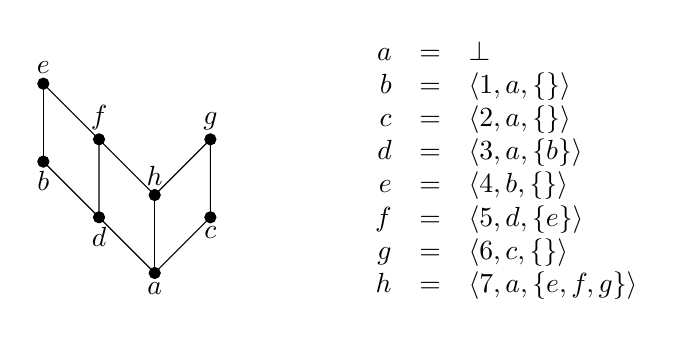
\begin{tikzpicture}
  \begin{scope}[rotate=45]
    \draw (0.0, 2.0) -- (0.0, 0.0) -- (1.0, 0.0);
    \draw (0.0, 2.0) -- (0.7, 2.7);
    \draw (0.7, 2.7) -- (0.7, 1.7);
    \draw (0.0, 1.0) -- (0.7, 1.7);
    \draw (1.0, 0.0) -- (1.7, 0.7);
    \draw (0.7, 1.7) -- (0.7, 0.7) -- (1.7, 0.7);
    \draw (0.0, 0.0) -- (0.7, 0.7);
    \filldraw (0.0, 0.0) circle (2pt) node[below] {$a$};
    \filldraw (0.0, 2.0) circle (2pt) node[below] {$b$};
    \filldraw (1.0, 0.0) circle (2pt) node[below] {$c$};
    \filldraw (0.0, 1.0) circle (2pt) node[below] {$d$};
    \filldraw (0.7, 2.7) circle (2pt) node[above] {$e$};
    \filldraw (0.7, 1.7) circle (2pt) node[above] {$f$};
    \filldraw (1.7, 0.7) circle (2pt) node[above] {$g$};
    \filldraw (0.7, 0.7) circle (2pt) node[above] {$h$};
  \end{scope}
  \draw (2.5, -0.5) node[above right] {
    $\begin{array}{rcl}
    a & = & \bot \\
    b & = & \langle 1, a, \{ \} \rangle \\
    c & = & \langle 2, a, \{ \} \rangle \\
    d & = & \langle 3, a, \{b\} \rangle \\
    e & = & \langle 4, b, \{ \} \rangle \\
    f & = & \langle 5, d, \{e\} \rangle \\
    g & = & \langle 6, c, \{ \} \rangle \\
    h & = & \langle 7, a, \{e,f,g\} \rangle
    \end{array}$
  };
\end{tikzpicture}
\end{center}
\end{singlespace}
\caption{Embedding elements of $P_3$ into the universal domain basis.}
\label{fig:encoding}
\end{figure}

Figure~\ref{fig:encoding} shows how this system works for embedding all the elements from the poset $P_3$ into the basis datatype. The elements have letter names from $a$--$h$, assigned alphabetically by insertion order. In the datatype encoding of each element, the subordinate and superiors are selected from the set of previously inserted elements. Serial numbers are assigned sequentially.

The serial number is necessary to distinguish multiple values that are inserted in the same position. For example, in Fig.~\ref{fig:encoding}, elements $b$ and $c$ both have $a$ as the subordinate, and neither has any superiors. The serial number is the only way to tell such values apart.

Note that the basis datatype seems to contain some junk---some subordinate{\slash}superiors combinations are not well formed. For example, in any valid increment, all of the superiors are positioned above the subordinate. One way to take care of this requirement would be to define a well-formedness predicate for basis elements. However, it turns out that it is possible (and indeed easier) to simply ignore any invalid elements. In the set of superiors, only those values that are above the subordinate will be considered. (This will be important to keep in mind when we define the basis ordering relation.)

There is also a possibility of multiple representations for the same value. For example, in Fig.~\ref{fig:encoding} the encoding of $h$ is given as $\langle 7, a, \{e,f,g\} \rangle$, but the representation $\langle 7, a, \{f,g\} \rangle$ would work just as well (because the sets have the same upward closure). One could consider having a well-formedness requirement for the set of superiors to be upward-closed. But this turns out not to be necessary, because the extra values do not cause problems for any of the formal proofs.

\subsection{Basis ordering relation}

To perform the ideal completion, we need to define a preorder relation on the basis. The basis value $\langle i, a, S \rangle$ should fall above $a$ and below all the values in set $S$ that are above $a$. Accordingly, we define the relation ($\preceq$) as the smallest reflexive, transitive relation that satisfies the following two introduction rules:
%
\begin{align}
\label{eq:preceq-1}
a \preceq \langle i, a, S \rangle \\
\label{eq:preceq-2}
a \preceq b \wedge b \in S \Longrightarrow \langle i, a, S \rangle \preceq b
\end{align}

Note that the relation ($\preceq$) is not antisymmetric. For example, we have both $a \preceq \langle i, a, \{a\} \rangle$ and $\langle i, a, \{a\} \rangle \preceq a$. However, for ideal completion this does not matter. Basis values $a$ and $\langle i, a, \{a\} \rangle$ generate the same principal ideal, so they will be identified as elements of the universal domain.

Also note the extra hypothesis $a \preceq b$ in Eq.~(\ref{eq:preceq-2}). Because we have not banished ill-formed subordinate/superiors combinations from the basis datatype, we must explicitly consider only those elements of the set of superiors that are above the subordinate.

\subsection {Building the embedding and projection}

%In the HOLCF formalization, the embedding function \emph{emb} from $D$ to $\mathcal{U}$ is defined using continuous extension. The first step is to define \emph{emb} on basis elements, generalizing the pattern shown in Fig.~\ref{fig:encoding}. The definition below uses wellfounded recursion---all recursive calls to \emph{emb} are on previously inserted values with smaller \emph{place} numbers:
In the HOLCF formalization, the embedding function \emph{emb} from $D$ to $\mathcal{U}$ is defined using continuous extension. We start by defining \emph{emb} on basis elements, generalizing the pattern shown in Fig.~\ref{fig:encoding}. The definition below uses wellfounded recursion---all recursive calls to \emph{emb} are on values with smaller \emph{place} numbers.
%
\begin{align}
\mathit{emb}(x) & =
\begin{cases}
\bot & \mbox{if}~x = \bot \\
\langle i, a, S \rangle & \mbox{otherwise}
\end{cases} \notag \\
\mbox{where}~i & = \mathit{place}(x) \label{eq:emb} \\
a & = \mathit{emb}(\mathit{sub}(x)) \notag \\
S & = \{\mathit{emb}(y) \mid \mathit{place}(y) < \mathit{place}(x)
\wedge x \sqsubseteq y\} \notag
\end{align}
%
The subordinate value $a$ is computed using a helper function \emph{sub}, which is defined as $\mathit{sub}(x) = \mathit{approx}_{n-1}(x)$, where $n = \mathit{rank}(x)$. The ordering produced by the \emph{place} function ensures that no previously inserted value with the same rank as $x$ will be below $x$. Therefore the previously inserted value immediately below $x$ must be $\mathit{sub}(x)$, which comes from the previous rank.

In order to complete the continuous extension, it is necessary to prove that the basis embedding function is monotone. That is, we must show that for any $x$ and $y$ in the basis of $D$, $x \sqsubseteq y$ implies $\mathit{emb}(x) \preceq \mathit{emb}(y)$. The proof is by well-founded induction over the maximum of $\mathit{place}(x)$ and $\mathit{place}(y)$. There are two main cases to consider:
%
\begin{itemize}

\item Case $\mathit{place}(x) < \mathit{place}(y)$: Because $x \sqsubseteq y$, it must be the case that $\mathit{rank}(x) < \mathit{rank}(y)$. Then, using the definition of \emph{sub} it can be shown that $x \sqsubseteq \mathit{sub}(y)$; thus by the inductive hypothesis we have $\mathit{emb}(x) \preceq \mathit{emb}(\mathit{sub}(y))$. Also, from Eq.~(\ref{eq:preceq-1}) we have $\mathit{emb}(\mathit{sub}(y)) \preceq \mathit{emb}(y)$. Finally, by transitivity we have $\mathit{emb}(x) \preceq \mathit{emb}(y)$.

\item Case $\mathit{place}(y) < \mathit{place}(x)$: From the definition of \emph{sub} we have $\mathit{sub}(x) \sqsubseteq x$. By transitivity with $x \sqsubseteq y$ this implies $\mathit{sub}(x) \sqsubseteq y$; therefore by the inductive hypothesis we have $\mathit{emb}(\mathit{sub}(x)) \preceq \mathit{emb}(y)$. Also, using Eq.~(\ref{eq:emb}), we have that $\mathit{emb}(y)$ is one of the superiors of $\mathit{emb}(x)$. Ultimately, from Eq.~(\ref{eq:preceq-2}) we have $\mathit{emb}(x) \preceq \mathit{emb}(y)$.

\end{itemize}

The projection function \emph{prj} from $\mathcal{U}$ to $D$ is also defined using continuous extension. The action of \emph{prj} on basis elements is specified by the following recursive definition:
%
\begin{equation}
\mathit{prj}(a) =
\begin{cases}
\mathit{emb}^{-1}(a) & \mbox{if}~\exists x.~\mathit{emb}(x) = a \\
\mathit{prj}(\mathit{subordinate}(a)) & \mbox{otherwise}
\end{cases}
\label{eq:prj}
\end{equation}

To ensure that \emph{prj} is well-defined, there are a couple of things to check. First of all, the recursion always terminates: In the worst case, repeatedly taking the subordinate of any starting value will eventually yield $\bot$, at which point the first branch will be taken because $\mathit{emb}(\bot) = \bot$. Secondly, note that $\mathit{emb}^{-1}$ is uniquely defined, because $\mathit{emb}$ is injective. Injectivity of \emph{emb} is easy to prove, because each embedded value has a different serial number.

Just like with \emph{emb}, we also need to prove that the basis projection function \emph{prj} is monotone. That is, we must show that for any $a$ and $b$ in the basis of $\mathcal{U}$, $a \preceq b$ implies $\mathit{prj}(a) \sqsubseteq \mathit{prj}(b)$. Remember that the basis preorder ($\preceq$) is an inductively defined relation; accordingly, the proof proceeds by induction on $a \preceq b$. Compared to the proof of monotonicity for \emph{emb}, the proof for \emph{prj} is relatively straightforward; details are omitted here.

Finally, we must prove that \emph{emb} and \emph{prj} form an ep-pair. The proof of $\mathit{prj} \circ \mathit{emb} = \mathrm{Id}_D$ is easy: Let $x$ be any value in the basis of $D$. Then using Eq.~(\ref{eq:prj}), we have $\mathit{prj}(\mathit{emb}(x)) = \mathit{emb}^{-1}(\mathit{emb}(x)) = x$. Because this equation is an admissible predicate on $x$, proving it for compact $x$ is sufficient to show that it holds for all values in the ideal completion.

The proof of $\mathit{emb} \circ \mathit{prj} \sqsubseteq \mathrm{Id}_U$ takes a bit more work. As a lemma, we can show that for any $a$ in the basis of $\mathcal{U}$, $\mathit{prj}(a)$ is always equal to $\mathit{emb}^{-1}(b)$ for some $b \preceq a$ that is in the range of \emph{emb}. Using this lemma, we then have $\mathit{emb}(\mathit{prj}(a)) = \mathit{emb}(\mathit{emb}^{-1}(b)) = b \preceq a$. Finally, using admissibility, this is sufficient to show that $\mathit{emb}(\mathit{prj}(a)) \sqsubseteq a$ for all $a$ in $\mathcal{U}$.

\subsection{Bifiniteness of the universal domain}

To show that the universal domain $\mathcal{U}$ is bifinite, we must construct a chain of finite deflations on $\mathcal{U}$ whose least upper bound is the identity function. Like all other functions in the universal domain library, these are defined by continuous extension. The action of $\mathit{uapprox}_n$ on basis elements is defined using exactly the same form of recursion as $\mathit{prj}$: We repeatedly take the subordinate of the input value, until the value satisfies some stopping criterion. With $\mathit{prj}$, the criterion was membership in the image of $\mathit{emb}$; for $\mathit{uapprox}_n$, the criterion is that the input, considered as a natural number, is less than or equal to $n$.
%
\begin{equation}
\mathit{uapprox}_n(a) =
\begin{cases}
a & \mbox{if}~a \le n \\
\mathit{uapprox}_n(\mathit{subordinate}(a)) & \mbox{otherwise}
\end{cases}
\label{eq:universal-uapprox}
\end{equation}
%
It is straightforward to show that $\mathit{uapprox}_n$ is a deflation, using induction over basis elements. Furthermore, we can show that the image of each $\mathit{uapprox}_n$ equals the set of basis elements corresponding to natural numbers $\{0..n\}$, which is a finite set. To see that $\bigsqcup_n \mathit{uapprox}_n$ is the identity function, consider that for any basis value $a$, there exists $n$ such that $\mathit{uapprox}_n(a) = a$ (namely, $n = a$).

\subsection{Implementation in HOLCF}

The universal domain type $\mathcal{U}$ is formalized in \HOLCF{11} as the type \isa{udom}. It is defined by ideal completion over the natural numbers, using the method described in Chapter~\ref{ch:powerdomain}. The complete formal proof scripts can be found in the theory file \texttt{HOLCF/Universal.thy} of the Isabelle 2011 distribution.

Most of the theory leading up to the $\mathit{emb}$ and $\mathit{prj}$ functions is parameterized by the chain $\mathit{approx}_n$ of finite deflations, using a copy of the \isa{approx_chain} locale (see Sec.~\ref{sec:pd-bifinite}).
%
\indexdef{approx_chain}
\indexthm{chain_approx}
\indexthm{lub_approx}
\indexthm{finite_deflation_approx}
\begin{isacode}
locale approx_chain =
  fixes approx :: "nat \<Rightarrow> 'a \<rightarrow> 'a"
  assumes chain_approx: "chain (\<lambda>i. approx i)"
  assumes lub_approx: "(\<Squnion>i. approx i) = ID"
  assumes finite_deflation_approx: "\<And>i. finite_deflation (approx i)"
\end{isacode}
%
The HOLCF versions of the functions $\mathit{choose}$, $\mathit{pos}$, $\mathit{rank}$, $\mathit{place}$, $\mathit{sub}$, $\mathit{emb}$ and $\mathit{prj}$ are all defined within this locale. To generate type-specific $\mathit{emb}$ and $\mathit{prj}$ functions, we could then perform locale interpretations (see Sec.~\ref{sec:pd-completion-formalize}) for specific approx-chains. However, locale interpretations would be rather wasteful: Each one would unnecessarily create copies of every constant and lemma used in the entire construction, when we really only need two constants ($\mathit{emb}$ and $\mathit{prj}$) and one lemma (stating that they form an ep-pair). As a more lightweight alternative, we define \isa{udom_emb} and \isa{udom_prj} as the parameterized versions of $\mathit{emb}$ and $\mathit{prj}$ exported from the locale.

\section{Algebraic deflations}
\label{sec:universal-alg-defl}

For solving the domain equations that arise in recursive datatype definitions, we need a cpo $\mathcal{T}$ whose values will represent bifinite domains. For this purpose, we use the set of \emph{algebraic} \emph{deflations} over the universal domain $\mathcal{U}$: We say that a deflation is algebraic if its image set is an algebraic cpo. In \HOLCF{11}, the algebraic deflations are defined using ideal completion from the set of \emph{finite} \emph{deflations}, which have finite image sets. Note that as an ideal completion, $\mathcal{T}$ is itself a cpo; this is important because it lets us use a fixed point combinator to define recursive values of type $\mathcal{T}$, representing recursive types.

\subsection{Limitations of ordinary deflations}
\label{sec:definitional-alg-limitations}

In an earlier HOLCF formalization of representable types and type constructors \cite{huffman05axiomatic}, datatypes were represented using a type of all deflations over a given cpo:
%
\begin{isacode}
pcpodef 'a deflation = "{f::'a -> 'a. deflation f}"
\end{isacode}
%
This definition yields a pointed cpo, because the \isa{deflation} predicate is admissible, and holds for \isa{\<bottom>}. As a pointed cpo, the \isa{deflation} type supports a fixed point combinator, which allows us to define recursive deflations to represent recursive datatypes. Furthermore, being defined with the \textsc{Cpodef} package makes it easy to define deflation combinators: We can use the \isa{Rep_deflation} and \isa{Abs_deflation} functions, which \textsc{Cpodef} has proved to be continuous.

\begin{isacode}
definition prod_deflation ::
    "udom deflation -> udom deflation -> udom deflation"
  where "prod_deflation = (\<Lambda> a b. Abs_deflation
    (prod_emb oo prod_map\<cdot>(Rep_deflation a)\<cdot>(Rep_deflation b) oo prod_prj))"
\end{isacode}

In the earlier formalization \cite{huffman05axiomatic}, we defined a class \isa{rep} of representable domains: These are pointed cpos that can be embedded, via an embedding-projection pair, into the universal domain.

\begin{isacode}
class rep = pcpo +
  fixes emb :: "'a -> udom"
  fixes prj :: "udom -> 'a''
  assumes ep_pair_emb_prj: "ep_pair emb prj"
\end{isacode}
%
We can obtain the representation of any type in class \isa{rep} as a value of type \isa{udom deflation}, by composing \isa{emb} and \isa{prj}. (The argument type \isa{'a itself} is pre-defined in Isabelle for use in definitions like this, where the right-hand side mentions a type variable \isa{'a}, but no actual values of type \isa{'a}. It has a single value, written \isa{TYPE('a)}.)
%
\begin{isacode}
definition rep :: "('a::rep) itself \<Rightarrow> udom deflation"
  where "rep (_ :: 'a itself) =
    Abs_deflation ((emb :: 'a \<rightarrow> udom) oo (prj :: udom \<rightarrow> 'a))"
\end{isacode}

The main problem with this approach is that class \isa{rep} is not a subclass of class \isa{bifinite}: Although \isa{udom} is algebraic, this does not imply that every type representable in \isa{udom} is algebraic. This means that if we used the above definition for a class of representable domains, then we could not use such types with the powerdomain library, which requires algebraic element types. To ensure that every representable domain is bifinite, we must restrict our attention to the algebraic deflations.

%(I could describe a specific example of a deflation on a bifinite domain whose image is not bifinite.)

\subsection{Type of algebraic deflations}
\label{sec:definitional-alg-type}

As noted above, the HOLCF type of algebraic deflations is defined as an ideal completion from the set of finite deflations. The ideal completion process described in Chapter~\ref{ch:powerdomain} requires a type to use as a basis; we define the type \isa{'a fin_defl} of finite deflations over \isa{'a} for this purpose (using the \isa{open} option, as usual, to avoid defining an extra set constant). We then proceed to define the cpo \isa{'a defl} of algebraic deflations over \isa{'a}, using the same standard process used previously for powerdomains: First define a new type as the set of ideals; then after proving that it is a cpo, define a \isa{principal} function and interpret the \isa{ideal_completion} locale.
%
\indexdef{typedef 'a fin_defl}
\begin{isacode}
typedef (open) 'a fin_defl = "{d::'a -> 'a. finite_deflation d}"
\end{isacode}
\unmedskip
\indexdef{typedef 'a defl}
\begin{isacode}
typedef (open) 'a defl = "{S :: 'a fin_defl set. below.ideal S}"
\end{isacode}
\unmedskip
\indexdef{defl_principal}
\begin{isacode}
definition defl_principal :: "'a fin_defl => 'a defl"
  where "defl_principal t = Abs_defl {u. u \<sqsubseteq> t}"
\end{isacode}
\unmedskip
\begin{isacode}
interpretation defl: ideal_completion below defl_principal Rep_defl
\end{isacode}

The most common operation on deflations is to apply them as functions. For this purpose we define the \isa{cast} operator. For a deflation \isa{t} that represents a type, \isa{cast\<cdot>t} is essentially like a type cast into that type. As type \isa{'a defl} is an ideal completion, we can define \isa{cast} as the continuous extension of \isa{Rep_fin_defl}.

\indexdef{cast}
\begin{isacode}
definition cast :: "'a defl -> 'a -> 'a"
  where "cast = defl.extension (Rep_fin_defl :: 'a fin_defl => 'a -> 'a)"
\end{isacode}

We can prove a few properties about \isa{cast} using principal induction. First, that \isa{cast} always yields deflations; second, that \isa{cast} preserves ordering.
%
\indexthm{deflation_cast}
\begin{isacode}
lemma deflation_cast: "deflation (cast\<cdot>t)"
\end{isacode}
\unmedskip
\indexthm{cast_below_cast}
\begin{isacode}
lemma cast_below_cast: "cast\<cdot>t \<sqsubseteq> cast\<cdot>u \<longleftrightarrow> t \<sqsubseteq> u"
\end{isacode}
%
The proof of \isa{cast_below_cast} is similar to many of the proofs of if-and-only-if lemmas from Chapter~\ref{ch:powerdomain}: The proposition as stated is admissible in \isa{t}, but not in \isa{u}. However, after performing principal induction on \isa{t}, reasoning about compactness shows that the remaining subgoal is admissible in \isa{u}. The proof also relies on the fact that finite deflations are compact elements of the continuous function space. A direct corollary is that the \isa{cast} function is injective, which gives us a way to prove that two given algebraic deflations are equal.

\subsection{Combinators for algebraic deflations}
\label{sec:definitional-alg-combinators}

Recall the way that Haskell deflation combinators were defined above in Sec.~\ref{sec:universal-deflation}. Each deflation combinator is written as a composition involving an ep-pair and a map function. For example the combinator \hs{tFun}, which represents the function space type, is defined like this:

\begin{hscode}
tFun :: (U -> U) -> (U -> U) -> (U -> U)
tFun a b = embFun . mapFun a b . prjFun
\end{hscode}

We would like to formalize the Haskell function \hs{tFun} in HOLCF as a function \isa{cfun_defl :: udom defl \<rightarrow> udom defl \<rightarrow> udom defl}. We already know how to formalize the other Haskell functions used in the definition of \hs{tFun}: First, the map combinator \isa{cfun_map} can represent \hs{mapFun}. Then as described in Sec.~\ref{sec:universal-features}, we can use the universal domain library to define \isa{cfun_emb} and \isa{cfun_prj} as an ep-pair from \isa{udom \<rightarrow> udom} into \isa{udom}, to model \hs{embFun} and \hs{prjFun}. Our remaining task is then to define \isa{cfun_defl} so that it meets this specification:

\begin{isacode}
lemma cast_cfun_defl:
  "cast\<cdot>(cfun_defl\<cdot>a\<cdot>b) = cfun_emb oo cfun_map\<cdot>(cast\<cdot>a)\<cdot>(cast\<cdot>b) oo cfun_prj"
\end{isacode}

As \isa{cfun_defl} is a function that takes algebraic deflations as arguments, we can define it as a continuous extension. Because we will have similar definitions for several other HOLCF type constructors besides the continuous function space, we define a generic combinator \isa{defl_fun2} that takes the \isa{emb}, \isa{prj}, and \isa{map} functions as parameters.

\indexdef{defl_fun2}
\begin{isacode}
definition defl_fun2 ::
    "('c -> 'u) => ('u -> 'c) => (('a -> 'a) -> ('b -> 'b) -> ('c -> 'c))
        => 'a defl -> 'b defl -> 'u defl"
  where "defl_fun2 e p f =
    defl.extension (\<lambda>a. defl.extension (\<lambda>b. defl_principal
      (Abs_fin_defl (e oo f\<cdot>(Rep_fin_defl a)\<cdot>(Rep_fin_defl b) oo p))))"
\end{isacode}
\unmedskip
\indexdef{cfun_defl}
\begin{isacode}
definition cfun_defl :: "udom defl \<rightarrow> udom defl \<rightarrow> udom defl"
  where "cfun_defl = defl_fun2 cfun_emb cfun_prj cfun_map"
\end{isacode}

We can then prove the lemma \isa{cast_cfun_defl} as an instance of a generic lemma about \isa{defl_fun2}. The proof involves showing that the argument to \isa{Abs_fin_defl} in the definition of \isa{defl_fun2} is actually a finite deflation. In turn, this requires that the \isa{e} and \isa{p} parameters form an ep-pair, and also that the map parameter \isa{f} preserves finite deflations.

\indexthm{cast_defl_fun2}
\begin{isacode}
lemma cast_defl_fun2:
  assumes "ep_pair e p"
  assumes
    "\<And>a b. \<lbrakk>finite_deflation a; finite_deflation b\<rbrakk> \<Longrightarrow> finite_deflation (f\<cdot>a\<cdot>b)"
  shows "cast\<cdot>(defl_fun2 e p f\<cdot>A\<cdot>B) = e oo f\<cdot>(cast\<cdot>A)\<cdot>(cast\<cdot>B) oo p"
\end{isacode}

In addition to \isa{defl_fun2}, we also define a combinator \isa{defl_fun1} for use with single-argument type constructors. Using these, we define deflation combinators for all of the type constructors in HOLCF (lifting, product, strict product, strict sum, continuous function space, and all three powerdomains).

\subsection{Type class of representable domains}
\label{sec:universal-representable}

We define a \emph{representable} domain as a cpo that can be embedded (via an ep-pair) into the universal domain. Furthermore, we require that the composition of \isa{emb} and \isa{prj} must yield an \emph{algebraic} deflation on the universal domain.
%
\indexdef{class domainn} %[sic]
\begin{isacode}
class "domain" = pcpo +
  fixes emb :: "'a \<rightarrow> udom"
  fixes prj :: "udom \<rightarrow> 'a"
  fixes defl :: "'a itself \<Rightarrow> udom defl"
  assumes ep_pair_emb_prj: "ep_pair emb prj"
  assumes cast_DEFL: "cast\<cdot>(defl TYPE('a)) = emb oo prj"
\end{isacode}
%
For convenience, we also define the syntax \isa{DEFL('a)} as shorthand for \isa{defl TYPE('a)}.

Unlike the class \isa{rep} shown earlier, this definition of class \isa{"domain"} is provably a subclass of \isa{bifinite}. The proof uses lemma \isa{obtain_principal_chain} from the \isa{ideal_completion} locale of Chapter~\ref{ch:powerdomain}. Given any algebraic deflation \isa{t}, there exists a chain of finite deflations whose least upper bound is \isa{t}. This lemma is applied to obtain a chain of finite deflations whose least upper bound is \isa{DEFL('a)}. We can then compose the elements of this chain with \isa{emb} and \isa{prj} to construct an approx-chain on type \isa{'a}.

In \HOLCF{11}, class \isa{"domain"} replaces class \isa{pcpo} as the default sort: All the types most HOLCF users will typically work with must be in class \isa{"domain"}. This means that we need class instances for each of the type constructors in HOLCF. 

Recall the Haskell \hs{Rep} class instance for the function type:
%
\begin{hscode}
instance (Rep a, Rep b) => Rep (a -> b) where
  emb = embFun . mapFun prj emb
  prj = mapFun emb prj . prjFun
\end{hscode}
%
The HOLCF \isa{"domain"} class instance for the continuous function space is defined in precisely the same way.
%
\begin{isacode}
instantiation cfun :: ("domain", "domain") "domain"
begin
  definition "emb = cfun_emb oo cfun_map\<cdot>prj\<cdot>emb"
  definition "prj = cfun_map\<cdot>emb\<cdot>prj oo cfun_prj"
  definition "defl (_ :: ('a \<rightarrow> 'b) itself) = cfun_defl\<cdot>DEFL('a)\<cdot>DEFL('b)"
  instance ...
end
\end{isacode}
%
The instance proof requires us to show that \isa{emb} and \isa{prj} are an ep-pair; this is easy to show using lemmas from Fig.~\ref{fig:universal-ep-pair-lemmas} like \isa{ep_pair_comp} and \isa{ep_pair_cfun_map}. We must also show that \isa{cast\<cdot>DEFL('a \<rightarrow> 'b) = emb oo prj}, which follows without too much trouble from \isa{cast_cfun_defl} and \isa{cast_DEFL}, using the fact that \isa{cfun_map} preserves function composition. Class instantiations for the other HOLCF type constructors (lifting, product, strict product, strict sum, and powerdomains) all follow the same pattern.

For base types like \isa{unit} and \isa{'a lift}, for which we do not have corresponding deflation combinators, the class instantiations are a little different. For these types, we can explicitly construct an approx-chain \isa{a} to establish a \isa{bifinite} class instance. Then \isa{emb} and \isa{prj} can be defined directly as \isa{udom_emb a} and \isa{udom_prj a} from the universal domain library. Finally, \isa{defl} can be defined explicitly as a least upper bound of a chain of finite deflations on \isa{udom}, based on the finite deflations from the approx-chain \isa{a}.

\section{The definitional Domain package}
\label{sec:universal-package}

Equipped with formalizations of the universal domain and algebraic deflations, it is now possible to implement the \textsc{Domain} package in a completely definitional way, without generating axioms. The purpose of this section is to describe how the new definitional implementation works---how each ``axiom'' can now be derived as a theorem.

The definitional \textsc{Domain} package reuses nearly all the code from the axiomatic \textsc{Domain} package. Figure~\ref{fig:universal-schematic} contains a copy of the implementation schematic from Chapter~\ref{ch:domain}; recall that the part in the dotted lines is where the axioms are generated. The definitional \textsc{Domain} package is identical to the axiomatic one, except that it uses a drop-in replacement for this part.

% figure copied from domain.tex
\begin{figure}
\begin{center}
\begin{singlespace}
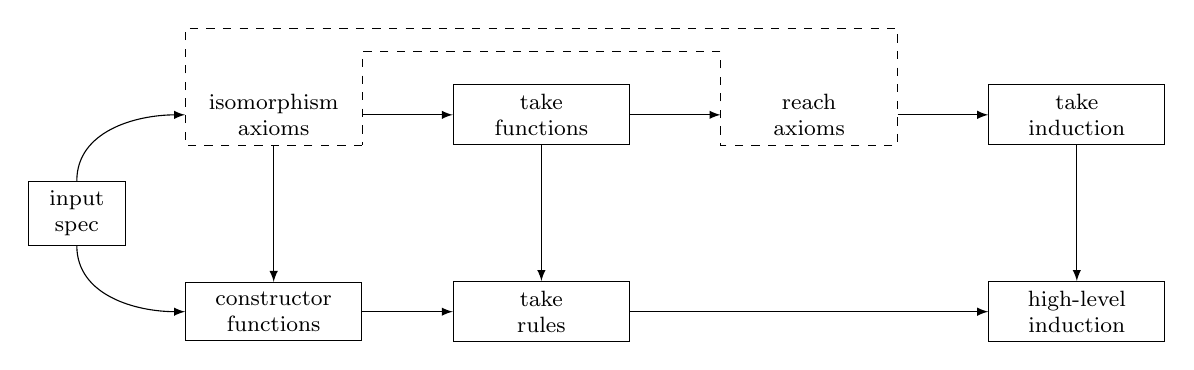
\begin{tikzpicture}
  [ axiom/.style={rectangle, text width=2cm, text centered, font=\footnotesize}
  , proof/.style={rectangle, text width=2cm, text centered, font=\footnotesize, draw}
  , >=latex]
  \node (0) at (-2.5, 1.25) [rectangle, text width=1cm, text centered, font=\footnotesize, draw] {input\\spec};
  \node (1) at (0.0, 2.5) [axiom] {isomorphism\\axioms};
  \node (2) at (3.4, 2.5) [proof] {take\\functions};
  \node (3) at (6.8, 2.5) [axiom] {reach\\axioms};
  \node (4) at (10.2, 2.5) [proof] {take\\induction};
  \node (5) at (0.0, 0.0) [proof] {constructor\\functions};
  \node (6) at (3.4, 0.0) [proof] {take\\rules};
  \node (7) at (10.2, 0.0) [proof] {high-level\\induction};
  \draw [->] (0.north) to [out=90, in=180] (1.west);
  \draw [->] (1) -- (2);
  \draw [->] (2) -- (3);
  \draw [->] (3) -- (4);
  \draw [->] (0.south) to [out=270, in=180] (5.west);
  \draw [->] (1) -- (5);
  \draw [->] (5) -- (6);
  \draw [->] (2) -- (6);
  \draw [->] (6) -- (7);
  \draw [->] (4) -- (7);
  \draw [dashed]
    (1.south east) -- (1.south west) -- (1.north west) --
    (1.west |- 0,3.6) -- (3.east |- 0,3.6) -- (3.south east) -- (3.south west) --
    (3.west |- 0,3.3) -- (1.east |- 0,3.3) -- (1.south east) -- cycle;
\end{tikzpicture}
\end{singlespace}
\end{center}
\caption{Domain package implementation schematic}
\label{fig:universal-schematic}
\end{figure}

The axiomatic \textsc{Domain} package generates two kinds of axioms: First, isomorphism axioms state that the \isa{rep} and \isa{abs} functions for each new type are each other's inverses. Second, the reach axiom for each type states a low-level induction rule, asserting that the least upper bound of a chain of take functions is the identity. The remainder of this section will show how these axioms are derived as theorems, using a lazy list datatype as an example to help explain the process.
%
\begin{isacode}
domain 'a llist = LNil | LCons (lazy "'a") (lazy "'a llist")
\end{isacode}

\subsection{Proving the isomorphism theorems}
\label{sec:universal-package-iso}

To construct a domain isomorphism for the lazy list type, information about data constructors is irrelevant; all we need is the domain equation \isa{'a llist} $\cong$ \isa{one \<oplus> ('a\<lifted> \<otimes>} \isa{'a llist\<lifted>)}. Solving this domain equation is a three-step process: The definitional \textsc{Domain} package first defines a deflation combinator, then uses the deflation to define the \isa{'a llist} type, and finally defines the isomorphism functions.

\paragraph{Defining deflation combinators.}
%
The first step is to define a deflation combinator \isa{llist_defl :: udom defl \<rightarrow> udom defl} that models the lazy list type constructor. The deflation combinator is determined by the domain equation that type \isa{'a llist} must satisfy:
%
\begin{isacode}
'a llist \<cong> one \<oplus> ('a\<lifted> \<otimes> 'a llist\<lifted>)
\end{isacode}

The definition of \isa{llist_defl} will refer to the deflation combinator of each type constructor mentioned on the right-hand side of this domain equation. To keep track of the correspondence between type constructors and deflation combinators, the \textsc{Domain} package maintains an extensible list of theorems with the \isa{[domain_defl_simps]} attribute. The initial set of these rules is shown in Fig.~\ref{fig:universal-domain-defl-simps}.

\begin{figure}
\begin{isacode}
lemma [domain_defl_simps]:
  "DEFL('a \<rightarrow> 'b) = cfun_defl\<cdot>DEFL('a)\<cdot>DEFL('b)"
  "DEFL('a \<oplus> 'b) = ssum_defl\<cdot>DEFL('a)\<cdot>DEFL('b)
  "DEFL('a \<otimes> 'b) = sprod_defl\<cdot>DEFL('a)\<cdot>DEFL('b)"
  "DEFL('a \<times> 'b) = prod_defl\<cdot>DEFL('a)\<cdot>DEFL('b)"
  "DEFL('a\<^sub>\<bottom>) = u_defl\<cdot>DEFL('a)"
  "DEFL(('a)\<sharp>) = upper_defl\<cdot>DEFL('a)"
  "DEFL(('a)\<flat>) = lower_defl\<cdot>DEFL('a)"
  "DEFL(('a)\<natural>) = convex_defl\<cdot>DEFL('a)"
\end{isacode}
\caption{Extensible set of rules with the \isa{domain_defl_simps} attribute}
\label{fig:universal-domain-defl-simps}
\end{figure}

Using \isa{domain_defl_simps}, the \textsc{Domain} package produces the recursive specification of \isa{llist_defl} shown below as \isa{llist_defl_unfold}. The actual non-recursive definition of \isa{llist_defl}, using the least fixed point combinator \isa{fix}, is created using the same machinery employed by the \textsc{Fixrec} package; \isa{llist_defl_unfold} is then derived from the non-recursive definition as a theorem.
%
\begin{isacode}
theorem llist_defl_unfold:
  "llist_defl\<cdot>t = ssum_defl\<cdot>DEFL(one)\<cdot>(sprod_defl\<cdot>(u_defl\<cdot>t)\<cdot>(u_defl\<cdot>(llist_defl\<cdot>t)))"
\end{isacode}

\paragraph{Defining representable domains from deflations.}
%
The second step is to use \isa{llist_defl} to define the actual \isa{'a llist} type. In Sections \ref{sec:definitional-alg-combinators} and \ref{sec:universal-representable}, the aim was to build algebraic deflations of type \isa{udom defl} to correspond with pre-existing cpo types. Now, we need to do the converse: Given a deflation of type \isa{udom defl}, we must define the corresponding cpo. We can accomplish this with the help of the \textsc{Cpodef} package.

The first step in defining a new cpo type with \textsc{Cpodef} is to determine a subset of values of the old cpo type. We define the \isa{defl_set} function for this purpose: It produces the image set of any deflation \isa{t}, defined as the set of fixed points of \isa{cast\<cdot>t}.
\vspace{-22pt} % FUDGE
\indexdef{defl_set}
\begin{isacode}
definition defl_set :: "'a defl \<Rightarrow> 'a set"
  where "defl_set t = {x. cast\<cdot>t\<cdot>x = x}"
\end{isacode}
%
Now we can define \isa{'a llist} as a pointed cpo, isomorphic to the image set of the deflation \isa{llist_defl\<cdot>DEFL('a)}.
%
\begin{isacode}
pcpodef (open) 'a llist = "defl_set (llist_defl\<cdot>DEFL('a))"
\end{isacode}
%
The \textsc{Cpodef} package generates two proof obligations: First, that membership in the given set is admissible, and also that the given set contains \isa{\<bottom>}. Both of these properties hold for any application of \isa{defl_set}.

\indexthm{adm_defl_set}
\begin{isacode}
lemma adm_defl_set: "adm (\<lambda>x. x \<in> defl_set t)"
\end{isacode}
\unmedskip
\indexthm{defl_set_bottom}
\begin{isacode}
lemma defl_set_bottom: "\<bottom> \<in> defl_set t"
\end{isacode}

The \isa{pcpodef} command only proves that type \isa{'a llist} is a \isa{pcpo}; we still need to provide an instantiation of the \isa{"domain"} class. This instantiation requires definitions of \isa{emb}, \isa{prj}, and \isa{defl}, which are defined as follows:
%
\begin{isacode}
instantiation llist :: ("domain") "domain"
begin
  definition "(emb :: 'a llist \<rightarrow> udom) \<equiv> (\<Lambda> x. Rep_llist x)"
  definition "(prj :: udom \<rightarrow> 'a llist) \<equiv>
      (\<Lambda> x. Abs_llist (cast\<cdot>(llist_defl\<cdot>DEFL('a))\<cdot>x))"
  definition "defl \<equiv> (\<lambda>(_ :: 'a llist itself). llist_defl\<cdot>DEFL('a))"
  instance ...
end
\end{isacode}
%
The instance proof requires us to show that \isa{emb} and \isa{prj} are an ep-pair, and also that the composition \isa{emb oo prj} is equal to \isa{cast\<cdot>DEFL('a llist)}. Instead of repeating this proof for each new domain definition, we employ a generic lemma that proves the \isa{OFCLASS} predicate, in the style of the lemmas used to implement \textsc{Cpodef}.
%
\indexthm{typedef_domain_class}
\begin{isacode}
lemma typedef_domain_class:
  fixes Rep :: "'a::pcpo \<Rightarrow> udom"
  fixes Abs :: "udom \<Rightarrow> 'a::pcpo"
  fixes t :: "udom defl"
  assumes type: "type_definition Rep Abs (defl_set t)"
  assumes below: "below \<equiv> (\<lambda>x y. Rep x \<sqsubseteq> Rep y)"
  assumes emb: "emb \<equiv> (\<Lambda> x. Rep x)"
  assumes prj: "prj \<equiv> (\<Lambda> x. Abs (cast\<cdot>t\<cdot>x))"
  assumes defl: "defl \<equiv> (\<lambda>(_ :: 'a itself). t)"
  shows "OFCLASS('a, domain_class)"
\end{isacode}
%
The assumptions \isa{type} and \isa{below} in this rule can be satisfied by theorems generated by \textsc{Cpodef}; the other assumptions are simply the definitions from the \isa{"domain"} class instantiation.

After proving the class instance, we can extend \isa{domain_defl_simps} with a new rule for the lazy list type constructor; this rule follows immediately from the definition of \isa{defl} for lazy lists.
%
\indexthmx{DEFL_llist}
\begin{isacode}
theorem DEFL_llist [domain_defl_simps]: "DEFL('a llist) = llist_defl\<cdot>DEFL('a)"
\end{isacode}

This entire process of defining a representable domain from a deflation is automated with the \textsc{Domaindef} package, which is built as a thin layer on top of the \textsc{Cpodef} package. \textsc{Domaindef} is called internally by the definitional \textsc{Domain} package, and it is also available as a user-level command. Unlike \textsc{Cpodef}, it is completely automatic; no additional proof obligations are needed.
%
\begin{isacode}
domaindef 'a llist = "llist_defl\<cdot>DEFL('a)"
\end{isacode}
%
The above \isa{domaindef} command defines type \isa{'a llist}, proves a \isa{"domain"} class instance, and adds theorem \isa{DEFL_llist} to \isa{domain_defl_simps}.

\paragraph{Constructing isomorphism functions as coercions.}

The third step is to actually construct the desired domain isomorphism, by defining continuous \isa{rep} and \isa{abs} functions and proving that they are each other's inverses.

For any representable domains \isa{'a} and \isa{'b}, composing \isa{emb :: 'a \<rightarrow> udom} with \isa{prj :: udom \<rightarrow> 'b} yields a \emph{coercion} \isa{prj oo emb :: 'a \<rightarrow> 'b}. If \isa{DEFL('a) \<sqsubseteq> DEFL('b)}, then the coercions from \isa{'a} to \isa{'b} and back form an ep-pair. If \isa{DEFL('a) = DEFL('b)}, then the coercions from \isa{'a} to \isa{'b} and back form a continuous isomorphism. The \textsc{Domain} package uses this fact to define the \isa{rep} and \isa{abs} functions for each new domain, and show that they form a continuous isomorphism.

\indexdefx{llist_rep}
\begin{isacode}
definition llist_rep :: "'a llist \<rightarrow> one \<oplus> ('a\<lifted> \<otimes> 'a llist\<lifted>)"
  where "llist_rep \<equiv> prj oo emb"
\end{isacode}
\unmedskip
\indexdefx{llist_abs}
\begin{isacode}
definition llist_abs :: "one \<oplus> ('a\<lifted> \<otimes> 'a llist\<lifted>) \<rightarrow> 'a llist"
  where "llist_abs \<equiv> prj oo emb"
\end{isacode}

Before we can prove that \isa{llist_rep} and \isa{llist_abs} are a continuous isomorphism, we must prove that the types they coerce between are represented by the same deflation. Theorem \isa{DEFL_eq_llist} is easily proved using \isa{domain_defl_simps} together with \isa{llist_defl_unfold}.
%
\indexthmx{DEFL_eq_llist}
\begin{isacode}
theorem DEFL_eq_llist: "DEFL('a llist) = DEFL(one \<oplus> ('a\<lifted> \<otimes> 'a llist\<lifted>))"
\end{isacode}

Using \isa{DEFL_eq_llist}, the definitional \textsc{Domain} package can \emph{prove} that \isa{llist_abs} and \isa{llist_rep} are an isomorphism---in the axiomatic \textsc{Domain} package, \isa{llist.abs_iso} and \isa{llist.rep_iso} would have been declared as axioms.
%
\indexthmx{llist.abs_iso}
\begin{isacode}
theorem llist.abs_iso: "llist_rep\<cdot>(llist_abs\<cdot>x) = x"
\end{isacode}
\unmedskip
\indexthmx{llist.rep_iso}
\begin{isacode}
theorem llist.rep_iso: "llist_abs\<cdot>(llist_rep\<cdot>y) = y"
\end{isacode}
%
Theorem \isa{llist.abs_iso} is proved by instantiating lemma \isa{domain_abs_iso} from the library with \isa{DEFL_eq_llist} and the definitions of \isa{llist_abs} and \isa{llist_rep}.
%
\indexthm{domain_abs_iso}
\begin{isacode}
lemma domain_abs_iso:
  fixes abs :: "'a \<rightarrow> 'b" and rep :: "'b \<rightarrow> 'a"
  assumes DEFL: "DEFL('b) = DEFL('a)"
  assumes abs_def: "abs \<equiv> prj oo emb"
  assumes rep_def: "rep \<equiv> prj oo emb"
  shows "rep\<cdot>(abs\<cdot>x) = x"
\end{isacode}
%
Theorem \isa{llist_rep_iso} is proved using a similar rule, \isa{domain_rep_iso}, which concludes \isa{abs\<cdot>(rep\<cdot>y) = y} from the same assumptions.

\subsection{Proving the reach lemma}
\label{sec:universal-package-reach}

After the new definitional \textsc{Domain} package code constructs the isomorphism, the take-function component (described in Chapter~\ref{ch:domain}) defines \isa{llist_take}, and proves some theorems (listed in Fig.~\ref{fig:universal-llist-take}). Now the definitional \textsc{Domain} package needs to prove the reach lemma, which states that the least upper bound of the chain \isa{llist_take} is the identity function.

\begin{figure}
\begin{isacode}
theorem llist.take_def:
  "llist_take \<equiv> (\<lambda>n. iterate n\<cdot>
    (\<Lambda> g. llist_abs oo ssum_map\<cdot>ID\<cdot>(sprod_map\<cdot>ID\<cdot>(u_map\<cdot>g)) oo llist_rep)\<cdot>\<bottom>)"
\end{isacode}
\unmedskip
\begin{isacode}
theorem llist.take_0: "llist_take 0 = \<bottom>"
\end{isacode}
\unmedskip
\begin{isacode}
theorem llist.take_Suc: "llist_take (Suc n) =
  llist_abs oo ssum_map\<cdot>ID\<cdot>(sprod_map\<cdot>ID\<cdot>(u_map\<cdot>(llist_take n))) oo llist_rep"
\end{isacode}
\unmedskip
\begin{isacode}
theorem llist.chain_take: "chain llist_take"
\end{isacode}
\unmedskip
\begin{isacode}
theorem llist.deflation_take: "deflation (llist_take n)"
\end{isacode}
\caption{Definition and basic properties of \isa{llist_take} function}
\label{fig:universal-llist-take}
\end{figure}

As an integrated part of the process of deriving the reach lemma, the definitional \textsc{Domain} package also performs the necessary steps to allow indirect recursion with \isa{llist} in later domain definitions. This involves defining a map function \isa{llist_map}, proving a few theorems about it, and adding those theorems to the appropriate databases.

The overall process can be broken down into three main steps: First, define the map function. Second, prove the identity law for the map function, by establishing a relationship between the map function and the deflation combinator. Third, prove the reach lemma by relating the take function to the map function.

\paragraph{Defining the map function.}

The \textsc{Domain} package defines the map function \isa{llist_map} of type \isa{('a \<rightarrow> 'a) \<rightarrow> 'a llist \<rightarrow> 'a llist}.\footnote{The most general type of \isa{llist_map} is actually \isa{('a \\<rightarrow> 'b) \\<rightarrow> 'a llist \\<rightarrow> 'b llist}. However, the current implementation uses the more restrictive type scheme because it works without modification for contravariant types. Generalizing the types of map functions is planned as future work.} It generates a recursive specification from a combination of other map functions, based on the structure of the type \isa{one \<oplus> ('a\<lifted> \<otimes> 'a llist\<lifted>)}. As with the deflation combinator, the actual fixed point definition is handled by \textsc{Fixrec}-style machinery.
%
\begin{isacode}
theorem llist_map_unfold:
  "llist_map\<cdot>f = llist_abs oo
    ssum_map\<cdot>ID\<cdot>(sprod_map\<cdot>(u_map\<cdot>f)\<cdot>(u_map\<cdot>(llist_map\<cdot>f))) oo llist_rep"
\end{isacode}

At this point the \textsc{Domain} package proves one of the rules needed for later indirect-recursive definitions, which states that \isa{llist_map} preserves deflations. Theorem \isa{deflation_llist_map} is proved by fixed point induction, using the pre-existing \isa{domain_deflation} rules; it is then added to the \isa{domain_deflation} rule database.
%
\begin{isacode}
theorem deflation_llist_map [domain_deflation]:
  "deflation f \<Longrightarrow> deflation (llist_map\<cdot>f)"
\end{isacode}

\paragraph{Proving the identity law.}

The other property that we must prove about \isa{llist_map} is the identity law, \isa{llist_map\<cdot>ID = ID}. To prove this property, the \textsc{Domain} package exploits the similarities in the recursive definitions of \isa{llist_map} and the \isa{llist_defl}. The relationship between the two is formalized in a binary relation called \isa{isodefl}, which states that the given function \isa{f} is ``isomorphic'' in some sense to the algebraic deflation \isa{t}.

\begin{isacode}
definition isodefl :: "('a::domain \<rightarrow> 'a) \<Rightarrow> udom defl \<Rightarrow> bool"
  where "isodefl f t = (cast\<cdot>t = emb oo f oo prj)"
\end{isacode}

The \textsc{Domain} package maintains a database of theorems relating map functions to their corresponding deflation combinators, using the attribute \isa{[domain_isodefl]}. The initial contents of this database are shown in Fig.~\ref{fig:universal-domain-isodefl}.

\begin{figure}
\begin{isacode}
lemma [domain_isodefl]:
  "isodefl (ID :: 'a \<rightarrow> 'a) DEFL('a)"
  "\<lbrakk>isodefl f1 t1; isodefl f2 t2\<rbrakk> \<Longrightarrow> isodefl (cfun_map\<cdot>f1\<cdot>f2) (cfun_defl\<cdot>t1\<cdot>t2)"
  "\<lbrakk>isodefl f1 t1; isodefl f2 t2\<rbrakk> \<Longrightarrow> isodefl (ssum_map\<cdot>f1\<cdot>f2) (ssum_defl\<cdot>t1\<cdot>t2)"
  "\<lbrakk>isodefl f1 t1; isodefl f2 t2\<rbrakk> \<Longrightarrow> isodefl (sprod_map\<cdot>f1\<cdot>f2) (sprod_defl\<cdot>t1\<cdot>t2)"
  "\<lbrakk>isodefl f1 t1; isodefl f2 t2\<rbrakk> \<Longrightarrow> isodefl (prod_map\<cdot>f1\<cdot>f2) (prod_defl\<cdot>t1\<cdot>t2)"
  "isodefl f t \<Longrightarrow> isodefl (u_map\<cdot>f) (u_defl\<cdot>t)"
  "isodefl f t \<Longrightarrow> isodefl (upper_map\<cdot>f) (upper_defl\<cdot>t)"
  "isodefl f t \<Longrightarrow> isodefl (lower_map\<cdot>f) (lower_defl\<cdot>t)"
  "isodefl f t \<Longrightarrow> isodefl (convex_map\<cdot>f) (convex_defl\<cdot>t)"
\end{isacode}
\caption{Extensible set of rules with the \isa{domain_isodefl} attribute}
\label{fig:universal-domain-isodefl}
\end{figure}

Now the \textsc{Domain} package must prove a similar \isa{domain_isodefl} rule for the lazy list type:
%
\begin{isacode}
theorem isodefl_llist [domain_isodefl]:
  "isodefl f t \<Longrightarrow> isodefl (llist_map\<cdot>f) (llist_defl\<cdot>t)"
\end{isacode}
%
The proof proceeds by a form of parallel fixed point induction: After unfolding the definitions of \isa{llist_map} and \isa{llist_defl} to reveal the underlying fixed point combinators, rule \isa{parallel_fix_ind} can be applied.
%
\begin{isacode}
lemma parallel_fix_ind:
  "\<lbrakk>adm (\<lambda>x. P (fst x) (snd x)); P \<bottom> \<bottom>; \<And>x y. P x y \<Longrightarrow> P (F\<cdot>x) (G\<cdot>y)\<rbrakk>
    \<Longrightarrow> P (fix\<cdot>F) (fix\<cdot>G)"
\end{isacode}
%
After discharging the admissibility check and the base case \isa{isodefl \<bottom> \<bottom>}, the final subgoal is nontrivial:

\begin{isacode}
goal (1 subgoal):
 1. \<And>x y. \<lbrakk>isodefl f t; isodefl x y\<rbrakk>
\end{isacode}
\pagebreak
\begin{isacode}
          \<Longrightarrow> isodefl
              (llist_abs oo
               ssum_map\<cdot>ID\<cdot>(sprod_map\<cdot>(u_map\<cdot>f)\<cdot>(u_map\<cdot>x)) oo llist_rep)
              (ssum_defl\<cdot>DEFL(one)\<cdot>(sprod_defl\<cdot>(u_defl\<cdot>t)\<cdot>(u_defl\<cdot>y)))
\end{isacode}
%
This last subgoal is solved by repeatedly applying rules from the \isa{domain_isodefl} database, along with one extra rule to handle the occurrences of \isa{llist_abs} and \isa{llist_rep}:
%
\begin{isacode}
theorem llist.isodefl_abs_rep:
  "isodefl f t \<Longrightarrow> isodefl (llist_abs oo f oo llist_rep) t"
\end{isacode}
%
A similar theorem holds for any \isa{rep} and \isa{abs} functions defined as coercions between isomorphic types.

Once theorem \isa{isodefl_llist} has been proven, the \textsc{Domain} package uses lemmas \isa{isodefl_DEFL_imp_ID} and \isa{DEFL_llist} to derive the identity law for \isa{llist_map} as a corollary.
%
\indexthm{isodefl_DEFL_imp_ID}
\begin{isacode}
lemma isodefl_DEFL_imp_ID: "isodefl f DEFL('a) \<Longrightarrow> f = ID"
\end{isacode}
\unmedskip
\indexthmx{llist_map_ID}
\begin{isacode}
theorem llist_map_ID [domain_map_ID]: "llist_map\<cdot>ID = ID"
\end{isacode}
%
Once proved, \isa{llist_map_ID} is added to the \isa{domain_map_ID} database (introduced in Chapter~\ref{ch:domain}) for use in later domain definitions.

\paragraph{Relating the map and take functions.}

In the final step, the reach lemma can be derived from the identity law of \isa{llist_map}, by taking advantage of similarities in the definitions of \isa{llist_take} and \isa{llist_map}.
%
\begin{isacode}
theorem llist.lub_take: "(\<Squnion>n. llist_take n) = ID"
\end{isacode}
%
The proof begins by applying transitivity with \isa{llist_map_ID}, yielding the subgoal 
\isa{(\<Squnion>n. llist_take n)} \isa{= llist_map\<cdot>ID}. After unfolding the definitions of \isa{llist_take}, \isa{llist_map}, and the fixed point combinator \isa{fix}, both sides of the equality have the form \isa{(\<Squnion>n. iterate\<cdot>f\<cdot>\<bottom>)}. Rewriting with \isa{domain_map_ID} rules can finish the proof.

\subsection{User-visible changes}

In \HOLCF{11}, the \textsc{Domain} package operates in definitional mode by default. For backward compatibility, the axiomatic mode is still available using the \isa{domain} \isa{(unsafe)} command. The primary user-visible difference between the two modes is which type classes they use: In definitional mode, type parameters and other constructor argument types must be in class \isa{"domain"}; newly-defined datatypes are also made instances of the \isa{"domain"} class. In contrast, the axiomatic mode uses the \isa{pcpo} class throughout. Even with this change, most HOLCF user theories work without modification, because the default sort has also changed from \isa{pcpo} to \isa{"domain"}.

The other user-visible change is the new support for indirect recursion. After defining type \isa{'a llist} with the definitional \textsc{Domain} package, users can define other datatypes using indirect recursion with \isa{llist}, such as this datatype of trees:
%
\begin{isacode}
domain 'a tree = Leaf (lazy "'a") | Node (lazy "'a tree llist")
\end{isacode}
%
In axiomatic mode, however, the \textsc{Domain} package does not generate map functions, and does not configure indirect recursion to work with new datatypes.

\section{Unpointed predomains}
\label{sec:universal-predomain}

Prior to \HOLCF{11}, \isa{pcpo} has always been the default sort; any type variables mentioned in HOLCF theories were assumed to be in class \isa{pcpo} by default. However, the class \isa{cpo}, which is a superclass of \isa{pcpo} that does not require a bottom element, is also useful in some cases. Various theory developments based on \HOLCF{99} have made use of the \isa{cpo} class \cite{hol+lcf, mueller98thesis}. With \HOLCF{11} switching from \isa{pcpo} to the \isa{"domain"} class, what should be done with these theories that use class \isa{cpo}? There is a need for an unpointed variant of class \isa{"domain"} in \HOLCF{11}.

To fill this need, we introduce a class of \emph{predomains}. A predomain is a cpo that, when lifted, becomes a representable domain. More precisely, while \isa{'a::"domain"} means that type \isa{'a} can be embedded into \isa{udom}, \isa{'a::predomain} means that type \isa{'a\<^sub>\<bottom>} can be embedded into \isa{udom\<^sub>\<bottom>}.

\indexdef{class predomain_syn}
\begin{isacode}
class predomain_syn = cpo +
  fixes liftemb :: "'a\<^sub>\<bottom> \<rightarrow> udom\<^sub>\<bottom>"
  fixes liftprj :: "udom\<^sub>\<bottom> \<rightarrow> 'a\<^sub>\<bottom>"
  fixes liftdefl :: "'a itself \<Rightarrow> (udom\<^sub>\<bottom>) defl"
\end{isacode}
\unmedskip
\indexdef{class predomain}
\begin{isacode}
class predomain = predomain_syn +
  assumes predomain_ep: "ep_pair liftemb liftprj"
  assumes cast_liftdefl: "cast\<cdot>(liftdefl TYPE('a)) = liftemb oo liftprj"
\end{isacode}
%
We also define \isa{LIFTDEFL('a)} as a convenient abbreviation for \isa{liftdefl TYPE('a)}.

Shortly we will redefine the \isa{"domain"} type class to make it into a subclass of \isa{predomain}. But in order to do that, we need a function for creating deflations on \isa{udom\<^sub>\<bottom>} out of deflations on \isa{udom}.

\indexdef{liftdefl_of}
\begin{isacode}
definition liftdefl_of :: "udom defl \<rightarrow> (udom\<^sub>\<bottom>) defl"
  where "liftdefl_of = defl_fun1 ID ID u_map"
\end{isacode}
\unmedskip
\indexthm{cast_liftdefl_of}
\begin{isacode}
lemma cast_liftdefl_of: "cast\<cdot>(liftdefl_of\<cdot>t) = u_map\<cdot>(cast\<cdot>t)"
\end{isacode}
%
We now extend the \isa{"domain"} type class by adding \isa{predomain_syn} as a superclass, along with a few class assumptions stating that \isa{liftemb}, \isa{liftprj}, and \isa{liftdefl} are defined in a standard way.
%
\begin{isacode}
class "domain" = predomain_syn + pcpo +
  fixes emb :: "'a \<rightarrow> udom"
  fixes prj :: "udom \<rightarrow> 'a"
  fixes defl :: "'a itself \<Rightarrow> udom defl"
  assumes ep_pair_emb_prj: "ep_pair emb prj"
  assumes cast_DEFL: "cast\<cdot>(defl TYPE('a)) = emb oo prj"
  assumes liftemb_eq: "liftemb = u_map\<cdot>emb"
  assumes liftprj_eq: "liftprj = u_map\<cdot>prj"
  assumes liftdefl_eq: "liftdefl TYPE('a) = liftdefl_of\<cdot>(defl TYPE('a))"
\end{isacode}
%
It is then a simple matter to prove the subclass relationship \isa{"domain" \<subseteq> predomain}, by showing that the definitions of \isa{liftemb}, \isa{liftprj}, and \isa{liftdefl} specified by the \isa{"domain"} class satisfy the \isa{predomain} axioms.

\paragraph{Domain class instance for lifted cpo.} Now we define a new \isa{"domain"} class instance for the lifted cpo type \isa{'a\<^sub>\<bottom>}, so that the type argument \isa{'a} only needs to be a \isa{predomain}. To implement this class instance, we need a new variant of the deflation combinator \isa{u_defl} whose argument type is \isa{(udom\<^sub>\<bottom>) defl} instead of \isa{udom defl}.
%
\indexdef{u_liftdefl}
\begin{isacode}
definition u_liftdefl :: "(udom\<^sub>\<bottom>) defl \<rightarrow> udom defl"
  where "u_liftdefl = defl_fun1 u_emb u_prj ID"
\end{isacode}
\unmedskip
\indexthm{cast_u_liftdefl}
\begin{isacode}
lemma cast_u_liftdefl: "cast\<cdot>(u_liftdefl\<cdot>t) = u_emb oo cast\<cdot>t oo u_prj"
\end{isacode}
%
Here \isa{u_emb :: udom\<^sub>\<bottom> \<rightarrow> udom} and \isa{u_prj :: udom \<rightarrow> udom\<^sub>\<bottom>} are the ep-pair provided by the universal domain library---the same functions are used to define \isa{u_defl}. The two deflation combinators are related by the following theorem:
%
\indexthm{u_liftdefl_liftdefl_of}
\begin{isacode}
lemma u_liftdefl_liftdefl_of: "u_liftdefl\<cdot>(liftdefl_of\<cdot>t) = u_defl\<cdot>t"
\end{isacode}
%
This means that although \isa{DEFL('a\<^sub>\<bottom>) = u_liftdefl\<cdot>LIFTDEFL('a)} by definition, it is also still equal to \isa{u_defl\<cdot>DEFL('a)} for any \isa{'a} in class \isa{"domain"}, just as it was defined before.
%
\begin{isacode}
instantiation u :: (predomain) "domain"
begin
  definition "(emb :: 'a\<^sub>\<bottom> \<rightarrow> udom) = u_emb oo liftemb"
  definition "(prj :: udom \<rightarrow> 'a\<^sub>\<bottom>) = liftprj oo u_prj"
  definition "defl (_ :: ('a\<^sub>\<bottom>) itself) = u_liftdefl\<cdot>LIFTDEFL('a)"
  ...
end
\end{isacode}
%
The functions \isa{liftemb}, \isa{liftprj}, and \isa{liftdefl} are all defined exactly as required by the \isa{"domain"} class axioms. The other \isa{"domain"} class axioms about \isa{emb}, \isa{prj}, and \isa{defl} follow from the \isa{predomain} class axioms on type \isa{'a}.

\paragraph{Predomain class instance for cartesian product.}

The goal here is to create a \isa{predomain} instance for products, such that the product of two predomains is again a predomain. To do this, we must create an ep-pair from type \isa{('a \<times> 'b)\<^sub>\<bottom>} into \isa{udom\<^sub>\<bottom>}. To define the embedding and projection, we make use of an isomorphism between type \isa{('a \<times> 'b)\<^sub>\<bottom>} and the strict product \isa{'a\<^sub>\<bottom> \<otimes> 'b\<^sub>\<bottom>}.

\indexdef{encode_prod_u}
\begin{isacode}
definition encode_prod_u :: "('a \<times> 'b)\<^sub>\<bottom> \<rightarrow> 'a\<^sub>\<bottom> \<otimes> 'b\<^sub>\<bottom>"
  where "encode_prod_u = (\<Lambda>(up\<cdot>(x, y)). (:up\<cdot>x, up\<cdot>y:))"
\end{isacode}
\unmedskip
\indexdef{decode_prod_u}
\begin{isacode}
definition decode_prod_u :: "'a\<^sub>\<bottom> \<otimes> 'b\<^sub>\<bottom> \<rightarrow> ('a \<times> 'b)\<^sub>\<bottom>"
  where "decode_prod_u = (\<Lambda>(:up\<cdot>x, up\<cdot>y:). up\<cdot>(x, y))"
\end{isacode}

The embedding can now be done in multiple steps: Starting with a value of type \isa{('a \<times> 'b)\<^sub>\<bottom>}, first apply \isa{encode_prod_u} to get a strict pair of type \isa{'a\<^sub>\<bottom> \<otimes> 'b\<^sub>\<bottom>}. Second, map \isa{liftemb} over each component of the strict pair to get another pair of type \isa{udom\<^sub>\<bottom> \<otimes> udom\<^sub>\<bottom>}. Third, apply \isa{decode_prod_u} to convert this to type \isa{(udom \<times> udom)\<^sub>\<bottom>}. Finally, map the embedding function for type \isa{udom \<times> udom} over the lifted cpo to get a value of type \isa{udom\<^sub>\<bottom>}. The projection uses the same process in reverse. We then define the deflation combinator \isa{prod_liftdefl} to correspond with the composition of these embedding and projection functions.

\indexdef{prod_liftdefl}
\begin{isacode}
definition prod_liftdefl :: "(udom\<^sub>\<bottom>) defl \<rightarrow> (udom\<^sub>\<bottom>) defl \<rightarrow> (udom\<^sub>\<bottom>) defl"
  where "prod_liftdefl = defl_fun2 (u_map\<cdot>prod_emb oo decode_prod_u)
    (encode_prod_u oo u_map\<cdot>prod_prj) sprod_map"
\end{isacode}
\unmedskip
\indexthm{cast_prod_liftdefl}
\begin{isacode}
lemma cast_prod_liftdefl:
  "cast\<cdot>(prod_liftdefl\<cdot>a\<cdot>b) = (u_map\<cdot>prod_emb oo decode_prod_u) oo
    sprod_map\<cdot>(cast\<cdot>a)\<cdot>(cast\<cdot>b) oo (encode_prod_u oo u_map\<cdot>prod_prj)"
\end{isacode}
\unmedskip
\begin{isacode}
instantiation prod :: (predomain, predomain) predomain
begin
  definition "liftemb = (u_map\<cdot>prod_emb oo decode_prod_u)
      oo (sprod_map\<cdot>liftemb\<cdot>liftemb oo encode_prod_u)"
  definition "liftprj = (decode_prod_u oo sprod_map\<cdot>liftprj\<cdot>liftprj)
      oo (encode_prod_u oo u_map\<cdot>prod_prj)"
  definition "liftdefl (_ :: ('a \<times> 'b) itself) =
      prod_liftdefl\<cdot>LIFTDEFL('a)\<cdot>LIFTDEFL('b)"
  instance ...
end
\end{isacode}
%
Although the definitions may look complex, the \isa{predomain} instance proof is still relatively simple. Showing \isa{ep_pair liftemb liftprj} merely requires a few extra applications of rules from Fig.~\ref{fig:universal-ep-pair-lemmas}.
%
\begin{isacode}
instantiation prod :: ("domain", "domain") "domain"
begin
  definition "(emb :: 'a \<times> 'b \<rightarrow> udom) = prod_emb oo prod_map\<cdot>emb\<cdot>emb"
  definition "(prj :: udom \<rightarrow> 'a \<times> 'b) = prod_map\<cdot>prj\<cdot>prj oo prod_prj"
  definition "defl (_ :: ('a \<times> 'b) itself) = prod_defl\<cdot>DEFL('a)\<cdot>DEFL('b)"
  instance ...
end
\end{isacode}
%
On the other hand, the \isa{"domain"} instance proof requires more work than one might expect. The reason is that unlike any other \isa{"domain"} class instantiation, the product type does not have \isa{liftemb}, \isa{liftprj}, and \isa{liftdefl} defined exactly as specified by the \isa{"domain"} class axioms. Fortunately, \isa{liftemb = u_map\<cdot>emb} and \isa{liftprj = u_map\<cdot>prj} can be proved without too much trouble by case analysis on their inputs. Also, \isa{LIFTDEFL('a \<times> 'b) = liftdefl_of\<cdot>DEFL('a \<times> 'b)} can be proved using the injectivity of \isa{cast}, by showing that \isa{cast\<cdot>LIFTDEFL('a \<times> 'b) = cast\<cdot>(liftdefl_of\<cdot>DEFL('a \<times> 'b))}.

\paragraph{Other class instances.} Other \isa{predomain} class instances can be defined in a similar way to the product type. For example, with the Isabelle/HOL disjoint sum type, an isomorphism can be defined between type \isa{('a + 'b)\<^sub>\<bottom>} and the strict sum \isa{'a\<^sub>\<bottom> \<oplus> 'b\<^sub>\<bottom>}. This can be used to show that the disjoint sum of two predomains is again a predomain.

Another isomorphism that was noted back in Chapter~\ref{ch:holcf} is between type \isa{'a discr\<^sub>\<bottom>} and \isa{'a lift}. This is used to make \isa{'a discr} an instance of class \isa{predomain}, for any countable type \isa{'a}.

The last new class instance of note is for the continuous function type. To show that type \isa{'a \<rightarrow> 'b} is in class \isa{pcpo}, \isa{'b} must be a \isa{pcpo}, but \isa{'a} only needs to be in class \isa{cpo}. How can we get a similar instance for the \isa{"domain"}  and \isa{predomain} classes? In order to prove this class instance, we can define a type \isa{'a \<rightarrow>! 'b}, which is the \emph{strict function space} from \isa{'a} to \isa{'b}.
%
\begin{isacode}
pcpodef (open) ('a, 'b) sfun (infixr "\<rightarrow>!" 0) = "{f :: 'a \<rightarrow> 'b. f\<cdot>\<bottom> = \<bottom>}"
\end{isacode}
%
For an unpointed \isa{'a} and pointed \isa{'b}, type \isa{'a \<rightarrow> 'b} is isomorphic to the strict function type \isa{'a\<^sub>\<bottom> \<rightarrow>! 'b}. This can then be used to obtain the desired class instance for continuous functions.

\paragraph{Domain package support for predomains.} Some minor changes to the \textsc{Domain} package were necessary to add support for predomains. Two new features were implemented. First, lazy constructor arguments are now permitted to be in class \isa{predomain}. (Strict constructor arguments are still required to be in class \isa{"domain"}.) For example, we can define the following type of lazy lists of natural numbers, where the elements have the unpointed type \isa{nat discr}:
%
\begin{isacode}
domain natlist = nil | cons (lazy "nat discr") (lazy "natlist")
\end{isacode}
%
The second feature is that datatypes can now have type parameters in class \isa{predomain}. For example, we can define a variation of the lazy list datatype that allows unpointed predomain element types:
%
\begin{isacode}
domain ('a::predomain) ulist = unil | ucons (lazy "'a") (lazy "'a ulist")
\end{isacode}
%
Note that the constructor argument \isa{'a} is lazy, as it must be for the definition to be accepted.

To support these new features, the part of the \textsc{Domain} package that defines deflation combinators had to be updated. For domains with unpointed type parameters, the type of the deflation combinator is different: For example, \isa{llist_defl} had type \isa{udom defl \<rightarrow> udom defl}, while \isa{ulist_defl} has type \isa{(udom\<^sub>\<bottom>) defl \<rightarrow> udom defl}. Because the \isa{domain_defl_simps} rules are used to generate deflation combinator definitions, we must also declare a few more rules with this attribute (Fig.~\ref{fig:universal-predomain-defl-simps}).

\begin{isacode}
theorem ulist_defl_unfold: "ulist_defl\<cdot>t =
  ssum_defl\<cdot>DEFL(one)\<cdot>(sprod_defl\<cdot>(u_liftdefl\<cdot>t)\<cdot>(u_defl\<cdot>(ulist_defl\<cdot>t)))"
\end{isacode}

\begin{figure}
\begin{isacode}
lemma [domain_defl_simps]:
  "DEFL('a\<^sub>\<bottom>) = u_liftdefl\<cdot>LIFTDEFL('a)"
  "LIFTDEFL('a::"domain") = liftdefl_of\<cdot>DEFL('a)"
  "u_liftdefl\<cdot>(liftdefl_of\<cdot>t) = u_defl\<cdot>t"
  "LIFTDEFL('a \<times> 'b) = prod_liftdefl\<cdot>LIFTDEFL('a)\<cdot>LIFTDEFL('b)"
  "DEFL(('a::predomain) \<rightarrow> 'b) = DEFL('a\<^sub>\<bottom> \<rightarrow>! 'b)"
\end{isacode}
\caption{Additional \isa{domain_defl_simps} rules for predomains}
\label{fig:universal-predomain-defl-simps}
\end{figure}

The \textsc{Domaindef} package also needs modification to handle the changed definition of the \isa{"domain"} class. Lemma \isa{typedef_domain_class} gets three extra assumptions, corresponding to the class axioms \isa{liftemb_eq}, \isa{liftprj_eq}, and \isa{liftdefl_eq}; \textsc{Domaindef} defines these constants accordingly for each instance.

For the proofs of the identity law for map functions, we must define a variant of the \isa{isodefl} relation for use with the \isa{predomain} class. We also extend the initial set of \isa{domain_isodefl} rules with a few new ones about \isa{isodefl'}, shown in Fig.~\ref{fig:universal-predomain-isodefl}.
%
\begin{isacode}
definition isodefl' :: "('a::predomain \<rightarrow> 'a) \<Rightarrow> (udom\<^sub>\<bottom>) defl \<Rightarrow> bool"
  where "isodefl' f t \<longleftrightarrow> cast\<cdot>t = liftemb oo u_map\<cdot>f oo liftprj"
\end{isacode}

\begin{figure}
\begin{isacode}
lemma [domain_isodefl]:
  "isodefl' (ID :: 'a \<rightarrow> 'a) LIFTDEFL('a::predomain)"
  "isodefl f t \<Longrightarrow> isodefl' f (liftdefl_of\<cdot>t)"
  "isodefl' f t \<Longrightarrow> isodefl (u_map\<cdot>f) (u_liftdefl\<cdot>t)"
  "\<lbrakk>isodefl' f1 t1; isodefl' f2 t2\<rbrakk> \<Longrightarrow> isodefl' (prod_map\<cdot>f1\<cdot>f2) (prod_liftdefl\<cdot>t1\<cdot>t2)"
\end{isacode}
\caption{Additional \isa{domain_isodefl} rules for predomains}
\label{fig:universal-predomain-isodefl}
\end{figure}

The \isa{domain_isodefl} rules for new domains must mention this variant if they have any predomain type parameters. For example, consider the \isa{'a ulist} type:
\pagebreak
\begin{isacode}
theorem isodefl_ulist [domain_isodefl]:
  "isodefl' f t \<Longrightarrow> isodefl (ulist_map\<cdot>f) (ulist_defl\<cdot>t)"
\end{isacode}

Perhaps surprisingly, these few changes listed here are the only ones necessary to support the new predomain features. All of the other proof scripts in the rest of the \textsc{Domain} package continue to work without modification in the presence of predomains.

\section{Related work and conclusion}
\label{sec:universal-conclusion}

An early example of the purely definitional approach to defining datatypes is described by Melham, in the context of the HOL theorem prover \cite{melham89automating}. Melham defines a type $(\alpha)\mathit{Tree}$ of labelled trees, from which other recursive types are defined as subsets. The design is similar in spirit to the one presented in this chapter---types are modeled as values, and abstract properties that characterize each datatype are proved as theorems. The main differences are that Melham uses ordinary types instead of bifinite domains, and ordinary subsets instead of deflations.

The Isabelle/HOL datatype package uses a design very similar to the HOL system. The type $\alpha~\mathit{node}$, which was originally used for defining recursive types in Isabelle/HOL, was introduced by Paulson \cite{paulson97mechanizing}; it is quite similar to the HOL system's $(\alpha)\mathit{Tree}$ type. E. Gunter later extended the labelled tree type of HOL to support datatypes with arbitrary branching \cite{gunter94broader}. Berghofer and Wenzel used a similarly extended type to implement the current version of Isabelle's datatype package \cite{bw99inductivedatatypes}.

Agerholm used a variation of Melham's labelled trees to define lazy lists and other recursive domains in the HOL-CPO system \cite{agerholm94thesis}. Agerholm's cpo of infinite trees can represent arbitrary polynomial datatypes as subsets; however, negative recursion is not supported.

Recent work by Benton, et al.\ uses the colimit construction to define recursive domains in Coq \cite{bkv2009coq}. Like the universal domain described in this chapter, their technique can handle both positive and negative recursion. Using colimits avoids the need for a universal domain, but it requires a logic with dependent types; the construction will not work in ordinary higher-order logic.

On the theoretical side, various publications by C. Gunter \cite{gunter85thesis, gunter87universal, gunter92semantics} were the primary sources of ideas for the HOLCF universal domain construction. The construction of the sequence of increments in Section~\ref{sec:universal-construction} is just as described by Gunter \cite[\S5]{gunter87universal}. However, the use of ideal completion is original---Gunter defines the universal domain using a colimit construction instead. Given a cpo $D$, Gunter defines a type $D^+$ that can embed any increment from $D$ to $D'$. The universal domain is then defined as a solution to the domain equation $D = D^+$. The construction of $D^+$ is similar to our basis datatype $B$, except that it is non-recursive and does not include serial numbers.

Another universal domain with similar features has been described by D. Scott \cite{gunter90semantic, Scott08}. The domain \textsf{U} is defined by ideal completion, where the basis is a countable free boolean algebra minus its top element. It is proved to be a universal domain for the class of \emph{bounded complete} algebraic cpos (also commonly known as \emph{Scott domains}) which is a subclass of the bifinite cpos. Compared to the universal bifinite domain \isa{udom}, its basis has a much simpler definition, and would have been significantly easier to formalize; however, bounded completeness is not preserved by the convex powerdomain.

While the literature only claims that the domain \textsf{U} can represent bounded complete cpos, it is actually possible that it could represent arbitrary \emph{bifinite} cpos as well. The construction described in this chapter is based on encoding increments of posets, where the new element $\langle i, a, S \rangle$ with serial number $i$ is inserted above the element $a$ and below each element in the finite set $S$. In the free boolean algebra with generators $(x_i)_{i\in\omega}$, we could encode the value $\langle i, a, S \rangle$ as $(x_i \sqcap a) \sqcup (\neg x_i \sqcap (\bigsqcap S))$. As long as each inserted value uses a distinct serial number, this encoding appears to satisfy the appropriate ordering relations. Exploring this idea in more detail is reserved for future work.

Earlier versions of portions of this chapter have been published previously \cite{huffman09universal}. The formalization of the universal domain in \HOLCF{11} differs sightly from that earlier presentation in its treatment of the chain of \isa{approx} functions: Previously, \isa{approx} was an overloaded function of the \isa{bifinite} type class, and \isa{udom_emb} and \isa{udom_prj} were polymorphic functions in the same type class. In contrast, the new version uses a locale to fix the chain of \isa{approx} functions.

In summary, the \HOLCF{11} universal domain library provides the basic infrastructure upon which the new \textsc{Domain} package can construct general recursive datatypes in a purely definitional way. It provides a type \isa{udom}, along with the means to construct an ep-pair into \isa{udom} from any other bifinite cpo. Such ep-pairs are a prerequisite for building deflation combinators that represent type constructors. In turn, the \textsc{Domain} package now uses deflation combinators to define recursive datatypes, proving the type isomorphism and induction rules without generating axioms.

\chapter{Case Study and Conclusion: Verifying Monads}
\label{ch:case-domain}

\section{Introduction}

The primary claim of this thesis is that \HOLCF{11} offers a superior environment for program verification---specifically, we claim that \HOLCF{11} provides an unprecented combination of \emph{expressiveness}, \emph{automation}, and \emph{confidence}.
Expressiveness means that users can accurately and concisely specify the datatypes, functions, and properties that they want to reason about. The new and improved definition packages in \HOLCF{11} make it easy to translate a wider variety of recursive datatype and function definitions than ever before. Automation means that users can avoid expending effort on trivial proof details, and focus on the interesting parts of more difficult proofs. Theorems that are straightforward to prove on paper (and also some that are not so easy on paper) have almost completely automatic proofs in \HOLCF{11}. The new proof automation also helps users to prove large, complex theorems with minimal effort. Confidence means that there is a strong argument for believing in the correctness of the system---\HOLCF{11} provides confidence by adhering to a purely definitional approach, and avoiding new axioms.

The goal of this chapter is to provide evidence for these claims. The level of confidence has already been established in the previous chapters, which describe the purely definitional implementation of \HOLCF{11}. To measure the expressiveness and automation available in \HOLCF{11}, we consider case studies where we prove properties about specific functional programs. Finally, to support the claim that the combination of these qualities in \HOLCF{11} is \emph{unprecedented}, we compare \HOLCF{11} with some earlier approaches to program verification, evaluating them along the axes of expressiveness, automation, and confidence.

For the case studies in this chapter, we examine some monad types of the kind often used in Haskell programming. Recall that monads are typically used to implement computations with side-effects, such as exceptions or mutable state---different monad types provide different kinds of side-effects. Every monad is equipped with a \emph{return} operation, which returns a value without side-effects; and a \emph{bind} operation, which sequences computations by feeding the result of one computation into the next. These operations are expected to satisfy a set of monad laws. Also, individual monads may have other operations that are expected to satisfy additional laws. For example, a mutable-state monad would have \emph{read} and \emph{write} operations that should satisfy some simple properties.

The example monads used in this chapter range from simple to complex: First we have the basic type of lazy lists, which is ubiquitous in Haskell programming. Later on we consider a much more complex monad with multiple kinds of side-effects, that is useful for modeling concurrency. Its definition is built up from simpler monads in stages, using \emph{monad transformers} \cite{Moggi89, LHJ95}. The definitions and proofs for lazy lists serve primarily to show how well \HOLCF{11} handles easy verification tasks, while the concurrency monad is intended to test the full extent of \HOLCF{11}'s capabilities.

In addition to verifying the monad laws for each type, we also define and verify some other type-specific operations. For lazy lists, we formalize the Haskell functions \hs{repeat}, which generates infinite lists; and \hs{zipWith}, which applies a function pointwise to two lists. For the concurrency monad, we formalize an operation that nondeterministically interleaves two computations. Each of these operations satisfies a set of laws that comes from the theory of \emph{applicative functors} \cite{McBride08}.

\paragraph{Contributions.} The case studies here primarily serve to demonstrate the tools described in the earlier chapters, but they introduce some new technical contributions as well. Some new proof techniques have been developed to help automate some of the proofs presented in this chapter:
%
\begin{itemize*}
\item Parallel fixed point induction using depth parameters (\S\ref{sec:case-coinductive})
\item Principle of \emph{map-induction} for indirect-recursive datatypes (\S\ref{sec:case-induct-R})
\end{itemize*}

\paragraph{Overview.} The remainder of this chapter is organized as follows: Section~\ref{sec:case-lazy-list} covers the lazy list monad case study. After defining the datatype and list operations (\S\ref{sec:case-llist-definition}), we verify the monad laws (\S\ref{sec:case-llist-monad}). Next we consider the applicative functor instance with \hs{repeat} and \hs{zipWith} (\S\ref{sec:case-applicative}) and their correctness proofs (\S\ref{sec:case-verify-applicative}). One law in particular requires more advanced coinductive proof techniques; we evaluate some standard methods, and compare them with a new technique using induction over depth parameters (\S\ref{sec:case-coinductive}).

Section~\ref{sec:case-concurrency-monad} discusses the development of the concurrency monad. The concurrency monad is built up using a sequence of standard monads and monad transformers (\S\ref{sec:case-composing-monads}--\ref{sec:case-resumption-transformer}), ultimately being defined by the \textsc{Domain} package (\S\ref{sec:case-define-R}). After developing the \emph{map-induction} principle for reasoning about the concurrency monad (\S\ref{sec:case-induct-R}), we verify the monad operations (\S\ref{sec:case-verify-R}) and the nondeterministic interleaving operator (\S\ref{sec:case-zipR}).

Section~\ref{sec:case-related} contains a survey of related work, where we compare the attributes of \HOLCF{11} with those of various earlier systems and approaches to program verification. Finally, Sec.~\ref{sec:case-conclusion} gives a summary and some closing remarks.

\section{The lazy list monad}
\label{sec:case-lazy-list}

In this section, we formalize a lazy list type in HOLCF, which models the standard Haskell list type. We also define the functor and monad operations on the lazy list type, corresponding to the standard Haskell definitions of \hs{fmap}, \hs{return} and \hs{(>{}>=)} for lists, and prove the standard laws about them. The definitions and laws for the functor and monad classes are shown in Figs.~\ref{fig:case-functor-laws} and \ref{fig:case-monad-laws}; the class instances for lists are given in Fig.~\ref{fig:case-list-instances}.

\begin{figure}
\begin{center}
\begin{minipage}{0.90\textwidth}
\begin{hscode}
class Functor f where
  fmap :: (a -> b) -> f a -> f b
\end{hscode}
\begin{hscode}
        fmap id v = v               -- Identity
fmap g (fmap h v) = fmap (g . h) v  -- Composition
\end{hscode}
\end{minipage}
\end{center}
\caption{Haskell class \texttt{Functor}, with functor laws}
\label{fig:case-functor-laws}
\end{figure}

\begin{figure}
\begin{center}
\begin{minipage}{0.90\textwidth}
\begin{hscode}
class Monad m where
  return :: a -> m a
  (>>=) :: m a -> (a -> m b) -> m b
\end{hscode}
\begin{hscode}
 (return x >>= g) = g x                        -- Left unit
   (v >>= return) = v                          -- Right unit
((v >>= g) >>= h) = (v >>= (\x -> g x >>= h))  -- Associativity
\end{hscode}
\end{minipage}
\end{center}
\caption{Haskell class \texttt{Monad}, with monad laws}
\label{fig:case-monad-laws}
\end{figure}

\begin{figure}
\begin{center}
\begin{minipage}{0.80\textwidth}
\begin{hscode}
data [a] = [] | a : [a]
\end{hscode}
\begin{hscode}
instance Functor [] where
  fmap g [] = []
  fmap g (x : xs) = g x : fmap g xs
\end{hscode}
\begin{hscode}
(++) :: [a] -> [a] -> [a]
[]       ++ ys = ys
(x : xs) ++ ys = x : (xs ++ ys)
\end{hscode}
\begin{hscode}
instance Monad [] where
  return x = [x]
  []       >>= k = []
  (x : xs) >>= k = k x ++ (xs >>= k)
\end{hscode}
\end{minipage}
\end{center}
\caption{Haskell \texttt{Functor} and \texttt{Monad} instances for lazy lists}
\label{fig:case-list-instances}
\end{figure}

\HOLCF{11} aims to make easy proofs automatic, and hard proofs possible. These properties of Haskell list operations are examples of easy proofs---the goal of this section is to illustrate how simple it is to formalize the definitions in HOLCF, and how easy and automated the proofs can be.

\subsection{Datatype and function definitions}
\label{sec:case-llist-definition}

The first step in formalizing the Haskell list monad in HOLCF is to define the type using the \textsc{Domain} package. We use the name \isa{llist} for lazy lists in HOLCF, to avoid a clash with the existing Isabelle/HOL \isa{list} datatype.
%
\indexdefx{domain 'a llist}
\begin{isacode}
domain 'a llist = LNil | LCons (lazy "'a") (lazy "'a llist")
\end{isacode}
%
Among the many theorems generated by this call to the \textsc{Domain} package, one of the most important is \isa{llist.induct}: It is used in every proof that involves induction over lazy lists.
%
\indexthmx{llist.induct}
\begin{isacode}
theorem llist.induct:
  "\<lbrakk>adm P; P \<bottom>; P LNil; \<And>x xs. P xs \<Longrightarrow> P (LCons\<cdot>x\<cdot>xs)\<rbrakk> \<Longrightarrow> P ys"
\end{isacode}

We formalize the Haskell list functions \hs{fmap}, \hs{return}, \hs{(++)}, and \hs{(>{}>=)} in HOLCF as \isa{mapL}, \isa{unitL}, \isa{appendL}, and \isa{bindL}, respectively (see Fig.~\ref{fig:case-list-holcf}). Each of them is defined using \textsc{Fixrec}, except for \isa{unitL}; because \isa{unitL} does not need pattern matching or recursion, a simple \isa{definition} suffices. In addition to the defining equations, we also generate strictness rules for each function. Each strictness rule is proved by a single application of the \isa{fixrec_simp} method (introduced in Chapter~\ref{ch:fixrec}).

\begin{figure}
\indexdefx{mapL}
\begin{isacode}
fixrec mapL :: "('a \<rightarrow> 'b) \<rightarrow> 'a llist \<rightarrow> 'b llist"
  where "mapL\<cdot>f\<cdot>LNil = LNil"
  | "mapL\<cdot>f\<cdot>(LCons\<cdot>x\<cdot>xs) = LCons\<cdot>(f\<cdot>x)\<cdot>(mapL\<cdot>f\<cdot>xs)"
\end{isacode}
\unmedskip
\indexdefx{unitL}
\begin{isacode}
definition unitL :: "'a \<rightarrow> 'a llist"
  where "unitL = (\<Lambda> x. LCons\<cdot>x\<cdot>LNil)"
\end{isacode}
\unmedskip
\indexdefx{appendL}
\begin{isacode}
fixrec appendL :: "'a llist \<rightarrow> 'a llist \<rightarrow> 'a llist"
  where "appendL\<cdot>LNil\<cdot>ys = ys"
  | "appendL\<cdot>(LCons\<cdot>x\<cdot>xs)\<cdot>ys = LCons\<cdot>x\<cdot>(appendL\<cdot>xs\<cdot>ys)"
\end{isacode}
\unmedskip
\indexdefx{bindL}
\begin{isacode}
fixrec bindL :: "'a llist \<rightarrow> ('a \<rightarrow> 'b llist) \<rightarrow> 'b llist"
  where "bindL\<cdot>LNil\<cdot>f = LNil"
  | "bindL\<cdot>(LCons\<cdot>x\<cdot>xs)\<cdot>f = appendL\<cdot>(f\<cdot>x)\<cdot>(bindL\<cdot>xs\<cdot>f)"
\end{isacode}
\unmedskip
\indexthmx{mapL_strict}
\begin{isacode}
lemma mapL_strict [simp]: "mapL\<cdot>f\<cdot>\<bottom> = \<bottom>"
  by fixrec_simp
\end{isacode}
\unmedskip
\indexthmx{appendL_strict}
\begin{isacode}
lemma appendL_strict [simp]: "appendL\<cdot>\<bottom>\<cdot>ys = \<bottom>"
  by fixrec_simp
\end{isacode}
\unmedskip
\indexthmx{bindL_strict}
\begin{isacode}
lemma bindL_strict [simp]: "bindL\<cdot>\<bottom>\<cdot>f = \<bottom>"
  by fixrec_simp
\end{isacode}
\caption{HOLCF formalization of functor and monad operations for lazy lists}
\label{fig:case-list-holcf}
\end{figure}

\subsection{Verifying the functor and monad laws}
\label{sec:case-llist-monad}

With all the operations defined and the rewrite rules added to the simplifier, we can proceed to prove the functor and monad laws. The proofs of both functor laws for lazy lists are completely automatic: Just apply induction followed by simplification.
%
\indexthmx{mapL_ID}
\begin{isacode}
lemma mapL_ID: "mapL\<cdot>ID\<cdot>xs = xs"
  by (induct xs, simp_all)
\end{isacode}
\unmedskip
\indexthmx{mapL_mapL}
\begin{isacode}
lemma mapL_mapL: "mapL\<cdot>f\<cdot>(mapL\<cdot>g\<cdot>xs) = mapL\<cdot>(f oo g)\<cdot>xs"
  by (induct xs, simp_all)
\end{isacode}
%
The right unit law for the lazy list monad has a similar automatic proof, as long as we tell the simplifier to unfold the definition of \isa{unitL}.

\indexthmx{bindL_unitL_right}
\begin{isacode}
lemma bindL_unitL_right: "bindL\<cdot>xs\<cdot>unitL = xs"
  by (induct xs, simp_all add: unitL_def)
\end{isacode}

The proofs of the other two monad laws are slightly more difficult. While they still have a high level of automation, each proof requires one or more lemmas. We will consider the left unit law first.

The left unit law for the lazy list monad requires that \isa{bindL\<cdot>(unitL\<cdot>x)\<cdot>g = g\<cdot>x}. If we unfold the definition of \isa{unitL} and simplify, we are left with the subgoal \isa{appendL\<cdot>(g\<cdot>x)\<cdot>LNil = g\<cdot>x}. To proceed, we must back up and prove a lemma saying that appending \isa{LNil} on the right leaves a list unchanged. With the help of lemma \isa{appendL_LNil_right}, the left unit law can then be proved automatically.
 %
\indexthmx{appendL_LNil_right}
\begin{isacode}
lemma appendL_LNil_right: "appendL\<cdot>xs\<cdot>LNil = xs"
  by (induct xs, simp_all)
\end{isacode}
\unmedskip
\indexthmx{bindL_unitL}
\begin{isacode}
lemma bindL_unitL: "bindL\<cdot>(unitL\<cdot>x)\<cdot>g = g\<cdot>x"
  by (simp add: unitL_def appendL_LNil_right)
\end{isacode}

Finally we consider the associativity law, which asserts that \isa{bindL\<cdot>(bindL\<cdot>xs\<cdot>g)\<cdot>h} \isa{=} \isa{bindL\<cdot>xs\<cdot>(\<Lambda> x. bindL\<cdot>(g\<cdot>x)\<cdot>h)}. If we perform induction on \isa{xs}, the simplifier can automatically solve all subgoals but one: In the \isa{LCons} case, the left hand side \isa{bindL\<cdot>(bindL\<cdot>(LCons\<cdot>x\<cdot>xs)\<cdot>g)\<cdot>h} reduces to 
\isa{bindL\<cdot>(appendL\<cdot>(g\<cdot>x)\<cdot>(bindL\<cdot>xs\<cdot>g))\<cdot>h}, but then we get stuck: We need to prove a lemma to show that \isa{bindL} distributes over \isa{appendL}.

We can try to prove \isa{bindL\<cdot>(appendL\<cdot>xs\<cdot>ys)\<cdot>g = appendL\<cdot>(bindL\<cdot>xs\<cdot>g)\<cdot>(bindL\<cdot>ys\<cdot>g)} as a lemma, by induction on \isa{xs}. As before, simplification discharges everything but the \isa{LCons\<cdot>x\<cdot>xs} case: After simplifying and rewriting with the inductive hypothesis, the left-hand side reduces to \isa{appendL\<cdot>(g\<cdot>x)\<cdot>(appendL\<cdot>(bindL\<cdot>xs\<cdot>g)\<cdot>(bindL\<cdot>ys\<cdot>g))}. The right-hand side is similar, but has the appends grouped the other way: \isa{appendL\<cdot>} \isa{(appendL\<cdot>(g\<cdot>x)\<cdot>(bindL\<cdot>xs\<cdot>g))\<cdot>(bindL\<cdot>ys\<cdot>g)}. This suggests yet another lemma: We must prove that \isa{appendL} is associative.

At last, the associativity of \isa{appendL} can be proved directly by induction on \isa{xs}, without needing any more lemmas. After \isa{appendL_appendL}, we can now give fully automatic proofs for \isa{bindL_appendL} and \isa{bindL_bindL}, where each theorem uses the previous one as a rewrite rule.
%
\indexthmx{appendL_appendL}
\begin{isacode}
lemma appendL_appendL:
    "appendL\<cdot>(appendL\<cdot>xs\<cdot>ys)\<cdot>zs = appendL\<cdot>xs\<cdot>(appendL\<cdot>ys\<cdot>zs)"
  by (induct xs, simp_all)
\end{isacode}
\unmedskip
\indexthmx{bindL_appendL}
\begin{isacode}
lemma bindL_appendL:
    "bindL\<cdot>(appendL\<cdot>xs\<cdot>ys)\<cdot>g = appendL\<cdot>(bindL\<cdot>xs\<cdot>g)\<cdot>(bindL\<cdot>ys\<cdot>g)"
  by (induct xs, simp_all add: appendL_appendL)
\end{isacode}
\unmedskip
\indexthmx{bindL_bindL}
\begin{isacode}
lemma bindL_bindL: "bindL\<cdot>(bindL\<cdot>xs\<cdot>g)\<cdot>h = bindL\<cdot>xs\<cdot>(\<Lambda> x. bindL\<cdot>(g\<cdot>x)\<cdot>h)"
  by (induct xs, simp_all add: bindL_appendL)
\end{isacode}

\subsection{Applicative functors and laws for zip}
\label{sec:case-applicative}

The functor and monad operations, \hs{fmap}, \hs{return} and \hs{(>{}>=)}, are not the only functions on lazy lists with standard algebraic laws that we ought to verify. The \emph{applicative functors} are another algebraic class of which lazy lists can be made an instance. The particular instance discussed here is based on the standard Haskell functions \hs{repeat} and \hs{zipWith}; in this section we prove that these operations satisfy the appropriate \emph{applicative functor laws}.

The class of applicative functors for Haskell was introduced recently by McBride and Paterson \cite{McBride08}. An applicative functor is more than a functor, but less than a monad: Applicative functors support sequencing of effects, but not binding. The class is defined in Haskell as shown in Fig.~\ref{fig:case-applicative-laws}. It fixes two functions: First, \hs{pure} lifts an ordinary value into the applicative functor type; it denotes a computation with no effects, much like \hs{return} for monads. Second, the left-associative infix operator \hs{(<*>)} takes two computations, respectively yielding a function and an argument, and applies them together, sequencing their effects. All reasonable implementations of \hs{pure} and \hs{(<*>)} are expected to satisfy the four laws listed in Fig.~\ref{fig:case-applicative-laws}.\footnote{In the composition law, \hs{(.) :: (b -> c) -> (a -> b) -> a -> c} denotes function composition.}

\begin{figure}
\begin{hscode}
class Applicative f where
  pure :: a -> f a
  (<*>) :: f (a -> b) -> f a -> f b   -- left-associative
\end{hscode}
\begin{hscode}
             pure id <*> v = v                      -- Identity
pure (.) <*> u <*> v <*> w = u <*> (v <*> w)        -- Composition
         pure g <*> pure x = pure (g x)             -- Homomorphism
              u <*> pure y = pure (\g -> g y) <*> u -- Interchange
\end{hscode}
\caption{Haskell class \texttt{Applicative}, with applicative functor laws}
\label{fig:case-applicative-laws}
\end{figure}

There is more than one way to instantiate class \hs{Applicative} for the lazy list type. One possibility, which works for any monad, is to define \hs{pure} and \hs{(<*>)} in terms of the monadic operations \hs{return} and \hs{(>{}>=)}, as shown below.
%
\begin{hscode}
instance Applicative [] where
  pure x = return x
  fs <*> xs = fs >>= (\f -> xs >>= (\x -> return (f x)))
\end{hscode}
%
With these definitions, the four applicative functor laws can be proven by rewriting with the monad laws. An applicative functor instance can be derived from any monad in the same way. In terms of demonstrating proof techniques in HOLCF, this instantiation is rather unpromising.

For our purposes, a different instantiation using \hs{repeat} and \hs{zipWith} offers a more interesting verification challenge for \HOLCF{11}. The full code for the applicative functor instance is shown in Fig.~\ref{fig:case-applicative-list-instance}. In this version, sequencing is done by taking a list of functions and a list of arguments, and applying them pointwise. The ``effect'' being sequenced here is essentially the dependence of values on their positions in the list. A pure computation (with no such ``effect'') is then represented as an infinite list whose elements are all the same.

\begin{figure}
\begin{center}
\begin{minipage}{0.90\textwidth}
\begin{hscode}
repeat :: a -> [a]
repeat x = x : repeat x
\end{hscode}
\begin{hscode}
zipWith :: (a -> b -> c) -> [a] -> [b] -> [c]
zipWith f (x : xs) (y : ys) = f x y : zipWith f xs ys
zipWith f _ _ = []
\end{hscode}
\begin{hscode}
instance Applicative [] where
  pure x = repeat x
  fs <*> xs = zipWith id fs xs
\end{hscode}
\end{minipage}
\end{center}
\caption{Zip-style applicative functor instance for lazy lists}
\label{fig:case-applicative-list-instance}
\end{figure}

\subsection{Verifying the applicative functor laws}
\label{sec:case-verify-applicative}

As with the functor and monad laws, the first step in verifying the applicative laws is to define the operations using \textsc{Fixrec}. We define the HOLCF functions \isa{repeatL} and \isa{zipL} following the Haskell definitions of \hs{repeat} and \hs{zipWith}.
%
\indexdefx{repeatL}
\begin{isacode}
fixrec repeatL :: "'a \<rightarrow> 'a llist"
  where [simp del]: "repeatL\<cdot>x = LCons\<cdot>x\<cdot>(repeatL\<cdot>x)"
\end{isacode}
\unmedskip
\indexdefx{zipL}
\begin{isacode}
fixrec zipL :: "('a \<rightarrow> 'b \<rightarrow> 'c) \<rightarrow> 'a llist \<rightarrow> 'b llist \<rightarrow> 'c llist"
  where "zipL\<cdot>f\<cdot>(LCons\<cdot>x\<cdot>xs)\<cdot>(LCons\<cdot>y\<cdot>ys) = LCons\<cdot>(f\<cdot>x\<cdot>y)\<cdot>(zipL\<cdot>f\<cdot>xs\<cdot>ys)"
  | (unchecked) "zipL\<cdot>f\<cdot>xs\<cdot>ys = LNil"
\end{isacode}

There are a couple of annotations on these definitions that require explanation: First, because \isa{repeatL} does not pattern match on a constructor, its defining equation would loop if used as a rewrite rule; for this reason, we declare it with \isa{[simp del]} to remove it from the simplifier. In proofs, we must apply the rule \isa{repeatL.simps} manually as needed. Second, the specification of \isa{zipL} includes a catch-all case that returns \isa{LNil}. This equation is not provable as a theorem, because it only applies when the other equation fails to match; thus we must declare it as \isa{(unchecked)}. The theorem list \isa{zipL.simps} then only includes the first equation.

So far, \textsc{Fixrec} has only provided one rewrite rule about \isa{zipL}. Doing proofs about \isa{zipL} will require a few more, which we get using \isa{fixrec_simp}.
%
\indexthmx{zipL_extra_simps}
\begin{isacode}
lemma zipL_extra_simps [simp]:
  "zipL\<cdot>f\<cdot>\<bottom>\<cdot>ys = \<bottom>"
  "zipL\<cdot>f\<cdot>LNil\<cdot>ys = LNil"
  "zipL\<cdot>f\<cdot>(LCons\<cdot>x\<cdot>xs)\<cdot>\<bottom> = \<bottom>"
  "zipL\<cdot>f\<cdot>(LCons\<cdot>x\<cdot>xs)\<cdot>LNil = LNil"
by fixrec_simp+
\end{isacode}

We define the HOLCF infix operator \isa{\<diamond>} to represent the Haskell operator \hs{(<*>)} on lazy lists. Defining it as a syntactic abbreviation means that we can reason about it using the lemmas we already have for \isa{zipL}.
%
\indexdefx{apL}
\begin{isacode}
abbreviation apL (infixl "\<diamond>" 70)
  where "fs \<diamond> xs \<equiv> zipL\<cdot>ID\<cdot>fs\<cdot>xs"
\end{isacode}

With these definitions, we are now ready to consider the proofs of the applicative functor laws. We will start with the identity law, where we must prove that \isa{repeatL\<cdot>ID \<diamond> xs = xs}. Induction on \isa{xs} yields the following subgoals:
%
\begin{isacode}
goal (4 subgoals):
 1. adm (\<lambda>a. repeatL\<cdot>ID \<diamond> a = a)
 2. repeatL\<cdot>ID \<diamond> \<bottom> = \<bottom>
 3. repeatL\<cdot>ID \<diamond> LNil = LNil
 4. \<And>a xs. repeatL\<cdot>ID \<diamond> xs = xs \<Longrightarrow> repeatL\<cdot>ID \<diamond> LCons\<cdot>a\<cdot>xs = LCons\<cdot>a\<cdot>xs
\end{isacode}
%
The admissibility condition can be solved automatically by \isa{simp}. But in the other goals, the rewrites we have for \isa{zipL} do not apply yet. To use the rewrite rules we have for \isa{zipL}, we must first manually unfold \isa{repeatL\<cdot>ID} one step, and then call \isa{simp}. In this way we can solve all the remaining goals.

Alternatively, we can improve automation by defining some additional rewrite rules for \isa{zipL} and \isa{repeatL}. If one argument to \isa{zipL} is \isa{repeatL}, and the other is a constructor, we can unfold \isa{repeatL} to make progress.
%
\indexthmx{zipL_repeatL_simps}
\begin{isacode}
lemma zipL_repeatL_simps [simp]:
  "zipL\<cdot>f\<cdot>(repeatL\<cdot>x)\<cdot>\<bottom> = \<bottom>"
  "zipL\<cdot>f\<cdot>(repeatL\<cdot>x)\<cdot>LNil = LNil"
  "zipL\<cdot>f\<cdot>(repeatL\<cdot>x)\<cdot>(LCons\<cdot>y\<cdot>ys) = LCons\<cdot>(f\<cdot>x\<cdot>y)\<cdot>(zipL\<cdot>f\<cdot>(repeatL\<cdot>x)\<cdot>ys)"
  "zipL\<cdot>f\<cdot>(LCons\<cdot>x\<cdot>xs)\<cdot>(repeatL\<cdot>y) = LCons\<cdot>(f\<cdot>x\<cdot>y)\<cdot>(zipL\<cdot>f\<cdot>xs\<cdot>(repeatL\<cdot>y))"
by (subst repeatL.simps, simp)+
\end{isacode}
%
With these new rewrite rules in place, the proof of the identity law is now completely automatic, by induction followed by simplification.
%
\indexthmx{llist_identity}
\begin{isacode}
lemma llist_identity: "repeatL\<cdot>ID \<diamond> xs = xs"
  by (induct xs, simp_all)
\end{isacode}
%
The \isa{zipL_repeatL_simps} rules also make it possible to prove the interchange law with a similar level of automation:
%
\indexthmx{llist_interchange}
\begin{isacode}
lemma llist_interchange: "fs \<diamond> repeatL\<cdot>x = repeatL\<cdot>(\<Lambda> f. f\<cdot>x) \<diamond> fs"
  by (induct fs, simp_all)
\end{isacode}

The composition law \isa{repeatL\<cdot>cfcomp \<diamond> fs \<diamond> gs \<diamond> xs = fs \<diamond> (gs \<diamond> xs)} can also be proven by induction, although the proof is complicated by the fact that it mentions not one, but three list variables. In the proof script below, we induct over the first list, \isa{fs}. The \isa{\<bottom>} and \isa{LNil} cases can be solved automatically, but the \isa{LCons} case requires extra case analyses on \isa{gs} and \isa{xs}. The \isa{arbitrary: gs xs} option generalizes the inductive hypothesis by universally quantifying over the other two lists; this is because we will need the inductive hypothesis to apply not to \isa{gs} and \isa{xs}, but to the tails of those lists.
%
\indexthmx{llist_composition}
\begin{isacode}
lemma llist_composition: "repeatL\<cdot>cfcomp \<diamond> fs \<diamond> gs \<diamond> xs = fs \<diamond> (gs \<diamond> xs)"
  by (induct fs arbitrary: gs xs, simp_all,
      case_tac gs, simp_all, case_tac xs, simp_all)
\end{isacode}

\subsection{Coinductive proof methods}
\label{sec:case-coinductive}

Of all the four applicative functor laws for lazy lists, the most challenging to prove is the homomorphism law, \isa{repeatL\<cdot>f \<diamond> repeatL\<cdot>x = repeatL\<cdot>(f\<cdot>x)}. The technique of induction that we used for the other three laws will not work here---the homomorphism law does not mention any list variables to induct over! Instead, we must rely on \emph{coinductive} proof methods: While inductive methods reason about the structure of \emph{input} to functions, coinductive methods consider the structure of the \emph{output}. Various such proof methods are surveyed by Gibbons and Hutton~\cite{Gibbons2005}; we will consider a few of those methods here, as applied to proving the homomorphism law in \HOLCF{11}.

First we consider a proof method that Gibbons and Hutton call the \emph{approximation lemma} \cite{Hutton01,Gibbons2005}; in HOLCF it is known as the \emph{take lemma}. This method uses the function \isa{llist_take :: nat \<Rightarrow> 'a llist \<rightarrow> 'a llist} generated by the \textsc{Domain} package, which satisfies the following specification:
%
\indexthmx{llist.take_rews}
\begin{isacode}
theorem llist.take_rews:
  "llist_take 0 = \<bottom>"
  "llist_take (Suc n)\<cdot>LNil = LNil"
  "llist_take (Suc n)\<cdot>(LCons\<cdot>x\<cdot>xs) = LCons\<cdot>x\<cdot>(llist_take n\<cdot>xs)"
\end{isacode}
%
The take lemma lets us prove that two lazy lists are equal, if we can show that \isa{llist_take n} can never distinguish them for any \isa{n}.
%
\indexthmx{llist.take_lemma}
\begin{isacode}
theorem llist.take_lemma: "(\<And>n. llist_take n\<cdot>x = llist_take n\<cdot>y) \<Longrightarrow> x = y"
\end{isacode}
%
In practice, an application of \isa{llist.take_lemma} is usually followed by induction on \isa{n}. If we take this approach to proving the homomorphism law, we are then left with the following two subgoals:
%
\begin{isacode}
goal (2 subgoals):
 1. llist_take 0\<cdot>(repeatL\<cdot>f \<diamond> repeatL\<cdot>x) = llist_take 0\<cdot>(repeatL\<cdot>(f\<cdot>x))
 2. \<And>n. llist_take n\<cdot>(repeatL\<cdot>f \<diamond> repeatL\<cdot>x) = llist_take n\<cdot>(repeatL\<cdot>(f\<cdot>x)) \<Longrightarrow>
    llist_take (Suc n)\<cdot>(repeatL\<cdot>f \<diamond> repeatL\<cdot>x) = llist_take (Suc n)\<cdot>(repeatL\<cdot>(f\<cdot>x))
\end{isacode}
%
The first subgoal can be solved automatically, because both sides simplify to \isa{\<bottom>}. However, before the second subgoal can be simplified further, we must manually unfold by one step each of the three applications of \isa{repeatL}. After these manual steps, the simplifier can finish the proof. All together, we get a proof script with about seven steps.

Perhaps a different proof method can yield better automation? The next method we will try is \emph{fixed point induction}, which reasons about the structure of recursive calls of a function (\isa{repeatL} in this case). As described in Chapter~\ref{ch:fixrec}, a fixed point induction rule is generated for each function defined by \textsc{Fixrec}.
%
\indexthmx{repeatL.induct}
\begin{isacode}
theorem repeatL.induct:
  "\<lbrakk>adm P; P \<bottom>; \<And>r. P r \<Longrightarrow> P (\<Lambda> x. LCons\<cdot>x\<cdot>(r\<cdot>x))\<rbrakk> \<Longrightarrow> P repeatL"
\end{isacode}
%
We can prove the homomorphism law \isa{repeatL\<cdot>f \<diamond> repeatL\<cdot>x = repeatL\<cdot>(f\<cdot>x)} using \isa{repeatL.induct}. A tempting idea is to try inducting simultaneously over all three occurrences of \isa{repeatL} in parallel, but unfortunately this does not work: Each occurrence of \isa{repeatL} has a different type, and the predicate \isa{P} in \isa{repeatL.induct} can only abstract over one of them at a time. Next we might try to induct over a single function in the original goal, but we hit another problem: For the base case, exactly one occurrence of \isa{repeatL} will be replaced with \isa{\<bottom>}, leaving an unprovable goal.

We can still make progress if we apply an antisymmetry rule before trying fixed point induction. In each of the two subgoals, we can induct over an occurrence of \isa{repeatL} on the left-hand side of the inequality, yielding provable base cases.
%
\begin{isacode}
goal (2 subgoals):
 1. repeatL\<cdot>f \<diamond> repeatL\<cdot>x \<sqsubseteq> repeatL\<cdot>(f\<cdot>x)
 2. repeatL\<cdot>(f\<cdot>x) \<sqsubseteq> repeatL\<cdot>f \<diamond> repeatL\<cdot>x
\end{isacode}
%
Because we are only inducting over one occurrence of \isa{repeatL} at a time, this means that in the inductive step, the other occurrences of \isa{repeatL} will not be unfolded for us; we will have to do this manually. Ultimately we end up with a completed proof script that is even longer and more complicated than the take lemma proof.

Things would be much easier if we could do simultaneous fixed point induction! This would free us from having to do the antisymmetry step and the manual unfolding steps, yielding a much shorter, more automated proof. It turns out that there is a way to accomplish this, if we are willing to modify our function definitions a bit.

The idea is to augment \isa{repeatL} with a new parameter that places a limit on the recursion depth. We can then redefine the original \isa{repeatL} in terms of the depth-limited version by calling it with an infinite depth limit. To model the (possibly infinite) depth values, we define a domain \isa{depth} with a single lazy constructor \isa{DSuc} representing successor; \isa{\<bottom>} represents zero. We use \textsc{Fixrec} to define \isa{unlimited} as the fixed point of \isa{DSuc}.
%
\indexdefx{domain depth}
\begin{isacode}
domain depth = DSuc (lazy depth)
\end{isacode}
\unmedskip
\indexdefx{unlimited}
\begin{isacode}
fixrec unlimited :: "depth"
  where [simp del]: "unlimited = DSuc\<cdot>unlimited"
\end{isacode}
%
Next we define \isa{repeatL_depth} as a depth-limited version of \isa{repeatL}. Recursive calls decrement the depth limit by one. We can use \isa{fixrec_simp} to prove that \isa{repeatL_depth} is strict in its first argument, which assures that the recursion stops when the depth limit reaches zero (i.e., \isa{\<bottom>}).
%
\indexdefx{repeatL_depth}
\begin{isacode}
fixrec repeatL_depth :: "depth \<rightarrow> 'a \<rightarrow> 'a llist"
  where "repeatL_depth\<cdot>(DSuc\<cdot>n)\<cdot>x = LCons\<cdot>x\<cdot>(repeatL_depth\<cdot>n\<cdot>x)"
\end{isacode}
%
We define \isa{repeatL'} as the depth-unlimited version of \isa{repeatL_depth}. Using the rewrites for \isa{unlimited} and \isa{repeatL_depth}, we can prove that \isa{repeatL'} satisfies the same defining equations as the original \isa{repeatL}.
%
\indexdefx{repeatL'}
\begin{isacode}
definition repeatL' :: "'a \<rightarrow> 'a llist"
  where "repeatL' = repeatL_depth\<cdot>unlimited"
\end{isacode}

With these definitions in place, we want to show that \isa{repeatL'} satisfies the homomorphism law, \isa{repeatL'\<cdot>f \<diamond> repeatL'\<cdot>x = repeatL'\<cdot>(f\<cdot>x)}. We start by unfolding the definition of \isa{repeatL'} to reveal applications of \isa{repeatL_depth} to \isa{unlimited}:
%
\begin{isacode}
goal (1 subgoal):
 1. repeatL_depth\<cdot>unlimited\<cdot>f \<diamond> repeatL_depth\<cdot>unlimited\<cdot>x
    = repeatL_depth\<cdot>unlimited\<cdot>(f\<cdot>x)
\end{isacode}
%
Each occurrence of \isa{repeatL_depth} in the goal has a different type, so fixed point induction on \isa{repeatL_depth} would bring the same difficulties as before. But we have another option now: We can do fixed point induction on the depth parameter \isa{unlimited}, using the \textsc{Fixrec}-provided rule \isa{unlimited.induct}. Because all depth parameters have the same type, we can abstract over all three simultaneously.
%
\indexthmx{unlimited.induct}
\begin{isacode}
theorem unlimited.induct:
  "\<lbrakk>adm P; P \<bottom>; \<And>x. P x \<Longrightarrow> P (DSuc\<cdot>x)\<rbrakk> \<Longrightarrow> P unlimited"
\end{isacode}
%
The rest of the proof is handled automatically by the simplifier. At last, we have achieved the high level of proof automation we were aiming for:
%
\indexthmx{llist_homomorphism}
\begin{isacode}
lemma llist_homomorphism: "repeatL'\<cdot>f \<diamond> repeatL'\<cdot>x = repeatL'\<cdot>(f\<cdot>x)"
  unfolding repeatL'_def by (rule unlimited.induct, simp_all)
\end{isacode}

Fixed point induction with depth-limited functions looks like a promising general technique for automating HOLCF proofs, but its uses are still in the experimental stage. Eventually it might be beneficial to have the \textsc{Fixrec} package automatically generate depth-limited versions of all recursive functions, but this is left for future work.

\section{A concurrency monad}
\label{sec:case-concurrency-monad}

The previous section gave an example of a simple datatype definition, with relatively easy proofs. In this section, we will discuss a significantly more complex monadic type, which will give the reasoning infrastructure of \HOLCF{11} much more of a workout. In this way, we will demonstrate how well \HOLCF{11} scales up to handle verification tasks that are beyond the scope of many other theorem-proving systems, including earlier versions of HOLCF.

The particular datatype considered in this section is a monad that is designed to model concurrent computations. It combines three different kinds of effects:
%
\begin{itemize}
\item Resumptions, to keep track of suspended threads of computations
\unmedskip
\item State, to allow multiple threads to communicate with each other
\unmedskip
\item Nondeterminism, to model computations with unpredictable evaluation order
\end{itemize}
%
The concurrency monad that we will verify here is identical to the one used by Papaspyrou~\cite{Papaspyrou01} to model the semantics of a language with concurrency primitives. The monad uses powerdomains (see Chapter~\ref{ch:powerdomain}) to model nondeterminism, so it is not a direct translation from any monad definable in Haskell. However, it is still directly relevant for verification of Haskell programs, as a model of Haskell's primitive \hs{ST} or \hs{IO} monads~\cite{thiemann95towards}.

\subsection{Composing monads}
\label{sec:case-composing-monads}

Many well-known monads encode a single, specific kind of effect---such as error handling, mutable state, string output, or nondeterminism. To model computations with one kind of effect, programmers can simply use one of these standard monads. But to model computations with a unique \emph{combination} of effects, a programmer has two choices: Either write a new complex monad type all at once, by hand; or build the monad in a modular fashion, by combining a standard base monad with one or more standard \emph{monad transformers} \cite{Moggi89, LHJ95}. A monad transformer is simply a monad that is parameterized over another, ``inner'' monad. The transformed monad supports all the effects of the inner monad, and adds more of its own. Multiple monad transformers can be layered to combine as many features as the programmer needs.

In this section we will follow Papaspyrou~\cite{Papaspyrou01} in defining our concurrency monad using monad transformers. Specifically, we start with the convex powerdomain to model nondeterminism. Next we wrap this in a state monad transformer, and finally with a resumption monad transformer.

Using monad transformers not only makes it easier to write the monad operations, it also offers a nice way to structure the verification proofs. After introducing the state monad transformer (\S\ref{sec:case-state-transformer}), we will then discuss the verification of a state/nondeterminism monad (\S\ref{sec:case-verify-N}). Then, after covering the resumption monad transformer (\S\ref{sec:case-resumption-transformer}), we will see proofs for the full concurrency monad (\S\ref{sec:case-define-R}--\S\ref{sec:case-verify-R}).

Besides the usual functor and monad operations, we will also define and verify an operation for nondeterministically interleaving two computations. Much like the \hs{zipWith} operation on lazy lists, the interleaving operator can be proven to satisfy the applicative functor laws (\S\ref{sec:case-zipR}).

\subsection{State monad transformer}
\label{sec:case-state-transformer}

The \emph{state monad} is used for computations that may imperatively read and write to a location in memory. The Haskell type \hs{State s a} (Fig.~\ref{fig:case-state-monad}) is represented as a function that takes an initial state of type \hs{s}, and returns a pair containing a result of type \hs{a} and a final state.

\begin{figure}
\begin{hscode}
newtype State s a = MkState { runState :: s -> (a, s) }
\end{hscode}
\begin{hscode}
instance Functor (State s) where
  fmap f c = MkState
    (\s -> let (x, s') = runState c s in (f x, s'))
\end{hscode}
\begin{hscode}
instance Monad (State s) where
  return x = MkState (\s -> (x, s))
  c >>= k = MkState
    (\s -> let (x, s') = runState c s in runState (k x) s')
\end{hscode}
\caption{Haskell definition of state monad}
\label{fig:case-state-monad}
\end{figure}

The \emph{state monad transformer} replaces the function type \hs{s -> (a, s)} with \hs{s -> m (a, s)}, for some monad \hs{m}. This allows the function on states to have some additional side-effects, depending on the choice of inner monad. The monad operations on \hs{StateT s m} are defined similarly to those for \hs{State s}, but they additionally include calls to the underlying monad operations on type \hs{m}  (Fig.~\ref{fig:case-state-transformer}).

\begin{figure}
\begin{hscode}
newtype StateT s m a = MkStateT { runStateT :: s -> m (a, s) }
\end{hscode}
\begin{hscode}
instance (Functor m) => Functor (StateT s m) where
  fmap f c = MkStateT
    (\s -> fmap (\(x, s') -> (f x, s')) (runStateT c s))
\end{hscode}
\begin{hscode}
instance (Monad m) => Monad (StateT s m) where
  return x = MkStateT (\s -> return (x, s))
  c >>= k = MkStateT
    (\s -> runStateT c s >>= \(x, s') -> runStateT (k x) s')
\end{hscode}
\caption{Haskell definition of state monad transformer}
\label{fig:case-state-transformer}
\end{figure}

Recall the \hs{ChoiceMonad} type class, discussed previously in Chapter~\ref{ch:powerdomain}; it extends the \hs{Monad} type class with an additional binary choice operator. We can define a binary choice operator on \hs{StateT s m} in terms of the choice operator on monad \hs{m}, as shown in Fig.~\ref{fig:case-choicemonad}.

\begin{figure}
\begin{hscode}
class (Monad m) => ChoiceMonad m where
  (|+|) :: m a -> m a -> m a
\end{hscode}
\begin{hscode}
instance (ChoiceMonad m) => ChoiceMonad (StateT s m) where
  c1 |+| c2 = MkStateT (\s -> runStateT c1 s |+| runStateT c2 s)
\end{hscode}
\caption{Haskell \texttt{ChoiceMonad} class, with instance for state monad transformer}
\label{fig:case-choicemonad}
\end{figure}

All of these operations on type \hs{StateT s m} should satisfy some equational laws, assuming that the operations on the inner monad \hs{m} also satisfy the appropriate laws. Verifying these laws is the subject of the next section.

\subsection{Verifying a state/nondeterminism monad}
\label{sec:case-verify-N}

In this section, we will verify an instance of the state monad transformer, using the convex powerdomain as the inner monad. This combination yields a monad that implements two out of the three effects that we ultimately want: state and nondeterminism. Building on the existing powerdomain operations, we define the monad operations on this new type, along with a nondeterministic choice operator. We also use the powerdomain laws to help derive the usual laws about the new operations. (Refer to Chapter~\ref{ch:powerdomain} for the operations on the convex powerdomain, and the laws that they satisfy.)

In HOLCF, we define a type \isa{('s, 'a) N} to model the state monad transformer applied to the convex powerdomain, with state type \isa{'s} and result type \isa{'a}. To avoid having to deal with HOLCF equivalents of the \hs{MkStateT} and \hs{runStateT} functions, we define \isa{N} as a type synonym. The Haskell pair type \hs{(a, s)} (which is lazy in both arguments) is modeled as a HOLCF strict product of two lifted types. We then define the HOLCF functions \isa{mapN}, \isa{unitN}, \isa{bindN}, and \isa{plusN} to model the Haskell functions \hs{fmap}, \hs{return}, \hs{(>{}>=)}, and \hs{(|+|)}, respectively. Their definitions are shown in Fig.~\ref{fig:N-operations}.

\begin{figure}
\indexdefx{type_synonym ('s, 'a) N}
\begin{isacode}
type_synonym ('s, 'a) N = "'s \<rightarrow> ('a\<lifted> \<otimes> 's\<lifted>)\<natural>"
\end{isacode}
\unmedskip
\indexdefx{mapN}
\begin{isacode}
definition mapN :: "('a \<rightarrow> 'b) \<rightarrow> ('s, 'a) N \<rightarrow> ('s, 'b) N"
  where "mapN = (\<Lambda> f. cfun_map\<cdot>ID\<cdot>(convex_map\<cdot>(sprod_map\<cdot>(u_map\<cdot>f)\<cdot>ID)))"
\end{isacode}
\unmedskip
\indexdefx{unitN}
\begin{isacode}
definition unitN :: "'a \<rightarrow> ('s, 'a) N"
  where "unitN = (\<Lambda> x. (\<Lambda> s. convex_unit\<cdot>(:up\<cdot>x, up\<cdot>s:)))"
\end{isacode}
\unmedskip
\indexdefx{bindN}
\begin{isacode}
definition bindN :: "('s, 'a) N \<rightarrow> ('a \<rightarrow> ('s, 'b) N) \<rightarrow> ('s, 'b) N"
  where "bindN = (\<Lambda> c k. (\<Lambda> s. convex_bind\<cdot>(c\<cdot>s)\<cdot>(\<Lambda> (:up\<cdot>x, up\<cdot>s':). k\<cdot>x\<cdot>s')))"
\end{isacode}
\unmedskip
\indexdefx{plusN}
\begin{isacode}
definition plusN :: "('s, 'a) N \<rightarrow> ('s, 'a) N \<rightarrow> ('s, 'a) N"
  where "plusN = (\<Lambda> a b. (\<Lambda> s. convex_plus\<cdot>(a\<cdot>s)\<cdot>(b\<cdot>s)))"
\end{isacode}
\caption{Functor, monad, and choice operations on state/nondeterminism monad}
\label{fig:N-operations}
\end{figure}

Figure~\ref{fig:N-functor-monad} contains a list of all the relevant theorems about these operations on type \isa{('s, 'a) N} that were proved in this case study. Included are the laws for functors, monads, and choice monads---in fact, all of the powerdomain laws from Chapter~\ref{ch:powerdomain} are satisfied by the \isa{N} monad. Because \isa{('s, 'a) N} is not a recursive type, none of the proofs require any form of induction, merely case analysis. Most of them derive fairly directly from the corresponding properties of the underlying powerdomain type. All the proofs are straightforward (many are one line), and so we omit the details.

\begin{figure}
\indexthmx{mapN_ID}
\begin{isacode}
lemma mapN_ID:
  "mapN\<cdot>ID = ID"
\end{isacode}
\unmedskip
\indexthmx{mapN_mapN}
\begin{isacode}
lemma mapN_mapN:
  "mapN\<cdot>f\<cdot>(mapN\<cdot>g\<cdot>c) = mapN\<cdot>(\<Lambda> x. f\<cdot>(g\<cdot>x))\<cdot>c"
\end{isacode}
\unmedskip
\indexthmx{bindN_unitN}
\begin{isacode}
lemma bindN_unitN:
  "bindN\<cdot>(unitN\<cdot>x)\<cdot>f = f\<cdot>x"
\end{isacode}
\unmedskip
\indexthmx{mapN_conv_bindN}
\begin{isacode}
lemma mapN_conv_bindN:
  "mapN\<cdot>f\<cdot>c = bindN\<cdot>c\<cdot>(unitN oo f)"
\end{isacode}
\unmedskip
\indexthmx{bindN_unitN_right}
\begin{isacode}
lemma bindN_unitN_right:
  "bindN\<cdot>c\<cdot>unitN = c"
\end{isacode}
\unmedskip
\indexthmx{bindN_bindN}
\begin{isacode}
lemma bindN_bindN:
  "bindN\<cdot>(bindN\<cdot>c\<cdot>f)\<cdot>g = bindN\<cdot>c\<cdot>(\<Lambda> x. bindN\<cdot>(f\<cdot>x)\<cdot>g)"
\end{isacode}
\unmedskip
\indexthmx{mapN_plusN}
\begin{isacode}
lemma mapN_plusN:
  "mapN\<cdot>f\<cdot>(plusN\<cdot>a\<cdot>b) = plusN\<cdot>(mapN\<cdot>f\<cdot>a)\<cdot>(mapN\<cdot>f\<cdot>b)"
\end{isacode}
\unmedskip
\indexthmx{plusN_commute}
\begin{isacode}
lemma plusN_commute:
  "plusN\<cdot>a\<cdot>b = plusN\<cdot>b\<cdot>a"
\end{isacode}
\unmedskip
\indexthmx{plusN_assoc}
\begin{isacode}
lemma plusN_assoc:
  "plusN\<cdot>(plusN\<cdot>a\<cdot>b)\<cdot>c = plusN\<cdot>a\<cdot>(plusN\<cdot>b\<cdot>c)"
\end{isacode}
\unmedskip
\indexthmx{plusN_absorb}
\begin{isacode}
lemma plusN_absorb:
  "plusN\<cdot>a\<cdot>a = a"
\end{isacode}
\caption{Laws satisfied by operations on state/nondeterminism monad}
\label{fig:N-functor-monad}
\end{figure}

\subsection{Resumption monad transformer}
\label{sec:case-resumption-transformer}

The \emph{resumption monad transformer} \cite{Papaspyrou01} augments an inner monad with the ability to suspend, resume, and interleave threads of computations. In Haskell, we define the type \hs{ResT m a} to model resumptions with inner monad \hs{m} and result type \hs{a}.
%
\begin{hscode}
data ResT m a = Done a | More (m (ResT m a))
\end{hscode}
%
The value \hs{Done x} represents a computation that has run to completion, yielding the result \hs{x}. The value \hs{More c} represents a suspended computation that still has more work to do: When \hs{c} is evaluated, it may produce some side-effects (according to the monad \hs{m}) and eventually yields a new resumption of type \hs{ResT m a}. A good way to think about resumptions is as threads in a cooperative multitasking system: A running thread may either terminate (\hs{Done x}) or voluntarily yield to the operating system, waiting to be resumed later (\hs{More c}).

The code for the functor and monad instances is given in Fig.~\ref{fig:case-resumption-transformer}. Note that the \hs{fmap} and \hs{(>{}>=)} are defined by using the \hs{fmap} from the underlying type constructor \hs{m} on the recursive calls.

\begin{figure}
\begin{hscode}
data ResT m a = Done a | More (m (ResT m a))
\end{hscode}
\begin{hscode}
instance (Functor m) => Functor (ResT m) where
  fmap f (Done x) = Done (f x)
  fmap f (More c) = More (fmap (fmap f) c)
\end{hscode}
\begin{hscode}
instance (Functor m) => Monad (ResT m s) where
  return x     = Done x
  Done x >>= k = k x
  More c >>= k = More (fmap (\r -> r >>= k) c)
\end{hscode}
\caption{Haskell definition of resumption monad transformer}
\label{fig:case-resumption-transformer}
\end{figure}

The resumption monad transformer can be used to nondeterministically interleave two computations, when used with an inner monad that provides a binary choice operator. We can define a Haskell function \hs{zipR} that randomly interleaves two computations, and combines their results (Fig.~\ref{fig:case-zipR}). The idea is that as long as at least one of the two computations has the form \hs{More c}, \hs{zipR} chooses one, runs it for one step, and repeats. When both computations have the form \hs{Done x}, it combines the results using function \hs{f}.

\begin{figure}
\begin{hscode}
zipR :: (ChoiceMonad m) =>
    (a -> b -> c) -> ResT m a -> ResT m b -> ResT m c
zipR f (Done x1) (Done x2) = Done (f x1 x2)
zipR f (Done x1) (More c2) = More
                             (fmap (\r -> zipR f (Done x1) r) c2)
zipR f (More c1) (Done x2) = More
                             (fmap (\r -> zipR f r (Done x2) r) c1)
zipR f (More c1) (More c2) = More
                             (fmap (\r -> zipR f (More c1) r) c2 |+|
                              fmap (\r -> zipR f r (More c2)) c1)
\end{hscode}
\caption{Haskell definition of nondeterministic interleaving operator}
\label{fig:case-zipR}
\end{figure}

The name of the function \hs{zipR} has been chosen to be reminiscent of the standard Haskell list function \hs{zipWith}, which was covered earlier in this chapter. The two functions have similar types, and it turns out that they also satisfy many of the same equational laws: Like \hs{zipWith}, \hs{zipR} forms the basis of an applicative functor instance. After formalizing and verifying the functor and monad operations in the next few sections, we will return to a verification of \hs{zipR} in Sec.~\ref{sec:case-zipR}.

\subsection{Defining the full concurrency monad}
\label{sec:case-define-R}

Having already formalized the \isa{N} monad for state and nondeterminism, only one step remains: We must define the final monad by combining the \isa{N} monad with a resumption monad transformer. The domain definition shown below is handled easily by the \textsc{Domain} package:

\indexdefx{domain ('s, 'a) R}
\begin{isacode}
domain ('s, 'a) R = Done (lazy "'a") | More (lazy "('s, ('s, 'a) R) N")
\end{isacode}

This type definition exercises some unique abilities of the \HOLCF{11} \textsc{Domain} package. First of all, note that the definition uses indirect recursion: The recursive occurrence of \isa{('s, 'a) R} is not actually an argument type of a constructor, but is wrapped inside the \isa{N} monad type---which is itself a combination of lifting, strict product, convex powerdomain, and the continuous function space. For comparison, the original \HOLCF{99} \textsc{Domain} package was not designed to handle indirect recursion at all \cite{Oheimb97}. The Isabelle/HOL \textsc{Datatype} package can handle \emph{some} indirect-recursive definitions by transforming them (internally) into equivalent mutually recursive definitions, but this only works for indirect recursion with other HOL datatypes. If the \textsc{Domain} package had been implemented with the same technique, it would not have been able to define domain \isa{R}---its indirect recursion cannot be translated away as mutual recursion, because it involves a powerdomain type. To the best of the author's knowledge, the \HOLCF{11} \textsc{Domain} package is the first formal reasoning system that can handle such a type definition.

Due to the indirect recursion, however, the package warns us that it has not attempted to generate a high-level induction rule (i.e., one stated in terms of the constructors \isa{Done} and \isa{More}). The only induction rule generated for indirect-recursive domains is a low-level one in terms of take functions.

\indexthmx{R.take_induct}
\begin{isacode}
theorem R.take_induct: "\<lbrakk>adm P; \<And>n. P (R_take n\<cdot>x)\<rbrakk> \<Longrightarrow> P x"
\end{isacode}

We can use the low-level take induction rule to generate our own high-level induction rule. Depending on the particular domain definition, there may be more than one sensible formulation of a high-level induction rule for a given indirect-recursive datatype. Generating one that will work well for the proofs about \isa{R} is the subject of the next section.

\subsection{Induction rules for indirect-recursive domains}
\label{sec:case-induct-R}

There are several different ways to express induction principles over indirect-recursive datatypes. The goal of this section is to find a style of induction rule that will work well for proving results about the domain \isa{R}. To that end, we will consider a few alternatives, using a relatively simple Isabelle/HOL datatype of trees as a basis for examples.
%
\indexdefx{datatype 'a tree}
\begin{isacode}
datatype 'a tree = Leaf "'a" | Branch "'a tree list"
\end{isacode}
%
For indirect-recursive datatypes like \isa{'a tree}, the \textsc{Datatype} package generates an induction rule similar to the ones produced for mutually recursive datatype definitions. Types \isa{'a tree} and \isa{'a tree list} are treated as two mutually defined datatypes; the induction rule has one predicate for each of them.
%
\indexthmx{tree.induct}
\begin{isacode}
theorem tree.induct:
  fixes P :: "'a tree => bool" and Q :: "'a tree list => bool"
  assumes "\<And>x. P (Leaf x)"
  assumes "\<And>ts. Q ts \<Longrightarrow> P (Branch ts)"
  assumes "Q []"
  assumes "\<And>t ts. \<lbrakk>P t; Q ts\<rbrakk> \<Longrightarrow> Q (t # ts)"
  shows "P t \<and> Q ts"
\end{isacode}
%
This form of induction rule makes sense for reasoning about pairs of mutually defined functions, such as these map functions for trees and lists of trees:
%
\indexdefx{tree_map}
\indexdefx{tree_list_map}
\begin{isacode}
primrec tree_map :: "('a => 'b) => 'a tree => 'b tree"
  where "tree_map f (Leaf x) = Leaf (f x)"
  | "tree_map f (Branch ts) = Branch (tree_list_map f ts)"
and tree_list_map :: "('a => 'b) => 'a tree list => 'b tree list"
  where "tree_list_map f [] = []"
  | "tree_list_map f (t # ts) = tree_map f t # tree_list_map f ts"
\end{isacode}
%
The mutually recursive induction rule \isa{tree.induct} is a good match for proving properties about mutually recursive functions like \isa{tree_map} and \isa{tree_list_map}, because we can have a predicate \isa{P} mentioning \isa{tree_map} and a predicate \isa{Q} mentioning \isa{tree_list_map}.

On the other hand, suppose we have a single recursive function defined like this, where the newly-defined function is mapped over a list in the recursive case:
%
\indexdefx{tree_map'}
\begin{isacode}
fun tree_map' :: "('a => 'b) => 'a tree => 'b tree"
  where "tree_map' f (Leaf x) = Leaf (f x)"
  | "tree_map' f (Branch ts) = Branch (map (tree_map' f) ts)"
\end{isacode}
%
With this style of definition, the mutual-recursion-style induction rule is awkward to use. An alternative form with a single predicate would be preferable, such as the rule \isa{tree_all_induct} shown below.
%
\indexthmx{tree_all_induct}
\begin{isacode}
lemma tree_all_induct:
  assumes "\<And>x. P (Leaf x)"
  assumes "\<And>ts. list_all P ts \<Longrightarrow> P (Branch ts)"
  shows "P t"
\end{isacode}
%
Here the function \isa{list_all :: ('a => bool) => 'a list => bool} is a predicate former from the list library; \isa{list_all P ts} asserts that predicate \isa{P} holds for all elements of the list \isa{ts}. We will refer to this style of rule, which refers to an \emph{all} predicate on some datatype, by the name \emph{all}-induction.

As stated earlier, the recursive domain \isa{('s, 'a) R} is not equivalent to any mutually inductive domain definition, so we cannot hope to produce a mutual induction rule for type \isa{('s, 'a) R} in the style of \isa{tree.induct}. There is more hope for an all-induction rule, because it may be possible to generalize predicate formers like \isa{list_all} to other type constructors (like powerdomains) that are not necessarily datatypes.

However, it turns out that there is yet another form of induction rule that generalizes even better: Instead of requiring a predicate former like \isa{list_all}, we can express an induction rule that needs nothing more than a \isa{map} function. We will refer to such rules as \emph{map}-induction rules. A map-induction rule for the \isa{'a tree} datatype is shown below.
%
\indexthmx{tree_map_induct}
\begin{isacode}
lemma tree_map_induct:
  fixes P :: "'a tree \<Rightarrow> bool"
  assumes 1: "\<And>x. P (Leaf x)"
  assumes 2: "\<And>f ts. (\<forall>t::'a tree. P (f t)) \<Longrightarrow> P (Branch (map f ts))"
  shows "P t"
\end{isacode}
%
Map-induction rules in the style of \isa{tree_map_induct} generalize readily to most any indirect-recursive domain definition. Recall from Chapter~\ref{ch:domain} that map functions are already required in order to define indirect-recursive domains. Map-induction rules also work well in practice for proving properties of recursively-defined functions, as we will see later on.

Map-induction rules for indirect-recursive domains can be derived from the low-level take-induction rules in a straightforward way. We will now step through the derivation of the map-induction rule for domain \isa{('s, 'a) R}, which is shown below.
%
\indexthmx{R_induct}
\begin{isacode}
lemma R_induct:
  fixes P :: "('s, 'a) R \<Rightarrow> bool"
  assumes adm: "adm P"
  assumes bottom: "P \<bottom>"
  assumes Done: "\<And>x. P (Done\<cdot>x)"
  assumes More: "\<And>p c. (\<And>r::('s, 'a) R. P (p\<cdot>r)) \<Longrightarrow> P (More\<cdot>(mapN\<cdot>p\<cdot>c))"
  shows "P r"
\end{isacode}

The proof starts by applying the low-level take induction rule \isa{R.take_induct}: Because \isa{P} is admissible, to prove \isa{P r} it is sufficient to show that \isa{P (R_take n\<cdot>r)} for all natural numbers \isa{n}. The remainder of the proof proceeds by showing \isa{\<forall>r. P (R_take n\<cdot>r)} by induction on \isa{n}.

In the base case \isa{n = 0}, we have \isa{R_take n\<cdot>r = \<bottom>}. The goal \isa{\<forall>r. P \<bottom>} can then be solved immediately using the assumptions.

In the inductive case \isa{n = Suc n'}, we proceed by case analysis on \isa{r}. The three possibilities are \isa{r = \<bottom>}, \isa{r = Done\<cdot>x}, and \isa{r = More\<cdot>c}. By the definition of \isa{R_take}, we then have \isa{R_take n\<cdot>r = \<bottom>}, \isa{Done\<cdot>x}, or \isa{More\<cdot>(mapN\<cdot>(R_take n')\<cdot>c)}, respectively. Each of these subcases can be discharged using the assumptions together with the inductive hypothesis.

\subsection{Verifying functor and monad laws}
\label{sec:case-verify-R}

Recall the Haskell code for the resumption monad transformer from Fig.~\ref{fig:case-resumption-transformer}. We translate these definitions directly into HOLCF using the \textsc{Fixrec} package, as shown below. Note that we do not define a separate \isa{returnR} function in HOLCF; the relevant properties are stated directly in terms of the \isa{Done} constructor.

\indexdefx{mapR}
\begin{isacode}
fixrec mapR :: "('a \<rightarrow> 'b) \<rightarrow> ('s, 'a) R \<rightarrow> ('s, 'b) R"
  where mapR_Done: "mapR\<cdot>f\<cdot>(Done\<cdot>x) = Done\<cdot>(f\<cdot>x)"
  | mapR_More: "mapR\<cdot>f\<cdot>(More\<cdot>n) = More\<cdot>(mapN\<cdot>(mapR\<cdot>f)\<cdot>n)"
\end{isacode}
\unmedskip
\indexdefx{bindR}
\begin{isacode}
fixrec bindR :: "('s, 'a) R \<rightarrow> ('a \<rightarrow> ('s, 'b) R) \<rightarrow> ('s, 'b) R"
  where bindR_Done: "bindR\<cdot>(Done\<cdot>x)\<cdot>k = k\<cdot>x"
  | bindR_More: "bindR\<cdot>(More\<cdot>c)\<cdot>k = More\<cdot>(mapN\<cdot>(\<Lambda> r. bindR\<cdot>r\<cdot>k)\<cdot>c)"
\end{isacode}

In addition to the defining equations, we also need strictness rules for \isa{mapR} and \isa{bindR}; these are provided by \isa{fixrec_simp}.
%
\indexthmx{mapR_strict}
\begin{isacode}
lemma mapR_strict [simp]: "mapR\<cdot>f\<cdot>\<bottom> = \<bottom>"
  by fixrec_simp
\end{isacode}
\unmedskip
\indexthmx{bindR_strict}
\begin{isacode}
lemma bindR_strict [simp]: "bindR\<cdot>\<bottom>\<cdot>k = \<bottom>"
  by fixrec_simp
\end{isacode}

Now we will see how well our induction rule \isa{R_induct} from the previous section works in practice, by using it to make highly automated proofs of the functor and monad laws. We examine one proof in detail, showing that \isa{mapR} preserves function composition.

\indexthmx{mapR_mapR}
\begin{isacode}
lemma mapR_mapR: "mapR\<cdot>f\<cdot>(mapR\<cdot>g\<cdot>r) = mapR\<cdot>(\<Lambda> x. f\<cdot>(g\<cdot>x))\<cdot>r"
  apply (induct r rule: R_induct)
\end{isacode}
%
Applying the induction rule leaves us with four subgoals: an admissibility side condition, base cases for \isa{\<bottom>} and \isa{Done\<cdot>x}, and an inductive case for \isa{More\<cdot>(mapN\<cdot>p\<cdot>c)}.
%
\begin{isacode}
goal (4 subgoals):
 1. adm (\<lambda>a. mapR\<cdot>f\<cdot>(mapR\<cdot>g\<cdot>a) = mapR\<cdot>(\<Lambda> x. f\<cdot>(g\<cdot>x))\<cdot>a)
 2. mapR\<cdot>f\<cdot>(mapR\<cdot>g\<cdot>\<bottom>) = mapR\<cdot>(\<Lambda> x. f\<cdot>(g\<cdot>x))\<cdot>\<bottom>
 3. \<And>x. mapR\<cdot>f\<cdot>(mapR\<cdot>g\<cdot>(Done\<cdot>x)) = mapR\<cdot>(\<Lambda> x. f\<cdot>(g\<cdot>x))\<cdot>(Done\<cdot>x)
 4. \<And>p c. (\<And>r. mapR\<cdot>f\<cdot>(mapR\<cdot>g\<cdot>(p\<cdot>r)) = mapR\<cdot>(\<Lambda> x. f\<cdot>(g\<cdot>x))\<cdot>(p\<cdot>r)) \<Longrightarrow>
  mapR\<cdot>f\<cdot>(mapR\<cdot>g\<cdot>(More\<cdot>(mapN\<cdot>p\<cdot>c))) = mapR\<cdot>(\<Lambda> x. f\<cdot>(g\<cdot>x))\<cdot>(More\<cdot>(mapN\<cdot>p\<cdot>c))
\end{isacode}
%
The first three subgoals can be solved directly by the simplifier, using the defining properties of \isa{mapR}. If we simplify the conclusion of the final subgoal using \isa{mapR_More}, it reduces to the following:
%
\begin{isacode}
mapN\<cdot>(mapR\<cdot>f)\<cdot>(mapN\<cdot>(mapR\<cdot>g)\<cdot>(mapN\<cdot>p\<cdot>c)) =
  mapN\<cdot>(mapR\<cdot>(\<Lambda> x. f\<cdot>(g\<cdot>x)))\<cdot>(mapN\<cdot>p\<cdot>c)
\end{isacode}
%
We can see that the subgoal now contains instances of \isa{mapN} applied to \isa{mapN}. If we rewrite using the rule \isa{mapN_mapN}, the subgoal reduces further:
%
\begin{isacode}
mapN\<cdot>(\<Lambda> x. mapR\<cdot>f\<cdot>(mapR\<cdot>g\<cdot>(p\<cdot>x)))\<cdot>c =
  mapN\<cdot>(\<Lambda> x. mapR\<cdot>(\<Lambda> x. f\<cdot>(g\<cdot>x))\<cdot>(p\<cdot>x))\<cdot>c
\end{isacode}
%
Finally, the remaining subgoal can now be solved using the inductive hypothesis. In the final proof script, we can perform all of these rewriting steps at once with a single call to the simplifier, yielding an easy one-line proof:
%
\indexthmx{mapR_mapR}
\begin{isacode}
lemma mapR_mapR: "mapR\<cdot>f\<cdot>(mapR\<cdot>g\<cdot>r) = mapR\<cdot>(\<Lambda> x. f\<cdot>(g\<cdot>x))\<cdot>r"
  by (induct r rule: R_induct, simp_all add: mapN_mapN)
\end{isacode}

All of the functor and monad laws for the \isa{('s, 'a) R} monad shown in Fig.~\ref{fig:R-functor-monad} have similar one-line proofs, using induction followed by simplification. The fact that this level of automation is possible demonstrates the general utility of map-induction.

\begin{figure}
\indexthmx{mapR_mapR}
\begin{isacode}
lemma mapR_mapR: "mapR\<cdot>f\<cdot>(mapR\<cdot>g\<cdot>r) = mapR\<cdot>(\<Lambda> x. f\<cdot>(g\<cdot>x))\<cdot>r"
  by (induct r, simp_all add: mapN_mapN)
\end{isacode}
\unmedskip
\indexthmx{mapR_ID}
\begin{isacode}
lemma mapR_ID: "mapR\<cdot>ID\<cdot>r = r"
  by (induct r, simp_all add: mapN_mapN eta_cfun)
\end{isacode}
\unmedskip
\indexthmx{bindR_Done_right}
\begin{isacode}
lemma bindR_Done_right: "bindR\<cdot>r\<cdot>Done = r"
  by (induct r, simp_all add: mapN_mapN eta_cfun)
\end{isacode}
\unmedskip
\indexthmx{mapR_conv_bindR}
\begin{isacode}
lemma mapR_conv_bindR: "mapR\<cdot>f\<cdot>r = bindR\<cdot>r\<cdot>(\<Lambda> x. Done\<cdot>(f\<cdot>x))"
  by (induct r, simp_all add: mapN_mapN)
\end{isacode}
\unmedskip
\indexthmx{bindR_bindR}
\begin{isacode}
lemma bindR_bindR: "bindR\<cdot>(bindR\<cdot>r\<cdot>f)\<cdot>g = bindR\<cdot>r\<cdot>(\<Lambda> x. bindR\<cdot>(f\<cdot>x)\<cdot>g)"
  by (induct r, simp_all add: mapN_mapN)
\end{isacode}

\caption{Functor and monad laws for concurrency monad}
\label{fig:R-functor-monad}
\end{figure}

\subsection{Verification of nondeterministic interleaving}
\label{sec:case-zipR}

In this section we will see how to formalize and verify the nondeterministic interleaving operator in \HOLCF{11}. We model the Haskell function \hs{zipR}, given previously in Fig.~\ref{fig:case-zipR}, as the HOLCF function \isa{zipR}. The definition, using \textsc{Fixrec}, is shown in Fig.~\ref{fig:case-fixrec-zipR}. The translation is mostly direct, but note that we fix the inner monad \hs{m} to be the \isa{N} monad in HOLCF, so \hs{fmap} and \hs{(|+|)} translate to \isa{mapN} and \isa{plusN}, respectively.

\begin{figure}
\indexdefx{zipR}
\indexthmx{zipR_Done_Done}
\indexthmx{zipR_Done_More}
\indexthmx{zipR_More_Done}
\indexthmx{zipR_More_More}
\begin{isacode}
fixrec zipR :: "('a \<rightarrow> 'b \<rightarrow> 'c) \<rightarrow> ('s, 'a) R \<rightarrow> ('s, 'b) R \<rightarrow> ('s, 'c) R"
  where zipR_Done_Done:
    "zipR\<cdot>f\<cdot>(Done\<cdot>x)\<cdot>(Done\<cdot>y) = Done\<cdot>(f\<cdot>x\<cdot>y)"
  | zipR_Done_More:
    "zipR\<cdot>f\<cdot>(Done\<cdot>x)\<cdot>(More\<cdot>b) = More\<cdot>(mapN\<cdot>(\<Lambda> r. zipR\<cdot>f\<cdot>(Done\<cdot>x)\<cdot>r)\<cdot>b)"
  | zipR_More_Done:
    "zipR\<cdot>f\<cdot>(More\<cdot>a)\<cdot>(Done\<cdot>y) = More\<cdot>(mapN\<cdot>(\<Lambda> r. zipR\<cdot>f\<cdot>r\<cdot>(Done\<cdot>y))\<cdot>a)"
  | zipR_More_More:
    "zipR\<cdot>f\<cdot>(More\<cdot>a)\<cdot>(More\<cdot>b) = More\<cdot>
      (plusN\<cdot>(mapN\<cdot>(\<Lambda> r. zipR\<cdot>f\<cdot>(More\<cdot>a)\<cdot>r)\<cdot>b)\<cdot>(mapN\<cdot>(\<Lambda> r. zipR\<cdot>f\<cdot>r\<cdot>(More\<cdot>b))\<cdot>a))"
\end{isacode}
\caption{HOLCF definition of nondeterministic interleaving operator}
\label{fig:case-fixrec-zipR}
\end{figure}

In addition to the defining equations supplied by \textsc{Fixrec}, we can also prove lemmas stating that \isa{zipR} is strict in its second and third arguments, with the aid of the \isa{fixrec_simp} method.

%\begin{isacode}
%lemma zipR_strict1 [simp]: "zipR\<cdot>f\<cdot>\<bottom>\<cdot>r = \<bottom>"
%  by fixrec_simp
%\end{isacode}
%\unmedskip
%\begin{isacode}
%lemma zipR_strict2 [simp]: "zipR\<cdot>f\<cdot>r\<cdot>\<bottom> = \<bottom>"
%  by (cases r, fixrec_simp+)
%\end{isacode}

In order to state the applicative functor laws, we need HOLCF equivalents for the Haskell operations \hs{(<*>)} and \hs{pure}. Just as we did for lazy lists, we define an abbreviation for \isa{zipR\<cdot>ID} with infix syntax to represent \hs{(<*>)}. The constructor function \isa{Done} takes the place of \hs{pure}.
%
\indexdefx{apR}
\begin{isacode}
abbreviation apR (infixl "\<diamond>" 70)
  where "a \<diamond> b \<equiv> zipR\<cdot>ID\<cdot>a\<cdot>b"
\end{isacode}

With the definitions in place, we can now start to prove the applicative functor laws. Surprisingly, the homomorphism law---which was by far the trickiest to verify for lazy lists---is the easiest to prove for the \isa{R} monad. The law follows directly from \isa{zipR_Done_Done}, one of the defining equations of \isa{zipR}.

\indexthmx{R_homomorphism}
\begin{isacode}
lemma R_homomorphism: "Done\<cdot>f \<diamond> Done\<cdot>x = Done\<cdot>(f\<cdot>x)"
  by simp
\end{isacode}

The proofs of the identity and interchange laws are also easy. They both have proofs similar to those for the functor and monad laws, by induction and simplification with \isa{mapN_mapN} (and also eta-contraction, as needed).

\indexthmx{R_identity}
\begin{isacode}
lemma R_identity: "Done\<cdot>ID \<diamond> r = r"
  by (induct r, simp_all add: mapN_mapN eta_cfun)
\end{isacode}
\unmedskip
\indexthmx{R_interchange}
\begin{isacode}
lemma R_interchange: "r \<diamond> Done\<cdot>x = Done\<cdot>(\<Lambda> f. f\<cdot>x) \<diamond> r"
  by (induct r, simp_all add: mapN_mapN)
\end{isacode}

Of the four applicative functor laws, the associativity law stands out as the tricky one to prove. The fact that the law mentions three variables of type \isa{('s, 'a) R} necessarily complicates the proof.
%
\indexthmx{R_associativity}
\begin{isacode}
lemma R_associativity: "Done\<cdot>cfcomp \<diamond> r1 \<diamond> r2 \<diamond> r3 = r1 \<diamond> (r2 \<diamond> r3)"
\end{isacode}
%
For lazy lists, the proof of the associativity law only requires induction over one list variable, with case analysis on the other two. The reason this works is that in the definition of \isa{zipL}, every argument decreases with every recursive call---specifically, \isa{zipL\<cdot>(LCons\<cdot>x\<cdot>xs)\<cdot>(LCons\<cdot>y\<cdot>ys)} only makes a recursive call to \isa{zipL\<cdot>xs\<cdot>ys}. So with a single induction over either \isa{xs} or \isa{ys}, we can be sure that the inductive hypothesis will apply to the result of any recursive call.

In contrast, recursive calls to \isa{zipR} only decrease one argument, while the other stays the same---and it is not always the same one! Thus a single induction will not suffice. To prove the associativity law for \isa{zipR}, we must perform nested inductions: First, induct over \isa{r1}; within each case of the induction, proceed by another induction over \isa{r2}; finally, prove each of \emph{those} cases by induction over \isa{r3}.

Without knowing beforehand whether it would work, a proof of \isa{R_associativity} was attempted using this strategy: Do nested inductions as needed with \isa{R_induct}, and discharge subgoals by simplification. The proof attempt was a real test of the map-induction principle of \isa{R_induct}: An induction principle that is too weak could have easily led to a proof state with unprovable subgoals. Fortunately, this did not happen with the proof of \isa{R_associativity}, and the proof was completed as planned. Although the proof is rather lengthy, it goes through without getting stuck, and without requiring additional lemmas.

Figure~\ref{fig:case-R-assoc-proof} gives a cleaned-up version of the complete proof script. To keep track of the numerous inductions and subcases, the proof is presented in Isabelle's structured-proof style. The command \isa{proof (induct ...)} starts a new proof by induction. Within an induction proof, \isa{CASE (...)} selects a subgoal to work on, assuming any inductive hypotheses and binding the new subgoal to the variable \isa{?case}. The \isa{qed} command closes a block opened by \isa{proof}; the variant \isa{qed simp_all} says to prove any remaining subcases using the simplifier.

Recall that an induction with \isa{R_induct} actually yields four subgoals: An admissibility condition, and cases for \isa{\<bottom>}, \isa{Done\<cdot>x}, and \isa{More\<cdot>(mapN\<cdot>p\<cdot>c)}. If all three cases always required nested inductions to prove, this would have resulted in a proof script with $3^3 = 27$ separate subcases to discharge, in addition to the admissibility checks. Fortunately, there are some shortcuts---for example, because \isa{zipR} is strict, any \isa{\<bottom>} cases can be proved immediately without needing an inner induction.

\begin{figure}
\indexthmx{R_associativity}
\def\baselinestretch{1.0}
\lstset{language=Isabelle, xleftmargin=\parindent, basicstyle=\small\sffamily}
\begin{lstlisting}
lemma R_associativity: "Done\<cdot>cfcomp \<diamond> r1 \<diamond> r2 \<diamond> r3 = r1 \<diamond> (r2 \<diamond> r3)"
proof (induct r1 arbitrary: r2 r3)
    CASE (Done x1) thus ?case
    proof (induct r2 arbitrary: r3)
        CASE (Done x2) thus ?case
        proof (induct r3)
            CASE (More p3 c3) thus ?case (* Done/Done/More *)
                by (simp add: mapN_mapN)
        qed simp_all
    next
        CASE (More p2 c2) thus ?case
        proof (induct r3)
            CASE (Done x2) thus ?case (* Done/More/Done *)
                by (simp add: mapN_mapN)
        next
            CASE (More p3 c3) thus ?case (* Done/More/More *)
                by (simp add: mapN_mapN mapN_plusN)
        qed simp_all
    qed simp_all
next
    CASE (More p1 c1) thus ?case
    proof (induct r2 arbitrary: r3)
        CASE (Done x2) thus ?case
        proof (induct r3)
            CASE (Done x3) thus ?case (* More/Done/Done *)
                by (simp add: mapN_mapN)
        next
            CASE (More p3 c3) thus ?case (* More/Done/More *)
                by (simp add: mapN_mapN)
        qed simp_all
    next
        CASE (More p2 c2) thus ?case
        proof (induct r3)
            CASE (Done x3) thus ?case (* More/More/Done *)
                by (simp add: mapN_mapN mapN_plusN)
        next
            CASE (More p3 c3) thus ?case (* More/More/More *)
                by (simp add: mapN_mapN mapN_plusN plusN_assoc)
        qed simp_all
    qed simp_all
qed simp_all
\end{lstlisting}
\caption{Full proof of associativity for nondeterministic interleaving operator}
\label{fig:case-R-assoc-proof}
\end{figure}

The remaining cases are solvable with varying levels of effort. The \isa{Done/Done}{\slash}\isa{Done} case can be solved automatically by simplification, no extra lemmas needed. Subgoals where exactly two of the three computations are \isa{Done} can be solved by simplifying with the additional rule \isa{mapN_mapN}, as in the proofs of the functor and monad laws.

Cases where only one of the three computations is \isa{Done} require a little more work. For example, in the \isa{Done/More/More} case, we have the following inductive hypotheses and proof obligation:
%
\begin{isacode}
  \<And>r3. Done\<cdot>cfcomp \<diamond> Done\<cdot>x1 \<diamond> More\<cdot>(mapN\<cdot>p2\<cdot>c2) \<diamond> p3\<cdot>r3 =
    Done\<cdot>x1 \<diamond> (More\<cdot>(mapN\<cdot>p2\<cdot>c2) \<diamond> p3\<cdot>r3)
  \<And>r2 r3. Done\<cdot>cfcomp \<diamond> Done\<cdot>x1 \<diamond> p2\<cdot>r2 \<diamond> r3 = Done\<cdot>x1 \<diamond> (p2\<cdot>r2 \<diamond> r3)
\end{isacode}
\pagebreak
\begin{isacode}
goal (1 subgoal):
 1. Done\<cdot>cfcomp \<diamond> Done\<cdot>x1 \<diamond> More\<cdot>(mapN\<cdot>p2\<cdot>c2) \<diamond> More\<cdot>(mapN\<cdot>p3\<cdot>c3) =
    Done\<cdot>x1 \<diamond> (More\<cdot>(mapN\<cdot>p2\<cdot>c2) \<diamond> More\<cdot>(mapN\<cdot>p3\<cdot>c3))
\end{isacode}
%
After inserting the inductive hypotheses and applying \isa{(simp add: mapN_mapN)}, we get stuck with the following unsolved goal:
%
\begin{isacode}
goal (1 subgoal):
 1. \<lbrakk>\<And>r3. More\<cdot>(mapN\<cdot>(\<Lambda> x. Done\<cdot>(cfcomp\<cdot>x1) \<diamond> p2\<cdot>x)\<cdot>c2) \<diamond> p3\<cdot>r3 =
         Done\<cdot>x1 \<diamond> (More\<cdot>(mapN\<cdot>p2\<cdot>c2) \<diamond> p3\<cdot>r3);
     \<And>r2 r3. Done\<cdot>(cfcomp\<cdot>x1) \<diamond> p2\<cdot>r2 \<diamond> r3 = Done\<cdot>x1 \<diamond> (p2\<cdot>r2 \<diamond> r3)\<rbrakk>
    \<Longrightarrow> plusN\<cdot>(mapN\<cdot>(\<Lambda> r3. Done\<cdot>x1 \<diamond> (More\<cdot>(mapN\<cdot>p2\<cdot>c2) \<diamond> p3\<cdot>r3))\<cdot>c3)\<cdot>
       (mapN\<cdot>(\<Lambda> x. Done\<cdot>x1 \<diamond> (p2\<cdot>x \<diamond> More\<cdot>(mapN\<cdot>p3\<cdot>c3)))\<cdot>c2) =
       mapN\<cdot>(\<Lambda> r. Done\<cdot>x1 \<diamond> r)\<cdot>
       (plusN\<cdot>(mapN\<cdot>(\<Lambda> r3. More\<cdot>(mapN\<cdot>p2\<cdot>c2) \<diamond> p3\<cdot>r3)\<cdot>c3)\<cdot>
        (mapN\<cdot>(\<Lambda> r2. p2\<cdot>r2 \<diamond> More\<cdot>(mapN\<cdot>p3\<cdot>c3))\<cdot>c2))
\end{isacode}
%
Note that the right-hand side of the conclusion has the form \isa{mapN\<cdot>f\<cdot>(plusN\<cdot>x\<cdot>y)}. Fortunately we have a rewrite rule \isa{mapN_plusN} (Fig.~\ref{fig:N-functor-monad}) that matches this pattern. If we back up and try \isa{(simp add: mapN_mapN mapN_plusN)}, then the subgoal is discharged in one step. The general lesson about map-induction is this: Successful proofs require the map function to distribute over any other functions (such as \isa{mapN} or \isa{plusN}) that may surround recursive calls.

The \isa{More/More/More} case also requires simplification with extra rewrite rules. We might start by trying \isa{(simp add: mapN_mapN mapN_plusN)} again, which we used to solve the \isa{Done/More/More} case. This leaves an unsolved goal, which is an equality between two very large terms---it is not worth the space to repeat it here. The one important detail about the leftover goal is that it has the form \isa{plusN\<cdot>x\<cdot>(plusN\<cdot>y\<cdot>z) = plusN\<cdot>(plusN\<cdot>x\<cdot>y)\<cdot>z}, which is an instance of rule \isa{plusN_assoc} (Fig.~\ref{fig:N-functor-monad}). By also including this rule in the call to the simplifier, the subgoal can be discharged in one step. Following this pattern, every subgoal is solved by simplification with an appropriate set of rewrite rules; this concludes the proof.

The proof of \isa{R_associativity} using the map-induction rule \isa{R_induct} shows that map-induction is not only useful for small or obvious lemmas. It is a strong enough reasoning principle to be useful for exploratory proving of complex theorems.

\section{Summary}
\label{sec:case-summary}

Based on the case studies presented in this chapter, we can make some conclusions about the expressiveness and automation of \HOLCF{11}. In terms of expressiveness, we have seen that the definition packages of \HOLCF{11} let users express a wide variety of programs in a direct and concise way. The \textsc{Fixrec} package provides input notation that is similar to Haskell syntax, making it easy to translate programs into HOLCF. Users can define arbitrary recursive functions with pattern matching, without having to use explicit fixed point combinators and without having to prove termination. Likewise, the new \textsc{Domain} package makes it easy to translate a wide variety of Haskell datatypes into \HOLCF{11}. In particular, the ability to define and reason about indirect-recursive datatypes opens up HOLCF to an important new class of programs, including many interesting Haskell monads. New theory libraries in \HOLCF{11} also contribute to its expressiveness. Specifically, the powerdomain library expands HOLCF's range to include nondeterministic and concurrent programs.

In addition to expressiveness, \HOLCF{11} provides a high level of proof automation. In the introduction we claimed that easy proofs should be almost completely automatic, and we have seen that many lemmas can be proved with one-line proof scripts, using induction and simplification. Instead of dealing with mundane details, proof effort can be focused on more interesting tasks, like identifying important lemmas. We also claimed that the automation helps to make larger, more complex proofs more feasible, by letting users focus on only the interesting parts of proofs. The proof of associativity for the nondeterministic interleaving operator is evidence of this: We can write a proof script where only those subcases with nontrivial proofs are considered explicitly; admissibility checks and trivial induction cases can be handled automatically, without having to mention them in the proof script.

\section{Comparison to Related Work}
\label{sec:case-related}

We claim that \HOLCF{11} has an unprecedented combination of expressiveness, automation, and confidence. To substantiate this claim, we evaluate several other reasoning tools along these dimensions.

\paragraph{Informal verification.}

To start with, it may be instructive to compare the \HOLCF{11} concurrency monad case study from this chapter with manual proofs of the same theorems. As a companion to his conference paper \cite{Papaspyrou01}, Papaspyrou provides detailed hand-written proofs of several properties about the resumption monad transformer in a technical report \cite{Papaspyrou2001tech}. The proofs are based on a domain-theoretic model of recursive types, taking advantage of the bifinite structure of the resumption monad: Instead of reasoning about the recursively-defined domain directly, Papaspyrou instead works with the sequence of finite domains that approximate it. Results are then transferred from the finite domains to the full recursive domain in a separate step.

Informal reasoning provides no automation, but it gives a lot of flexibility in terms of expressiveness. With no tool-imposed limits, it is possible to reason about any kind of program that has a known mathematical or domain-theoretical model. However, informal proofs are limited in terms of confidence, because each proof must be read and understood in order to be trusted. This can become a major limitation as proofs grow in size.

Papaspyrou's manual proofs of the functor and monad laws for the resumption monad, including auxiliary definitions and lemmas, take up about 9$\frac{1}{2}$ pages of the document \cite{Papaspyrou2001tech}. Papaspyrou did not attempt any manual proofs about the more complicated interleaving operation, but we can estimate the relative proof complexity by looking at the HOLCF scripts: Most of the functor and monad law proofs, whose informal proofs take almost a page each, have one- or two-line proofs in HOLCF. In comparison, the associativity law \isa{R_associativity} has a 40-line HOLCF proof script (Fig.~\ref{fig:case-R-assoc-proof}); at this ratio, one can imagine the amount of hand-written proof text it would take to prove \isa{R_associativity} with a similar level of rigor. At this scale, it becomes difficult for a reader to check a written proof for correctness, which limits the confidence in manually-proven results.

Simpler domain-theoretic models can yield shorter informal proofs that are easier to understand and check. For example, the induction principles used in Bird's Haskell textbook \cite{Bird1998Introduction} and the approximation lemma of Hutton and Gibbons \cite{Hutton01} are proof techniques based on a simpler category of cpos, and they yield simpler proofs. But of course, there is a tradeoff here with expressiveness, because simpler models can represent fewer datatypes and programs.

\paragraph{Formalizations of domain theory.}

The previous systems most similar to \HOLCF{11} were of course earlier versions of HOLCF; we have already made numerous comparisons in the previous chapters. We have also discussed some features of Agerholm's similar HOL-CPO system in Chapters~\ref{ch:holcf} and \ref{ch:universal} \cite{agerholm94thesis}. The HOL-CPO system was comparable to \HOLCF{95} in terms of its expressive power and proof automation. It also included a tree-based universal domain that was intended for constructing polynomial (i.e., sum-of-products) datatypes like lazy lists, although the process was not automated. The \HOLCF{99} \textsc{Domain} package brought much more automation for defining datatypes; however, this was achieved at the expense of confidence, because of its axiomatic implementation. While HOL-CPO had very little automation for defining datatypes, it did at least preserve confidence by using a definitional approach.

More recently, Benton, et al.\ have formalized a significant amount of domain theory in the Coq theorem prover \cite{bkv2009coq}. They implemented sufficient machinery to construct solutions to recursive domain equations. The functionality is comparable to that provided by the universal domain and algebraic deflation libraries of \HOLCF{11}, although Benton, et al.\ use different methods to achieve the same result. Like \HOLCF{11}, their formalization is completely definitional, asserting no new axioms. However, their system provides little automation for verifying individual functional programs. Their main emphasis has been on doing programming-language meta-theory---i.e., building denotational models of other programming languages and reasoning about the models---rather than on verification of specific programs. To illustrate this point, note that their system lacks lambda-binder syntax \isa{(\<Lambda>x. t)} for writing continuous functions; instead users must compose functions from basic combinators like S and K.

\paragraph{General-purpose interactive theorem provers.}

In the earlier chapters, we have already discussed the relationship between HOLCF and the original LCF series of theorem provers. Having a first-order logic, the LCF provers had a less expressive property language than HOLCF. The definition packages in \HOLCF{11} also yield improvements in expressiveness and automation over LCF, which did not provide packages for either recursive datatypes or functions.

On the other hand, more recent theorem provers in the HOL family (Isabelle{\slash}HOL, Gordon HOL/HOL4, HOL Light) do provide packages for defining datatypes and recursive functions \cite{melham89automating,Slind96recdef,bw99inductivedatatypes}. Each supports an input syntax similar to most functional programming languages, and can be used to define many datatypes and functions that are commonly used by functional programmers. However, these packages generally provide only inductive datatypes, and allow only terminating functions (usually with either primitive or well-founded recursion). That is, unlike Haskell, datatypes never include any partial values (like \isa{\<bottom>}) or infinite values. We can use higher order logic to reason about Haskell programs, but the reasoning is only valid if we restrict our consideration to the total, terminating fragment of the language \cite{dghj06fastloose}. For example, \isa{\<forall>xs. reverse (reverse xs) = xs} is a theorem in Isabelle/HOL, and although it does not hold for all lazy lists in Haskell, it is valid if we interpret the quantification as ranging over only finite, total lists. Haskell programs that produce or consume infinite or partial values are beyond the scope of such tools.

In addition to inductive datatypes, a few theorem provers also provide support for coinductive datatypes (or ``codatatypes''), which include both finite and infinite values. The primary example is Coq, which has mature support for coinductive types \cite{Gimenez1995}. This feature lets users define programs that produce infinite values, as long as they are provably productive. In other words, codatatypes include infinite values, but not partial values. Thus support for codatatypes allows a larger class of Haskell programs to be formalized, although not as many as in HOLCF.

Coq uses a dependently-typed logic, which is more expressive than the simply-typed logic implemented in Isabelle and other HOL provers. The programming language ML uses a type system similar to Isabelle's, so HOLCF can express most all ML datatypes and programs; but Haskell has a richer type system intermediate between Isabelle and Coq. 
As a result, Haskell programs that use certain type system features cannot be formalized in HOLCF. Perhaps the most painful restriction is Isabelle's inability to express higher-order types, such as monad transformers, which are parameterized by other type constructors. (Note that the HOLCF formalization of the resumption monad transformer described earlier in this chapter used a fixed inner monad. Having the inner monad as a type parameter would be preferable---and such higher-order types are perfectly representable in the \HOLCF{11} universal domain---but unfortunately such types are not expressible in Isabelle.) Isabelle's type system also rules out higher-rank polymorphism, existential datatypes, and nested datatypes \cite{bird98nested}, even though these could also be modeled in the universal domain. In contrast, Coq would have no problem expressing programs with any of these kinds of types. In summary, neither Coq nor \HOLCF{11} is clearly more expressive than the other: Each can directly formalize some functional programs that the other cannot.

Coq and Isabelle have different approaches to automation. In Coq, users have a selection of numerous proof tactics with small, precise, predictable effects. Accordingly, Coq proof scripts often tend to contain many explicit details. On the other hand, Isabelle focuses more on just a few commonly-used tactics (particularly \isa{induct}, \isa{simp}, and \isa{auto}) which are very powerful and extensible. Isabelle's simplifier (used by both \isa{simp} and \isa{auto}) played an important role in the development of \HOLCF{11}: Much of the proof automation in \HOLCF{11} was implemented purely by choosing a set of carefully-formulated conditional rewrite rules to declare to the simplifier. Common subgoals involving admissibility, continuity, chains, comparisons, strictness, and more are all solvable by the simplifier. This is what makes the highly automatic induct-and-simplify proof scripts possible in \HOLCF{11}.

Each of the interactive theorem provers mentioned above is built on a small trusted proof kernel, inspired by the LCF-style architecture, so they provide a high-confidence argument for correctness. Perhaps HOL Light has a slight advantage over the others (including Isabelle) because it has the smallest, simplest proof kernel.

\paragraph{Language-specific interactive proof systems.}

Interactive proof tools exist that are specifically designed for reasoning about a specific programming language. Of these, the \textsc{Sparkle} theorem prover \cite{Mol01} is the most closely related to \HOLCF{11} in terms of its aims and its capabilities.

\textsc{Sparkle} is an interactive theorem prover that is custom-designed for reasoning about programs written in the lazy functional language \textsc{Clean}. Like HOLCF, it models language features like bottoms, partial and infinite values, strictness and laziness properties of functions, and strict and lazy datatypes. Datatype and function definitions are specified directly as programs written in (a subset of) the \textsc{Clean} language. Except for translating away a few unsupported language features, it is then almost trivial to import a \textsc{Clean} program into \textsc{Sparkle}: The prover reasons directly on the source representation, so no translation process is necessary. (This is in contrast to HOLCF, which is intended to be able to express a common subset of various functional languages, but requires a bit of translation e.g.\ from Haskell.)

While the expressiveness of \textsc{Sparkle} is very good for programs and datatypes, the formula language is more restricted. Properties in \textsc{Sparkle} are expressed in a fixed formula language that includes equality, various logical connectives, and universal and existential quantification. User-defined predicates are limited to executable functions that produce booleans. Like the original LCF systems, it is first-order, so it is not possible to express induction principles as theorems---the hardwired induction tactic is the only form of induction available. (It is, however, possible to state and prove take lemmas.)

As for automation, \textsc{Sparkle} has a collection of built-in proof tactics, including rewriting, induction over datatypes, case analysis, and many others. It also has a hint mechanism that can select and apply tactics automatically, so proofs of some simple theorems can completed without user interaction. In terms of its proof capabilities, \textsc{Sparkle} can handle all the proofs about lazy lists that were shown in Sec.~\ref{sec:case-lazy-list}, although the automation has problems with functions like \hs{repeat}, whose definitions can cause some rewriting strategies to loop.

\textsc{Sparkle} is implemented in the \textsc{Clean} language. However, it does not adhere to the LCF architecture---to trust in the correctness of a proof, it is necessary to trust the code implementing each tactic used in the proof. Having to trust the implementation code of every tactic may have led to some tactics being a bit too conservative: For example, when performing induction over mutually inductive or indirect-recursive datatypes, the built-in induction principle is weaker than it could be, omitting induction hypotheses except for directly-recursive arguments.

Another tool that was partly inspired by \textsc{Sparkle} is the Haskell Equational Reasoning Assistant (HERA) \cite{Gill06HERA}. This tool provides a user-interface similar to \textsc{Sparkle}, where users can select subterms and apply a variety of rewriting-based tactics. In terms of proof capabilities, it is much more limited than \textsc{Sparkle} or LCF, since it supports only rewriting and not induction. It is not implemented in the LCF style, but HERA does record all of the equations used to rewrite a program, making it possible (in principle) to replay or check a HERA proof in another tool.

%\paragraph{Static analysis tools.}

%\paragraph{Type systems and type checking}
%[Paragraph about type systems and type inference/checking. Type checking algorithms are the ultimate in automation, with no user input necessary---with Hindley-Milner type systems as found in ML and other languages, even the types themselves can be inferred automatically.

%Type checking (absence of certain run-time faults)
%\cite{Milner78} Milner's type system (the same used for ML and other functional languages). A program is said to ``go wrong'' if it ever tries to evaluate an application \hs{f x} where \hs{f} is not a function, or if it tries to do a case analysis on \hs{y} where \hs{y} is not a valid data constructor. Milner proved that ``well-typed programs never go wrong.'' Milner's type system is completely automatic: Most-general types can be determined by a type inference algorithm.

%Fancier type systems can prove stronger properties, at the expense of some automation. First, polymorphic types: Checking that a Haskell program has a polymorphic type proves more than just the absence of run-time errors: It also establishes some non-trivial ``free theorems'' \cite{Wadler89Free}, based on a property of Haskell called \emph{parametricity}. Essentially, parametricity means that polymorphic functions must treat their arguments in an abstract way that is uniform for all type instances. For example, a list-transforming function with the polymorphic type \hs{$\forall$a. [a] -> [a]} can reorder or repeat the elements of the list, but it is not able to analyze any of the elements. Haskell's parametricity implies that the type \hs{$\forall$a. a -> a} is very limited: A function of this type, if it terminates, must simply return its argument unchanged. (Citation for free theorems with seq: \cite{JV04})

%Rank-2 polymorphism: foldr/build fusion \cite{ShortCut93} \hs{build g = g (:) []} It has a rank-2 polymorphic type \hs{build :: $\forall$a. ($\forall$b. (a -> b -> b) -> b -> b) -> [a]}. The free theorem for this type justifies the foldr/build fusion rule: \hs{foldr k z (build g) = g k z}.

%-- runST / parametricity properties

%Extended Static Checking for Haskell \cite{Xu06}. What it is: ESC/Haskell is a static analysis tool for Haskell programs, which aims to prove the absence of certain run-time errors. The tool relies on annotations of the Haskell code with pre- and post-conditions, which are themselves coded as Haskell expressions. The ESC/Haskell is... Expressiveness: ESC/Haskell

%Catch: Checking for pattern completeness (absence of pattern match failure) \cite{Mitchell2008}. This is a completely automatic tool that takes a Haskell program as input, and attempts to prove the absence of run-time pattern match failure. Very high automation (no user interaction at all), but limited expressiveness: No properties other than absence of pattern match failure can be proven.

\section{Conclusion}
\label{sec:case-conclusion}

%In this final section, we will look back at the work done, consider some of the lessons learned, and comment on the successes and limitations of the work as a whole.

The research effort of developing HOLCF can be divided roughly into three areas of work: 1) formalizing domain theory and proving libraries of theorems; 2) designing proof heuristics and automation, configuring the simplifier and other tactics; and 3) implementing definition packages.
%\begin{itemize*}
%\item Formalizing domain theory
%\item Proof heuristics and automation
%\item Implementing definition packages
%\end{itemize*}
%
All three items are tightly interdependent, of course. Choices about which domain-theoretic concepts to formalize are constrained by the requirements of the definition packages, and also influenced by the desire for better automation. Definition packages must generate theorems that implement proof automation for users; conversely, the definition packages are also users of proof automation themselves, while they are performing internal proofs.

In terms of choosing which domain-theoretic concepts to formalize in HOLCF, the primary lesson learned is the importance of keeping things small: To get a high level of proof automation, it is necessary to have library lemmas relating all possible combinations of core concepts. Formalizing all the definitions contained in a typical domain theory textbook would have been a disaster, because without an astronomical number of lemmas, there would necessarily be gaps in the theorem library, causing automation to suffer.

One concept that did \emph{not} make it into \HOLCF{11} was continuity on a set. Some functions in HOLCF are continuous only on a subset of their domains, e.g. \isa{Abs} functions generated by type definitions with \textsc{Cpodef}. One possible design choice would have been to introduce, alongside the ordinary \isa{cont}, a new notion of continuity on a set. The problem is that then every new function with a continuity rule also needs a separate rule for set-restricted continuity. This increases the size of the theory library, and also adds work for the definition packages, which must generate new lemmas of this kind. So instead of formalizing a new variation of continuity, we express continuity on a set in terms of ordinary continuity of composed functions (see e.g.\ lemma \isa{typedef_cont_Abs} in Sec.~\ref{sec:holcf-cpodef}). Overall, HOLCF seems to be better off without this extra variant of continuity.

One concept that \emph{was} added to \HOLCF{11} is compactness: In terms of admissibility proofs, compactness brought significant improvements in proof automation. But what was the full cost of integrating this new notion into HOLCF? Many new theorems had to be added to the library, relating compactness to admissibility, chain-finite types, type definitions, and various data constructor functions. Luckily compactness does not have notable interactions with very many other concepts, so the number of new theorems needed was not too large. In addition to the library lemmas, it was also necessary to have the \textsc{Cpodef} and \textsc{Domain} packages generate compactness lemmas for each newly-defined type. Fortunately the library lemmas about compactness made these new theorems relatively easy to produce, without requiring too much implementation code. Overall, considering the implementation effort versus the benefits, adding compactness can be considered a worthwhile improvement for \HOLCF{11}.

Perhaps the most important and far-reaching design decision in \HOLCF{11} was the selection of the $\omega$-bifinites as the preferred category of domains. We are fortunate to have found such a category that allows so many components to work well together: the powerdomain library, ideal completion, the universal domain, algebraic deflations, and the \textsc{Domain} package. Domain theory researchers---including Scott, Plotkin, and Gunter among others---have explored a variety of different categories of domains in recent decades \cite{plotkin76powerdomain, gunter90semantic, abramsky94domain, Scott08}. One of the primary motivations for this line of research is to identify categories that are suitable for modeling recursive datatypes and programs. So in some sense, the implementation of \HOLCF{11} and the \textsc{Domain} package using the category of $\omega$-bifinite domains is a realization of this research goal: By demonstrating a completely implemented, formal, executable model of recursive datatypes, we validate the $\omega$-bifinite domains as a suitable category of domains for reasoning about computation.

As a final conclusion, we review some high-level characteristics of \HOLCF{11} and what it is best used for. \HOLCF{11} is not the only possible choice for doing interactive proofs about functional programs; indeed, in some situations other systems might be preferable. For example, for verification of programs that only manipulate finite values and terminate on all inputs, higher-order logic is probably a better choice---although HOLCF can certainly reason about terminating programs, the bottoms and partial values tend to get in the way. But in other situations, the unique properties of \HOLCF{11} make it the best system available.

For reasoning about programs whose termination is difficult to establish, the support for general recursion in HOLCF is particularly valuable. Other programs require HOLCF due to their use of datatypes: Recursive definitions involving powersets or the full function space are not allowed in HOL or other logics of total functions; yet recursive datatypes involving powerdomains or the continuous function space are easy to define in \HOLCF{11}. While HOL might work well for self-contained programs whose inputs are known to be total and finite, \HOLCF{11} is much more useful for verifying open-ended libraries that might be used with arbitrary inputs, finite or infinite, partial or total. In this situation, it is good to know that \HOLCF{11} models the source programs and datatypes very accurately: Datatypes include all the same partial and infinite values, and programs satisfy all the same laziness/strictness properties in \HOLCF{11} as they do in Haskell.

When used for the kind of functional program verification it was designed for, \HOLCF{11} is an effective and useful tool. First, the system makes it easy to translate a variety of functional programs into the formalism of the logic. \HOLCF{11} then helps to make proofs about those programs as easy as possible: Using a combination of lemmas from libraries together with automatically-generated theorems, the proof automation in \HOLCF{11} helps to discharge easy subgoals, letting users focus their attention on only the most challenging and interesting parts of proofs. Finally, the definitional implementation of \HOLCF{11} means that users have a good reason to trust that their proofs are correct.


\singlespace

\bibliographystyle{alpha}
\bibliography{thesis}

\appendix
\cleardoublepage
\stepcounter{chapter}
\phantomsection
\addcontentsline{toc}{chapter}{Appendix {\thechapter}: Index of Isabelle Definitions}
\printindex[def]

\cleardoublepage
\stepcounter{chapter}
\phantomsection
\addcontentsline{toc}{chapter}{Appendix {\thechapter}: Index of Isabelle Theorems}
\printindex[thm]

\end{document}
